\documentclass[a4paper]{book}
\usepackage{makeidx}
\usepackage{natbib}
\usepackage{graphicx}
\usepackage{multicol}
\usepackage{float}
\usepackage{listings}
\usepackage{color}
\usepackage{ifthen}
\usepackage[table]{xcolor}
\usepackage{textcomp}
\usepackage{alltt}
\usepackage{ifpdf}
\ifpdf
\usepackage[pdftex,
            pagebackref=true,
            colorlinks=true,
            linkcolor=blue,
            unicode
           ]{hyperref}
\else
\usepackage[ps2pdf,
            pagebackref=true,
            colorlinks=true,
            linkcolor=blue,
            unicode
           ]{hyperref}
\usepackage{pspicture}
\fi
\usepackage[utf8]{inputenc}
\usepackage{mathptmx}
\usepackage[scaled=.90]{helvet}
\usepackage{courier}
\usepackage{sectsty}
\usepackage[titles]{tocloft}
\usepackage{doxygen}
\lstset{language=C++,inputencoding=utf8,basicstyle=\footnotesize,breaklines=true,breakatwhitespace=true,tabsize=8,numbers=left }
\makeindex
\setcounter{tocdepth}{3}
\renewcommand{\footrulewidth}{0.4pt}
\renewcommand{\familydefault}{\sfdefault}
\hfuzz=15pt
\setlength{\emergencystretch}{15pt}
\hbadness=750
\tolerance=750
\begin{document}
\hypersetup{pageanchor=false,citecolor=blue}
\begin{titlepage}
\vspace*{7cm}
\begin{center}
{\Large \-Sinsy }\\
\vspace*{1cm}
{\large \-Generated by Doxygen 1.7.6.1}\\
\vspace*{0.5cm}
{\small Tue Apr 29 2014 11:26:38}\\
\end{center}
\end{titlepage}
\clearemptydoublepage
\pagenumbering{roman}
\tableofcontents
\clearemptydoublepage
\pagenumbering{arabic}
\hypersetup{pageanchor=true,citecolor=blue}
\chapter{\-Namespace \-Index}
\section{\-Namespace \-List}
\-Here is a list of all documented namespaces with brief descriptions\-:\begin{DoxyCompactList}
\item\contentsline{section}{\hyperlink{namespacesinsy}{sinsy} }{\pageref{namespacesinsy}}{}
\end{DoxyCompactList}

\chapter{\-Class \-Index}
\section{\-Class \-Hierarchy}
\-This inheritance list is sorted roughly, but not completely, alphabetically\-:\begin{DoxyCompactList}
\item \contentsline{section}{sinsy\-:\-:\-Array\-Deleter$<$ \-T $>$}{\pageref{classsinsy_1_1ArrayDeleter}}{}
\item \contentsline{section}{sinsy\-:\-:\-Beat}{\pageref{classsinsy_1_1Beat}}{}
\item \contentsline{section}{sinsy\-:\-:\-Configurations}{\pageref{classsinsy_1_1Configurations}}{}
\item \contentsline{section}{sinsy\-:\-:\-Conf\-Manager}{\pageref{classsinsy_1_1ConfManager}}{}
\item \contentsline{section}{sinsy\-:\-:\-Converter}{\pageref{classsinsy_1_1Converter}}{}
\item \contentsline{section}{sinsy\-:\-:\-Deleter$<$ \-T $>$}{\pageref{classsinsy_1_1Deleter}}{}
\item \contentsline{section}{sinsy\-:\-:\-Dynamics}{\pageref{classsinsy_1_1Dynamics}}{}
\item \contentsline{section}{sinsy\-:\-:\-For\-Each\-Adapter$<$ \-T, \-U $>$}{\pageref{classsinsy_1_1ForEachAdapter}}{}
\item \contentsline{section}{sinsy\-:\-:\-Hts\-Engine}{\pageref{classsinsy_1_1HtsEngine}}{}
\item \contentsline{section}{sinsy\-:\-:\-I\-Conf}{\pageref{classsinsy_1_1IConf}}{}
\begin{DoxyCompactList}
\item \contentsline{section}{sinsy\-:\-:\-Conf\-Group}{\pageref{classsinsy_1_1ConfGroup}}{}
\item \contentsline{section}{sinsy\-:\-:\-G\-Conf}{\pageref{classsinsy_1_1GConf}}{}
\item \contentsline{section}{sinsy\-:\-:\-J\-Conf}{\pageref{classsinsy_1_1JConf}}{}
\item \contentsline{section}{sinsy\-:\-:\-Unknown\-Conf}{\pageref{classsinsy_1_1UnknownConf}}{}
\end{DoxyCompactList}
\item \contentsline{section}{sinsy\-:\-:\-I\-Convertable}{\pageref{classsinsy_1_1IConvertable}}{}
\begin{DoxyCompactList}
\item \contentsline{section}{sinsy\-:\-:\-Note\-Labeler}{\pageref{classsinsy_1_1NoteLabeler}}{}
\end{DoxyCompactList}
\item \contentsline{section}{sinsy\-:\-:\-I\-Label\-Output}{\pageref{classsinsy_1_1ILabelOutput}}{}
\begin{DoxyCompactList}
\item \contentsline{section}{sinsy\-:\-:\-Label\-Stream}{\pageref{classsinsy_1_1LabelStream}}{}
\item \contentsline{section}{sinsy\-:\-:\-Label\-Strings}{\pageref{classsinsy_1_1LabelStrings}}{}
\end{DoxyCompactList}
\item \contentsline{section}{sinsy\-:\-:\-I\-Note\-Label}{\pageref{classsinsy_1_1INoteLabel}}{}
\item \contentsline{section}{sinsy\-:\-:\-I\-Phoneme\-Label}{\pageref{classsinsy_1_1IPhonemeLabel}}{}
\item \contentsline{section}{sinsy\-:\-:\-I\-Readable\-Stream}{\pageref{classsinsy_1_1IReadableStream}}{}
\begin{DoxyCompactList}
\item \contentsline{section}{sinsy\-:\-:\-Input\-File}{\pageref{classsinsy_1_1InputFile}}{}
\end{DoxyCompactList}
\item \contentsline{section}{sinsy\-:\-:\-I\-Score\-Writable}{\pageref{classsinsy_1_1IScoreWritable}}{}
\begin{DoxyCompactList}
\item \contentsline{section}{sinsy\-:\-:\-Label\-Maker}{\pageref{classsinsy_1_1LabelMaker}}{}
\item \contentsline{section}{sinsy\-:\-:\-Temp\-Score}{\pageref{classsinsy_1_1TempScore}}{}
\begin{DoxyCompactList}
\item \contentsline{section}{sinsy\-:\-:\-Score\-Doctor}{\pageref{classsinsy_1_1ScoreDoctor}}{}
\end{DoxyCompactList}
\item \contentsline{section}{sinsy\-:\-:\-Xml\-Writer}{\pageref{classsinsy_1_1XmlWriter}}{}
\end{DoxyCompactList}
\item \contentsline{section}{sinsy\-:\-:\-I\-Score\-Writer}{\pageref{classsinsy_1_1IScoreWriter}}{}
\begin{DoxyCompactList}
\item \contentsline{section}{sinsy\-:\-:\-Sinsy\-Impl}{\pageref{classsinsy_1_1SinsyImpl}}{}
\item \contentsline{section}{sinsy\-:\-:\-Temp\-Score}{\pageref{classsinsy_1_1TempScore}}{}
\item \contentsline{section}{sinsy\-:\-:\-Temp\-Score\-:\-:\-I\-Temp\-Data}{\pageref{classsinsy_1_1TempScore_1_1ITempData}}{}
\begin{DoxyCompactList}
\item \contentsline{section}{sinsy\-:\-:\-Temp\-Score\-:\-:\-Beat\-Changer}{\pageref{classsinsy_1_1TempScore_1_1BeatChanger}}{}
\item \contentsline{section}{sinsy\-:\-:\-Temp\-Score\-:\-:\-Crescendo\-Starter}{\pageref{classsinsy_1_1TempScore_1_1CrescendoStarter}}{}
\item \contentsline{section}{sinsy\-:\-:\-Temp\-Score\-:\-:\-Crescendo\-Stopper}{\pageref{classsinsy_1_1TempScore_1_1CrescendoStopper}}{}
\item \contentsline{section}{sinsy\-:\-:\-Temp\-Score\-:\-:\-Diminuendo\-Starter}{\pageref{classsinsy_1_1TempScore_1_1DiminuendoStarter}}{}
\item \contentsline{section}{sinsy\-:\-:\-Temp\-Score\-:\-:\-Diminuendo\-Stopper}{\pageref{classsinsy_1_1TempScore_1_1DiminuendoStopper}}{}
\item \contentsline{section}{sinsy\-:\-:\-Temp\-Score\-:\-:\-Dynamics\-Changer}{\pageref{classsinsy_1_1TempScore_1_1DynamicsChanger}}{}
\item \contentsline{section}{sinsy\-:\-:\-Temp\-Score\-:\-:\-Encoding\-Setter}{\pageref{classsinsy_1_1TempScore_1_1EncodingSetter}}{}
\item \contentsline{section}{sinsy\-:\-:\-Temp\-Score\-:\-:\-Key\-Changer}{\pageref{classsinsy_1_1TempScore_1_1KeyChanger}}{}
\item \contentsline{section}{sinsy\-:\-:\-Temp\-Score\-:\-:\-Note\-Adder}{\pageref{classsinsy_1_1TempScore_1_1NoteAdder}}{}
\item \contentsline{section}{sinsy\-:\-:\-Temp\-Score\-:\-:\-Tempo\-Changer}{\pageref{classsinsy_1_1TempScore_1_1TempoChanger}}{}
\end{DoxyCompactList}
\item \contentsline{section}{sinsy\-:\-:\-Xml\-Reader}{\pageref{classsinsy_1_1XmlReader}}{}
\end{DoxyCompactList}
\item \contentsline{section}{sinsy\-:\-:\-I\-String\-Writable}{\pageref{classsinsy_1_1IStringWritable}}{}
\begin{DoxyCompactList}
\item \contentsline{section}{sinsy\-:\-:\-Xml\-Data}{\pageref{classsinsy_1_1XmlData}}{}
\end{DoxyCompactList}
\item \contentsline{section}{sinsy\-:\-:\-I\-Syllable\-Label}{\pageref{classsinsy_1_1ISyllableLabel}}{}
\item \contentsline{section}{sinsy\-:\-:\-I\-Writable\-Stream}{\pageref{classsinsy_1_1IWritableStream}}{}
\begin{DoxyCompactList}
\item \contentsline{section}{sinsy\-:\-:\-Output\-File}{\pageref{classsinsy_1_1OutputFile}}{}
\end{DoxyCompactList}
\item \contentsline{section}{sinsy\-:\-:\-Key}{\pageref{classsinsy_1_1Key}}{}
\item \contentsline{section}{sinsy\-:\-:\-Label\-Data}{\pageref{classsinsy_1_1LabelData}}{}
\item \contentsline{section}{sinsy\-:\-:\-Label\-Measure}{\pageref{classsinsy_1_1LabelMeasure}}{}
\item \contentsline{section}{sinsy\-:\-:\-Label\-Position}{\pageref{classsinsy_1_1LabelPosition}}{}
\item \contentsline{section}{sinsy\-:\-:\-Macron\-Table}{\pageref{classsinsy_1_1MacronTable}}{}
\item \contentsline{section}{sinsy\-:\-:\-Mode}{\pageref{classsinsy_1_1Mode}}{}
\item \contentsline{section}{sinsy\-:\-:\-Multibyte\-Char\-Range}{\pageref{classsinsy_1_1MultibyteCharRange}}{}
\item \contentsline{section}{sinsy\-:\-:\-Note}{\pageref{classsinsy_1_1Note}}{}
\item \contentsline{section}{sinsy\-:\-:\-Note\-Group}{\pageref{classsinsy_1_1NoteGroup}}{}
\item \contentsline{section}{sinsy\-:\-:\-Phoneme\-Info}{\pageref{classsinsy_1_1PhonemeInfo}}{}
\item \contentsline{section}{sinsy\-:\-:\-Phoneme\-Labeler}{\pageref{classsinsy_1_1PhonemeLabeler}}{}
\item \contentsline{section}{sinsy\-:\-:\-Phoneme\-Table}{\pageref{classsinsy_1_1PhonemeTable}}{}
\item \contentsline{section}{sinsy\-:\-:\-Pitch}{\pageref{classsinsy_1_1Pitch}}{}
\item \contentsline{section}{sinsy\-:\-:\-Phoneme\-Table\-:\-:\-Result}{\pageref{classsinsy_1_1PhonemeTable_1_1Result}}{}
\item \contentsline{section}{sinsy\-:\-:\-Score\-Position}{\pageref{classsinsy_1_1ScorePosition}}{}
\item \contentsline{section}{sinsy\-:\-:\-Slur}{\pageref{classsinsy_1_1Slur}}{}
\item \contentsline{section}{sinsy\-:\-:\-Stream\-Exception}{\pageref{classsinsy_1_1StreamException}}{}
\item \contentsline{section}{sinsy\-:\-:\-String\-Tokenizer}{\pageref{classsinsy_1_1StringTokenizer}}{}
\item \contentsline{section}{sinsy\-:\-:\-Syllabic}{\pageref{classsinsy_1_1Syllabic}}{}
\item \contentsline{section}{sinsy\-:\-:\-Syllable\-Labeler}{\pageref{classsinsy_1_1SyllableLabeler}}{}
\item \contentsline{section}{sinsy\-:\-:\-Synth\-Condition\-Impl}{\pageref{classsinsy_1_1SynthConditionImpl}}{}
\item \contentsline{section}{sinsy\-:\-:\-Writable\-Str\-Stream}{\pageref{classsinsy_1_1WritableStrStream}}{}
\item \contentsline{section}{sinsy\-:\-:\-Xml\-Parser}{\pageref{classsinsy_1_1XmlParser}}{}
\end{DoxyCompactList}

\chapter{\-Class \-Index}
\section{\-Class \-List}
\-Here are the classes, structs, unions and interfaces with brief descriptions\-:\begin{DoxyCompactList}
\item\contentsline{section}{\hyperlink{classsinsy_1_1ArrayDeleter}{sinsy\-::\-Array\-Deleter$<$ T $>$} }{\pageref{classsinsy_1_1ArrayDeleter}}{}
\item\contentsline{section}{\hyperlink{classsinsy_1_1Beat}{sinsy\-::\-Beat} }{\pageref{classsinsy_1_1Beat}}{}
\item\contentsline{section}{\hyperlink{classsinsy_1_1TempScore_1_1BeatChanger}{sinsy\-::\-Temp\-Score\-::\-Beat\-Changer} }{\pageref{classsinsy_1_1TempScore_1_1BeatChanger}}{}
\item\contentsline{section}{\hyperlink{classsinsy_1_1ConfGroup}{sinsy\-::\-Conf\-Group} }{\pageref{classsinsy_1_1ConfGroup}}{}
\item\contentsline{section}{\hyperlink{classsinsy_1_1Configurations}{sinsy\-::\-Configurations} }{\pageref{classsinsy_1_1Configurations}}{}
\item\contentsline{section}{\hyperlink{classsinsy_1_1ConfManager}{sinsy\-::\-Conf\-Manager} }{\pageref{classsinsy_1_1ConfManager}}{}
\item\contentsline{section}{\hyperlink{classsinsy_1_1Converter}{sinsy\-::\-Converter} }{\pageref{classsinsy_1_1Converter}}{}
\item\contentsline{section}{\hyperlink{classsinsy_1_1TempScore_1_1CrescendoStarter}{sinsy\-::\-Temp\-Score\-::\-Crescendo\-Starter} }{\pageref{classsinsy_1_1TempScore_1_1CrescendoStarter}}{}
\item\contentsline{section}{\hyperlink{classsinsy_1_1TempScore_1_1CrescendoStopper}{sinsy\-::\-Temp\-Score\-::\-Crescendo\-Stopper} }{\pageref{classsinsy_1_1TempScore_1_1CrescendoStopper}}{}
\item\contentsline{section}{\hyperlink{classsinsy_1_1Deleter}{sinsy\-::\-Deleter$<$ T $>$} }{\pageref{classsinsy_1_1Deleter}}{}
\item\contentsline{section}{\hyperlink{classsinsy_1_1TempScore_1_1DiminuendoStarter}{sinsy\-::\-Temp\-Score\-::\-Diminuendo\-Starter} }{\pageref{classsinsy_1_1TempScore_1_1DiminuendoStarter}}{}
\item\contentsline{section}{\hyperlink{classsinsy_1_1TempScore_1_1DiminuendoStopper}{sinsy\-::\-Temp\-Score\-::\-Diminuendo\-Stopper} }{\pageref{classsinsy_1_1TempScore_1_1DiminuendoStopper}}{}
\item\contentsline{section}{\hyperlink{classsinsy_1_1Dynamics}{sinsy\-::\-Dynamics} }{\pageref{classsinsy_1_1Dynamics}}{}
\item\contentsline{section}{\hyperlink{classsinsy_1_1TempScore_1_1DynamicsChanger}{sinsy\-::\-Temp\-Score\-::\-Dynamics\-Changer} }{\pageref{classsinsy_1_1TempScore_1_1DynamicsChanger}}{}
\item\contentsline{section}{\hyperlink{classsinsy_1_1TempScore_1_1EncodingSetter}{sinsy\-::\-Temp\-Score\-::\-Encoding\-Setter} }{\pageref{classsinsy_1_1TempScore_1_1EncodingSetter}}{}
\item\contentsline{section}{\hyperlink{classsinsy_1_1ForEachAdapter}{sinsy\-::\-For\-Each\-Adapter$<$ T, U $>$} }{\pageref{classsinsy_1_1ForEachAdapter}}{}
\item\contentsline{section}{\hyperlink{classsinsy_1_1GConf}{sinsy\-::\-G\-Conf} }{\pageref{classsinsy_1_1GConf}}{}
\item\contentsline{section}{\hyperlink{classsinsy_1_1HtsEngine}{sinsy\-::\-Hts\-Engine} }{\pageref{classsinsy_1_1HtsEngine}}{}
\item\contentsline{section}{\hyperlink{classsinsy_1_1IConf}{sinsy\-::\-I\-Conf} }{\pageref{classsinsy_1_1IConf}}{}
\item\contentsline{section}{\hyperlink{classsinsy_1_1IConvertable}{sinsy\-::\-I\-Convertable} }{\pageref{classsinsy_1_1IConvertable}}{}
\item\contentsline{section}{\hyperlink{classsinsy_1_1ILabelOutput}{sinsy\-::\-I\-Label\-Output} }{\pageref{classsinsy_1_1ILabelOutput}}{}
\item\contentsline{section}{\hyperlink{classsinsy_1_1INoteLabel}{sinsy\-::\-I\-Note\-Label} }{\pageref{classsinsy_1_1INoteLabel}}{}
\item\contentsline{section}{\hyperlink{classsinsy_1_1InputFile}{sinsy\-::\-Input\-File} }{\pageref{classsinsy_1_1InputFile}}{}
\item\contentsline{section}{\hyperlink{classsinsy_1_1IPhonemeLabel}{sinsy\-::\-I\-Phoneme\-Label} }{\pageref{classsinsy_1_1IPhonemeLabel}}{}
\item\contentsline{section}{\hyperlink{classsinsy_1_1IReadableStream}{sinsy\-::\-I\-Readable\-Stream} }{\pageref{classsinsy_1_1IReadableStream}}{}
\item\contentsline{section}{\hyperlink{classsinsy_1_1IScoreWritable}{sinsy\-::\-I\-Score\-Writable} }{\pageref{classsinsy_1_1IScoreWritable}}{}
\item\contentsline{section}{\hyperlink{classsinsy_1_1IScoreWriter}{sinsy\-::\-I\-Score\-Writer} }{\pageref{classsinsy_1_1IScoreWriter}}{}
\item\contentsline{section}{\hyperlink{classsinsy_1_1IStringWritable}{sinsy\-::\-I\-String\-Writable} }{\pageref{classsinsy_1_1IStringWritable}}{}
\item\contentsline{section}{\hyperlink{classsinsy_1_1ISyllableLabel}{sinsy\-::\-I\-Syllable\-Label} }{\pageref{classsinsy_1_1ISyllableLabel}}{}
\item\contentsline{section}{\hyperlink{classsinsy_1_1TempScore_1_1ITempData}{sinsy\-::\-Temp\-Score\-::\-I\-Temp\-Data} }{\pageref{classsinsy_1_1TempScore_1_1ITempData}}{}
\item\contentsline{section}{\hyperlink{classsinsy_1_1IWritableStream}{sinsy\-::\-I\-Writable\-Stream} }{\pageref{classsinsy_1_1IWritableStream}}{}
\item\contentsline{section}{\hyperlink{classsinsy_1_1JConf}{sinsy\-::\-J\-Conf} }{\pageref{classsinsy_1_1JConf}}{}
\item\contentsline{section}{\hyperlink{classsinsy_1_1Key}{sinsy\-::\-Key} }{\pageref{classsinsy_1_1Key}}{}
\item\contentsline{section}{\hyperlink{classsinsy_1_1TempScore_1_1KeyChanger}{sinsy\-::\-Temp\-Score\-::\-Key\-Changer} }{\pageref{classsinsy_1_1TempScore_1_1KeyChanger}}{}
\item\contentsline{section}{\hyperlink{classsinsy_1_1LabelData}{sinsy\-::\-Label\-Data} }{\pageref{classsinsy_1_1LabelData}}{}
\item\contentsline{section}{\hyperlink{classsinsy_1_1LabelMaker}{sinsy\-::\-Label\-Maker} }{\pageref{classsinsy_1_1LabelMaker}}{}
\item\contentsline{section}{\hyperlink{classsinsy_1_1LabelMeasure}{sinsy\-::\-Label\-Measure} }{\pageref{classsinsy_1_1LabelMeasure}}{}
\item\contentsline{section}{\hyperlink{classsinsy_1_1LabelPosition}{sinsy\-::\-Label\-Position} }{\pageref{classsinsy_1_1LabelPosition}}{}
\item\contentsline{section}{\hyperlink{classsinsy_1_1LabelStream}{sinsy\-::\-Label\-Stream} }{\pageref{classsinsy_1_1LabelStream}}{}
\item\contentsline{section}{\hyperlink{classsinsy_1_1LabelStrings}{sinsy\-::\-Label\-Strings} }{\pageref{classsinsy_1_1LabelStrings}}{}
\item\contentsline{section}{\hyperlink{classsinsy_1_1MacronTable}{sinsy\-::\-Macron\-Table} }{\pageref{classsinsy_1_1MacronTable}}{}
\item\contentsline{section}{\hyperlink{classsinsy_1_1Mode}{sinsy\-::\-Mode} }{\pageref{classsinsy_1_1Mode}}{}
\item\contentsline{section}{\hyperlink{classsinsy_1_1MultibyteCharRange}{sinsy\-::\-Multibyte\-Char\-Range} }{\pageref{classsinsy_1_1MultibyteCharRange}}{}
\item\contentsline{section}{\hyperlink{classsinsy_1_1Note}{sinsy\-::\-Note} }{\pageref{classsinsy_1_1Note}}{}
\item\contentsline{section}{\hyperlink{classsinsy_1_1TempScore_1_1NoteAdder}{sinsy\-::\-Temp\-Score\-::\-Note\-Adder} }{\pageref{classsinsy_1_1TempScore_1_1NoteAdder}}{}
\item\contentsline{section}{\hyperlink{classsinsy_1_1NoteGroup}{sinsy\-::\-Note\-Group} }{\pageref{classsinsy_1_1NoteGroup}}{}
\item\contentsline{section}{\hyperlink{classsinsy_1_1NoteLabeler}{sinsy\-::\-Note\-Labeler} }{\pageref{classsinsy_1_1NoteLabeler}}{}
\item\contentsline{section}{\hyperlink{classsinsy_1_1OutputFile}{sinsy\-::\-Output\-File} }{\pageref{classsinsy_1_1OutputFile}}{}
\item\contentsline{section}{\hyperlink{classsinsy_1_1PhonemeInfo}{sinsy\-::\-Phoneme\-Info} }{\pageref{classsinsy_1_1PhonemeInfo}}{}
\item\contentsline{section}{\hyperlink{classsinsy_1_1PhonemeLabeler}{sinsy\-::\-Phoneme\-Labeler} }{\pageref{classsinsy_1_1PhonemeLabeler}}{}
\item\contentsline{section}{\hyperlink{classsinsy_1_1PhonemeTable}{sinsy\-::\-Phoneme\-Table} }{\pageref{classsinsy_1_1PhonemeTable}}{}
\item\contentsline{section}{\hyperlink{classsinsy_1_1Pitch}{sinsy\-::\-Pitch} }{\pageref{classsinsy_1_1Pitch}}{}
\item\contentsline{section}{\hyperlink{classsinsy_1_1PhonemeTable_1_1Result}{sinsy\-::\-Phoneme\-Table\-::\-Result} }{\pageref{classsinsy_1_1PhonemeTable_1_1Result}}{}
\item\contentsline{section}{\hyperlink{classsinsy_1_1ScoreDoctor}{sinsy\-::\-Score\-Doctor} }{\pageref{classsinsy_1_1ScoreDoctor}}{}
\item\contentsline{section}{\hyperlink{classsinsy_1_1ScorePosition}{sinsy\-::\-Score\-Position} }{\pageref{classsinsy_1_1ScorePosition}}{}
\item\contentsline{section}{\hyperlink{classsinsy_1_1SinsyImpl}{sinsy\-::\-Sinsy\-Impl} }{\pageref{classsinsy_1_1SinsyImpl}}{}
\item\contentsline{section}{\hyperlink{classsinsy_1_1Slur}{sinsy\-::\-Slur} }{\pageref{classsinsy_1_1Slur}}{}
\item\contentsline{section}{\hyperlink{classsinsy_1_1StreamException}{sinsy\-::\-Stream\-Exception} }{\pageref{classsinsy_1_1StreamException}}{}
\item\contentsline{section}{\hyperlink{classsinsy_1_1StringTokenizer}{sinsy\-::\-String\-Tokenizer} }{\pageref{classsinsy_1_1StringTokenizer}}{}
\item\contentsline{section}{\hyperlink{classsinsy_1_1Syllabic}{sinsy\-::\-Syllabic} }{\pageref{classsinsy_1_1Syllabic}}{}
\item\contentsline{section}{\hyperlink{classsinsy_1_1SyllableLabeler}{sinsy\-::\-Syllable\-Labeler} }{\pageref{classsinsy_1_1SyllableLabeler}}{}
\item\contentsline{section}{\hyperlink{classsinsy_1_1SynthConditionImpl}{sinsy\-::\-Synth\-Condition\-Impl} }{\pageref{classsinsy_1_1SynthConditionImpl}}{}
\item\contentsline{section}{\hyperlink{classsinsy_1_1TempScore_1_1TempoChanger}{sinsy\-::\-Temp\-Score\-::\-Tempo\-Changer} }{\pageref{classsinsy_1_1TempScore_1_1TempoChanger}}{}
\item\contentsline{section}{\hyperlink{classsinsy_1_1TempScore}{sinsy\-::\-Temp\-Score} }{\pageref{classsinsy_1_1TempScore}}{}
\item\contentsline{section}{\hyperlink{classsinsy_1_1UnknownConf}{sinsy\-::\-Unknown\-Conf} }{\pageref{classsinsy_1_1UnknownConf}}{}
\item\contentsline{section}{\hyperlink{classsinsy_1_1WritableStrStream}{sinsy\-::\-Writable\-Str\-Stream} }{\pageref{classsinsy_1_1WritableStrStream}}{}
\item\contentsline{section}{\hyperlink{classsinsy_1_1XmlData}{sinsy\-::\-Xml\-Data} }{\pageref{classsinsy_1_1XmlData}}{}
\item\contentsline{section}{\hyperlink{classsinsy_1_1XmlParser}{sinsy\-::\-Xml\-Parser} }{\pageref{classsinsy_1_1XmlParser}}{}
\item\contentsline{section}{\hyperlink{classsinsy_1_1XmlReader}{sinsy\-::\-Xml\-Reader} }{\pageref{classsinsy_1_1XmlReader}}{}
\item\contentsline{section}{\hyperlink{classsinsy_1_1XmlWriter}{sinsy\-::\-Xml\-Writer} }{\pageref{classsinsy_1_1XmlWriter}}{}
\end{DoxyCompactList}

\chapter{\-Namespace \-Documentation}
\hypertarget{namespacesinsy}{\section{sinsy \-Namespace \-Reference}
\label{namespacesinsy}\index{sinsy@{sinsy}}
}
\subsection*{\-Classes}
\begin{DoxyCompactItemize}
\item 
class \hyperlink{classsinsy_1_1ConfGroup}{\-Conf\-Group}
\item 
class \hyperlink{classsinsy_1_1ConfManager}{\-Conf\-Manager}
\item 
class \hyperlink{classsinsy_1_1Converter}{\-Converter}
\item 
class \hyperlink{classsinsy_1_1IConf}{\-I\-Conf}
\item 
class \hyperlink{classsinsy_1_1IConvertable}{\-I\-Convertable}
\item 
class \hyperlink{classsinsy_1_1PhonemeInfo}{\-Phoneme\-Info}
\item 
class \hyperlink{classsinsy_1_1UnknownConf}{\-Unknown\-Conf}
\item 
class \hyperlink{classsinsy_1_1GConf}{\-G\-Conf}
\item 
class \hyperlink{classsinsy_1_1HtsEngine}{\-Hts\-Engine}
\item 
class \hyperlink{classsinsy_1_1SynthConditionImpl}{\-Synth\-Condition\-Impl}
\item 
class \hyperlink{classsinsy_1_1JConf}{\-J\-Conf}
\item 
class \hyperlink{classsinsy_1_1ILabelOutput}{\-I\-Label\-Output}
\item 
class \hyperlink{classsinsy_1_1INoteLabel}{\-I\-Note\-Label}
\item 
class \hyperlink{classsinsy_1_1IPhonemeLabel}{\-I\-Phoneme\-Label}
\item 
class \hyperlink{classsinsy_1_1ISyllableLabel}{\-I\-Syllable\-Label}
\item 
class \hyperlink{classsinsy_1_1LabelData}{\-Label\-Data}
\item 
class \hyperlink{classsinsy_1_1LabelMaker}{\-Label\-Maker}
\item 
class \hyperlink{classsinsy_1_1LabelMeasure}{\-Label\-Measure}
\item 
class \hyperlink{classsinsy_1_1LabelPosition}{\-Label\-Position}
\item 
class \hyperlink{classsinsy_1_1LabelStream}{\-Label\-Stream}
\item 
class \hyperlink{classsinsy_1_1LabelStrings}{\-Label\-Strings}
\item 
class \hyperlink{classsinsy_1_1NoteGroup}{\-Note\-Group}
\item 
class \hyperlink{classsinsy_1_1NoteLabeler}{\-Note\-Labeler}
\item 
class \hyperlink{classsinsy_1_1PhonemeLabeler}{\-Phoneme\-Labeler}
\item 
class \hyperlink{classsinsy_1_1SyllableLabeler}{\-Syllable\-Labeler}
\item 
class \hyperlink{classsinsy_1_1Beat}{\-Beat}
\item 
class \hyperlink{classsinsy_1_1Dynamics}{\-Dynamics}
\item 
class \hyperlink{classsinsy_1_1IScoreWritable}{\-I\-Score\-Writable}
\item 
class \hyperlink{classsinsy_1_1IScoreWriter}{\-I\-Score\-Writer}
\item 
class \hyperlink{classsinsy_1_1Key}{\-Key}
\item 
class \hyperlink{classsinsy_1_1Mode}{\-Mode}
\item 
class \hyperlink{classsinsy_1_1Note}{\-Note}
\item 
class \hyperlink{classsinsy_1_1Pitch}{\-Pitch}
\item 
class \hyperlink{classsinsy_1_1ScorePosition}{\-Score\-Position}
\item 
class \hyperlink{classsinsy_1_1Slur}{\-Slur}
\item 
class \hyperlink{classsinsy_1_1Syllabic}{\-Syllabic}
\item 
class \hyperlink{classsinsy_1_1SinsyImpl}{\-Sinsy\-Impl}
\item 
class \hyperlink{classsinsy_1_1ScoreDoctor}{\-Score\-Doctor}
\item 
class \hyperlink{classsinsy_1_1TempScore}{\-Temp\-Score}
\item 
class \hyperlink{classsinsy_1_1Configurations}{\-Configurations}
\item 
class \hyperlink{classsinsy_1_1Deleter}{\-Deleter}
\item 
class \hyperlink{classsinsy_1_1ArrayDeleter}{\-Array\-Deleter}
\item 
class \hyperlink{classsinsy_1_1ForEachAdapter}{\-For\-Each\-Adapter}
\item 
class \hyperlink{classsinsy_1_1InputFile}{\-Input\-File}
\item 
class \hyperlink{classsinsy_1_1IReadableStream}{\-I\-Readable\-Stream}
\item 
class \hyperlink{classsinsy_1_1IStringWritable}{\-I\-String\-Writable}
\item 
class \hyperlink{classsinsy_1_1IWritableStream}{\-I\-Writable\-Stream}
\item 
class \hyperlink{classsinsy_1_1MacronTable}{\-Macron\-Table}
\item 
class \hyperlink{classsinsy_1_1MultibyteCharRange}{\-Multibyte\-Char\-Range}
\item 
class \hyperlink{classsinsy_1_1OutputFile}{\-Output\-File}
\item 
class \hyperlink{classsinsy_1_1PhonemeTable}{\-Phoneme\-Table}
\item 
class \hyperlink{classsinsy_1_1StreamException}{\-Stream\-Exception}
\item 
class \hyperlink{classsinsy_1_1StringTokenizer}{\-String\-Tokenizer}
\item 
class \hyperlink{classsinsy_1_1WritableStrStream}{\-Writable\-Str\-Stream}
\item 
class \hyperlink{classsinsy_1_1XmlData}{\-Xml\-Data}
\item 
class \hyperlink{classsinsy_1_1XmlParser}{\-Xml\-Parser}
\item 
class \hyperlink{classsinsy_1_1XmlReader}{\-Xml\-Reader}
\item 
class \hyperlink{classsinsy_1_1XmlWriter}{\-Xml\-Writer}
\end{DoxyCompactItemize}
\subsection*{\-Functions}
\begin{DoxyCompactItemize}
\item 
\hypertarget{namespacesinsy_ab863b29677920ea1c88d381251c841d7}{{\footnotesize template$<$$>$ }\\void \hyperlink{namespacesinsy_ab863b29677920ea1c88d381251c841d7}{\-Label\-Data\-::set$<$ std\-::string $>$} (char category, size\-\_\-t number, const std\-::string \&value)}\label{namespacesinsy_ab863b29677920ea1c88d381251c841d7}

\begin{DoxyCompactList}\small\item\em set data (std\-::string) \end{DoxyCompactList}\item 
\hypertarget{namespacesinsy_aa918aed79e292875d438af7921c3460a}{std\-::ostream \& \hyperlink{namespacesinsy_aa918aed79e292875d438af7921c3460a}{operator$<$$<$} (std\-::ostream \&, const \hyperlink{classsinsy_1_1LabelData}{\-Label\-Data} \&)}\label{namespacesinsy_aa918aed79e292875d438af7921c3460a}

\begin{DoxyCompactList}\small\item\em to stream \end{DoxyCompactList}\item 
\hypertarget{namespacesinsy_a9cb6b5fa2431566f684307ec1e6aa0c2}{std\-::ostream \& \hyperlink{namespacesinsy_a9cb6b5fa2431566f684307ec1e6aa0c2}{operator$<$$<$} (std\-::ostream \&, const \hyperlink{classsinsy_1_1LabelPosition}{\-Label\-Position} \&)}\label{namespacesinsy_a9cb6b5fa2431566f684307ec1e6aa0c2}

\begin{DoxyCompactList}\small\item\em to stream \end{DoxyCompactList}\item 
\hypertarget{namespacesinsy_aaa9cd0461519e76bdebc74329c25851c}{std\-::ostream \& \hyperlink{namespacesinsy_aaa9cd0461519e76bdebc74329c25851c}{operator$<$$<$} (std\-::ostream \&, const \hyperlink{classsinsy_1_1Beat}{\-Beat} \&)}\label{namespacesinsy_aaa9cd0461519e76bdebc74329c25851c}

\begin{DoxyCompactList}\small\item\em to string \end{DoxyCompactList}\item 
\hypertarget{namespacesinsy_adf7675441af20b7cbaa8f08d0bd3a7dc}{std\-::ostream \& \hyperlink{namespacesinsy_adf7675441af20b7cbaa8f08d0bd3a7dc}{operator$<$$<$} (std\-::ostream \&os, const \hyperlink{classsinsy_1_1Dynamics}{\-Dynamics} \&dynamics)}\label{namespacesinsy_adf7675441af20b7cbaa8f08d0bd3a7dc}

\begin{DoxyCompactList}\small\item\em to string \end{DoxyCompactList}\item 
\hypertarget{namespacesinsy_ab02e2ffda7d9b76ad72bcba1fd6a59fa}{std\-::ostream \& \hyperlink{namespacesinsy_ab02e2ffda7d9b76ad72bcba1fd6a59fa}{operator$<$$<$} (std\-::ostream \&os, const \hyperlink{classsinsy_1_1Key}{\-Key} \&key)}\label{namespacesinsy_ab02e2ffda7d9b76ad72bcba1fd6a59fa}

\begin{DoxyCompactList}\small\item\em to string \end{DoxyCompactList}\item 
\hypertarget{namespacesinsy_ab3fd2993e26b7550449006a4588cace8}{std\-::ostream \& \hyperlink{namespacesinsy_ab3fd2993e26b7550449006a4588cace8}{operator$<$$<$} (std\-::ostream \&os, const \hyperlink{classsinsy_1_1Mode}{\-Mode} \&mode)}\label{namespacesinsy_ab3fd2993e26b7550449006a4588cace8}

\begin{DoxyCompactList}\small\item\em to stream \end{DoxyCompactList}\item 
\hypertarget{namespacesinsy_a4a9b3d7588c73acdcf80955bc8f0029e}{std\-::ostream \& \hyperlink{namespacesinsy_a4a9b3d7588c73acdcf80955bc8f0029e}{operator$<$$<$} (std\-::ostream \&, const \hyperlink{classsinsy_1_1Note}{\-Note} \&)}\label{namespacesinsy_a4a9b3d7588c73acdcf80955bc8f0029e}

\begin{DoxyCompactList}\small\item\em to stream \end{DoxyCompactList}\item 
\hypertarget{namespacesinsy_af8f3bbd82c8b9c36feb17d7be231a86d}{\hyperlink{classsinsy_1_1Pitch}{\-Pitch} \hyperlink{namespacesinsy_af8f3bbd82c8b9c36feb17d7be231a86d}{operator+} (const \hyperlink{classsinsy_1_1Pitch}{\-Pitch} \&pitch, int i)}\label{namespacesinsy_af8f3bbd82c8b9c36feb17d7be231a86d}

\begin{DoxyCompactList}\small\item\em addition \end{DoxyCompactList}\item 
\hypertarget{namespacesinsy_a3f16d2b1a542b686aed856bac29f1af7}{\hyperlink{classsinsy_1_1Pitch}{\-Pitch} \hyperlink{namespacesinsy_a3f16d2b1a542b686aed856bac29f1af7}{operator-\/} (const \hyperlink{classsinsy_1_1Pitch}{\-Pitch} \&pitch, int i)}\label{namespacesinsy_a3f16d2b1a542b686aed856bac29f1af7}

\begin{DoxyCompactList}\small\item\em subtraction \end{DoxyCompactList}\item 
\hypertarget{namespacesinsy_af7621892422c95de02c6f11a01417ebd}{\hyperlink{classsinsy_1_1Pitch}{\-Pitch} \hyperlink{namespacesinsy_af7621892422c95de02c6f11a01417ebd}{operator++} (const \hyperlink{classsinsy_1_1Pitch}{\-Pitch} \&pitch)}\label{namespacesinsy_af7621892422c95de02c6f11a01417ebd}

\begin{DoxyCompactList}\small\item\em increment \end{DoxyCompactList}\item 
\hypertarget{namespacesinsy_a11990db2d25e8464b1382d470e520950}{\hyperlink{classsinsy_1_1Pitch}{\-Pitch} \hyperlink{namespacesinsy_a11990db2d25e8464b1382d470e520950}{operator-\/-\/} (const \hyperlink{classsinsy_1_1Pitch}{\-Pitch} \&pitch)}\label{namespacesinsy_a11990db2d25e8464b1382d470e520950}

\begin{DoxyCompactList}\small\item\em decrement \end{DoxyCompactList}\item 
\hypertarget{namespacesinsy_a971044ff94a29b43d5528dc2eff2e428}{std\-::ostream \& \hyperlink{namespacesinsy_a971044ff94a29b43d5528dc2eff2e428}{operator$<$$<$} (std\-::ostream \&, const \hyperlink{classsinsy_1_1Pitch}{\-Pitch} \&)}\label{namespacesinsy_a971044ff94a29b43d5528dc2eff2e428}

\begin{DoxyCompactList}\small\item\em to stream \end{DoxyCompactList}\item 
\hypertarget{namespacesinsy_a9a6f6bb3cd69764bae2883df0471742d}{std\-::ostream \& \hyperlink{namespacesinsy_a9a6f6bb3cd69764bae2883df0471742d}{operator$<$$<$} (std\-::ostream \&, const \hyperlink{classsinsy_1_1ScorePosition}{\-Score\-Position} \&)}\label{namespacesinsy_a9a6f6bb3cd69764bae2883df0471742d}

\begin{DoxyCompactList}\small\item\em to stream \end{DoxyCompactList}\item 
\hypertarget{namespacesinsy_ad5f6efd215c950a8c02c5a2dcbfe06f2}{std\-::ostream \& \hyperlink{namespacesinsy_ad5f6efd215c950a8c02c5a2dcbfe06f2}{operator$<$$<$} (std\-::ostream \&os, const \hyperlink{classsinsy_1_1Slur}{\-Slur} \&slur)}\label{namespacesinsy_ad5f6efd215c950a8c02c5a2dcbfe06f2}

\begin{DoxyCompactList}\small\item\em to stream \end{DoxyCompactList}\item 
\hypertarget{namespacesinsy_a673b7535b8306c6edfffe7fd8ab3e1fe}{std\-::ostream \& \hyperlink{namespacesinsy_a673b7535b8306c6edfffe7fd8ab3e1fe}{operator$<$$<$} (std\-::ostream \&os, const \hyperlink{classsinsy_1_1Syllabic}{\-Syllabic} \&syllabic)}\label{namespacesinsy_a673b7535b8306c6edfffe7fd8ab3e1fe}

\begin{DoxyCompactList}\small\item\em to stream \end{DoxyCompactList}\item 
\hyperlink{classsinsy_1_1IScoreWritable}{\-I\-Score\-Writable} \& \hyperlink{namespacesinsy_a200ac35de11767624c2d0ed35969698f}{operator$<$$<$} (\hyperlink{classsinsy_1_1IScoreWritable}{\-I\-Score\-Writable} \&writable, const \hyperlink{classsinsy_1_1IScoreWriter}{\-I\-Score\-Writer} \&writer)
\item 
const \hyperlink{classsinsy_1_1IScoreWriter}{\-I\-Score\-Writer} \& \hyperlink{namespacesinsy_a3a9823d2e3d2eb318b8f2d10adb7f015}{operator$>$$>$} (const \hyperlink{classsinsy_1_1IScoreWriter}{\-I\-Score\-Writer} \&writer, \hyperlink{classsinsy_1_1IScoreWritable}{\-I\-Score\-Writable} \&writable)
\item 
{\footnotesize template$<$$>$ }\\std\-::string \hyperlink{namespacesinsy_a9bef46e253dd2982d5fce27c4ae07329}{\-Configurations\-::get$<$ std\-::string $>$} (const std\-::string \&key, const std\-::string \&def) const 
\item 
{\footnotesize template$<$class T $>$ }\\\hyperlink{classsinsy_1_1IReadableStream}{\-I\-Readable\-Stream} \& \hyperlink{namespacesinsy_a86eb8eb0d21024352892e2c457a9f297}{from\-Stream} (\hyperlink{classsinsy_1_1IReadableStream}{\-I\-Readable\-Stream} \&stream, \-T \&buf)  throw (\-Stream\-Exception)
\item 
\hyperlink{classsinsy_1_1IReadableStream}{\-I\-Readable\-Stream} \& \hyperlink{namespacesinsy_aba01c449441e1653803e6001751ab5cf}{operator$>$$>$} (\hyperlink{classsinsy_1_1IReadableStream}{\-I\-Readable\-Stream} \&stream, char buf)  throw (\-Stream\-Exception)
\item 
\hyperlink{classsinsy_1_1IReadableStream}{\-I\-Readable\-Stream} \& \hyperlink{namespacesinsy_a06320d12903c0e87b2be140a5db155c2}{operator$>$$>$} (\hyperlink{classsinsy_1_1IReadableStream}{\-I\-Readable\-Stream} \&stream, unsigned char buf)  throw (\-Stream\-Exception)
\item 
\hyperlink{classsinsy_1_1IReadableStream}{\-I\-Readable\-Stream} \& \hyperlink{namespacesinsy_a000418995f4d0f3d37c09167a559d45f}{operator$>$$>$} (\hyperlink{classsinsy_1_1IReadableStream}{\-I\-Readable\-Stream} \&stream, \-I\-N\-T16 buf)  throw (\-Stream\-Exception)
\item 
\hyperlink{classsinsy_1_1IReadableStream}{\-I\-Readable\-Stream} \& \hyperlink{namespacesinsy_ae5298278b6dcc60541fadb6f2181c5bd}{operator$>$$>$} (\hyperlink{classsinsy_1_1IReadableStream}{\-I\-Readable\-Stream} \&stream, \-U\-I\-N\-T16 buf)  throw (\-Stream\-Exception)
\item 
\hyperlink{classsinsy_1_1IReadableStream}{\-I\-Readable\-Stream} \& \hyperlink{namespacesinsy_a64368ce4871b6360d47d28cc4ea267d3}{operator$>$$>$} (\hyperlink{classsinsy_1_1IReadableStream}{\-I\-Readable\-Stream} \&stream, \-I\-N\-T32 buf)  throw (\-Stream\-Exception)
\item 
\hyperlink{classsinsy_1_1IReadableStream}{\-I\-Readable\-Stream} \& \hyperlink{namespacesinsy_a3a6037e3b8cb1f954ec409a83d457c99}{operator$>$$>$} (\hyperlink{classsinsy_1_1IReadableStream}{\-I\-Readable\-Stream} \&stream, \-U\-I\-N\-T32 buf)  throw (\-Stream\-Exception)
\item 
\hyperlink{classsinsy_1_1IReadableStream}{\-I\-Readable\-Stream} \& \hyperlink{namespacesinsy_a3967b7fc7488f4f229230fbfe1cee8c7}{operator$>$$>$} (\hyperlink{classsinsy_1_1IReadableStream}{\-I\-Readable\-Stream} \&stream, \-I\-N\-T64 buf)  throw (\-Stream\-Exception)
\item 
\hyperlink{classsinsy_1_1IReadableStream}{\-I\-Readable\-Stream} \& \hyperlink{namespacesinsy_ae5f64e90c9bd9bc794318d7a3b3d69e1}{operator$>$$>$} (\hyperlink{classsinsy_1_1IReadableStream}{\-I\-Readable\-Stream} \&stream, \-U\-I\-N\-T64 buf)  throw (\-Stream\-Exception)
\item 
\hyperlink{classsinsy_1_1IReadableStream}{\-I\-Readable\-Stream} \& \hyperlink{namespacesinsy_af2f07b81b35e9f748f73440eaef7fd74}{operator$>$$>$} (\hyperlink{classsinsy_1_1IReadableStream}{\-I\-Readable\-Stream} \&stream, float buf)  throw (\-Stream\-Exception)
\item 
\hyperlink{classsinsy_1_1IReadableStream}{\-I\-Readable\-Stream} \& \hyperlink{namespacesinsy_af0c33a93d1871fec763ab44984980e9a}{operator$>$$>$} (\hyperlink{classsinsy_1_1IReadableStream}{\-I\-Readable\-Stream} \&stream, double buf)  throw (\-Stream\-Exception)
\item 
\hyperlink{classsinsy_1_1IReadableStream}{\-I\-Readable\-Stream} \& \hyperlink{namespacesinsy_adbf4eff4dada23c951b9c8931c148ad1}{operator$>$$>$} (\hyperlink{classsinsy_1_1IReadableStream}{\-I\-Readable\-Stream} \&stream, long double buf)  throw (\-Stream\-Exception)
\item 
\hypertarget{namespacesinsy_a0090d250ce949c22c7412acdecf67a3b}{std\-::ostream \& \hyperlink{namespacesinsy_a0090d250ce949c22c7412acdecf67a3b}{operator$<$$<$} (std\-::ostream \&, const \hyperlink{classsinsy_1_1IStringWritable}{\-I\-String\-Writable} \&)}\label{namespacesinsy_a0090d250ce949c22c7412acdecf67a3b}

\begin{DoxyCompactList}\small\item\em to stream \end{DoxyCompactList}\item 
{\footnotesize template$<$class T $>$ }\\\hyperlink{classsinsy_1_1IWritableStream}{\-I\-Writable\-Stream} \& \hyperlink{namespacesinsy_a9f5f033d66f944ca502a11285372c470}{to\-Stream} (\hyperlink{classsinsy_1_1IWritableStream}{\-I\-Writable\-Stream} \&stream, const \-T \&value)
\item 
\hyperlink{classsinsy_1_1IWritableStream}{\-I\-Writable\-Stream} \& \hyperlink{namespacesinsy_a35ddedb0cc97167dcea38a866a8dfa19}{operator$<$$<$} (\hyperlink{classsinsy_1_1IWritableStream}{\-I\-Writable\-Stream} \&stream, char buf)  throw (\-Stream\-Exception)
\item 
\hyperlink{classsinsy_1_1IWritableStream}{\-I\-Writable\-Stream} \& \hyperlink{namespacesinsy_a0576e41cfbe9bbc6ff08baf369b56777}{operator$<$$<$} (\hyperlink{classsinsy_1_1IWritableStream}{\-I\-Writable\-Stream} \&stream, unsigned char buf)  throw (\-Stream\-Exception)
\item 
\hyperlink{classsinsy_1_1IWritableStream}{\-I\-Writable\-Stream} \& \hyperlink{namespacesinsy_a037a2a75f4a8e34c22cdb7db830adb8e}{operator$<$$<$} (\hyperlink{classsinsy_1_1IWritableStream}{\-I\-Writable\-Stream} \&stream, \-I\-N\-T16 buf)  throw (\-Stream\-Exception)
\item 
\hyperlink{classsinsy_1_1IWritableStream}{\-I\-Writable\-Stream} \& \hyperlink{namespacesinsy_a79dacf2c59c6d78815069cc3ac301850}{operator$<$$<$} (\hyperlink{classsinsy_1_1IWritableStream}{\-I\-Writable\-Stream} \&stream, \-U\-I\-N\-T16 buf)  throw (\-Stream\-Exception)
\item 
\hyperlink{classsinsy_1_1IWritableStream}{\-I\-Writable\-Stream} \& \hyperlink{namespacesinsy_afae4322686988709520a5add528ecdc8}{operator$<$$<$} (\hyperlink{classsinsy_1_1IWritableStream}{\-I\-Writable\-Stream} \&stream, \-I\-N\-T32 buf)  throw (\-Stream\-Exception)
\item 
\hyperlink{classsinsy_1_1IWritableStream}{\-I\-Writable\-Stream} \& \hyperlink{namespacesinsy_afed623ea15dda362e9fec54609f6100a}{operator$<$$<$} (\hyperlink{classsinsy_1_1IWritableStream}{\-I\-Writable\-Stream} \&stream, \-U\-I\-N\-T32 buf)  throw (\-Stream\-Exception)
\item 
\hyperlink{classsinsy_1_1IWritableStream}{\-I\-Writable\-Stream} \& \hyperlink{namespacesinsy_a5e6d27d664f2e5eaefd538c036ec519b}{operator$<$$<$} (\hyperlink{classsinsy_1_1IWritableStream}{\-I\-Writable\-Stream} \&stream, \-I\-N\-T64 buf)  throw (\-Stream\-Exception)
\item 
\hyperlink{classsinsy_1_1IWritableStream}{\-I\-Writable\-Stream} \& \hyperlink{namespacesinsy_aba36d9ca224469c11a7af1dc67a789fa}{operator$<$$<$} (\hyperlink{classsinsy_1_1IWritableStream}{\-I\-Writable\-Stream} \&stream, \-U\-I\-N\-T64 buf)  throw (\-Stream\-Exception)
\item 
\hyperlink{classsinsy_1_1IWritableStream}{\-I\-Writable\-Stream} \& \hyperlink{namespacesinsy_a096b1cfd82f040deb8c25e82f0435fdb}{operator$<$$<$} (\hyperlink{classsinsy_1_1IWritableStream}{\-I\-Writable\-Stream} \&stream, float buf)  throw (\-Stream\-Exception)
\item 
\hyperlink{classsinsy_1_1IWritableStream}{\-I\-Writable\-Stream} \& \hyperlink{namespacesinsy_a92683e6ad27a9d168952a2fa5f2505c6}{operator$<$$<$} (\hyperlink{classsinsy_1_1IWritableStream}{\-I\-Writable\-Stream} \&stream, double buf)  throw (\-Stream\-Exception)
\item 
\hyperlink{classsinsy_1_1IWritableStream}{\-I\-Writable\-Stream} \& \hyperlink{namespacesinsy_a27a663d1bb8089482c82d39035394a71}{operator$<$$<$} (\hyperlink{classsinsy_1_1IWritableStream}{\-I\-Writable\-Stream} \&stream, long double buf)  throw (\-Stream\-Exception)
\item 
\hypertarget{namespacesinsy_abfa758c890bd823dd077aeb1d507c29f}{bool \hyperlink{namespacesinsy_abfa758c890bd823dd077aeb1d507c29f}{is\-Blank} (char c)}\label{namespacesinsy_abfa758c890bd823dd077aeb1d507c29f}

\begin{DoxyCompactList}\small\item\em c is blank character or not \end{DoxyCompactList}\item 
\hypertarget{namespacesinsy_a8763b219e6b691c21faeed13173fa9cb}{std\-::string \& \hyperlink{namespacesinsy_a8763b219e6b691c21faeed13173fa9cb}{cut\-Blanks} (std\-::string \&str)}\label{namespacesinsy_a8763b219e6b691c21faeed13173fa9cb}

\begin{DoxyCompactList}\small\item\em cut left and right blanks \end{DoxyCompactList}\item 
\hypertarget{namespacesinsy_a57f54ea0190e3d23874ef1e75bf17a6b}{size\-\_\-t \hyperlink{namespacesinsy_a57f54ea0190e3d23874ef1e75bf17a6b}{find\-First\-Of\-Blank} (const std\-::string \&str)}\label{namespacesinsy_a57f54ea0190e3d23874ef1e75bf17a6b}

\begin{DoxyCompactList}\small\item\em find first blank character \end{DoxyCompactList}\item 
\hypertarget{namespacesinsy_ac9ccffba31415cba48e3118101f13bcc}{size\-\_\-t \hyperlink{namespacesinsy_ac9ccffba31415cba48e3118101f13bcc}{find\-First\-Not\-Of\-Blank} (const std\-::string \&str, size\-\_\-t index)}\label{namespacesinsy_ac9ccffba31415cba48e3118101f13bcc}

\begin{DoxyCompactList}\small\item\em find first not blank character \end{DoxyCompactList}\item 
\hypertarget{namespacesinsy_a3d512d5839c7917260ce6164ebe1d3e4}{void \hyperlink{namespacesinsy_a3d512d5839c7917260ce6164ebe1d3e4}{to\-Lower} (std\-::string \&str)}\label{namespacesinsy_a3d512d5839c7917260ce6164ebe1d3e4}

\begin{DoxyCompactList}\small\item\em convert str to lower-\/case \end{DoxyCompactList}\item 
void \hyperlink{namespacesinsy_a938766384c5ad7696893b49a4302606f}{to\-Upper} (std\-::string \&str)
\begin{DoxyCompactList}\small\item\em convert str to upper-\/case \end{DoxyCompactList}\end{DoxyCompactItemize}
\subsection*{\-Variables}
\begin{DoxyCompactItemize}
\item 
\hypertarget{namespacesinsy_accc1c0c0db93a53203d8979e8f267aea}{const char {\bfseries \-D\-I\-S\-A\-B\-L\-E\-\_\-\-C\-H\-A\-R} = '\#'}\label{namespacesinsy_accc1c0c0db93a53203d8979e8f267aea}

\item 
\hypertarget{namespacesinsy_ad309b7c0542629af9aa53597247ece94}{const char {\bfseries \-F\-A\-L\-S\-E\-T\-T\-O\-\_\-\-C\-H\-A\-R} = '\$'}\label{namespacesinsy_ad309b7c0542629af9aa53597247ece94}

\item 
\hypertarget{namespacesinsy_a09294d5f72f905013878e00914e39c18}{const char {\bfseries \-A\-C\-C\-E\-N\-T\-\_\-\-C\-H\-A\-R} = '$\sim$'}\label{namespacesinsy_a09294d5f72f905013878e00914e39c18}

\item 
\hypertarget{namespacesinsy_ad3813c47fff7bf563321cd10e9fedebb}{const char {\bfseries \-S\-T\-R\-E\-S\-S\-\_\-\-C\-H\-A\-R} = '$\ast$'}\label{namespacesinsy_ad3813c47fff7bf563321cd10e9fedebb}

\item 
\hypertarget{namespacesinsy_a08628639f91ec76d05f4dd7a00bde67c}{const char {\bfseries \-P\-H\-O\-N\-E\-M\-E\-\_\-\-B\-E\-G\-I\-N} = '\mbox{[}'}\label{namespacesinsy_a08628639f91ec76d05f4dd7a00bde67c}

\item 
\hypertarget{namespacesinsy_a2d04ef6819fc5af5e48634104eab56a2}{const char {\bfseries \-P\-H\-O\-N\-E\-M\-E\-\_\-\-E\-N\-D} = '\mbox{]}'}\label{namespacesinsy_a2d04ef6819fc5af5e48634104eab56a2}

\item 
\hypertarget{namespacesinsy_a5e48902d551130c449be39552a081736}{const std\-::string {\bfseries \-P\-H\-O\-N\-E\-M\-E\-\_\-\-D\-E\-L\-I\-M\-I\-T\-E\-R} = \char`\"{},\char`\"{}}\label{namespacesinsy_a5e48902d551130c449be39552a081736}

\item 
\hypertarget{namespacesinsy_a2b73253e7a43935af2ba1a8b8a374089}{const std\-::string {\bfseries \-S\-Y\-L\-L\-A\-B\-L\-E\-\_\-\-D\-E\-L\-I\-M\-I\-T\-E\-R} = \char`\"{}$|$\char`\"{}}\label{namespacesinsy_a2b73253e7a43935af2ba1a8b8a374089}

\item 
\hypertarget{namespacesinsy_a9c7457ac0d54e11c8049bc2d37520965}{const std\-::string {\bfseries \-G\-E\-R\-M\-A\-N\-\_\-\-L\-E\-X\-I\-C\-O\-N\-F\-I\-L\-E} = \char`\"{}/sampa-\/austrian-\/at.\-checked.\-utf8.\-out.\-hts\char`\"{}}\label{namespacesinsy_a9c7457ac0d54e11c8049bc2d37520965}

\item 
\hypertarget{namespacesinsy_a55bc57c42a9d5505732af2a2e6ab48a1}{const std\-::string {\bfseries \-G\-E\-R\-M\-A\-N\-\_\-\-V\-O\-W\-E\-L\-S} = \char`\"{}/sampa-\/austrian-\/at.\-vowels\char`\"{}}\label{namespacesinsy_a55bc57c42a9d5505732af2a2e6ab48a1}

\item 
\hypertarget{namespacesinsy_a6d2ff0912750dc23c524201ff5e16fcc}{const std\-::string {\bfseries \-G\-E\-R\-M\-A\-N\-\_\-\-J\-A\-P\-A\-N\-E\-S\-E\-\_\-\-M\-A\-P\-P\-I\-N\-G} = \char`\"{}/sampa-\/austrian-\/at\-\_\-japanese.\-phonemapping\char`\"{}}\label{namespacesinsy_a6d2ff0912750dc23c524201ff5e16fcc}

\item 
\hypertarget{namespacesinsy_a61c84bbc7f3c2ceaf6a060f9d0d57beb}{const size\-\_\-t {\bfseries \-B\-A\-S\-E\-\_\-\-D\-I\-V\-I\-S\-I\-O\-N\-S} = 960}\label{namespacesinsy_a61c84bbc7f3c2ceaf6a060f9d0d57beb}

\item 
\hypertarget{namespacesinsy_a7c1db29da9ef0e1c61746c5ed2c7ea4b}{const std\-::string {\bfseries \-T\-A\-G\-\_\-\-A\-C\-C\-E\-N\-T} = \char`\"{}accent\char`\"{}}\label{namespacesinsy_a7c1db29da9ef0e1c61746c5ed2c7ea4b}

\item 
\hypertarget{namespacesinsy_aabceaa4cde922d99d2b514c6541eee94}{const std\-::string {\bfseries \-T\-A\-G\-\_\-\-A\-R\-T\-I\-C\-U\-L\-A\-T\-I\-O\-N\-S} = \char`\"{}articulations\char`\"{}}\label{namespacesinsy_aabceaa4cde922d99d2b514c6541eee94}

\item 
\hypertarget{namespacesinsy_a8d033189b4ff4b34f7bed0159532bbb6}{const std\-::string {\bfseries \-T\-A\-G\-\_\-\-A\-L\-T\-E\-R} = \char`\"{}alter\char`\"{}}\label{namespacesinsy_a8d033189b4ff4b34f7bed0159532bbb6}

\item 
\hypertarget{namespacesinsy_a2b240365dcfe385224e1f5fee6df7dde}{const std\-::string {\bfseries \-T\-A\-G\-\_\-\-A\-T\-T\-R\-I\-B\-U\-T\-E\-S} = \char`\"{}attributes\char`\"{}}\label{namespacesinsy_a2b240365dcfe385224e1f5fee6df7dde}

\item 
\hypertarget{namespacesinsy_a35408a9e71246e06da73c39a77d95c79}{const std\-::string {\bfseries \-T\-A\-G\-\_\-\-B\-E\-A\-T\-\_\-\-T\-Y\-P\-E} = \char`\"{}beat-\/type\char`\"{}}\label{namespacesinsy_a35408a9e71246e06da73c39a77d95c79}

\item 
\hypertarget{namespacesinsy_afc61b20d89c40f07b634fa4e94b22134}{const std\-::string {\bfseries \-T\-A\-G\-\_\-\-B\-E\-A\-T\-\_\-\-U\-N\-I\-T} = \char`\"{}beat-\/unit\char`\"{}}\label{namespacesinsy_afc61b20d89c40f07b634fa4e94b22134}

\item 
\hypertarget{namespacesinsy_aecd44fd76e1c593e4aa17e6c21c1e053}{const std\-::string {\bfseries \-T\-A\-G\-\_\-\-B\-E\-A\-T\-S} = \char`\"{}beats\char`\"{}}\label{namespacesinsy_aecd44fd76e1c593e4aa17e6c21c1e053}

\item 
\hypertarget{namespacesinsy_a4663cf71e8118eddef9dd0f9336af56d}{const std\-::string {\bfseries \-T\-A\-G\-\_\-\-B\-R\-E\-A\-T\-H\-\_\-\-M\-A\-R\-K} = \char`\"{}breath-\/mark\char`\"{}}\label{namespacesinsy_a4663cf71e8118eddef9dd0f9336af56d}

\item 
\hypertarget{namespacesinsy_a42d04cbef4a5398502e55a9e823d8bca}{const std\-::string {\bfseries \-T\-A\-G\-\_\-\-D\-I\-V\-I\-S\-I\-O\-N\-S} = \char`\"{}divisions\char`\"{}}\label{namespacesinsy_a42d04cbef4a5398502e55a9e823d8bca}

\item 
\hypertarget{namespacesinsy_a4224fc6fdba17db681786e1406c6eac2}{const std\-::string {\bfseries \-T\-A\-G\-\_\-\-D\-I\-R\-E\-C\-T\-I\-O\-N} = \char`\"{}direction\char`\"{}}\label{namespacesinsy_a4224fc6fdba17db681786e1406c6eac2}

\item 
\hypertarget{namespacesinsy_aafd16668eccbee7f31d40692740e8646}{const std\-::string {\bfseries \-T\-A\-G\-\_\-\-D\-I\-R\-E\-C\-T\-I\-O\-N\-\_\-\-T\-Y\-P\-E} = \char`\"{}direction-\/type\char`\"{}}\label{namespacesinsy_aafd16668eccbee7f31d40692740e8646}

\item 
\hypertarget{namespacesinsy_a99791e491f6e89de154270cd17d1e35a}{const std\-::string {\bfseries \-T\-A\-G\-\_\-\-D\-U\-R\-A\-T\-I\-O\-N} = \char`\"{}duration\char`\"{}}\label{namespacesinsy_a99791e491f6e89de154270cd17d1e35a}

\item 
\hypertarget{namespacesinsy_a65a71880b422108d8a418e0551d1f848}{const std\-::string {\bfseries \-T\-A\-G\-\_\-\-D\-Y\-N\-A\-M\-I\-C\-S} = \char`\"{}dynamics\char`\"{}}\label{namespacesinsy_a65a71880b422108d8a418e0551d1f848}

\item 
\hypertarget{namespacesinsy_a99eb7d0ef68363e96c0a0475a7d2b4d4}{const std\-::string {\bfseries \-T\-A\-G\-\_\-\-E\-N\-C\-O\-D\-I\-N\-G} = \char`\"{}encoding\char`\"{}}\label{namespacesinsy_a99eb7d0ef68363e96c0a0475a7d2b4d4}

\item 
\hypertarget{namespacesinsy_a7d2d668f670d49f9c79eff96ee9a0552}{const std\-::string {\bfseries \-T\-A\-G\-\_\-\-F\-I\-F\-T\-H\-S} = \char`\"{}fifths\char`\"{}}\label{namespacesinsy_a7d2d668f670d49f9c79eff96ee9a0552}

\item 
\hypertarget{namespacesinsy_ac872a202bc481d4c11235af30ccbc11e}{const std\-::string {\bfseries \-T\-A\-G\-\_\-\-I\-D\-E\-N\-T\-I\-F\-I\-C\-A\-T\-I\-O\-N} = \char`\"{}identification\char`\"{}}\label{namespacesinsy_ac872a202bc481d4c11235af30ccbc11e}

\item 
\hypertarget{namespacesinsy_a9a26ceefc00ec6ee91371f1cd69c2b7f}{const std\-::string {\bfseries \-T\-A\-G\-\_\-\-K\-E\-Y} = \char`\"{}key\char`\"{}}\label{namespacesinsy_a9a26ceefc00ec6ee91371f1cd69c2b7f}

\item 
\hypertarget{namespacesinsy_a0985e547f0576f958d957314e5d5c204}{const std\-::string {\bfseries \-T\-A\-G\-\_\-\-L\-Y\-R\-I\-C} = \char`\"{}lyric\char`\"{}}\label{namespacesinsy_a0985e547f0576f958d957314e5d5c204}

\item 
\hypertarget{namespacesinsy_a114d24a41caaf36e4e6f2ad2f12c5266}{const std\-::string {\bfseries \-T\-A\-G\-\_\-\-M\-E\-A\-S\-U\-R\-E} = \char`\"{}measure\char`\"{}}\label{namespacesinsy_a114d24a41caaf36e4e6f2ad2f12c5266}

\item 
\hypertarget{namespacesinsy_a8e67f1c1ac9aa51098f298d54edf39ca}{const std\-::string {\bfseries \-T\-A\-G\-\_\-\-M\-E\-T\-R\-O\-N\-O\-M\-E} = \char`\"{}metronome\char`\"{}}\label{namespacesinsy_a8e67f1c1ac9aa51098f298d54edf39ca}

\item 
\hypertarget{namespacesinsy_a068cb070c5e06b1a368e51b6bf1a7833}{const std\-::string {\bfseries \-T\-A\-G\-\_\-\-M\-O\-D\-E} = \char`\"{}mode\char`\"{}}\label{namespacesinsy_a068cb070c5e06b1a368e51b6bf1a7833}

\item 
\hypertarget{namespacesinsy_aa0154f03332eda01cb8f2c8501ff2bb4}{const std\-::string {\bfseries \-T\-A\-G\-\_\-\-N\-O\-T\-A\-T\-I\-O\-N\-S} = \char`\"{}notations\char`\"{}}\label{namespacesinsy_aa0154f03332eda01cb8f2c8501ff2bb4}

\item 
\hypertarget{namespacesinsy_a7c178141eaa5e48e8b60ab4d0fdeae5d}{const std\-::string {\bfseries \-T\-A\-G\-\_\-\-N\-O\-T\-E} = \char`\"{}note\char`\"{}}\label{namespacesinsy_a7c178141eaa5e48e8b60ab4d0fdeae5d}

\item 
\hypertarget{namespacesinsy_a110ea96d7c03a65205c5882efbd97816}{const std\-::string {\bfseries \-T\-A\-G\-\_\-\-O\-C\-T\-A\-V\-E} = \char`\"{}octave\char`\"{}}\label{namespacesinsy_a110ea96d7c03a65205c5882efbd97816}

\item 
\hypertarget{namespacesinsy_a26eeed495eb80f91119c579bb40e7ee2}{const std\-::string {\bfseries \-T\-A\-G\-\_\-\-P\-A\-R\-T} = \char`\"{}part\char`\"{}}\label{namespacesinsy_a26eeed495eb80f91119c579bb40e7ee2}

\item 
\hypertarget{namespacesinsy_a484d40e4dcf12bba80951b8439a4e0db}{const std\-::string {\bfseries \-T\-A\-G\-\_\-\-P\-E\-R\-\_\-\-M\-I\-N\-U\-T\-E} = \char`\"{}per-\/minute\char`\"{}}\label{namespacesinsy_a484d40e4dcf12bba80951b8439a4e0db}

\item 
\hypertarget{namespacesinsy_a98d36ecf367111d8ae4850a1f7da75d9}{const std\-::string {\bfseries \-T\-A\-G\-\_\-\-P\-I\-T\-C\-H} = \char`\"{}pitch\char`\"{}}\label{namespacesinsy_a98d36ecf367111d8ae4850a1f7da75d9}

\item 
\hypertarget{namespacesinsy_aad761cec67971bcac83fdb4e8cc2087a}{const std\-::string {\bfseries \-T\-A\-G\-\_\-\-R\-E\-S\-T} = \char`\"{}rest\char`\"{}}\label{namespacesinsy_aad761cec67971bcac83fdb4e8cc2087a}

\item 
\hypertarget{namespacesinsy_a1a177c0324686f957bcf8c13ca4da86d}{const std\-::string {\bfseries \-T\-A\-G\-\_\-\-S\-C\-O\-R\-E\-\_\-\-P\-A\-R\-T\-W\-I\-S\-E} = \char`\"{}score-\/partwise\char`\"{}}\label{namespacesinsy_a1a177c0324686f957bcf8c13ca4da86d}

\item 
\hypertarget{namespacesinsy_ab61c75209d2a09b251f3608d08ee1a86}{const std\-::string {\bfseries \-T\-A\-G\-\_\-\-S\-L\-U\-R} = \char`\"{}slur\char`\"{}}\label{namespacesinsy_ab61c75209d2a09b251f3608d08ee1a86}

\item 
\hypertarget{namespacesinsy_a78246307136ac1cba9b531fd604bbbbf}{const std\-::string {\bfseries \-T\-A\-G\-\_\-\-S\-O\-U\-N\-D} = \char`\"{}sound\char`\"{}}\label{namespacesinsy_a78246307136ac1cba9b531fd604bbbbf}

\item 
\hypertarget{namespacesinsy_a2d1347ba30308f28e87073b48afbd15d}{const std\-::string {\bfseries \-T\-A\-G\-\_\-\-S\-T\-A\-C\-C\-A\-T\-O} = \char`\"{}staccato\char`\"{}}\label{namespacesinsy_a2d1347ba30308f28e87073b48afbd15d}

\item 
\hypertarget{namespacesinsy_a93d864fd34104a7ed693bff51f3db477}{const std\-::string {\bfseries \-T\-A\-G\-\_\-\-S\-T\-E\-P} = \char`\"{}step\char`\"{}}\label{namespacesinsy_a93d864fd34104a7ed693bff51f3db477}

\item 
\hypertarget{namespacesinsy_a9eff640bb16c207f29be8ec6c4d8eaee}{const std\-::string {\bfseries \-T\-A\-G\-\_\-\-S\-U\-P\-P\-O\-R\-T\-S} = \char`\"{}supports\char`\"{}}\label{namespacesinsy_a9eff640bb16c207f29be8ec6c4d8eaee}

\item 
\hypertarget{namespacesinsy_a1c690b95f12274d671ee50bda45b54c8}{const std\-::string {\bfseries \-T\-A\-G\-\_\-\-S\-Y\-L\-L\-A\-B\-I\-C} = \char`\"{}syllabic\char`\"{}}\label{namespacesinsy_a1c690b95f12274d671ee50bda45b54c8}

\item 
\hypertarget{namespacesinsy_ae2f4c86612a8bbcc35b901c91c2dc895}{const std\-::string {\bfseries \-T\-A\-G\-\_\-\-T\-E\-C\-H\-N\-I\-C\-A\-L} = \char`\"{}technical\char`\"{}}\label{namespacesinsy_ae2f4c86612a8bbcc35b901c91c2dc895}

\item 
\hypertarget{namespacesinsy_a5ce39e1eb001ee00676557a6d2ef5e98}{const std\-::string {\bfseries \-T\-A\-G\-\_\-\-T\-I\-E} = \char`\"{}tie\char`\"{}}\label{namespacesinsy_a5ce39e1eb001ee00676557a6d2ef5e98}

\item 
\hypertarget{namespacesinsy_a85cdd7c9e0747c6a1ccaab7c1047480b}{const std\-::string {\bfseries \-T\-A\-G\-\_\-\-T\-I\-E\-D} = \char`\"{}tied\char`\"{}}\label{namespacesinsy_a85cdd7c9e0747c6a1ccaab7c1047480b}

\item 
\hypertarget{namespacesinsy_a7367d18e522070e5798e08ed0c20ee51}{const std\-::string {\bfseries \-T\-A\-G\-\_\-\-T\-E\-X\-T} = \char`\"{}text\char`\"{}}\label{namespacesinsy_a7367d18e522070e5798e08ed0c20ee51}

\item 
\hypertarget{namespacesinsy_a34f9418ae27a98e0ec2bd23ffb6ab880}{const std\-::string {\bfseries \-T\-A\-G\-\_\-\-T\-I\-M\-E} = \char`\"{}time\char`\"{}}\label{namespacesinsy_a34f9418ae27a98e0ec2bd23ffb6ab880}

\item 
\hypertarget{namespacesinsy_a8e01fb3e35df2d5db679e91a98e02902}{const std\-::string {\bfseries \-T\-A\-G\-\_\-\-U\-P\-\_\-\-B\-O\-W} = \char`\"{}up-\/bow\char`\"{}}\label{namespacesinsy_a8e01fb3e35df2d5db679e91a98e02902}

\item 
\hypertarget{namespacesinsy_aff0474d344ffcf4459fb8f664f334ae4}{const std\-::string {\bfseries \-T\-A\-G\-\_\-\-W\-E\-D\-G\-E} = \char`\"{}wedge\char`\"{}}\label{namespacesinsy_aff0474d344ffcf4459fb8f664f334ae4}

\end{DoxyCompactItemize}


\subsection{\-Detailed \-Description}
\hyperlink{GConf_8h_source}{\-G\-Conf.\-h} \-Purpose\-: \-Reads in \-German lexicon and phones, collects syllables from the language part of music\-X\-M\-L and finds the words in the lexicon, writing phone information for the syllables back

\begin{DoxyAuthor}{\-Author}
\-Michael \-Pucher \-F\-T\-W/\-N\-I\-I 2014 
\end{DoxyAuthor}


\subsection{\-Function \-Documentation}
\hypertarget{namespacesinsy_a9bef46e253dd2982d5fce27c4ae07329}{\index{sinsy@{sinsy}!\-Configurations\-::get$<$ std\-::string $>$@{\-Configurations\-::get$<$ std\-::string $>$}}
\index{\-Configurations\-::get$<$ std\-::string $>$@{\-Configurations\-::get$<$ std\-::string $>$}!sinsy@{sinsy}}
\subsubsection[{\-Configurations\-::get$<$ std\-::string $>$}]{\setlength{\rightskip}{0pt plus 5cm}template$<$$>$ std\-::string {\bf sinsy\-::\-Configurations\-::get}$<$ std\-::string $>$ (
\begin{DoxyParamCaption}
\item[{const std\-::string \&}]{key, }
\item[{const std\-::string \&}]{def}
\end{DoxyParamCaption}
) const}}\label{namespacesinsy_a9bef46e253dd2982d5fce27c4ae07329}
get (std\-::string)

for std\-::string (need default) \hypertarget{namespacesinsy_a86eb8eb0d21024352892e2c457a9f297}{\index{sinsy@{sinsy}!from\-Stream@{from\-Stream}}
\index{from\-Stream@{from\-Stream}!sinsy@{sinsy}}
\subsubsection[{from\-Stream}]{\setlength{\rightskip}{0pt plus 5cm}template$<$class T $>$ {\bf \-I\-Readable\-Stream}\& {\bf sinsy\-::from\-Stream} (
\begin{DoxyParamCaption}
\item[{\-I\-Readable\-Stream \&}]{stream, }
\item[{\-T \&}]{buf}
\end{DoxyParamCaption}
)  throw ({\bf \-Stream\-Exception})}}\label{namespacesinsy_a86eb8eb0d21024352892e2c457a9f297}
read data from stream \hypertarget{namespacesinsy_a200ac35de11767624c2d0ed35969698f}{\index{sinsy@{sinsy}!operator$<$$<$@{operator$<$$<$}}
\index{operator$<$$<$@{operator$<$$<$}!sinsy@{sinsy}}
\subsubsection[{operator$<$$<$}]{\setlength{\rightskip}{0pt plus 5cm}{\bf \-I\-Score\-Writable} \& sinsy\-::operator$<$$<$ (
\begin{DoxyParamCaption}
\item[{\-I\-Score\-Writable \&}]{writable, }
\item[{const \-I\-Score\-Writer \&}]{writer}
\end{DoxyParamCaption}
)}}\label{namespacesinsy_a200ac35de11767624c2d0ed35969698f}
write score \hypertarget{namespacesinsy_a35ddedb0cc97167dcea38a866a8dfa19}{\index{sinsy@{sinsy}!operator$<$$<$@{operator$<$$<$}}
\index{operator$<$$<$@{operator$<$$<$}!sinsy@{sinsy}}
\subsubsection[{operator$<$$<$}]{\setlength{\rightskip}{0pt plus 5cm}{\bf \-I\-Writable\-Stream}\& sinsy\-::operator$<$$<$ (
\begin{DoxyParamCaption}
\item[{\-I\-Writable\-Stream \&}]{stream, }
\item[{char}]{buf}
\end{DoxyParamCaption}
)  throw ({\bf \-Stream\-Exception})\hspace{0.3cm}{\ttfamily  \mbox{[}inline\mbox{]}}}}\label{namespacesinsy_a35ddedb0cc97167dcea38a866a8dfa19}
write data to stream (char) \hypertarget{namespacesinsy_a0576e41cfbe9bbc6ff08baf369b56777}{\index{sinsy@{sinsy}!operator$<$$<$@{operator$<$$<$}}
\index{operator$<$$<$@{operator$<$$<$}!sinsy@{sinsy}}
\subsubsection[{operator$<$$<$}]{\setlength{\rightskip}{0pt plus 5cm}{\bf \-I\-Writable\-Stream}\& sinsy\-::operator$<$$<$ (
\begin{DoxyParamCaption}
\item[{\-I\-Writable\-Stream \&}]{stream, }
\item[{unsigned char}]{buf}
\end{DoxyParamCaption}
)  throw ({\bf \-Stream\-Exception})\hspace{0.3cm}{\ttfamily  \mbox{[}inline\mbox{]}}}}\label{namespacesinsy_a0576e41cfbe9bbc6ff08baf369b56777}
write data to stream (unsigned char) \hypertarget{namespacesinsy_a037a2a75f4a8e34c22cdb7db830adb8e}{\index{sinsy@{sinsy}!operator$<$$<$@{operator$<$$<$}}
\index{operator$<$$<$@{operator$<$$<$}!sinsy@{sinsy}}
\subsubsection[{operator$<$$<$}]{\setlength{\rightskip}{0pt plus 5cm}{\bf \-I\-Writable\-Stream}\& sinsy\-::operator$<$$<$ (
\begin{DoxyParamCaption}
\item[{\-I\-Writable\-Stream \&}]{stream, }
\item[{\-I\-N\-T16}]{buf}
\end{DoxyParamCaption}
)  throw ({\bf \-Stream\-Exception})\hspace{0.3cm}{\ttfamily  \mbox{[}inline\mbox{]}}}}\label{namespacesinsy_a037a2a75f4a8e34c22cdb7db830adb8e}
write data to stream (\-I\-N\-T16) \hypertarget{namespacesinsy_a79dacf2c59c6d78815069cc3ac301850}{\index{sinsy@{sinsy}!operator$<$$<$@{operator$<$$<$}}
\index{operator$<$$<$@{operator$<$$<$}!sinsy@{sinsy}}
\subsubsection[{operator$<$$<$}]{\setlength{\rightskip}{0pt plus 5cm}{\bf \-I\-Writable\-Stream}\& sinsy\-::operator$<$$<$ (
\begin{DoxyParamCaption}
\item[{\-I\-Writable\-Stream \&}]{stream, }
\item[{\-U\-I\-N\-T16}]{buf}
\end{DoxyParamCaption}
)  throw ({\bf \-Stream\-Exception})\hspace{0.3cm}{\ttfamily  \mbox{[}inline\mbox{]}}}}\label{namespacesinsy_a79dacf2c59c6d78815069cc3ac301850}
write data to stream (\-U\-I\-N\-T16) \hypertarget{namespacesinsy_afae4322686988709520a5add528ecdc8}{\index{sinsy@{sinsy}!operator$<$$<$@{operator$<$$<$}}
\index{operator$<$$<$@{operator$<$$<$}!sinsy@{sinsy}}
\subsubsection[{operator$<$$<$}]{\setlength{\rightskip}{0pt plus 5cm}{\bf \-I\-Writable\-Stream}\& sinsy\-::operator$<$$<$ (
\begin{DoxyParamCaption}
\item[{\-I\-Writable\-Stream \&}]{stream, }
\item[{\-I\-N\-T32}]{buf}
\end{DoxyParamCaption}
)  throw ({\bf \-Stream\-Exception})\hspace{0.3cm}{\ttfamily  \mbox{[}inline\mbox{]}}}}\label{namespacesinsy_afae4322686988709520a5add528ecdc8}
write data to stream (\-I\-N\-T32) \hypertarget{namespacesinsy_afed623ea15dda362e9fec54609f6100a}{\index{sinsy@{sinsy}!operator$<$$<$@{operator$<$$<$}}
\index{operator$<$$<$@{operator$<$$<$}!sinsy@{sinsy}}
\subsubsection[{operator$<$$<$}]{\setlength{\rightskip}{0pt plus 5cm}{\bf \-I\-Writable\-Stream}\& sinsy\-::operator$<$$<$ (
\begin{DoxyParamCaption}
\item[{\-I\-Writable\-Stream \&}]{stream, }
\item[{\-U\-I\-N\-T32}]{buf}
\end{DoxyParamCaption}
)  throw ({\bf \-Stream\-Exception})\hspace{0.3cm}{\ttfamily  \mbox{[}inline\mbox{]}}}}\label{namespacesinsy_afed623ea15dda362e9fec54609f6100a}
write data to stream (\-U\-I\-N\-T32) \hypertarget{namespacesinsy_a5e6d27d664f2e5eaefd538c036ec519b}{\index{sinsy@{sinsy}!operator$<$$<$@{operator$<$$<$}}
\index{operator$<$$<$@{operator$<$$<$}!sinsy@{sinsy}}
\subsubsection[{operator$<$$<$}]{\setlength{\rightskip}{0pt plus 5cm}{\bf \-I\-Writable\-Stream}\& sinsy\-::operator$<$$<$ (
\begin{DoxyParamCaption}
\item[{\-I\-Writable\-Stream \&}]{stream, }
\item[{\-I\-N\-T64}]{buf}
\end{DoxyParamCaption}
)  throw ({\bf \-Stream\-Exception})\hspace{0.3cm}{\ttfamily  \mbox{[}inline\mbox{]}}}}\label{namespacesinsy_a5e6d27d664f2e5eaefd538c036ec519b}
write data to stream (\-I\-N\-T64) \hypertarget{namespacesinsy_aba36d9ca224469c11a7af1dc67a789fa}{\index{sinsy@{sinsy}!operator$<$$<$@{operator$<$$<$}}
\index{operator$<$$<$@{operator$<$$<$}!sinsy@{sinsy}}
\subsubsection[{operator$<$$<$}]{\setlength{\rightskip}{0pt plus 5cm}{\bf \-I\-Writable\-Stream}\& sinsy\-::operator$<$$<$ (
\begin{DoxyParamCaption}
\item[{\-I\-Writable\-Stream \&}]{stream, }
\item[{\-U\-I\-N\-T64}]{buf}
\end{DoxyParamCaption}
)  throw ({\bf \-Stream\-Exception})\hspace{0.3cm}{\ttfamily  \mbox{[}inline\mbox{]}}}}\label{namespacesinsy_aba36d9ca224469c11a7af1dc67a789fa}
write data to stream (\-U\-I\-N\-T64) \hypertarget{namespacesinsy_a096b1cfd82f040deb8c25e82f0435fdb}{\index{sinsy@{sinsy}!operator$<$$<$@{operator$<$$<$}}
\index{operator$<$$<$@{operator$<$$<$}!sinsy@{sinsy}}
\subsubsection[{operator$<$$<$}]{\setlength{\rightskip}{0pt plus 5cm}{\bf \-I\-Writable\-Stream}\& sinsy\-::operator$<$$<$ (
\begin{DoxyParamCaption}
\item[{\-I\-Writable\-Stream \&}]{stream, }
\item[{float}]{buf}
\end{DoxyParamCaption}
)  throw ({\bf \-Stream\-Exception})\hspace{0.3cm}{\ttfamily  \mbox{[}inline\mbox{]}}}}\label{namespacesinsy_a096b1cfd82f040deb8c25e82f0435fdb}
write data to stream (float) \hypertarget{namespacesinsy_a92683e6ad27a9d168952a2fa5f2505c6}{\index{sinsy@{sinsy}!operator$<$$<$@{operator$<$$<$}}
\index{operator$<$$<$@{operator$<$$<$}!sinsy@{sinsy}}
\subsubsection[{operator$<$$<$}]{\setlength{\rightskip}{0pt plus 5cm}{\bf \-I\-Writable\-Stream}\& sinsy\-::operator$<$$<$ (
\begin{DoxyParamCaption}
\item[{\-I\-Writable\-Stream \&}]{stream, }
\item[{double}]{buf}
\end{DoxyParamCaption}
)  throw ({\bf \-Stream\-Exception})\hspace{0.3cm}{\ttfamily  \mbox{[}inline\mbox{]}}}}\label{namespacesinsy_a92683e6ad27a9d168952a2fa5f2505c6}
write data to stream (double) \hypertarget{namespacesinsy_a27a663d1bb8089482c82d39035394a71}{\index{sinsy@{sinsy}!operator$<$$<$@{operator$<$$<$}}
\index{operator$<$$<$@{operator$<$$<$}!sinsy@{sinsy}}
\subsubsection[{operator$<$$<$}]{\setlength{\rightskip}{0pt plus 5cm}{\bf \-I\-Writable\-Stream}\& sinsy\-::operator$<$$<$ (
\begin{DoxyParamCaption}
\item[{\-I\-Writable\-Stream \&}]{stream, }
\item[{long double}]{buf}
\end{DoxyParamCaption}
)  throw ({\bf \-Stream\-Exception})\hspace{0.3cm}{\ttfamily  \mbox{[}inline\mbox{]}}}}\label{namespacesinsy_a27a663d1bb8089482c82d39035394a71}
write data to stream (long double) \hypertarget{namespacesinsy_a3a9823d2e3d2eb318b8f2d10adb7f015}{\index{sinsy@{sinsy}!operator$>$$>$@{operator$>$$>$}}
\index{operator$>$$>$@{operator$>$$>$}!sinsy@{sinsy}}
\subsubsection[{operator$>$$>$}]{\setlength{\rightskip}{0pt plus 5cm}const {\bf \-I\-Score\-Writer} \& sinsy\-::operator$>$$>$ (
\begin{DoxyParamCaption}
\item[{const \-I\-Score\-Writer \&}]{writer, }
\item[{\-I\-Score\-Writable \&}]{writable}
\end{DoxyParamCaption}
)}}\label{namespacesinsy_a3a9823d2e3d2eb318b8f2d10adb7f015}
write score \hypertarget{namespacesinsy_aba01c449441e1653803e6001751ab5cf}{\index{sinsy@{sinsy}!operator$>$$>$@{operator$>$$>$}}
\index{operator$>$$>$@{operator$>$$>$}!sinsy@{sinsy}}
\subsubsection[{operator$>$$>$}]{\setlength{\rightskip}{0pt plus 5cm}{\bf \-I\-Readable\-Stream}\& sinsy\-::operator$>$$>$ (
\begin{DoxyParamCaption}
\item[{\-I\-Readable\-Stream \&}]{stream, }
\item[{char}]{buf}
\end{DoxyParamCaption}
)  throw ({\bf \-Stream\-Exception})\hspace{0.3cm}{\ttfamily  \mbox{[}inline\mbox{]}}}}\label{namespacesinsy_aba01c449441e1653803e6001751ab5cf}
read data from stream (char) \hypertarget{namespacesinsy_a06320d12903c0e87b2be140a5db155c2}{\index{sinsy@{sinsy}!operator$>$$>$@{operator$>$$>$}}
\index{operator$>$$>$@{operator$>$$>$}!sinsy@{sinsy}}
\subsubsection[{operator$>$$>$}]{\setlength{\rightskip}{0pt plus 5cm}{\bf \-I\-Readable\-Stream}\& sinsy\-::operator$>$$>$ (
\begin{DoxyParamCaption}
\item[{\-I\-Readable\-Stream \&}]{stream, }
\item[{unsigned char}]{buf}
\end{DoxyParamCaption}
)  throw ({\bf \-Stream\-Exception})\hspace{0.3cm}{\ttfamily  \mbox{[}inline\mbox{]}}}}\label{namespacesinsy_a06320d12903c0e87b2be140a5db155c2}
read data from stream (unsigned char) \hypertarget{namespacesinsy_a000418995f4d0f3d37c09167a559d45f}{\index{sinsy@{sinsy}!operator$>$$>$@{operator$>$$>$}}
\index{operator$>$$>$@{operator$>$$>$}!sinsy@{sinsy}}
\subsubsection[{operator$>$$>$}]{\setlength{\rightskip}{0pt plus 5cm}{\bf \-I\-Readable\-Stream}\& sinsy\-::operator$>$$>$ (
\begin{DoxyParamCaption}
\item[{\-I\-Readable\-Stream \&}]{stream, }
\item[{\-I\-N\-T16}]{buf}
\end{DoxyParamCaption}
)  throw ({\bf \-Stream\-Exception})\hspace{0.3cm}{\ttfamily  \mbox{[}inline\mbox{]}}}}\label{namespacesinsy_a000418995f4d0f3d37c09167a559d45f}
read data from stream (\-I\-N\-T16) \hypertarget{namespacesinsy_ae5298278b6dcc60541fadb6f2181c5bd}{\index{sinsy@{sinsy}!operator$>$$>$@{operator$>$$>$}}
\index{operator$>$$>$@{operator$>$$>$}!sinsy@{sinsy}}
\subsubsection[{operator$>$$>$}]{\setlength{\rightskip}{0pt plus 5cm}{\bf \-I\-Readable\-Stream}\& sinsy\-::operator$>$$>$ (
\begin{DoxyParamCaption}
\item[{\-I\-Readable\-Stream \&}]{stream, }
\item[{\-U\-I\-N\-T16}]{buf}
\end{DoxyParamCaption}
)  throw ({\bf \-Stream\-Exception})\hspace{0.3cm}{\ttfamily  \mbox{[}inline\mbox{]}}}}\label{namespacesinsy_ae5298278b6dcc60541fadb6f2181c5bd}
read data from stream (\-U\-I\-N\-T16) \hypertarget{namespacesinsy_a64368ce4871b6360d47d28cc4ea267d3}{\index{sinsy@{sinsy}!operator$>$$>$@{operator$>$$>$}}
\index{operator$>$$>$@{operator$>$$>$}!sinsy@{sinsy}}
\subsubsection[{operator$>$$>$}]{\setlength{\rightskip}{0pt plus 5cm}{\bf \-I\-Readable\-Stream}\& sinsy\-::operator$>$$>$ (
\begin{DoxyParamCaption}
\item[{\-I\-Readable\-Stream \&}]{stream, }
\item[{\-I\-N\-T32}]{buf}
\end{DoxyParamCaption}
)  throw ({\bf \-Stream\-Exception})\hspace{0.3cm}{\ttfamily  \mbox{[}inline\mbox{]}}}}\label{namespacesinsy_a64368ce4871b6360d47d28cc4ea267d3}
read data from stream (\-I\-N\-T32) \hypertarget{namespacesinsy_a3a6037e3b8cb1f954ec409a83d457c99}{\index{sinsy@{sinsy}!operator$>$$>$@{operator$>$$>$}}
\index{operator$>$$>$@{operator$>$$>$}!sinsy@{sinsy}}
\subsubsection[{operator$>$$>$}]{\setlength{\rightskip}{0pt plus 5cm}{\bf \-I\-Readable\-Stream}\& sinsy\-::operator$>$$>$ (
\begin{DoxyParamCaption}
\item[{\-I\-Readable\-Stream \&}]{stream, }
\item[{\-U\-I\-N\-T32}]{buf}
\end{DoxyParamCaption}
)  throw ({\bf \-Stream\-Exception})\hspace{0.3cm}{\ttfamily  \mbox{[}inline\mbox{]}}}}\label{namespacesinsy_a3a6037e3b8cb1f954ec409a83d457c99}
read data from stream (\-U\-I\-N\-T32) \hypertarget{namespacesinsy_a3967b7fc7488f4f229230fbfe1cee8c7}{\index{sinsy@{sinsy}!operator$>$$>$@{operator$>$$>$}}
\index{operator$>$$>$@{operator$>$$>$}!sinsy@{sinsy}}
\subsubsection[{operator$>$$>$}]{\setlength{\rightskip}{0pt plus 5cm}{\bf \-I\-Readable\-Stream}\& sinsy\-::operator$>$$>$ (
\begin{DoxyParamCaption}
\item[{\-I\-Readable\-Stream \&}]{stream, }
\item[{\-I\-N\-T64}]{buf}
\end{DoxyParamCaption}
)  throw ({\bf \-Stream\-Exception})\hspace{0.3cm}{\ttfamily  \mbox{[}inline\mbox{]}}}}\label{namespacesinsy_a3967b7fc7488f4f229230fbfe1cee8c7}
read data from stream (\-I\-N\-T64) \hypertarget{namespacesinsy_ae5f64e90c9bd9bc794318d7a3b3d69e1}{\index{sinsy@{sinsy}!operator$>$$>$@{operator$>$$>$}}
\index{operator$>$$>$@{operator$>$$>$}!sinsy@{sinsy}}
\subsubsection[{operator$>$$>$}]{\setlength{\rightskip}{0pt plus 5cm}{\bf \-I\-Readable\-Stream}\& sinsy\-::operator$>$$>$ (
\begin{DoxyParamCaption}
\item[{\-I\-Readable\-Stream \&}]{stream, }
\item[{\-U\-I\-N\-T64}]{buf}
\end{DoxyParamCaption}
)  throw ({\bf \-Stream\-Exception})\hspace{0.3cm}{\ttfamily  \mbox{[}inline\mbox{]}}}}\label{namespacesinsy_ae5f64e90c9bd9bc794318d7a3b3d69e1}
read data from stream (\-U\-I\-N\-T64) \hypertarget{namespacesinsy_af2f07b81b35e9f748f73440eaef7fd74}{\index{sinsy@{sinsy}!operator$>$$>$@{operator$>$$>$}}
\index{operator$>$$>$@{operator$>$$>$}!sinsy@{sinsy}}
\subsubsection[{operator$>$$>$}]{\setlength{\rightskip}{0pt plus 5cm}{\bf \-I\-Readable\-Stream}\& sinsy\-::operator$>$$>$ (
\begin{DoxyParamCaption}
\item[{\-I\-Readable\-Stream \&}]{stream, }
\item[{float}]{buf}
\end{DoxyParamCaption}
)  throw ({\bf \-Stream\-Exception})\hspace{0.3cm}{\ttfamily  \mbox{[}inline\mbox{]}}}}\label{namespacesinsy_af2f07b81b35e9f748f73440eaef7fd74}
read data from stream (float) \hypertarget{namespacesinsy_af0c33a93d1871fec763ab44984980e9a}{\index{sinsy@{sinsy}!operator$>$$>$@{operator$>$$>$}}
\index{operator$>$$>$@{operator$>$$>$}!sinsy@{sinsy}}
\subsubsection[{operator$>$$>$}]{\setlength{\rightskip}{0pt plus 5cm}{\bf \-I\-Readable\-Stream}\& sinsy\-::operator$>$$>$ (
\begin{DoxyParamCaption}
\item[{\-I\-Readable\-Stream \&}]{stream, }
\item[{double}]{buf}
\end{DoxyParamCaption}
)  throw ({\bf \-Stream\-Exception})\hspace{0.3cm}{\ttfamily  \mbox{[}inline\mbox{]}}}}\label{namespacesinsy_af0c33a93d1871fec763ab44984980e9a}
read data from stream (double) \hypertarget{namespacesinsy_adbf4eff4dada23c951b9c8931c148ad1}{\index{sinsy@{sinsy}!operator$>$$>$@{operator$>$$>$}}
\index{operator$>$$>$@{operator$>$$>$}!sinsy@{sinsy}}
\subsubsection[{operator$>$$>$}]{\setlength{\rightskip}{0pt plus 5cm}{\bf \-I\-Readable\-Stream}\& sinsy\-::operator$>$$>$ (
\begin{DoxyParamCaption}
\item[{\-I\-Readable\-Stream \&}]{stream, }
\item[{long double}]{buf}
\end{DoxyParamCaption}
)  throw ({\bf \-Stream\-Exception})\hspace{0.3cm}{\ttfamily  \mbox{[}inline\mbox{]}}}}\label{namespacesinsy_adbf4eff4dada23c951b9c8931c148ad1}
read data from stream (long double) \hypertarget{namespacesinsy_a9f5f033d66f944ca502a11285372c470}{\index{sinsy@{sinsy}!to\-Stream@{to\-Stream}}
\index{to\-Stream@{to\-Stream}!sinsy@{sinsy}}
\subsubsection[{to\-Stream}]{\setlength{\rightskip}{0pt plus 5cm}template$<$class T $>$ {\bf \-I\-Writable\-Stream}\& {\bf sinsy\-::to\-Stream} (
\begin{DoxyParamCaption}
\item[{\-I\-Writable\-Stream \&}]{stream, }
\item[{const \-T \&}]{value}
\end{DoxyParamCaption}
)}}\label{namespacesinsy_a9f5f033d66f944ca502a11285372c470}
write data to stream \hypertarget{namespacesinsy_a938766384c5ad7696893b49a4302606f}{\index{sinsy@{sinsy}!to\-Upper@{to\-Upper}}
\index{to\-Upper@{to\-Upper}!sinsy@{sinsy}}
\subsubsection[{to\-Upper}]{\setlength{\rightskip}{0pt plus 5cm}void {\bf sinsy\-::to\-Upper} (
\begin{DoxyParamCaption}
\item[{std\-::string \&}]{str}
\end{DoxyParamCaption}
)}}\label{namespacesinsy_a938766384c5ad7696893b49a4302606f}


convert str to upper-\/case 

convert str to lower-\/case 
\chapter{\-Class \-Documentation}
\hypertarget{classsinsy_1_1ArrayDeleter}{\section{sinsy\-:\-:\-Array\-Deleter$<$ \-T $>$ \-Class \-Template \-Reference}
\label{classsinsy_1_1ArrayDeleter}\index{sinsy\-::\-Array\-Deleter$<$ T $>$@{sinsy\-::\-Array\-Deleter$<$ T $>$}}
}


{\ttfamily \#include $<$\-Deleter.\-h$>$}

\subsection*{\-Public \-Member \-Functions}
\begin{DoxyCompactItemize}
\item 
\hypertarget{classsinsy_1_1ArrayDeleter_a5e1cf3dfe1db4530851d38fcff630f93}{\hyperlink{classsinsy_1_1ArrayDeleter_a5e1cf3dfe1db4530851d38fcff630f93}{\-Array\-Deleter} ()}\label{classsinsy_1_1ArrayDeleter_a5e1cf3dfe1db4530851d38fcff630f93}

\begin{DoxyCompactList}\small\item\em constructor \end{DoxyCompactList}\item 
\hypertarget{classsinsy_1_1ArrayDeleter_a16cd4fd1e0992d3cf39b061f822b79e1}{virtual \hyperlink{classsinsy_1_1ArrayDeleter_a16cd4fd1e0992d3cf39b061f822b79e1}{$\sim$\-Array\-Deleter} ()}\label{classsinsy_1_1ArrayDeleter_a16cd4fd1e0992d3cf39b061f822b79e1}

\begin{DoxyCompactList}\small\item\em destructor \end{DoxyCompactList}\item 
\hypertarget{classsinsy_1_1ArrayDeleter_a84b25c3870e417d2dae0023e4284a819}{void \hyperlink{classsinsy_1_1ArrayDeleter_a84b25c3870e417d2dae0023e4284a819}{operator()} (\-T $\ast$pointer)}\label{classsinsy_1_1ArrayDeleter_a84b25c3870e417d2dae0023e4284a819}

\begin{DoxyCompactList}\small\item\em ... \end{DoxyCompactList}\end{DoxyCompactItemize}


\subsection{\-Detailed \-Description}
\subsubsection*{template$<$class T$>$class sinsy\-::\-Array\-Deleter$<$ T $>$}

pointer deleter 

\-The documentation for this class was generated from the following file\-:\begin{DoxyCompactItemize}
\item 
lib/util/\-Deleter.\-h\end{DoxyCompactItemize}

\hypertarget{classsinsy_1_1Beat}{\section{sinsy\-:\-:\-Beat \-Class \-Reference}
\label{classsinsy_1_1Beat}\index{sinsy\-::\-Beat@{sinsy\-::\-Beat}}
}
\subsection*{\-Public \-Member \-Functions}
\begin{DoxyCompactItemize}
\item 
\hypertarget{classsinsy_1_1Beat_a03d3ffaf8c5a8dcdc274ef6576c11cf1}{\hyperlink{classsinsy_1_1Beat_a03d3ffaf8c5a8dcdc274ef6576c11cf1}{\-Beat} ()}\label{classsinsy_1_1Beat_a03d3ffaf8c5a8dcdc274ef6576c11cf1}

\begin{DoxyCompactList}\small\item\em constructor \end{DoxyCompactList}\item 
\hypertarget{classsinsy_1_1Beat_ab80a692df355003a09fd3292d27c4232}{\hyperlink{classsinsy_1_1Beat_ab80a692df355003a09fd3292d27c4232}{\-Beat} (size\-\_\-t b, size\-\_\-t t)}\label{classsinsy_1_1Beat_ab80a692df355003a09fd3292d27c4232}

\begin{DoxyCompactList}\small\item\em constructor \end{DoxyCompactList}\item 
\hypertarget{classsinsy_1_1Beat_a9c3bdec54e76a93bcf7fed0f56eb25fd}{\hyperlink{classsinsy_1_1Beat_a9c3bdec54e76a93bcf7fed0f56eb25fd}{\-Beat} (const \hyperlink{classsinsy_1_1Beat}{\-Beat} \&obj)}\label{classsinsy_1_1Beat_a9c3bdec54e76a93bcf7fed0f56eb25fd}

\begin{DoxyCompactList}\small\item\em copy constructor \end{DoxyCompactList}\item 
\hypertarget{classsinsy_1_1Beat_a9e02578982d9af9763416f56db17289a}{virtual \hyperlink{classsinsy_1_1Beat_a9e02578982d9af9763416f56db17289a}{$\sim$\-Beat} ()}\label{classsinsy_1_1Beat_a9e02578982d9af9763416f56db17289a}

\begin{DoxyCompactList}\small\item\em destructor \end{DoxyCompactList}\item 
\hypertarget{classsinsy_1_1Beat_a544534524fbf67231eae9e82d0f9c77d}{\hyperlink{classsinsy_1_1Beat}{\-Beat} \& \hyperlink{classsinsy_1_1Beat_a544534524fbf67231eae9e82d0f9c77d}{operator=} (const \hyperlink{classsinsy_1_1Beat}{\-Beat} \&obj)}\label{classsinsy_1_1Beat_a544534524fbf67231eae9e82d0f9c77d}

\begin{DoxyCompactList}\small\item\em assignment operator \end{DoxyCompactList}\item 
\hypertarget{classsinsy_1_1Beat_a546c7bc157b7dc97b457f673b1f28689}{size\-\_\-t \hyperlink{classsinsy_1_1Beat_a546c7bc157b7dc97b457f673b1f28689}{get\-Beats} () const }\label{classsinsy_1_1Beat_a546c7bc157b7dc97b457f673b1f28689}

\begin{DoxyCompactList}\small\item\em get beats \end{DoxyCompactList}\item 
\hypertarget{classsinsy_1_1Beat_aecc941b5cc357d38329211f6eac0eb0e}{size\-\_\-t \hyperlink{classsinsy_1_1Beat_aecc941b5cc357d38329211f6eac0eb0e}{get\-Beat\-Type} () const }\label{classsinsy_1_1Beat_aecc941b5cc357d38329211f6eac0eb0e}

\begin{DoxyCompactList}\small\item\em get beat type \end{DoxyCompactList}\item 
\hypertarget{classsinsy_1_1Beat_a94363a4bc85c1d8714c96bf0d2db31e7}{void \hyperlink{classsinsy_1_1Beat_a94363a4bc85c1d8714c96bf0d2db31e7}{set\-Beats} (size\-\_\-t b)}\label{classsinsy_1_1Beat_a94363a4bc85c1d8714c96bf0d2db31e7}

\begin{DoxyCompactList}\small\item\em set beats \end{DoxyCompactList}\item 
\hypertarget{classsinsy_1_1Beat_a25ad1552b97491ff595aca8c978f71bf}{void \hyperlink{classsinsy_1_1Beat_a25ad1552b97491ff595aca8c978f71bf}{set\-Beat\-Type} (size\-\_\-t b)}\label{classsinsy_1_1Beat_a25ad1552b97491ff595aca8c978f71bf}

\begin{DoxyCompactList}\small\item\em set beat type \end{DoxyCompactList}\end{DoxyCompactItemize}


\-The documentation for this class was generated from the following files\-:\begin{DoxyCompactItemize}
\item 
lib/score/\-Beat.\-h\item 
lib/score/\-Beat.\-cpp\end{DoxyCompactItemize}

\hypertarget{classsinsy_1_1TempScore_1_1BeatChanger}{\section{sinsy\-:\-:\-Temp\-Score\-:\-:\-Beat\-Changer \-Class \-Reference}
\label{classsinsy_1_1TempScore_1_1BeatChanger}\index{sinsy\-::\-Temp\-Score\-::\-Beat\-Changer@{sinsy\-::\-Temp\-Score\-::\-Beat\-Changer}}
}
\-Inheritance diagram for sinsy\-:\-:\-Temp\-Score\-:\-:\-Beat\-Changer\-:\begin{figure}[H]
\begin{center}
\leavevmode
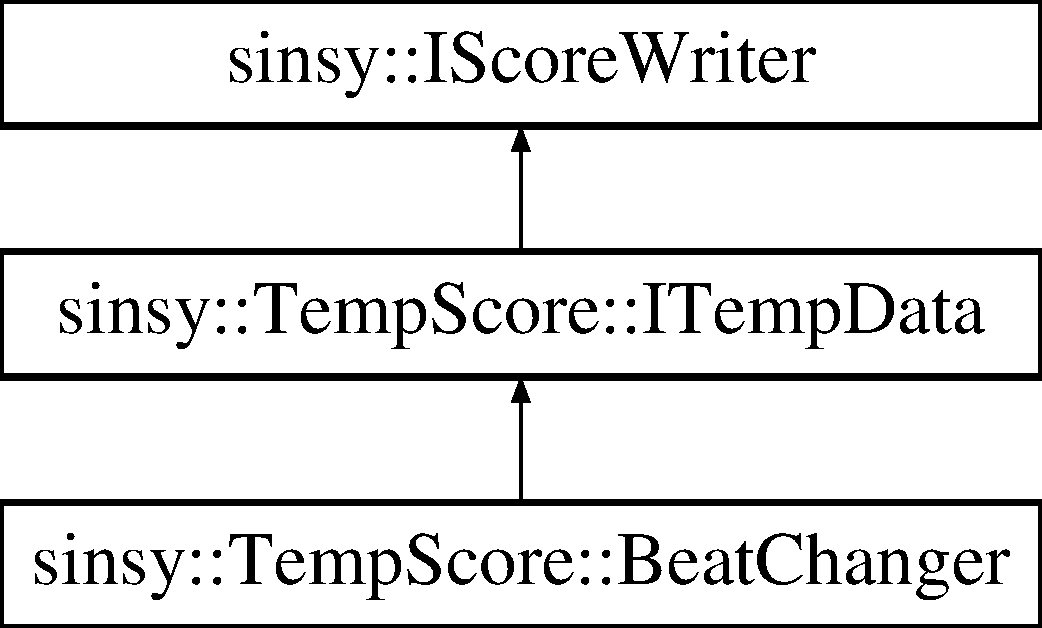
\includegraphics[height=3.000000cm]{classsinsy_1_1TempScore_1_1BeatChanger}
\end{center}
\end{figure}
\subsection*{\-Public \-Member \-Functions}
\begin{DoxyCompactItemize}
\item 
\hypertarget{classsinsy_1_1TempScore_1_1BeatChanger_ae4aae6a92ea81bd6f7be69738be89840}{\hyperlink{classsinsy_1_1TempScore_1_1BeatChanger_ae4aae6a92ea81bd6f7be69738be89840}{\-Beat\-Changer} (const \hyperlink{classsinsy_1_1Beat}{\-Beat} \&b)}\label{classsinsy_1_1TempScore_1_1BeatChanger_ae4aae6a92ea81bd6f7be69738be89840}

\begin{DoxyCompactList}\small\item\em constructor \end{DoxyCompactList}\item 
\hypertarget{classsinsy_1_1TempScore_1_1BeatChanger_aeeb6579ea768dc78960b1161501f0078}{virtual \hyperlink{classsinsy_1_1TempScore_1_1BeatChanger_aeeb6579ea768dc78960b1161501f0078}{$\sim$\-Beat\-Changer} ()}\label{classsinsy_1_1TempScore_1_1BeatChanger_aeeb6579ea768dc78960b1161501f0078}

\begin{DoxyCompactList}\small\item\em destructor \end{DoxyCompactList}\item 
\hypertarget{classsinsy_1_1TempScore_1_1BeatChanger_ae524ed795674a223d5dad411a063331d}{virtual void \hyperlink{classsinsy_1_1TempScore_1_1BeatChanger_ae524ed795674a223d5dad411a063331d}{write} (\hyperlink{classsinsy_1_1IScoreWritable}{\-I\-Score\-Writable} \&sm) const }\label{classsinsy_1_1TempScore_1_1BeatChanger_ae524ed795674a223d5dad411a063331d}

\begin{DoxyCompactList}\small\item\em write \end{DoxyCompactList}\end{DoxyCompactItemize}


\-The documentation for this class was generated from the following files\-:\begin{DoxyCompactItemize}
\item 
lib/temporary/\-Temp\-Score.\-h\item 
lib/temporary/\-Temp\-Score.\-cpp\end{DoxyCompactItemize}

\hypertarget{classsinsy_1_1ConfGroup}{\section{sinsy\-:\-:\-Conf\-Group \-Class \-Reference}
\label{classsinsy_1_1ConfGroup}\index{sinsy\-::\-Conf\-Group@{sinsy\-::\-Conf\-Group}}
}
\-Inheritance diagram for sinsy\-:\-:\-Conf\-Group\-:\begin{figure}[H]
\begin{center}
\leavevmode
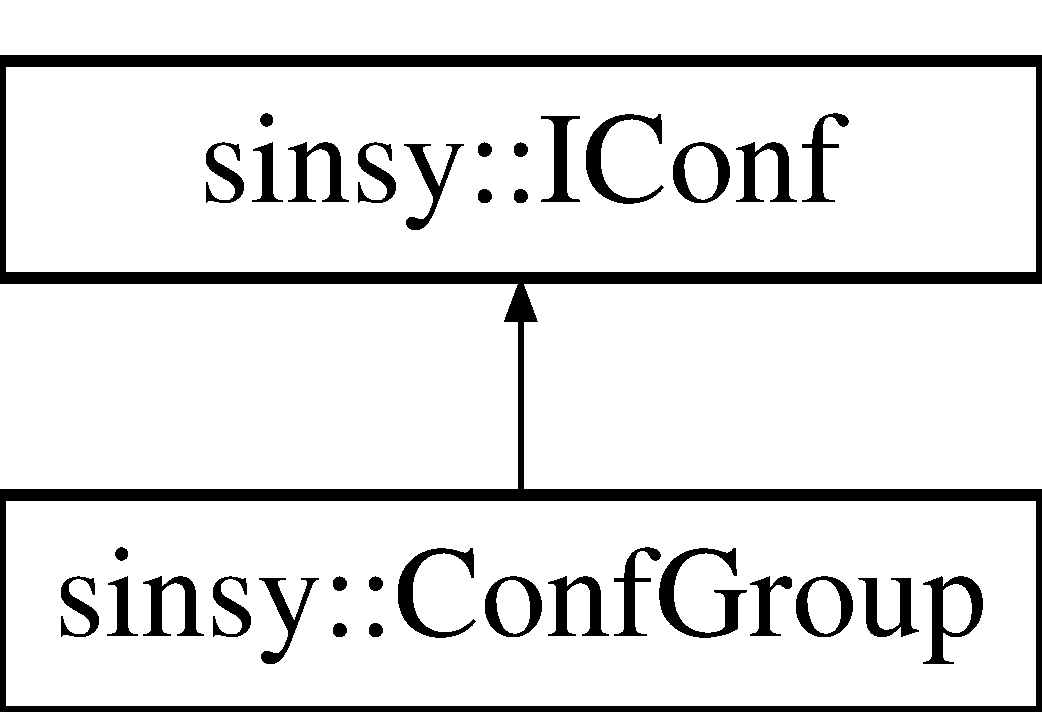
\includegraphics[height=2.000000cm]{classsinsy_1_1ConfGroup}
\end{center}
\end{figure}
\subsection*{\-Public \-Member \-Functions}
\begin{DoxyCompactItemize}
\item 
\hypertarget{classsinsy_1_1ConfGroup_a70489be741fc414c8471d64c090910b4}{\hyperlink{classsinsy_1_1ConfGroup_a70489be741fc414c8471d64c090910b4}{\-Conf\-Group} ()}\label{classsinsy_1_1ConfGroup_a70489be741fc414c8471d64c090910b4}

\begin{DoxyCompactList}\small\item\em constructor \end{DoxyCompactList}\item 
\hypertarget{classsinsy_1_1ConfGroup_aea251e5d8c5070e8dc367c42593c2066}{virtual \hyperlink{classsinsy_1_1ConfGroup_aea251e5d8c5070e8dc367c42593c2066}{$\sim$\-Conf\-Group} ()}\label{classsinsy_1_1ConfGroup_aea251e5d8c5070e8dc367c42593c2066}

\begin{DoxyCompactList}\small\item\em destructor \end{DoxyCompactList}\item 
void \hyperlink{classsinsy_1_1ConfGroup_afb98f9e41ce55a486e499e1a8bed08bd}{add} (const \hyperlink{classsinsy_1_1IConf}{\-I\-Conf} $\ast$conf)
\begin{DoxyCompactList}\small\item\em add conf \end{DoxyCompactList}\item 
\hypertarget{classsinsy_1_1ConfGroup_aa68bf11b21932c9a8d4f5e688c157c9c}{virtual bool \hyperlink{classsinsy_1_1ConfGroup_aa68bf11b21932c9a8d4f5e688c157c9c}{convert} (const std\-::string \&enc, \-Convertable\-List\-::iterator begin, \-Convertable\-List\-::iterator end) const }\label{classsinsy_1_1ConfGroup_aa68bf11b21932c9a8d4f5e688c157c9c}

\begin{DoxyCompactList}\small\item\em convert lyrics to phonemes \end{DoxyCompactList}\item 
\hypertarget{classsinsy_1_1ConfGroup_a72dc032a4cddb563c4d882488273a15b}{void \hyperlink{classsinsy_1_1ConfGroup_a72dc032a4cddb563c4d882488273a15b}{clear} ()}\label{classsinsy_1_1ConfGroup_a72dc032a4cddb563c4d882488273a15b}

\begin{DoxyCompactList}\small\item\em clear all confs \end{DoxyCompactList}\item 
\hypertarget{classsinsy_1_1ConfGroup_a9382fa2793abb32c0b1a7c649617cdde}{virtual std\-::string \hyperlink{classsinsy_1_1ConfGroup_a9382fa2793abb32c0b1a7c649617cdde}{get\-Sil\-Str} () const }\label{classsinsy_1_1ConfGroup_a9382fa2793abb32c0b1a7c649617cdde}

\begin{DoxyCompactList}\small\item\em get sil string \end{DoxyCompactList}\end{DoxyCompactItemize}


\subsection{\-Member \-Function \-Documentation}
\hypertarget{classsinsy_1_1ConfGroup_afb98f9e41ce55a486e499e1a8bed08bd}{\index{sinsy\-::\-Conf\-Group@{sinsy\-::\-Conf\-Group}!add@{add}}
\index{add@{add}!sinsy::ConfGroup@{sinsy\-::\-Conf\-Group}}
\subsubsection[{add}]{\setlength{\rightskip}{0pt plus 5cm}void {\bf \-Conf\-Group\-::add} (
\begin{DoxyParamCaption}
\item[{const {\bf \-I\-Conf} $\ast$}]{conf}
\end{DoxyParamCaption}
)}}\label{classsinsy_1_1ConfGroup_afb98f9e41ce55a486e499e1a8bed08bd}


add conf 

add config 

\-The documentation for this class was generated from the following files\-:\begin{DoxyCompactItemize}
\item 
lib/converter/\-Conf\-Group.\-h\item 
lib/converter/\-Conf\-Group.\-cpp\end{DoxyCompactItemize}

\hypertarget{classsinsy_1_1Configurations}{\section{sinsy\-:\-:\-Configurations \-Class \-Reference}
\label{classsinsy_1_1Configurations}\index{sinsy\-::\-Configurations@{sinsy\-::\-Configurations}}
}
\subsection*{\-Public \-Member \-Functions}
\begin{DoxyCompactItemize}
\item 
\hypertarget{classsinsy_1_1Configurations_ae8bdd24e3f76262c0aa3518ceabc4731}{\hyperlink{classsinsy_1_1Configurations_ae8bdd24e3f76262c0aa3518ceabc4731}{\-Configurations} ()}\label{classsinsy_1_1Configurations_ae8bdd24e3f76262c0aa3518ceabc4731}

\begin{DoxyCompactList}\small\item\em constructor \end{DoxyCompactList}\item 
\hypertarget{classsinsy_1_1Configurations_ab936418c05ff482a0da4963148cbb264}{virtual \hyperlink{classsinsy_1_1Configurations_ab936418c05ff482a0da4963148cbb264}{$\sim$\-Configurations} ()}\label{classsinsy_1_1Configurations_ab936418c05ff482a0da4963148cbb264}

\begin{DoxyCompactList}\small\item\em destructor \end{DoxyCompactList}\item 
\hypertarget{classsinsy_1_1Configurations_a15db5511620326d0daadf2d8d584f070}{void \hyperlink{classsinsy_1_1Configurations_a15db5511620326d0daadf2d8d584f070}{clear} ()}\label{classsinsy_1_1Configurations_a15db5511620326d0daadf2d8d584f070}

\begin{DoxyCompactList}\small\item\em clear \end{DoxyCompactList}\item 
\hypertarget{classsinsy_1_1Configurations_ad58be2d0caca2befe358ce443717c11b}{bool \hyperlink{classsinsy_1_1Configurations_ad58be2d0caca2befe358ce443717c11b}{read} (const std\-::string \&fpath)}\label{classsinsy_1_1Configurations_ad58be2d0caca2befe358ce443717c11b}

\begin{DoxyCompactList}\small\item\em read configurations from file \end{DoxyCompactList}\item 
{\footnotesize template$<$class T $>$ }\\\-T \hyperlink{classsinsy_1_1Configurations_a37140fb4d61c28384fdabb51a84b21b2}{get} (const std\-::string \&, const \-T \&) const 
\begin{DoxyCompactList}\small\item\em get \end{DoxyCompactList}\item 
std\-::string \hyperlink{classsinsy_1_1Configurations_a022a2fa94236656f078dd2b680d3b4e3}{get} (const std\-::string \&) const 
\begin{DoxyCompactList}\small\item\em get \end{DoxyCompactList}\item 
{\footnotesize template$<$$>$ }\\bool \hyperlink{classsinsy_1_1Configurations_a96907af75d2c3dcef8c200f2d4f651f9}{get} (const std\-::string \&key, const bool \&def) const 
\item 
{\footnotesize template$<$$>$ }\\bool \hyperlink{classsinsy_1_1Configurations_a96907af75d2c3dcef8c200f2d4f651f9}{get} (const std\-::string \&key, const bool \&def) const 
\end{DoxyCompactItemize}


\subsection{\-Member \-Function \-Documentation}
\hypertarget{classsinsy_1_1Configurations_a37140fb4d61c28384fdabb51a84b21b2}{\index{sinsy\-::\-Configurations@{sinsy\-::\-Configurations}!get@{get}}
\index{get@{get}!sinsy::Configurations@{sinsy\-::\-Configurations}}
\subsubsection[{get}]{\setlength{\rightskip}{0pt plus 5cm}template$<$class T $>$ \-T {\bf sinsy\-::\-Configurations\-::get} (
\begin{DoxyParamCaption}
\item[{const std\-::string \&}]{key, }
\item[{const \-T \&}]{def}
\end{DoxyParamCaption}
) const}}\label{classsinsy_1_1Configurations_a37140fb4d61c28384fdabb51a84b21b2}


get 

get


\begin{DoxyParams}{\-Parameters}
{\em key} & \\
\hline
{\em def} & default value \\
\hline
\end{DoxyParams}
\begin{DoxyReturn}{\-Returns}

\end{DoxyReturn}
\hypertarget{classsinsy_1_1Configurations_a022a2fa94236656f078dd2b680d3b4e3}{\index{sinsy\-::\-Configurations@{sinsy\-::\-Configurations}!get@{get}}
\index{get@{get}!sinsy::Configurations@{sinsy\-::\-Configurations}}
\subsubsection[{get}]{\setlength{\rightskip}{0pt plus 5cm}std\-::string {\bf \-Configurations\-::get} (
\begin{DoxyParamCaption}
\item[{const std\-::string \&}]{key}
\end{DoxyParamCaption}
) const}}\label{classsinsy_1_1Configurations_a022a2fa94236656f078dd2b680d3b4e3}


get 

for std\-::string (not need default) \hypertarget{classsinsy_1_1Configurations_a96907af75d2c3dcef8c200f2d4f651f9}{\index{sinsy\-::\-Configurations@{sinsy\-::\-Configurations}!get@{get}}
\index{get@{get}!sinsy::Configurations@{sinsy\-::\-Configurations}}
\subsubsection[{get}]{\setlength{\rightskip}{0pt plus 5cm}template$<$$>$ bool {\bf sinsy\-::\-Configurations\-::get} (
\begin{DoxyParamCaption}
\item[{const std\-::string \&}]{key, }
\item[{const bool \&}]{def}
\end{DoxyParamCaption}
) const}}\label{classsinsy_1_1Configurations_a96907af75d2c3dcef8c200f2d4f651f9}
get (bool) \hypertarget{classsinsy_1_1Configurations_a96907af75d2c3dcef8c200f2d4f651f9}{\index{sinsy\-::\-Configurations@{sinsy\-::\-Configurations}!get@{get}}
\index{get@{get}!sinsy::Configurations@{sinsy\-::\-Configurations}}
\subsubsection[{get}]{\setlength{\rightskip}{0pt plus 5cm}template$<$$>$ bool {\bf sinsy\-::\-Configurations\-::get} (
\begin{DoxyParamCaption}
\item[{const std\-::string \&}]{key, }
\item[{const bool \&}]{def}
\end{DoxyParamCaption}
) const}}\label{classsinsy_1_1Configurations_a96907af75d2c3dcef8c200f2d4f651f9}
for bool 

\-The documentation for this class was generated from the following files\-:\begin{DoxyCompactItemize}
\item 
lib/util/\-Configurations.\-h\item 
lib/util/\-Configurations.\-cpp\end{DoxyCompactItemize}

\hypertarget{classsinsy_1_1ConfManager}{\section{sinsy\-:\-:\-Conf\-Manager \-Class \-Reference}
\label{classsinsy_1_1ConfManager}\index{sinsy\-::\-Conf\-Manager@{sinsy\-::\-Conf\-Manager}}
}
\subsection*{\-Public \-Member \-Functions}
\begin{DoxyCompactItemize}
\item 
\hypertarget{classsinsy_1_1ConfManager_a8aeadd9e65e39448f396409a4ce942c7}{\hyperlink{classsinsy_1_1ConfManager_a8aeadd9e65e39448f396409a4ce942c7}{\-Conf\-Manager} ()}\label{classsinsy_1_1ConfManager_a8aeadd9e65e39448f396409a4ce942c7}

\begin{DoxyCompactList}\small\item\em constructor \end{DoxyCompactList}\item 
\hypertarget{classsinsy_1_1ConfManager_a6b9b153b626970bd563d290cdf5181c7}{virtual \hyperlink{classsinsy_1_1ConfManager_a6b9b153b626970bd563d290cdf5181c7}{$\sim$\-Conf\-Manager} ()}\label{classsinsy_1_1ConfManager_a6b9b153b626970bd563d290cdf5181c7}

\begin{DoxyCompactList}\small\item\em destructor \end{DoxyCompactList}\item 
bool \hyperlink{classsinsy_1_1ConfManager_a22f9ffc02ed91affdd3aef73b0f6e9ff}{set\-Languages} (const std\-::string \&languages, const std\-::string \&dir\-Path)
\begin{DoxyCompactList}\small\item\em set confs to converter \end{DoxyCompactList}\item 
\hypertarget{classsinsy_1_1ConfManager_a8554d398c696992d776d6ba28447e7f5}{void \hyperlink{classsinsy_1_1ConfManager_a8554d398c696992d776d6ba28447e7f5}{set\-Default\-Confs} (\hyperlink{classsinsy_1_1ConfGroup}{\-Conf\-Group} \&confs) const }\label{classsinsy_1_1ConfManager_a8554d398c696992d776d6ba28447e7f5}

\begin{DoxyCompactList}\small\item\em set default confs \end{DoxyCompactList}\end{DoxyCompactItemize}


\subsection{\-Member \-Function \-Documentation}
\hypertarget{classsinsy_1_1ConfManager_a22f9ffc02ed91affdd3aef73b0f6e9ff}{\index{sinsy\-::\-Conf\-Manager@{sinsy\-::\-Conf\-Manager}!set\-Languages@{set\-Languages}}
\index{set\-Languages@{set\-Languages}!sinsy::ConfManager@{sinsy\-::\-Conf\-Manager}}
\subsubsection[{set\-Languages}]{\setlength{\rightskip}{0pt plus 5cm}bool {\bf \-Conf\-Manager\-::set\-Languages} (
\begin{DoxyParamCaption}
\item[{const std\-::string \&}]{languages, }
\item[{const std\-::string \&}]{dir\-Path}
\end{DoxyParamCaption}
)}}\label{classsinsy_1_1ConfManager_a22f9ffc02ed91affdd3aef73b0f6e9ff}


set confs to converter 

set languages (\-Currently, you can set only \-Japanese (j)) 

\-The documentation for this class was generated from the following files\-:\begin{DoxyCompactItemize}
\item 
lib/converter/\-Conf\-Manager.\-h\item 
lib/converter/\-Conf\-Manager.\-cpp\end{DoxyCompactItemize}

\hypertarget{classsinsy_1_1Converter}{\section{sinsy\-:\-:\-Converter \-Class \-Reference}
\label{classsinsy_1_1Converter}\index{sinsy\-::\-Converter@{sinsy\-::\-Converter}}
}
\subsection*{\-Public \-Member \-Functions}
\begin{DoxyCompactItemize}
\item 
\hypertarget{classsinsy_1_1Converter_a1de81f3e06093411e5d27ce882bc010f}{\hyperlink{classsinsy_1_1Converter_a1de81f3e06093411e5d27ce882bc010f}{\-Converter} ()}\label{classsinsy_1_1Converter_a1de81f3e06093411e5d27ce882bc010f}

\begin{DoxyCompactList}\small\item\em constructor \end{DoxyCompactList}\item 
\hypertarget{classsinsy_1_1Converter_a9ecd05695a52c03158b81e544e13b996}{virtual \hyperlink{classsinsy_1_1Converter_a9ecd05695a52c03158b81e544e13b996}{$\sim$\-Converter} ()}\label{classsinsy_1_1Converter_a9ecd05695a52c03158b81e544e13b996}

\begin{DoxyCompactList}\small\item\em destructor \end{DoxyCompactList}\item 
\hypertarget{classsinsy_1_1Converter_a7b2caf7931deed5f5ff1be9e04225743}{void \hyperlink{classsinsy_1_1Converter_a7b2caf7931deed5f5ff1be9e04225743}{clear} ()}\label{classsinsy_1_1Converter_a7b2caf7931deed5f5ff1be9e04225743}

\begin{DoxyCompactList}\small\item\em clear \end{DoxyCompactList}\item 
\hypertarget{classsinsy_1_1Converter_a5ab31f8f1e79953f60d2c48485ed4ee5}{bool \hyperlink{classsinsy_1_1Converter_a5ab31f8f1e79953f60d2c48485ed4ee5}{set\-Languages} (const std\-::string \&languages, const std\-::string \&dir\-Path)}\label{classsinsy_1_1Converter_a5ab31f8f1e79953f60d2c48485ed4ee5}

\begin{DoxyCompactList}\small\item\em set confs to converter \end{DoxyCompactList}\item 
std\-::string \hyperlink{classsinsy_1_1Converter_a4ca7b9b2172c31a3ed73ab09d5180b91}{get\-Sil\-Str} () const 
\begin{DoxyCompactList}\small\item\em get sil str \end{DoxyCompactList}\item 
\hypertarget{classsinsy_1_1Converter_a313eaec8b1ac0bd30de73e2d0f6ab268}{virtual bool \hyperlink{classsinsy_1_1Converter_a313eaec8b1ac0bd30de73e2d0f6ab268}{convert} (const std\-::string \&enc, \-I\-Conf\-::\-Convertable\-List\-::iterator begin, \-I\-Conf\-::\-Convertable\-List\-::iterator end) const }\label{classsinsy_1_1Converter_a313eaec8b1ac0bd30de73e2d0f6ab268}

\begin{DoxyCompactList}\small\item\em convert \end{DoxyCompactList}\end{DoxyCompactItemize}


\subsection{\-Member \-Function \-Documentation}
\hypertarget{classsinsy_1_1Converter_a4ca7b9b2172c31a3ed73ab09d5180b91}{\index{sinsy\-::\-Converter@{sinsy\-::\-Converter}!get\-Sil\-Str@{get\-Sil\-Str}}
\index{get\-Sil\-Str@{get\-Sil\-Str}!sinsy::Converter@{sinsy\-::\-Converter}}
\subsubsection[{get\-Sil\-Str}]{\setlength{\rightskip}{0pt plus 5cm}std\-::string {\bf \-Converter\-::get\-Sil\-Str} (
\begin{DoxyParamCaption}
{}
\end{DoxyParamCaption}
) const}}\label{classsinsy_1_1Converter_a4ca7b9b2172c31a3ed73ab09d5180b91}


get sil str 

get sil string 

\-The documentation for this class was generated from the following files\-:\begin{DoxyCompactItemize}
\item 
lib/converter/\-Converter.\-h\item 
lib/converter/\-Converter.\-cpp\end{DoxyCompactItemize}

\hypertarget{classsinsy_1_1TempScore_1_1CrescendoStarter}{\section{sinsy\-:\-:\-Temp\-Score\-:\-:\-Crescendo\-Starter \-Class \-Reference}
\label{classsinsy_1_1TempScore_1_1CrescendoStarter}\index{sinsy\-::\-Temp\-Score\-::\-Crescendo\-Starter@{sinsy\-::\-Temp\-Score\-::\-Crescendo\-Starter}}
}
\-Inheritance diagram for sinsy\-:\-:\-Temp\-Score\-:\-:\-Crescendo\-Starter\-:\begin{figure}[H]
\begin{center}
\leavevmode
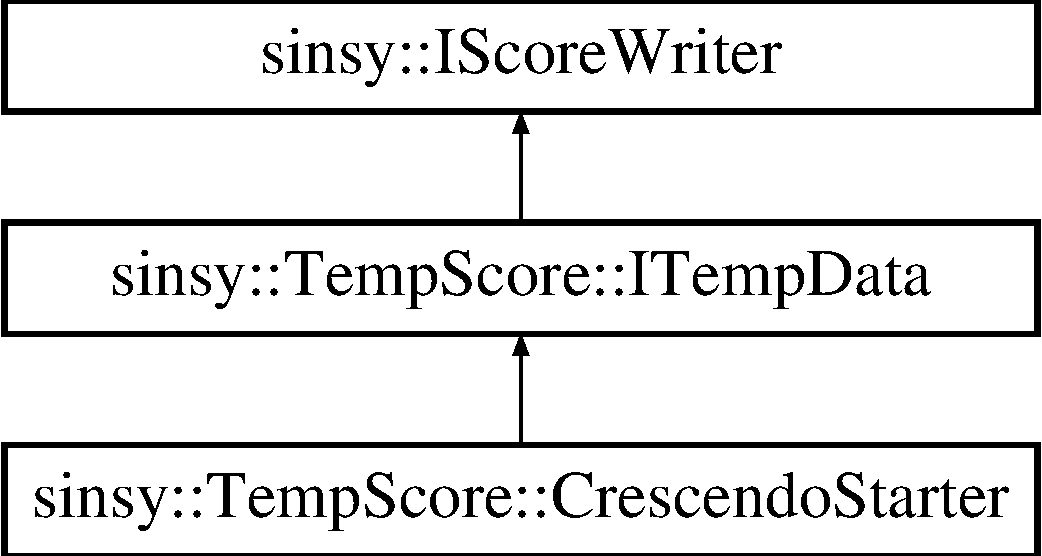
\includegraphics[height=3.000000cm]{classsinsy_1_1TempScore_1_1CrescendoStarter}
\end{center}
\end{figure}
\subsection*{\-Public \-Member \-Functions}
\begin{DoxyCompactItemize}
\item 
\hypertarget{classsinsy_1_1TempScore_1_1CrescendoStarter_a4381cb2cc61856ee2e992eb1eecb4b0b}{\hyperlink{classsinsy_1_1TempScore_1_1CrescendoStarter_a4381cb2cc61856ee2e992eb1eecb4b0b}{\-Crescendo\-Starter} ()}\label{classsinsy_1_1TempScore_1_1CrescendoStarter_a4381cb2cc61856ee2e992eb1eecb4b0b}

\begin{DoxyCompactList}\small\item\em constructor \end{DoxyCompactList}\item 
\hypertarget{classsinsy_1_1TempScore_1_1CrescendoStarter_a04f9cc7926c84987755085f449adb3aa}{virtual \hyperlink{classsinsy_1_1TempScore_1_1CrescendoStarter_a04f9cc7926c84987755085f449adb3aa}{$\sim$\-Crescendo\-Starter} ()}\label{classsinsy_1_1TempScore_1_1CrescendoStarter_a04f9cc7926c84987755085f449adb3aa}

\begin{DoxyCompactList}\small\item\em destructor \end{DoxyCompactList}\item 
\hypertarget{classsinsy_1_1TempScore_1_1CrescendoStarter_a0b75a155b850ea55d3a0fac5f2cbed0a}{virtual void \hyperlink{classsinsy_1_1TempScore_1_1CrescendoStarter_a0b75a155b850ea55d3a0fac5f2cbed0a}{write} (\hyperlink{classsinsy_1_1IScoreWritable}{\-I\-Score\-Writable} \&sm) const }\label{classsinsy_1_1TempScore_1_1CrescendoStarter_a0b75a155b850ea55d3a0fac5f2cbed0a}

\begin{DoxyCompactList}\small\item\em write \end{DoxyCompactList}\end{DoxyCompactItemize}


\-The documentation for this class was generated from the following files\-:\begin{DoxyCompactItemize}
\item 
lib/temporary/\-Temp\-Score.\-h\item 
lib/temporary/\-Temp\-Score.\-cpp\end{DoxyCompactItemize}

\hypertarget{classsinsy_1_1TempScore_1_1CrescendoStopper}{\section{sinsy\-:\-:\-Temp\-Score\-:\-:\-Crescendo\-Stopper \-Class \-Reference}
\label{classsinsy_1_1TempScore_1_1CrescendoStopper}\index{sinsy\-::\-Temp\-Score\-::\-Crescendo\-Stopper@{sinsy\-::\-Temp\-Score\-::\-Crescendo\-Stopper}}
}
\-Inheritance diagram for sinsy\-:\-:\-Temp\-Score\-:\-:\-Crescendo\-Stopper\-:\begin{figure}[H]
\begin{center}
\leavevmode
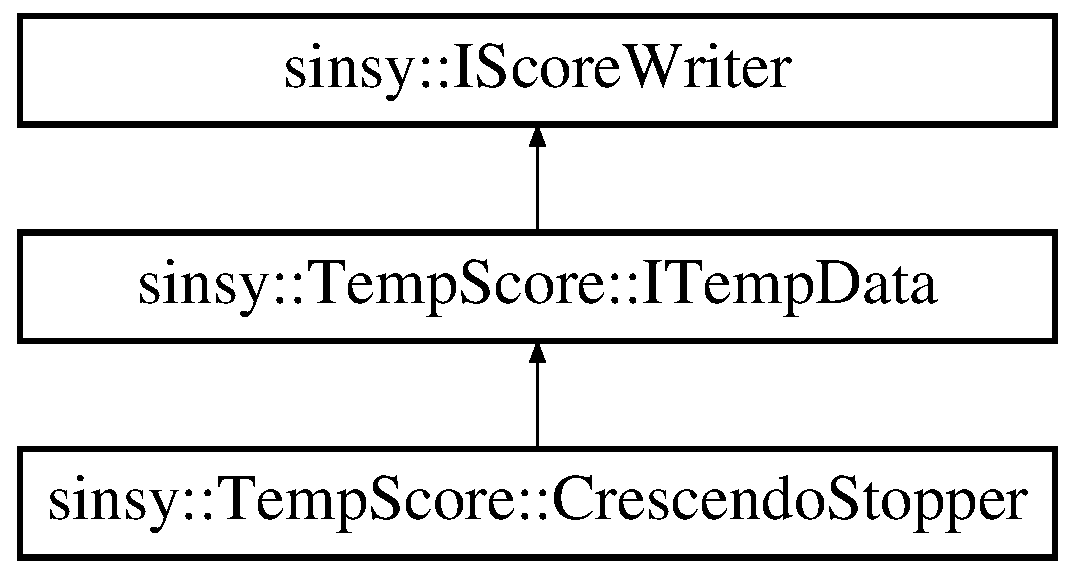
\includegraphics[height=3.000000cm]{classsinsy_1_1TempScore_1_1CrescendoStopper}
\end{center}
\end{figure}
\subsection*{\-Public \-Member \-Functions}
\begin{DoxyCompactItemize}
\item 
\hypertarget{classsinsy_1_1TempScore_1_1CrescendoStopper_a6fa1c3f68c4a760405ae72b131051fbd}{\hyperlink{classsinsy_1_1TempScore_1_1CrescendoStopper_a6fa1c3f68c4a760405ae72b131051fbd}{\-Crescendo\-Stopper} ()}\label{classsinsy_1_1TempScore_1_1CrescendoStopper_a6fa1c3f68c4a760405ae72b131051fbd}

\begin{DoxyCompactList}\small\item\em constructor \end{DoxyCompactList}\item 
\hypertarget{classsinsy_1_1TempScore_1_1CrescendoStopper_af1f1f4adb187c28592d56fc5d1ecbc42}{virtual \hyperlink{classsinsy_1_1TempScore_1_1CrescendoStopper_af1f1f4adb187c28592d56fc5d1ecbc42}{$\sim$\-Crescendo\-Stopper} ()}\label{classsinsy_1_1TempScore_1_1CrescendoStopper_af1f1f4adb187c28592d56fc5d1ecbc42}

\begin{DoxyCompactList}\small\item\em destructor \end{DoxyCompactList}\item 
\hypertarget{classsinsy_1_1TempScore_1_1CrescendoStopper_a1f99db8f1dc132386435e1b2c242341a}{virtual void \hyperlink{classsinsy_1_1TempScore_1_1CrescendoStopper_a1f99db8f1dc132386435e1b2c242341a}{write} (\hyperlink{classsinsy_1_1IScoreWritable}{\-I\-Score\-Writable} \&sm) const }\label{classsinsy_1_1TempScore_1_1CrescendoStopper_a1f99db8f1dc132386435e1b2c242341a}

\begin{DoxyCompactList}\small\item\em write \end{DoxyCompactList}\end{DoxyCompactItemize}


\-The documentation for this class was generated from the following files\-:\begin{DoxyCompactItemize}
\item 
lib/temporary/\-Temp\-Score.\-h\item 
lib/temporary/\-Temp\-Score.\-cpp\end{DoxyCompactItemize}

\hypertarget{classsinsy_1_1Deleter}{\section{sinsy\-:\-:\-Deleter$<$ \-T $>$ \-Class \-Template \-Reference}
\label{classsinsy_1_1Deleter}\index{sinsy\-::\-Deleter$<$ T $>$@{sinsy\-::\-Deleter$<$ T $>$}}
}


{\ttfamily \#include $<$\-Deleter.\-h$>$}

\subsection*{\-Public \-Member \-Functions}
\begin{DoxyCompactItemize}
\item 
\hypertarget{classsinsy_1_1Deleter_abac45b967afd9f06171d326db269b60e}{\hyperlink{classsinsy_1_1Deleter_abac45b967afd9f06171d326db269b60e}{\-Deleter} ()}\label{classsinsy_1_1Deleter_abac45b967afd9f06171d326db269b60e}

\begin{DoxyCompactList}\small\item\em constructor \end{DoxyCompactList}\item 
\hypertarget{classsinsy_1_1Deleter_a88dd86effe16835507c2976ac8f7395e}{virtual \hyperlink{classsinsy_1_1Deleter_a88dd86effe16835507c2976ac8f7395e}{$\sim$\-Deleter} ()}\label{classsinsy_1_1Deleter_a88dd86effe16835507c2976ac8f7395e}

\begin{DoxyCompactList}\small\item\em destructor \end{DoxyCompactList}\item 
\hypertarget{classsinsy_1_1Deleter_aacfabd0bf43f568b6fe6269e87cf30be}{void \hyperlink{classsinsy_1_1Deleter_aacfabd0bf43f568b6fe6269e87cf30be}{operator()} (\-T $\ast$pointer)}\label{classsinsy_1_1Deleter_aacfabd0bf43f568b6fe6269e87cf30be}

\begin{DoxyCompactList}\small\item\em ... \end{DoxyCompactList}\end{DoxyCompactItemize}


\subsection{\-Detailed \-Description}
\subsubsection*{template$<$class T$>$class sinsy\-::\-Deleter$<$ T $>$}

deleter 

\-The documentation for this class was generated from the following file\-:\begin{DoxyCompactItemize}
\item 
lib/util/\-Deleter.\-h\end{DoxyCompactItemize}

\hypertarget{classsinsy_1_1TempScore_1_1DiminuendoStarter}{\section{sinsy\-:\-:\-Temp\-Score\-:\-:\-Diminuendo\-Starter \-Class \-Reference}
\label{classsinsy_1_1TempScore_1_1DiminuendoStarter}\index{sinsy\-::\-Temp\-Score\-::\-Diminuendo\-Starter@{sinsy\-::\-Temp\-Score\-::\-Diminuendo\-Starter}}
}
\-Inheritance diagram for sinsy\-:\-:\-Temp\-Score\-:\-:\-Diminuendo\-Starter\-:\begin{figure}[H]
\begin{center}
\leavevmode
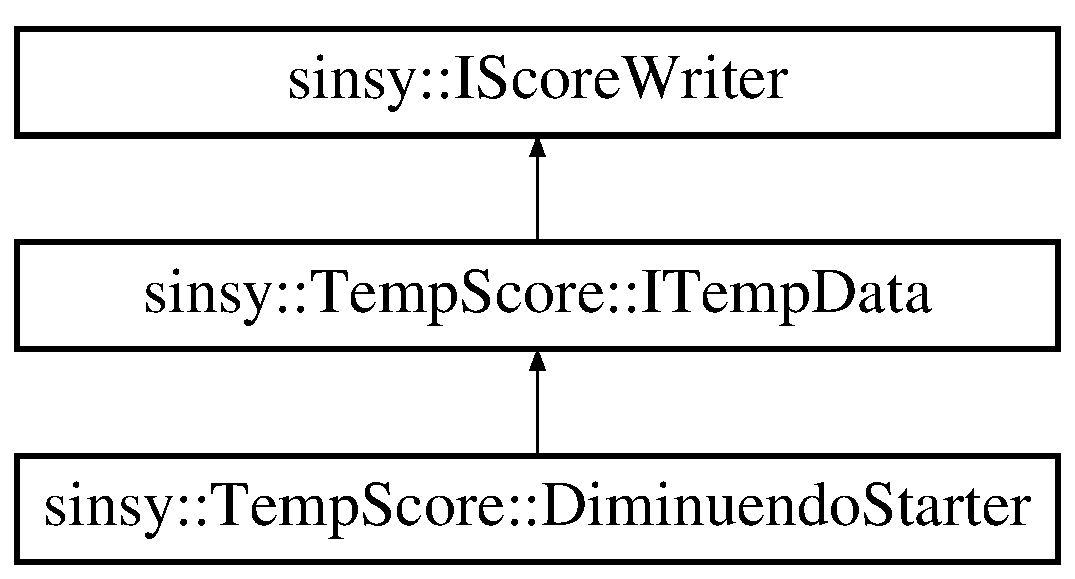
\includegraphics[height=3.000000cm]{classsinsy_1_1TempScore_1_1DiminuendoStarter}
\end{center}
\end{figure}
\subsection*{\-Public \-Member \-Functions}
\begin{DoxyCompactItemize}
\item 
\hypertarget{classsinsy_1_1TempScore_1_1DiminuendoStarter_a2a8cccbd3cd8499deedd31c14e17b207}{\hyperlink{classsinsy_1_1TempScore_1_1DiminuendoStarter_a2a8cccbd3cd8499deedd31c14e17b207}{\-Diminuendo\-Starter} ()}\label{classsinsy_1_1TempScore_1_1DiminuendoStarter_a2a8cccbd3cd8499deedd31c14e17b207}

\begin{DoxyCompactList}\small\item\em constructor \end{DoxyCompactList}\item 
\hypertarget{classsinsy_1_1TempScore_1_1DiminuendoStarter_ad6ad437359e571a6f23acb5544d91e70}{virtual \hyperlink{classsinsy_1_1TempScore_1_1DiminuendoStarter_ad6ad437359e571a6f23acb5544d91e70}{$\sim$\-Diminuendo\-Starter} ()}\label{classsinsy_1_1TempScore_1_1DiminuendoStarter_ad6ad437359e571a6f23acb5544d91e70}

\begin{DoxyCompactList}\small\item\em destructor \end{DoxyCompactList}\item 
\hypertarget{classsinsy_1_1TempScore_1_1DiminuendoStarter_ad2f63339280fe4defc467118606a97f8}{virtual void \hyperlink{classsinsy_1_1TempScore_1_1DiminuendoStarter_ad2f63339280fe4defc467118606a97f8}{write} (\hyperlink{classsinsy_1_1IScoreWritable}{\-I\-Score\-Writable} \&sm) const }\label{classsinsy_1_1TempScore_1_1DiminuendoStarter_ad2f63339280fe4defc467118606a97f8}

\begin{DoxyCompactList}\small\item\em write \end{DoxyCompactList}\end{DoxyCompactItemize}


\-The documentation for this class was generated from the following files\-:\begin{DoxyCompactItemize}
\item 
lib/temporary/\-Temp\-Score.\-h\item 
lib/temporary/\-Temp\-Score.\-cpp\end{DoxyCompactItemize}

\hypertarget{classsinsy_1_1TempScore_1_1DiminuendoStopper}{\section{sinsy\-:\-:\-Temp\-Score\-:\-:\-Diminuendo\-Stopper \-Class \-Reference}
\label{classsinsy_1_1TempScore_1_1DiminuendoStopper}\index{sinsy\-::\-Temp\-Score\-::\-Diminuendo\-Stopper@{sinsy\-::\-Temp\-Score\-::\-Diminuendo\-Stopper}}
}
\-Inheritance diagram for sinsy\-:\-:\-Temp\-Score\-:\-:\-Diminuendo\-Stopper\-:\begin{figure}[H]
\begin{center}
\leavevmode
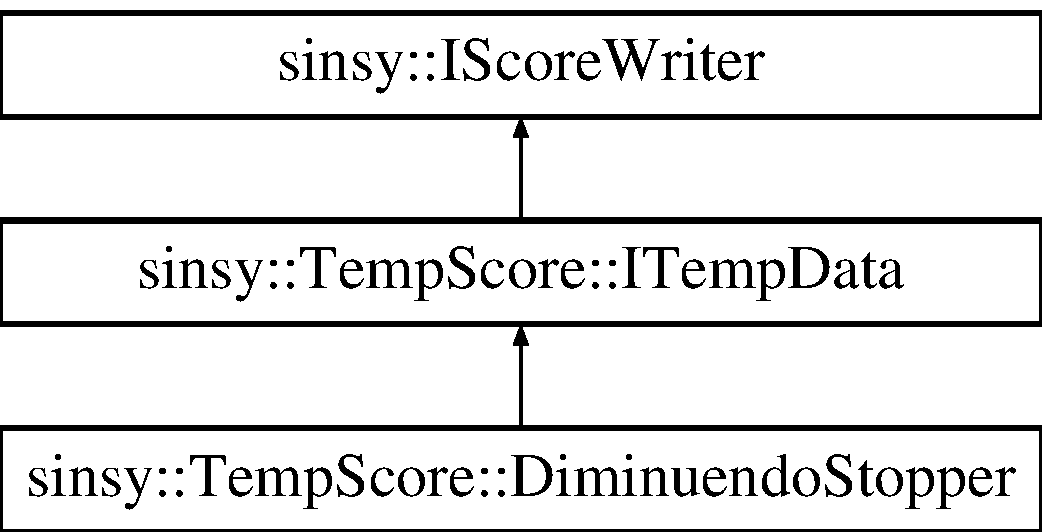
\includegraphics[height=3.000000cm]{classsinsy_1_1TempScore_1_1DiminuendoStopper}
\end{center}
\end{figure}
\subsection*{\-Public \-Member \-Functions}
\begin{DoxyCompactItemize}
\item 
\hypertarget{classsinsy_1_1TempScore_1_1DiminuendoStopper_ad018ff485c9826001270c12b9a7b3d31}{\hyperlink{classsinsy_1_1TempScore_1_1DiminuendoStopper_ad018ff485c9826001270c12b9a7b3d31}{\-Diminuendo\-Stopper} ()}\label{classsinsy_1_1TempScore_1_1DiminuendoStopper_ad018ff485c9826001270c12b9a7b3d31}

\begin{DoxyCompactList}\small\item\em constructor \end{DoxyCompactList}\item 
\hypertarget{classsinsy_1_1TempScore_1_1DiminuendoStopper_a783373c3255e7b819c9e8a4b52363c1e}{virtual \hyperlink{classsinsy_1_1TempScore_1_1DiminuendoStopper_a783373c3255e7b819c9e8a4b52363c1e}{$\sim$\-Diminuendo\-Stopper} ()}\label{classsinsy_1_1TempScore_1_1DiminuendoStopper_a783373c3255e7b819c9e8a4b52363c1e}

\begin{DoxyCompactList}\small\item\em destructor \end{DoxyCompactList}\item 
\hypertarget{classsinsy_1_1TempScore_1_1DiminuendoStopper_a89abf91b595eb10415fed8cacb1f10eb}{virtual void \hyperlink{classsinsy_1_1TempScore_1_1DiminuendoStopper_a89abf91b595eb10415fed8cacb1f10eb}{write} (\hyperlink{classsinsy_1_1IScoreWritable}{\-I\-Score\-Writable} \&sm) const }\label{classsinsy_1_1TempScore_1_1DiminuendoStopper_a89abf91b595eb10415fed8cacb1f10eb}

\begin{DoxyCompactList}\small\item\em write \end{DoxyCompactList}\end{DoxyCompactItemize}


\-The documentation for this class was generated from the following files\-:\begin{DoxyCompactItemize}
\item 
lib/temporary/\-Temp\-Score.\-h\item 
lib/temporary/\-Temp\-Score.\-cpp\end{DoxyCompactItemize}

\hypertarget{classsinsy_1_1Dynamics}{\section{sinsy\-:\-:\-Dynamics \-Class \-Reference}
\label{classsinsy_1_1Dynamics}\index{sinsy\-::\-Dynamics@{sinsy\-::\-Dynamics}}
}
\subsection*{\-Public \-Member \-Functions}
\begin{DoxyCompactItemize}
\item 
\hypertarget{classsinsy_1_1Dynamics_af3e1536fbe0ac872e65d1b0d5b8867a8}{\hyperlink{classsinsy_1_1Dynamics_af3e1536fbe0ac872e65d1b0d5b8867a8}{\-Dynamics} ()}\label{classsinsy_1_1Dynamics_af3e1536fbe0ac872e65d1b0d5b8867a8}

\begin{DoxyCompactList}\small\item\em constructor \end{DoxyCompactList}\item 
\hypertarget{classsinsy_1_1Dynamics_a70063e6a07a586e38a57a56fae382661}{\hyperlink{classsinsy_1_1Dynamics_a70063e6a07a586e38a57a56fae382661}{\-Dynamics} (const std\-::string \&str)}\label{classsinsy_1_1Dynamics_a70063e6a07a586e38a57a56fae382661}

\begin{DoxyCompactList}\small\item\em constructor \end{DoxyCompactList}\item 
\hypertarget{classsinsy_1_1Dynamics_ae5cd878f576a562b3c6096d9a0ebf4f6}{\hyperlink{classsinsy_1_1Dynamics_ae5cd878f576a562b3c6096d9a0ebf4f6}{\-Dynamics} (const \hyperlink{classsinsy_1_1Dynamics}{\-Dynamics} \&obj)}\label{classsinsy_1_1Dynamics_ae5cd878f576a562b3c6096d9a0ebf4f6}

\begin{DoxyCompactList}\small\item\em copy constructor \end{DoxyCompactList}\item 
\hypertarget{classsinsy_1_1Dynamics_ad06eca3d16f785f765235effe3047bcf}{virtual \hyperlink{classsinsy_1_1Dynamics_ad06eca3d16f785f765235effe3047bcf}{$\sim$\-Dynamics} ()}\label{classsinsy_1_1Dynamics_ad06eca3d16f785f765235effe3047bcf}

\begin{DoxyCompactList}\small\item\em destructor \end{DoxyCompactList}\item 
\hypertarget{classsinsy_1_1Dynamics_ae1a0ae4764c32f96670572d592292554}{\hyperlink{classsinsy_1_1Dynamics}{\-Dynamics} \& \hyperlink{classsinsy_1_1Dynamics_ae1a0ae4764c32f96670572d592292554}{operator=} (const \hyperlink{classsinsy_1_1Dynamics}{\-Dynamics} \&obj)}\label{classsinsy_1_1Dynamics_ae1a0ae4764c32f96670572d592292554}

\begin{DoxyCompactList}\small\item\em assignment operator \end{DoxyCompactList}\item 
\hypertarget{classsinsy_1_1Dynamics_a8fd4e333e8093696a6d37fca65135cb0}{bool \hyperlink{classsinsy_1_1Dynamics_a8fd4e333e8093696a6d37fca65135cb0}{operator==} (const \hyperlink{classsinsy_1_1Dynamics}{\-Dynamics} \&obj) const }\label{classsinsy_1_1Dynamics_a8fd4e333e8093696a6d37fca65135cb0}

\begin{DoxyCompactList}\small\item\em equal \end{DoxyCompactList}\item 
\hypertarget{classsinsy_1_1Dynamics_aace9f27288b754bd7f422a344f34e8b9}{bool \hyperlink{classsinsy_1_1Dynamics_aace9f27288b754bd7f422a344f34e8b9}{operator!=} (const \hyperlink{classsinsy_1_1Dynamics}{\-Dynamics} \&obj) const }\label{classsinsy_1_1Dynamics_aace9f27288b754bd7f422a344f34e8b9}

\begin{DoxyCompactList}\small\item\em not equal \end{DoxyCompactList}\item 
\hypertarget{classsinsy_1_1Dynamics_aedf628f4d2eb7d1918e9089add6dd638}{void \hyperlink{classsinsy_1_1Dynamics_aedf628f4d2eb7d1918e9089add6dd638}{set} (const std\-::string \&str)}\label{classsinsy_1_1Dynamics_aedf628f4d2eb7d1918e9089add6dd638}

\begin{DoxyCompactList}\small\item\em set value \end{DoxyCompactList}\item 
const std\-::string \& \hyperlink{classsinsy_1_1Dynamics_a7c549d433aa07b81895609daf5d171f8}{get\-Str} () const 
\begin{DoxyCompactList}\small\item\em get value as string \end{DoxyCompactList}\item 
\hypertarget{classsinsy_1_1Dynamics_a0cf91e30967cfe0acb6e0fb1d2c7c596}{const std\-::string \& \hyperlink{classsinsy_1_1Dynamics_a0cf91e30967cfe0acb6e0fb1d2c7c596}{get\-Tag\-Str} () const }\label{classsinsy_1_1Dynamics_a0cf91e30967cfe0acb6e0fb1d2c7c596}

\begin{DoxyCompactList}\small\item\em get tag string \end{DoxyCompactList}\end{DoxyCompactItemize}
\subsection*{\-Static \-Public \-Attributes}
\begin{DoxyCompactItemize}
\item 
\hypertarget{classsinsy_1_1Dynamics_a99adedcc9cf19abf5d62e11b7d3b1c10}{static const \hyperlink{classsinsy_1_1Dynamics}{\-Dynamics} {\bfseries \-P\-P\-P\-P}}\label{classsinsy_1_1Dynamics_a99adedcc9cf19abf5d62e11b7d3b1c10}

\item 
\hypertarget{classsinsy_1_1Dynamics_a56ffcbe993e2e674f5161659fde75f89}{static const \hyperlink{classsinsy_1_1Dynamics}{\-Dynamics} {\bfseries \-P\-P\-P}}\label{classsinsy_1_1Dynamics_a56ffcbe993e2e674f5161659fde75f89}

\item 
\hypertarget{classsinsy_1_1Dynamics_a305c4626be891253964f8f57692cbdb6}{static const \hyperlink{classsinsy_1_1Dynamics}{\-Dynamics} {\bfseries \-P\-P}}\label{classsinsy_1_1Dynamics_a305c4626be891253964f8f57692cbdb6}

\item 
\hypertarget{classsinsy_1_1Dynamics_a31d69ca66b7fe94cb9d4fed17809c5a4}{static const \hyperlink{classsinsy_1_1Dynamics}{\-Dynamics} {\bfseries \-P}}\label{classsinsy_1_1Dynamics_a31d69ca66b7fe94cb9d4fed17809c5a4}

\item 
\hypertarget{classsinsy_1_1Dynamics_a135db30b9e0b60a8795b4509ce345005}{static const \hyperlink{classsinsy_1_1Dynamics}{\-Dynamics} {\bfseries \-M\-P}}\label{classsinsy_1_1Dynamics_a135db30b9e0b60a8795b4509ce345005}

\item 
\hypertarget{classsinsy_1_1Dynamics_aac93b9f5ae4755f39d17e24093dd1e7d}{static const \hyperlink{classsinsy_1_1Dynamics}{\-Dynamics} {\bfseries \-N}}\label{classsinsy_1_1Dynamics_aac93b9f5ae4755f39d17e24093dd1e7d}

\item 
\hypertarget{classsinsy_1_1Dynamics_a381d86e4674b74e38a415a4d0f94d7a8}{static const \hyperlink{classsinsy_1_1Dynamics}{\-Dynamics} {\bfseries \-M\-F}}\label{classsinsy_1_1Dynamics_a381d86e4674b74e38a415a4d0f94d7a8}

\item 
\hypertarget{classsinsy_1_1Dynamics_a72a8547d6d297daf86db5ec33147fdcb}{static const \hyperlink{classsinsy_1_1Dynamics}{\-Dynamics} {\bfseries \-F}}\label{classsinsy_1_1Dynamics_a72a8547d6d297daf86db5ec33147fdcb}

\item 
\hypertarget{classsinsy_1_1Dynamics_a07642027f7325b5b053b67ec657d7dea}{static const \hyperlink{classsinsy_1_1Dynamics}{\-Dynamics} {\bfseries \-F\-F}}\label{classsinsy_1_1Dynamics_a07642027f7325b5b053b67ec657d7dea}

\item 
\hypertarget{classsinsy_1_1Dynamics_afa2923036e09dcd3e4dad9f767f4672d}{static const \hyperlink{classsinsy_1_1Dynamics}{\-Dynamics} {\bfseries \-F\-F\-F}}\label{classsinsy_1_1Dynamics_afa2923036e09dcd3e4dad9f767f4672d}

\item 
\hypertarget{classsinsy_1_1Dynamics_add97d297c874f3c5041abdc227ec1c07}{static const \hyperlink{classsinsy_1_1Dynamics}{\-Dynamics} {\bfseries \-F\-F\-F\-F}}\label{classsinsy_1_1Dynamics_add97d297c874f3c5041abdc227ec1c07}

\end{DoxyCompactItemize}


\subsection{\-Member \-Function \-Documentation}
\hypertarget{classsinsy_1_1Dynamics_a7c549d433aa07b81895609daf5d171f8}{\index{sinsy\-::\-Dynamics@{sinsy\-::\-Dynamics}!get\-Str@{get\-Str}}
\index{get\-Str@{get\-Str}!sinsy::Dynamics@{sinsy\-::\-Dynamics}}
\subsubsection[{get\-Str}]{\setlength{\rightskip}{0pt plus 5cm}const std\-::string \& {\bf \-Dynamics\-::get\-Str} (
\begin{DoxyParamCaption}
{}
\end{DoxyParamCaption}
) const}}\label{classsinsy_1_1Dynamics_a7c549d433aa07b81895609daf5d171f8}


get value as string 

get valie as string 

\-The documentation for this class was generated from the following files\-:\begin{DoxyCompactItemize}
\item 
lib/score/\-Dynamics.\-h\item 
lib/score/\-Dynamics.\-cpp\end{DoxyCompactItemize}

\hypertarget{classsinsy_1_1TempScore_1_1DynamicsChanger}{\section{sinsy\-:\-:\-Temp\-Score\-:\-:\-Dynamics\-Changer \-Class \-Reference}
\label{classsinsy_1_1TempScore_1_1DynamicsChanger}\index{sinsy\-::\-Temp\-Score\-::\-Dynamics\-Changer@{sinsy\-::\-Temp\-Score\-::\-Dynamics\-Changer}}
}
\-Inheritance diagram for sinsy\-:\-:\-Temp\-Score\-:\-:\-Dynamics\-Changer\-:\begin{figure}[H]
\begin{center}
\leavevmode
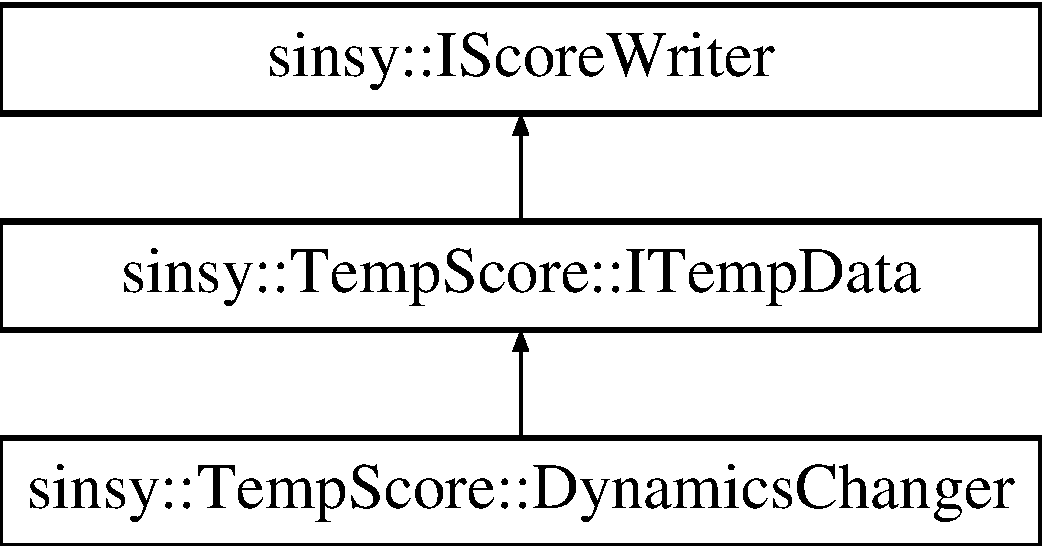
\includegraphics[height=3.000000cm]{classsinsy_1_1TempScore_1_1DynamicsChanger}
\end{center}
\end{figure}
\subsection*{\-Public \-Member \-Functions}
\begin{DoxyCompactItemize}
\item 
\hypertarget{classsinsy_1_1TempScore_1_1DynamicsChanger_ad74998ee8cf95add7660c1bf8e93dab7}{\hyperlink{classsinsy_1_1TempScore_1_1DynamicsChanger_ad74998ee8cf95add7660c1bf8e93dab7}{\-Dynamics\-Changer} (const \hyperlink{classsinsy_1_1Dynamics}{\-Dynamics} \&d)}\label{classsinsy_1_1TempScore_1_1DynamicsChanger_ad74998ee8cf95add7660c1bf8e93dab7}

\begin{DoxyCompactList}\small\item\em constructor \end{DoxyCompactList}\item 
\hypertarget{classsinsy_1_1TempScore_1_1DynamicsChanger_a073ec1a92e0b47c5139651729c3c4b82}{virtual \hyperlink{classsinsy_1_1TempScore_1_1DynamicsChanger_a073ec1a92e0b47c5139651729c3c4b82}{$\sim$\-Dynamics\-Changer} ()}\label{classsinsy_1_1TempScore_1_1DynamicsChanger_a073ec1a92e0b47c5139651729c3c4b82}

\begin{DoxyCompactList}\small\item\em destructor \end{DoxyCompactList}\item 
\hypertarget{classsinsy_1_1TempScore_1_1DynamicsChanger_ab55f77f5d4554919a2c3b76c51d8f486}{virtual void \hyperlink{classsinsy_1_1TempScore_1_1DynamicsChanger_ab55f77f5d4554919a2c3b76c51d8f486}{write} (\hyperlink{classsinsy_1_1IScoreWritable}{\-I\-Score\-Writable} \&sm) const }\label{classsinsy_1_1TempScore_1_1DynamicsChanger_ab55f77f5d4554919a2c3b76c51d8f486}

\begin{DoxyCompactList}\small\item\em write \end{DoxyCompactList}\end{DoxyCompactItemize}


\-The documentation for this class was generated from the following files\-:\begin{DoxyCompactItemize}
\item 
lib/temporary/\-Temp\-Score.\-h\item 
lib/temporary/\-Temp\-Score.\-cpp\end{DoxyCompactItemize}

\hypertarget{classsinsy_1_1TempScore_1_1EncodingSetter}{\section{sinsy\-:\-:\-Temp\-Score\-:\-:\-Encoding\-Setter \-Class \-Reference}
\label{classsinsy_1_1TempScore_1_1EncodingSetter}\index{sinsy\-::\-Temp\-Score\-::\-Encoding\-Setter@{sinsy\-::\-Temp\-Score\-::\-Encoding\-Setter}}
}
\-Inheritance diagram for sinsy\-:\-:\-Temp\-Score\-:\-:\-Encoding\-Setter\-:\begin{figure}[H]
\begin{center}
\leavevmode
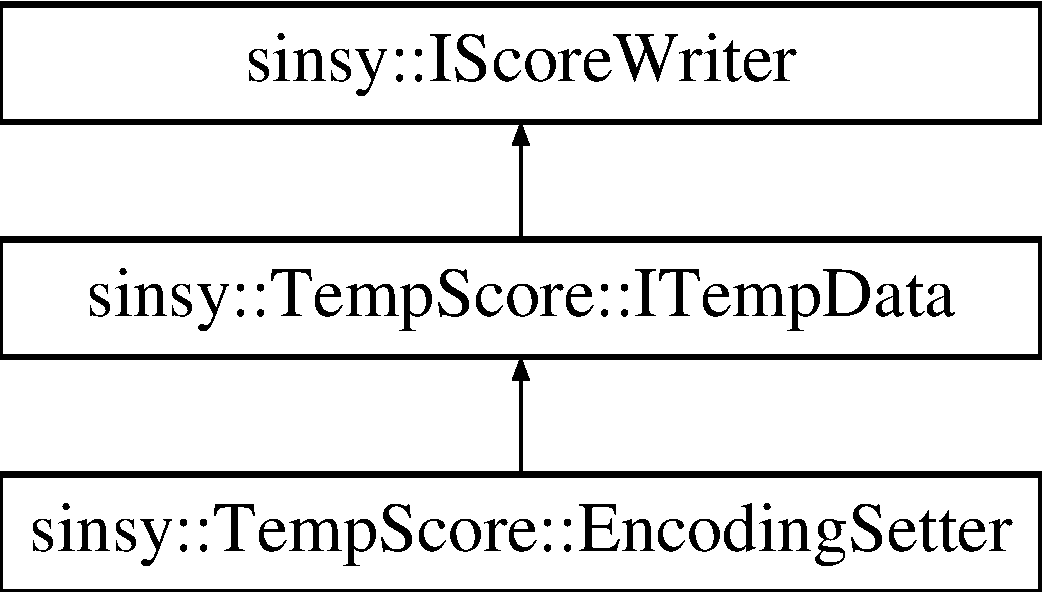
\includegraphics[height=3.000000cm]{classsinsy_1_1TempScore_1_1EncodingSetter}
\end{center}
\end{figure}
\subsection*{\-Public \-Member \-Functions}
\begin{DoxyCompactItemize}
\item 
\hypertarget{classsinsy_1_1TempScore_1_1EncodingSetter_a63a40122ab9e305eaf958f1698777877}{\hyperlink{classsinsy_1_1TempScore_1_1EncodingSetter_a63a40122ab9e305eaf958f1698777877}{\-Encoding\-Setter} (const std\-::string \&e)}\label{classsinsy_1_1TempScore_1_1EncodingSetter_a63a40122ab9e305eaf958f1698777877}

\begin{DoxyCompactList}\small\item\em constructor \end{DoxyCompactList}\item 
\hypertarget{classsinsy_1_1TempScore_1_1EncodingSetter_a63176cea655789315decbdf0c1cfc238}{virtual \hyperlink{classsinsy_1_1TempScore_1_1EncodingSetter_a63176cea655789315decbdf0c1cfc238}{$\sim$\-Encoding\-Setter} ()}\label{classsinsy_1_1TempScore_1_1EncodingSetter_a63176cea655789315decbdf0c1cfc238}

\begin{DoxyCompactList}\small\item\em destructor \end{DoxyCompactList}\item 
\hypertarget{classsinsy_1_1TempScore_1_1EncodingSetter_a92c8fea4d11bdad2efab9ef245ff5c0e}{virtual void \hyperlink{classsinsy_1_1TempScore_1_1EncodingSetter_a92c8fea4d11bdad2efab9ef245ff5c0e}{write} (\hyperlink{classsinsy_1_1IScoreWritable}{\-I\-Score\-Writable} \&sm) const }\label{classsinsy_1_1TempScore_1_1EncodingSetter_a92c8fea4d11bdad2efab9ef245ff5c0e}

\begin{DoxyCompactList}\small\item\em write \end{DoxyCompactList}\end{DoxyCompactItemize}


\-The documentation for this class was generated from the following files\-:\begin{DoxyCompactItemize}
\item 
lib/temporary/\-Temp\-Score.\-h\item 
lib/temporary/\-Temp\-Score.\-cpp\end{DoxyCompactItemize}

\hypertarget{classsinsy_1_1ForEachAdapter}{\section{sinsy\-:\-:\-For\-Each\-Adapter$<$ \-T, \-U $>$ \-Class \-Template \-Reference}
\label{classsinsy_1_1ForEachAdapter}\index{sinsy\-::\-For\-Each\-Adapter$<$ T, U $>$@{sinsy\-::\-For\-Each\-Adapter$<$ T, U $>$}}
}


{\ttfamily \#include $<$\-For\-Each\-Adapter.\-h$>$}

\subsection*{\-Public \-Types}
\begin{DoxyCompactItemize}
\item 
\hypertarget{classsinsy_1_1ForEachAdapter_ad0016aeaa71d6d5f201262e5b50b6e06}{typedef void(\-T\-::$\ast$ {\bfseries \-Func} )(\-U)}\label{classsinsy_1_1ForEachAdapter_ad0016aeaa71d6d5f201262e5b50b6e06}

\end{DoxyCompactItemize}
\subsection*{\-Public \-Member \-Functions}
\begin{DoxyCompactItemize}
\item 
\hypertarget{classsinsy_1_1ForEachAdapter_a5c6be71ea4ccfdc726ba9f9cc4f59cea}{\hyperlink{classsinsy_1_1ForEachAdapter_a5c6be71ea4ccfdc726ba9f9cc4f59cea}{\-For\-Each\-Adapter} (\-T \&o, \-Func f)}\label{classsinsy_1_1ForEachAdapter_a5c6be71ea4ccfdc726ba9f9cc4f59cea}

\begin{DoxyCompactList}\small\item\em constructor \end{DoxyCompactList}\item 
\hypertarget{classsinsy_1_1ForEachAdapter_ab01b873b14c5700101b984beb7e6017d}{virtual \hyperlink{classsinsy_1_1ForEachAdapter_ab01b873b14c5700101b984beb7e6017d}{$\sim$\-For\-Each\-Adapter} ()}\label{classsinsy_1_1ForEachAdapter_ab01b873b14c5700101b984beb7e6017d}

\begin{DoxyCompactList}\small\item\em destructor \end{DoxyCompactList}\item 
\hypertarget{classsinsy_1_1ForEachAdapter_ac2bbdd944f14ffab57c379a527c3386a}{void \hyperlink{classsinsy_1_1ForEachAdapter_ac2bbdd944f14ffab57c379a527c3386a}{operator()} (\-U u)}\label{classsinsy_1_1ForEachAdapter_ac2bbdd944f14ffab57c379a527c3386a}

\begin{DoxyCompactList}\small\item\em do function \end{DoxyCompactList}\end{DoxyCompactItemize}


\subsection{\-Detailed \-Description}
\subsubsection*{template$<$class T, class U$>$class sinsy\-::\-For\-Each\-Adapter$<$ T, U $>$}

for\-\_\-each() adapter for member function of class


\begin{DoxyParams}{\-Parameters}
{\em \-T} & class that has \-Func \\
\hline
{\em \-U} & \-: argument of \-Func \\
\hline
\end{DoxyParams}


\-The documentation for this class was generated from the following file\-:\begin{DoxyCompactItemize}
\item 
lib/util/\-For\-Each\-Adapter.\-h\end{DoxyCompactItemize}

\hypertarget{classsinsy_1_1GConf}{\section{sinsy\-:\-:\-G\-Conf \-Class \-Reference}
\label{classsinsy_1_1GConf}\index{sinsy\-::\-G\-Conf@{sinsy\-::\-G\-Conf}}
}
\-Inheritance diagram for sinsy\-:\-:\-G\-Conf\-:\begin{figure}[H]
\begin{center}
\leavevmode
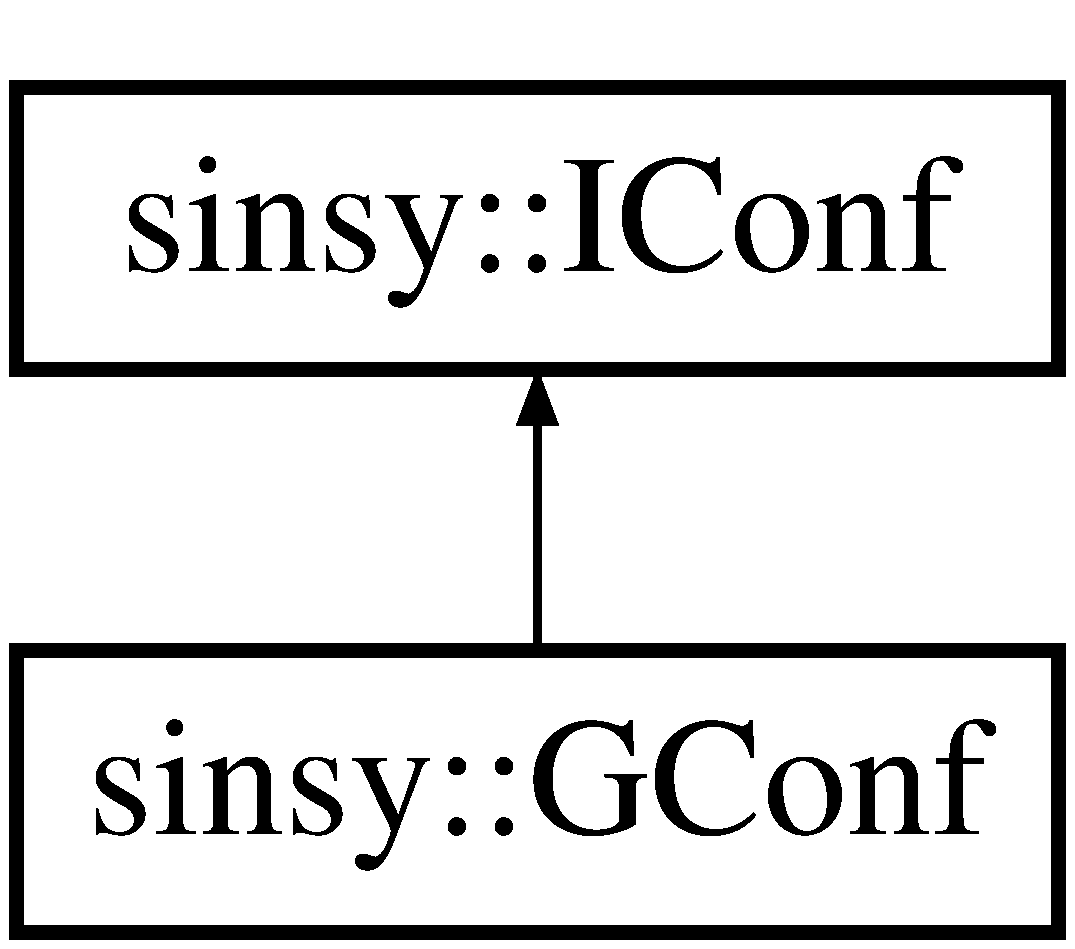
\includegraphics[height=2.000000cm]{classsinsy_1_1GConf}
\end{center}
\end{figure}
\subsection*{\-Public \-Member \-Functions}
\begin{DoxyCompactItemize}
\item 
\hypertarget{classsinsy_1_1GConf_a87bf34670529d2dc334e2aaa6fda748a}{\hyperlink{classsinsy_1_1GConf_a87bf34670529d2dc334e2aaa6fda748a}{\-G\-Conf} ()}\label{classsinsy_1_1GConf_a87bf34670529d2dc334e2aaa6fda748a}

\begin{DoxyCompactList}\small\item\em constructor \end{DoxyCompactList}\item 
\hypertarget{classsinsy_1_1GConf_af778492742a433b8f6e739e9ae55048d}{virtual \hyperlink{classsinsy_1_1GConf_af778492742a433b8f6e739e9ae55048d}{$\sim$\-G\-Conf} ()}\label{classsinsy_1_1GConf_af778492742a433b8f6e739e9ae55048d}

\begin{DoxyCompactList}\small\item\em destructor \end{DoxyCompactList}\item 
bool \hyperlink{classsinsy_1_1GConf_a6b4a07d1e386abd95d3d615e0f421e44}{convert} (const std\-::string \&enc, \-Convertable\-List\-::iterator begin, \-Convertable\-List\-::iterator end) const 
\begin{DoxyCompactList}\small\item\em convert lyrics to phonemes \end{DoxyCompactList}\item 
virtual std\-::string \hyperlink{classsinsy_1_1GConf_a0c0a0cbe05ace4e2e378bd5f82bc3bab}{get\-Sil\-Str} () const 
\begin{DoxyCompactList}\small\item\em get sil str \end{DoxyCompactList}\item 
bool \hyperlink{classsinsy_1_1GConf_a231b8129a04810396fc8cd366703c272}{read} (const std\-::string \&lexicon, const std\-::string \&phones, const std\-::string \&mapfilen)
\begin{DoxyCompactList}\small\item\em read lexicon, vowels and \-German-\/\-Japanese mapping. \-Filenames are defined in \hyperlink{GConf_8h_source}{\-G\-Conf.\-h} \end{DoxyCompactList}\item 
void \hyperlink{classsinsy_1_1GConf_aca80b35aa553ade0d65a001043bcbad4}{removechar} (std\-::string $\ast$word, char rchar)
\begin{DoxyCompactList}\small\item\em remove char from string \end{DoxyCompactList}\item 
\hypertarget{classsinsy_1_1GConf_ad6b242a11cb876dc4d971b3f3067403c}{void \hyperlink{classsinsy_1_1GConf_ad6b242a11cb876dc4d971b3f3067403c}{erasechar} (std\-::string $\ast$word, char rchar)}\label{classsinsy_1_1GConf_ad6b242a11cb876dc4d971b3f3067403c}

\begin{DoxyCompactList}\small\item\em remove char from string \end{DoxyCompactList}\end{DoxyCompactItemize}


\subsection{\-Member \-Function \-Documentation}
\hypertarget{classsinsy_1_1GConf_a6b4a07d1e386abd95d3d615e0f421e44}{\index{sinsy\-::\-G\-Conf@{sinsy\-::\-G\-Conf}!convert@{convert}}
\index{convert@{convert}!sinsy::GConf@{sinsy\-::\-G\-Conf}}
\subsubsection[{convert}]{\setlength{\rightskip}{0pt plus 5cm}bool {\bf \-G\-Conf\-::convert} (
\begin{DoxyParamCaption}
\item[{const std\-::string \&}]{enc, }
\item[{\-Convertable\-List\-::iterator}]{begin, }
\item[{\-Convertable\-List\-::iterator}]{end}
\end{DoxyParamCaption}
) const\hspace{0.3cm}{\ttfamily  \mbox{[}virtual\mbox{]}}}}\label{classsinsy_1_1GConf_a6b4a07d1e386abd95d3d615e0f421e44}


convert lyrics to phonemes 


\begin{DoxyParams}{\-Parameters}
{\em enc} & encoding \\
\hline
{\em begin} & begin of vector of \hyperlink{classsinsy_1_1IConvertable}{\-I\-Convertable} elements that have to be converted to \-German \\
\hline
{\em end} & end of the vector \\
\hline
\end{DoxyParams}
\begin{DoxyReturn}{\-Returns}
true if success 
\end{DoxyReturn}


\-Implements \hyperlink{classsinsy_1_1IConf_a892ad5cc8098a0b2bb720deade6dc0ee}{sinsy\-::\-I\-Conf}.

\hypertarget{classsinsy_1_1GConf_a0c0a0cbe05ace4e2e378bd5f82bc3bab}{\index{sinsy\-::\-G\-Conf@{sinsy\-::\-G\-Conf}!get\-Sil\-Str@{get\-Sil\-Str}}
\index{get\-Sil\-Str@{get\-Sil\-Str}!sinsy::GConf@{sinsy\-::\-G\-Conf}}
\subsubsection[{get\-Sil\-Str}]{\setlength{\rightskip}{0pt plus 5cm}std\-::string {\bf \-G\-Conf\-::get\-Sil\-Str} (
\begin{DoxyParamCaption}
{}
\end{DoxyParamCaption}
) const\hspace{0.3cm}{\ttfamily  \mbox{[}virtual\mbox{]}}}}\label{classsinsy_1_1GConf_a0c0a0cbe05ace4e2e378bd5f82bc3bab}


get sil str 

return sil str 

\-Implements \hyperlink{classsinsy_1_1IConf_a6b4b753e87291960ccc88867d97ef280}{sinsy\-::\-I\-Conf}.

\hypertarget{classsinsy_1_1GConf_a231b8129a04810396fc8cd366703c272}{\index{sinsy\-::\-G\-Conf@{sinsy\-::\-G\-Conf}!read@{read}}
\index{read@{read}!sinsy::GConf@{sinsy\-::\-G\-Conf}}
\subsubsection[{read}]{\setlength{\rightskip}{0pt plus 5cm}bool {\bf \-G\-Conf\-::read} (
\begin{DoxyParamCaption}
\item[{const std\-::string \&}]{lexiconn, }
\item[{const std\-::string \&}]{vowelsn, }
\item[{const std\-::string \&}]{mapfilen}
\end{DoxyParamCaption}
)}}\label{classsinsy_1_1GConf_a231b8129a04810396fc8cd366703c272}


read lexicon, vowels and \-German-\/\-Japanese mapping. \-Filenames are defined in \hyperlink{GConf_8h_source}{\-G\-Conf.\-h} 


\begin{DoxyParams}{\-Parameters}
{\em lexiconn} & name of lexicon file \\
\hline
{\em vowelsn} & name of vowels file \\
\hline
{\em mapfilen} & mapping between \-German and \-Japanese vowels \\
\hline
\end{DoxyParams}
\begin{DoxyReturn}{\-Returns}
true if success 
\end{DoxyReturn}
\hypertarget{classsinsy_1_1GConf_aca80b35aa553ade0d65a001043bcbad4}{\index{sinsy\-::\-G\-Conf@{sinsy\-::\-G\-Conf}!removechar@{removechar}}
\index{removechar@{removechar}!sinsy::GConf@{sinsy\-::\-G\-Conf}}
\subsubsection[{removechar}]{\setlength{\rightskip}{0pt plus 5cm}void {\bf \-G\-Conf\-::removechar} (
\begin{DoxyParamCaption}
\item[{std\-::string $\ast$}]{word, }
\item[{char}]{rchar}
\end{DoxyParamCaption}
)}}\label{classsinsy_1_1GConf_aca80b35aa553ade0d65a001043bcbad4}


remove char from string 


\begin{DoxyParams}{\-Parameters}
{\em word} & string to remove from \\
\hline
{\em rchar} & char to remvoe \\
\hline
\end{DoxyParams}


\-The documentation for this class was generated from the following files\-:\begin{DoxyCompactItemize}
\item 
lib/german/\-G\-Conf.\-h\item 
lib/german/\-G\-Conf.\-cpp\end{DoxyCompactItemize}

\hypertarget{classsinsy_1_1HtsEngine}{\section{sinsy\-:\-:\-Hts\-Engine \-Class \-Reference}
\label{classsinsy_1_1HtsEngine}\index{sinsy\-::\-Hts\-Engine@{sinsy\-::\-Hts\-Engine}}
}
\subsection*{\-Public \-Member \-Functions}
\begin{DoxyCompactItemize}
\item 
\hypertarget{classsinsy_1_1HtsEngine_abc60230d1bb17390cac5208ad92a7f1f}{\hyperlink{classsinsy_1_1HtsEngine_abc60230d1bb17390cac5208ad92a7f1f}{\-Hts\-Engine} ()}\label{classsinsy_1_1HtsEngine_abc60230d1bb17390cac5208ad92a7f1f}

\begin{DoxyCompactList}\small\item\em constructor \end{DoxyCompactList}\item 
\hypertarget{classsinsy_1_1HtsEngine_a9d9afbaddb75474cf4ffe33654579295}{virtual \hyperlink{classsinsy_1_1HtsEngine_a9d9afbaddb75474cf4ffe33654579295}{$\sim$\-Hts\-Engine} ()}\label{classsinsy_1_1HtsEngine_a9d9afbaddb75474cf4ffe33654579295}

\begin{DoxyCompactList}\small\item\em destructor \end{DoxyCompactList}\item 
\hypertarget{classsinsy_1_1HtsEngine_a337a3979d17c2fcd2414a41b02945fac}{void \hyperlink{classsinsy_1_1HtsEngine_a337a3979d17c2fcd2414a41b02945fac}{reset} ()}\label{classsinsy_1_1HtsEngine_a337a3979d17c2fcd2414a41b02945fac}

\begin{DoxyCompactList}\small\item\em reset \end{DoxyCompactList}\item 
\hypertarget{classsinsy_1_1HtsEngine_a05a749ae2088408c428f7a06c52bc353}{bool \hyperlink{classsinsy_1_1HtsEngine_a05a749ae2088408c428f7a06c52bc353}{load} (const std\-::vector$<$ std\-::string $>$ \&)}\label{classsinsy_1_1HtsEngine_a05a749ae2088408c428f7a06c52bc353}

\begin{DoxyCompactList}\small\item\em load voices \end{DoxyCompactList}\item 
\hypertarget{classsinsy_1_1HtsEngine_acb65581494d993aaa5009a766b3be8b5}{bool \hyperlink{classsinsy_1_1HtsEngine_acb65581494d993aaa5009a766b3be8b5}{synthesize} (const \hyperlink{classsinsy_1_1LabelStrings}{\-Label\-Strings} \&label, \hyperlink{classsinsy_1_1SynthConditionImpl}{\-Synth\-Condition\-Impl} \&condition)}\label{classsinsy_1_1HtsEngine_acb65581494d993aaa5009a766b3be8b5}

\begin{DoxyCompactList}\small\item\em synthesize \end{DoxyCompactList}\item 
void \hyperlink{classsinsy_1_1HtsEngine_aeaff234f779eac7bc3b1d8de08c9914c}{stop} ()
\begin{DoxyCompactList}\small\item\em stop synthesizing \end{DoxyCompactList}\item 
\hypertarget{classsinsy_1_1HtsEngine_a9d8591f35e699329909ca73a458122e9}{void \hyperlink{classsinsy_1_1HtsEngine_a9d8591f35e699329909ca73a458122e9}{reset\-Stop\-Flag} ()}\label{classsinsy_1_1HtsEngine_a9d8591f35e699329909ca73a458122e9}

\begin{DoxyCompactList}\small\item\em reset stop flag \end{DoxyCompactList}\item 
\hypertarget{classsinsy_1_1HtsEngine_adc092679d64b638c9ae642377b1a6cd1}{bool \hyperlink{classsinsy_1_1HtsEngine_adc092679d64b638c9ae642377b1a6cd1}{set\-Alpha} (double)}\label{classsinsy_1_1HtsEngine_adc092679d64b638c9ae642377b1a6cd1}

\begin{DoxyCompactList}\small\item\em set alpha \end{DoxyCompactList}\item 
\hypertarget{classsinsy_1_1HtsEngine_a8e56a7f848e852a44bfd52cbb61042ec}{bool \hyperlink{classsinsy_1_1HtsEngine_a8e56a7f848e852a44bfd52cbb61042ec}{set\-Tone} (double)}\label{classsinsy_1_1HtsEngine_a8e56a7f848e852a44bfd52cbb61042ec}

\begin{DoxyCompactList}\small\item\em set tone \end{DoxyCompactList}\item 
\hypertarget{classsinsy_1_1HtsEngine_adf65be063e9eba483ad2da588151903f}{bool \hyperlink{classsinsy_1_1HtsEngine_adf65be063e9eba483ad2da588151903f}{set\-Speed} (double)}\label{classsinsy_1_1HtsEngine_adf65be063e9eba483ad2da588151903f}

\begin{DoxyCompactList}\small\item\em set speed \end{DoxyCompactList}\item 
\hypertarget{classsinsy_1_1HtsEngine_a904a3fb6b61aa7ae0d101db4b38b1045}{bool \hyperlink{classsinsy_1_1HtsEngine_a904a3fb6b61aa7ae0d101db4b38b1045}{set\-Volume} (double)}\label{classsinsy_1_1HtsEngine_a904a3fb6b61aa7ae0d101db4b38b1045}

\begin{DoxyCompactList}\small\item\em set volume \end{DoxyCompactList}\item 
\hypertarget{classsinsy_1_1HtsEngine_a2d042c805e8645e135a7954f933fe6bf}{bool \hyperlink{classsinsy_1_1HtsEngine_a2d042c805e8645e135a7954f933fe6bf}{set\-Interpolation\-Weight} (size\-\_\-t, double)}\label{classsinsy_1_1HtsEngine_a2d042c805e8645e135a7954f933fe6bf}

\begin{DoxyCompactList}\small\item\em set interpolation weight \end{DoxyCompactList}\end{DoxyCompactItemize}


\subsection{\-Member \-Function \-Documentation}
\hypertarget{classsinsy_1_1HtsEngine_aeaff234f779eac7bc3b1d8de08c9914c}{\index{sinsy\-::\-Hts\-Engine@{sinsy\-::\-Hts\-Engine}!stop@{stop}}
\index{stop@{stop}!sinsy::HtsEngine@{sinsy\-::\-Hts\-Engine}}
\subsubsection[{stop}]{\setlength{\rightskip}{0pt plus 5cm}void {\bf \-Hts\-Engine\-::stop} (
\begin{DoxyParamCaption}
{}
\end{DoxyParamCaption}
)}}\label{classsinsy_1_1HtsEngine_aeaff234f779eac7bc3b1d8de08c9914c}


stop synthesizing 

stop 

\-The documentation for this class was generated from the following files\-:\begin{DoxyCompactItemize}
\item 
lib/hts\-\_\-engine\-\_\-\-A\-P\-I/\-Hts\-Engine.\-h\item 
lib/hts\-\_\-engine\-\_\-\-A\-P\-I/\-Hts\-Engine.\-cpp\end{DoxyCompactItemize}

\hypertarget{classsinsy_1_1IConf}{\section{sinsy\-:\-:\-I\-Conf \-Class \-Reference}
\label{classsinsy_1_1IConf}\index{sinsy\-::\-I\-Conf@{sinsy\-::\-I\-Conf}}
}
\-Inheritance diagram for sinsy\-:\-:\-I\-Conf\-:\begin{figure}[H]
\begin{center}
\leavevmode
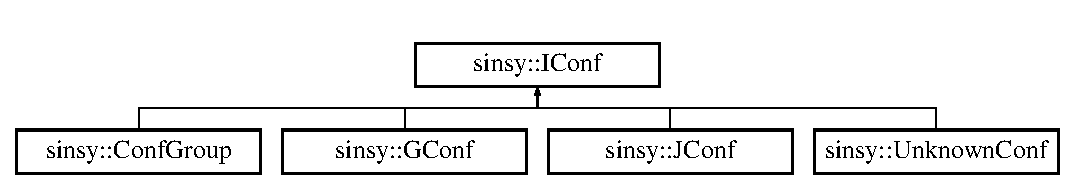
\includegraphics[height=2.000000cm]{classsinsy_1_1IConf}
\end{center}
\end{figure}
\subsection*{\-Public \-Types}
\begin{DoxyCompactItemize}
\item 
\hypertarget{classsinsy_1_1IConf_aef94406d617b334239fd77ed2e152517}{typedef std\-::vector\*
$<$ \hyperlink{classsinsy_1_1IConvertable}{\-I\-Convertable} $\ast$ $>$ {\bfseries \-Convertable\-List}}\label{classsinsy_1_1IConf_aef94406d617b334239fd77ed2e152517}

\end{DoxyCompactItemize}
\subsection*{\-Public \-Member \-Functions}
\begin{DoxyCompactItemize}
\item 
\hypertarget{classsinsy_1_1IConf_a1475838222465dda71482db6b745602c}{virtual \hyperlink{classsinsy_1_1IConf_a1475838222465dda71482db6b745602c}{$\sim$\-I\-Conf} ()}\label{classsinsy_1_1IConf_a1475838222465dda71482db6b745602c}

\begin{DoxyCompactList}\small\item\em destructor \end{DoxyCompactList}\item 
\hypertarget{classsinsy_1_1IConf_a892ad5cc8098a0b2bb720deade6dc0ee}{virtual bool \hyperlink{classsinsy_1_1IConf_a892ad5cc8098a0b2bb720deade6dc0ee}{convert} (const std\-::string \&enc, \-Convertable\-List\-::iterator begin, \-Convertable\-List\-::iterator end) const =0}\label{classsinsy_1_1IConf_a892ad5cc8098a0b2bb720deade6dc0ee}

\begin{DoxyCompactList}\small\item\em convert \end{DoxyCompactList}\item 
\hypertarget{classsinsy_1_1IConf_a6b4b753e87291960ccc88867d97ef280}{virtual std\-::string \hyperlink{classsinsy_1_1IConf_a6b4b753e87291960ccc88867d97ef280}{get\-Sil\-Str} () const =0}\label{classsinsy_1_1IConf_a6b4b753e87291960ccc88867d97ef280}

\begin{DoxyCompactList}\small\item\em get sil string \end{DoxyCompactList}\end{DoxyCompactItemize}


\-The documentation for this class was generated from the following file\-:\begin{DoxyCompactItemize}
\item 
lib/converter/\-I\-Conf.\-h\end{DoxyCompactItemize}

\hypertarget{classsinsy_1_1IConvertable}{\section{sinsy\-:\-:\-I\-Convertable \-Class \-Reference}
\label{classsinsy_1_1IConvertable}\index{sinsy\-::\-I\-Convertable@{sinsy\-::\-I\-Convertable}}
}
\-Inheritance diagram for sinsy\-:\-:\-I\-Convertable\-:\begin{figure}[H]
\begin{center}
\leavevmode
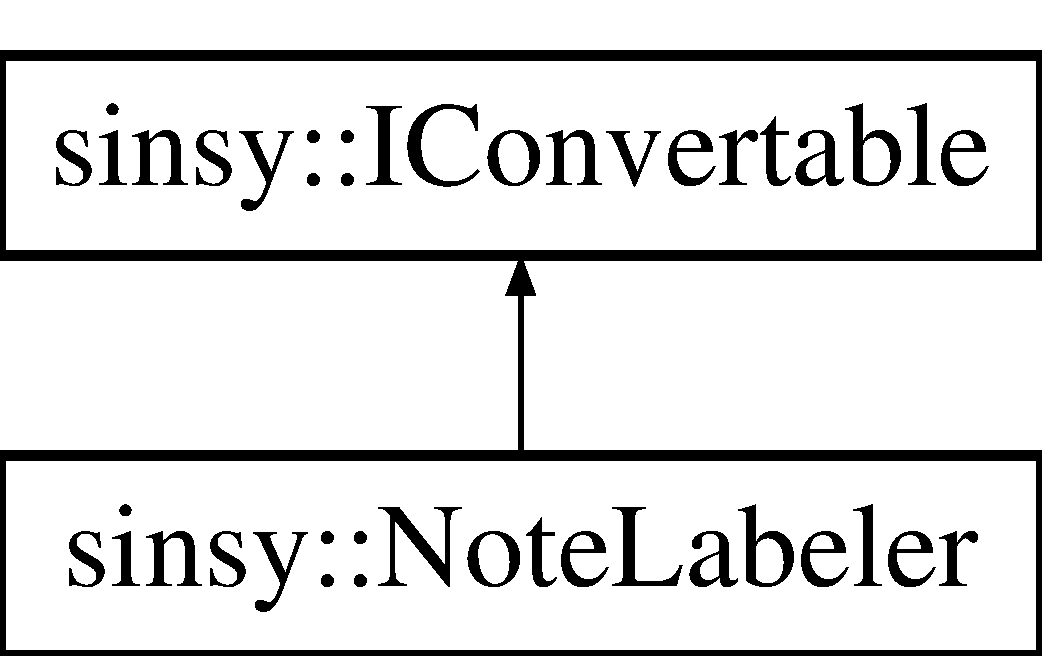
\includegraphics[height=2.000000cm]{classsinsy_1_1IConvertable}
\end{center}
\end{figure}
\subsection*{\-Public \-Member \-Functions}
\begin{DoxyCompactItemize}
\item 
\hypertarget{classsinsy_1_1IConvertable_ab66b261751f1e6843d5b7fc455b28ad6}{virtual \hyperlink{classsinsy_1_1IConvertable_ab66b261751f1e6843d5b7fc455b28ad6}{$\sim$\-I\-Convertable} ()}\label{classsinsy_1_1IConvertable_ab66b261751f1e6843d5b7fc455b28ad6}

\begin{DoxyCompactList}\small\item\em destructor \end{DoxyCompactList}\item 
\hypertarget{classsinsy_1_1IConvertable_a04aad16eb0150451a0265f07b6668c11}{virtual bool \hyperlink{classsinsy_1_1IConvertable_a04aad16eb0150451a0265f07b6668c11}{is\-Rest} () const =0}\label{classsinsy_1_1IConvertable_a04aad16eb0150451a0265f07b6668c11}

\begin{DoxyCompactList}\small\item\em \-If this is a rest, return true. \end{DoxyCompactList}\item 
\hypertarget{classsinsy_1_1IConvertable_a381d85f5055f01b7468f0541701e9b1f}{virtual bool \hyperlink{classsinsy_1_1IConvertable_a381d85f5055f01b7468f0541701e9b1f}{is\-Converted} () const =0}\label{classsinsy_1_1IConvertable_a381d85f5055f01b7468f0541701e9b1f}

\begin{DoxyCompactList}\small\item\em \-If this is already converted, return true. \end{DoxyCompactList}\item 
\hypertarget{classsinsy_1_1IConvertable_ab3bc6bf5cf525605844d2f9b3635d30d}{virtual std\-::string \hyperlink{classsinsy_1_1IConvertable_ab3bc6bf5cf525605844d2f9b3635d30d}{get\-Lyric} () const =0}\label{classsinsy_1_1IConvertable_ab3bc6bf5cf525605844d2f9b3635d30d}

\begin{DoxyCompactList}\small\item\em get lyric \end{DoxyCompactList}\item 
\hypertarget{classsinsy_1_1IConvertable_ad4df340bc95b0af3003b680eee25ed0d}{virtual \hyperlink{classsinsy_1_1Syllabic}{\-Syllabic} \hyperlink{classsinsy_1_1IConvertable_ad4df340bc95b0af3003b680eee25ed0d}{get\-Syllabic} () const =0}\label{classsinsy_1_1IConvertable_ad4df340bc95b0af3003b680eee25ed0d}

\begin{DoxyCompactList}\small\item\em get syllabic \end{DoxyCompactList}\item 
\hypertarget{classsinsy_1_1IConvertable_ae0326517f226fc7f569b5886084d6135}{virtual void \hyperlink{classsinsy_1_1IConvertable_ae0326517f226fc7f569b5886084d6135}{add\-Info} (const std\-::vector$<$ \hyperlink{classsinsy_1_1PhonemeInfo}{\-Phoneme\-Info} $>$ \&phonemes, const std\-::string \&language=\char`\"{}\char`\"{}, const std\-::string \&info=\char`\"{}\char`\"{})=0}\label{classsinsy_1_1IConvertable_ae0326517f226fc7f569b5886084d6135}

\begin{DoxyCompactList}\small\item\em add info (lyric, phonemes, and so on...) \end{DoxyCompactList}\end{DoxyCompactItemize}


\-The documentation for this class was generated from the following file\-:\begin{DoxyCompactItemize}
\item 
lib/converter/\-I\-Convertable.\-h\end{DoxyCompactItemize}

\hypertarget{classsinsy_1_1ILabelOutput}{\section{sinsy\-:\-:\-I\-Label\-Output \-Class \-Reference}
\label{classsinsy_1_1ILabelOutput}\index{sinsy\-::\-I\-Label\-Output@{sinsy\-::\-I\-Label\-Output}}
}
\-Inheritance diagram for sinsy\-:\-:\-I\-Label\-Output\-:\begin{figure}[H]
\begin{center}
\leavevmode
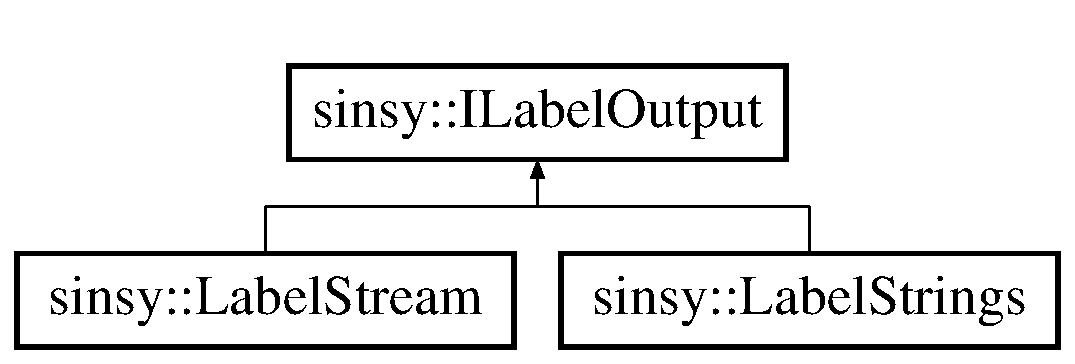
\includegraphics[height=2.000000cm]{classsinsy_1_1ILabelOutput}
\end{center}
\end{figure}
\subsection*{\-Public \-Member \-Functions}
\begin{DoxyCompactItemize}
\item 
\hypertarget{classsinsy_1_1ILabelOutput_a1b5605af046ca405ce143943614cca0e}{virtual \hyperlink{classsinsy_1_1ILabelOutput_a1b5605af046ca405ce143943614cca0e}{$\sim$\-I\-Label\-Output} ()}\label{classsinsy_1_1ILabelOutput_a1b5605af046ca405ce143943614cca0e}

\begin{DoxyCompactList}\small\item\em destructor \end{DoxyCompactList}\item 
\hypertarget{classsinsy_1_1ILabelOutput_a5ba6152a812e466398a45db0106a11bb}{virtual void \hyperlink{classsinsy_1_1ILabelOutput_a5ba6152a812e466398a45db0106a11bb}{output} (const std\-::string \&str)=0}\label{classsinsy_1_1ILabelOutput_a5ba6152a812e466398a45db0106a11bb}

\begin{DoxyCompactList}\small\item\em output \end{DoxyCompactList}\end{DoxyCompactItemize}


\-The documentation for this class was generated from the following file\-:\begin{DoxyCompactItemize}
\item 
lib/label/\-I\-Label\-Output.\-h\end{DoxyCompactItemize}

\hypertarget{classsinsy_1_1INoteLabel}{\section{sinsy\-:\-:\-I\-Note\-Label \-Class \-Reference}
\label{classsinsy_1_1INoteLabel}\index{sinsy\-::\-I\-Note\-Label@{sinsy\-::\-I\-Note\-Label}}
}
\subsection*{\-Public \-Member \-Functions}
\begin{DoxyCompactItemize}
\item 
\hypertarget{classsinsy_1_1INoteLabel_a1b0809a1b7961bb200ede93de24c1d4a}{virtual \hyperlink{classsinsy_1_1INoteLabel_a1b0809a1b7961bb200ede93de24c1d4a}{$\sim$\-I\-Note\-Label} ()}\label{classsinsy_1_1INoteLabel_a1b0809a1b7961bb200ede93de24c1d4a}

\begin{DoxyCompactList}\small\item\em destructor \end{DoxyCompactList}\item 
\hypertarget{classsinsy_1_1INoteLabel_a245d872cc6225c8e8176d6f4eb07a32e}{virtual void \hyperlink{classsinsy_1_1INoteLabel_a245d872cc6225c8e8176d6f4eb07a32e}{set\-Absolute\-Pitch} (const \hyperlink{classsinsy_1_1Pitch}{\-Pitch} \&)=0}\label{classsinsy_1_1INoteLabel_a245d872cc6225c8e8176d6f4eb07a32e}

\begin{DoxyCompactList}\small\item\em set absolute pitch \end{DoxyCompactList}\item 
\hypertarget{classsinsy_1_1INoteLabel_a5e12bcb18180fea22c79c7a4ce515e2e}{virtual void \hyperlink{classsinsy_1_1INoteLabel_a5e12bcb18180fea22c79c7a4ce515e2e}{set\-Relative\-Pitch} (size\-\_\-t)=0}\label{classsinsy_1_1INoteLabel_a5e12bcb18180fea22c79c7a4ce515e2e}

\begin{DoxyCompactList}\small\item\em set relative pitch \end{DoxyCompactList}\item 
\hypertarget{classsinsy_1_1INoteLabel_a235457769dacc677f9107a0d0154a100}{virtual void \hyperlink{classsinsy_1_1INoteLabel_a235457769dacc677f9107a0d0154a100}{set\-Key} (size\-\_\-t)=0}\label{classsinsy_1_1INoteLabel_a235457769dacc677f9107a0d0154a100}

\begin{DoxyCompactList}\small\item\em set key \end{DoxyCompactList}\item 
\hypertarget{classsinsy_1_1INoteLabel_a042fc3831e75f82aaa260e6f9ad6c420}{virtual void \hyperlink{classsinsy_1_1INoteLabel_a042fc3831e75f82aaa260e6f9ad6c420}{set\-Beat} (const \hyperlink{classsinsy_1_1Beat}{\-Beat} \&)=0}\label{classsinsy_1_1INoteLabel_a042fc3831e75f82aaa260e6f9ad6c420}

\begin{DoxyCompactList}\small\item\em set beat \end{DoxyCompactList}\item 
\hypertarget{classsinsy_1_1INoteLabel_aa1b79ffb63d27774b83edc04b92ae26b}{virtual void \hyperlink{classsinsy_1_1INoteLabel_aa1b79ffb63d27774b83edc04b92ae26b}{set\-Tempo} (double)=0}\label{classsinsy_1_1INoteLabel_aa1b79ffb63d27774b83edc04b92ae26b}

\begin{DoxyCompactList}\small\item\em set tempo \end{DoxyCompactList}\item 
\hypertarget{classsinsy_1_1INoteLabel_a5bb9bbf4bb64d341860701cec20faae7}{virtual void \hyperlink{classsinsy_1_1INoteLabel_a5bb9bbf4bb64d341860701cec20faae7}{set\-Syllable\-Num} (size\-\_\-t)=0}\label{classsinsy_1_1INoteLabel_a5bb9bbf4bb64d341860701cec20faae7}

\begin{DoxyCompactList}\small\item\em set number of syllables \end{DoxyCompactList}\item 
\hypertarget{classsinsy_1_1INoteLabel_aa58f64fff29825e61f7bb6b8019a84bb}{virtual void \hyperlink{classsinsy_1_1INoteLabel_aa58f64fff29825e61f7bb6b8019a84bb}{set\-Length} (const \hyperlink{classsinsy_1_1LabelPosition}{\-Label\-Position} \&)=0}\label{classsinsy_1_1INoteLabel_aa58f64fff29825e61f7bb6b8019a84bb}

\begin{DoxyCompactList}\small\item\em set length \end{DoxyCompactList}\item 
\hypertarget{classsinsy_1_1INoteLabel_a427c50d1287a56bd349239d17ed92caa}{virtual void \hyperlink{classsinsy_1_1INoteLabel_a427c50d1287a56bd349239d17ed92caa}{set\-Position\-In\-Measure} (const \hyperlink{classsinsy_1_1LabelPosition}{\-Label\-Position} \&, const \hyperlink{classsinsy_1_1LabelPosition}{\-Label\-Position} \&)=0}\label{classsinsy_1_1INoteLabel_a427c50d1287a56bd349239d17ed92caa}

\begin{DoxyCompactList}\small\item\em set position in measure \end{DoxyCompactList}\item 
\hypertarget{classsinsy_1_1INoteLabel_a5e81fedeba366969f4a31eb3ae775289}{virtual void \hyperlink{classsinsy_1_1INoteLabel_a5e81fedeba366969f4a31eb3ae775289}{set\-Position\-In\-Phrase} (const \hyperlink{classsinsy_1_1LabelPosition}{\-Label\-Position} \&, const \hyperlink{classsinsy_1_1LabelPosition}{\-Label\-Position} \&)=0}\label{classsinsy_1_1INoteLabel_a5e81fedeba366969f4a31eb3ae775289}

\begin{DoxyCompactList}\small\item\em set position in phrase \end{DoxyCompactList}\item 
\hypertarget{classsinsy_1_1INoteLabel_a4d6d95388916cea8c4fa7646dcc5dc4c}{virtual void \hyperlink{classsinsy_1_1INoteLabel_a4d6d95388916cea8c4fa7646dcc5dc4c}{set\-Slur\-From\-Prev} (bool)=0}\label{classsinsy_1_1INoteLabel_a4d6d95388916cea8c4fa7646dcc5dc4c}

\begin{DoxyCompactList}\small\item\em set slur from previous note \end{DoxyCompactList}\item 
\hypertarget{classsinsy_1_1INoteLabel_ab9619cc498ff3ddb2cc9a310a4fbddd4}{virtual void \hyperlink{classsinsy_1_1INoteLabel_ab9619cc498ff3ddb2cc9a310a4fbddd4}{set\-Slur\-To\-Next} (bool)=0}\label{classsinsy_1_1INoteLabel_ab9619cc498ff3ddb2cc9a310a4fbddd4}

\begin{DoxyCompactList}\small\item\em set slur to next note \end{DoxyCompactList}\item 
\hypertarget{classsinsy_1_1INoteLabel_a2a0c5043698dd60c1b9ea448d6ce39e8}{virtual void \hyperlink{classsinsy_1_1INoteLabel_a2a0c5043698dd60c1b9ea448d6ce39e8}{set\-Dynamics} (const \hyperlink{classsinsy_1_1Dynamics}{\-Dynamics} \&)=0}\label{classsinsy_1_1INoteLabel_a2a0c5043698dd60c1b9ea448d6ce39e8}

\begin{DoxyCompactList}\small\item\em set dynamics \end{DoxyCompactList}\item 
\hypertarget{classsinsy_1_1INoteLabel_ac8726aec10e115e6c33ea9b758ac120c}{virtual void \hyperlink{classsinsy_1_1INoteLabel_ac8726aec10e115e6c33ea9b758ac120c}{set\-Length\-From\-Prev\-Accent} (const \hyperlink{classsinsy_1_1LabelPosition}{\-Label\-Position} \&)=0}\label{classsinsy_1_1INoteLabel_ac8726aec10e115e6c33ea9b758ac120c}

\begin{DoxyCompactList}\small\item\em set length from previous accent \end{DoxyCompactList}\item 
\hypertarget{classsinsy_1_1INoteLabel_aeef956ffef5e64d64ed1b6005561755f}{virtual void \hyperlink{classsinsy_1_1INoteLabel_aeef956ffef5e64d64ed1b6005561755f}{set\-Length\-To\-Next\-Accent} (const \hyperlink{classsinsy_1_1LabelPosition}{\-Label\-Position} \&)=0}\label{classsinsy_1_1INoteLabel_aeef956ffef5e64d64ed1b6005561755f}

\begin{DoxyCompactList}\small\item\em set length to next accent \end{DoxyCompactList}\item 
\hypertarget{classsinsy_1_1INoteLabel_a6858fae4cc676d1a54fe6f7b7b7d00c5}{virtual void \hyperlink{classsinsy_1_1INoteLabel_a6858fae4cc676d1a54fe6f7b7b7d00c5}{set\-Length\-From\-Prev\-Staccato} (const \hyperlink{classsinsy_1_1LabelPosition}{\-Label\-Position} \&)=0}\label{classsinsy_1_1INoteLabel_a6858fae4cc676d1a54fe6f7b7b7d00c5}

\begin{DoxyCompactList}\small\item\em set length from previous staccato \end{DoxyCompactList}\item 
\hypertarget{classsinsy_1_1INoteLabel_ac34fd47e368de626f60fb320e229de13}{virtual void \hyperlink{classsinsy_1_1INoteLabel_ac34fd47e368de626f60fb320e229de13}{set\-Length\-To\-Next\-Staccato} (const \hyperlink{classsinsy_1_1LabelPosition}{\-Label\-Position} \&)=0}\label{classsinsy_1_1INoteLabel_ac34fd47e368de626f60fb320e229de13}

\begin{DoxyCompactList}\small\item\em set length to next staccato \end{DoxyCompactList}\item 
\hypertarget{classsinsy_1_1INoteLabel_aac7080ee06a8d7042a1e2aa65130a758}{virtual void \hyperlink{classsinsy_1_1INoteLabel_aac7080ee06a8d7042a1e2aa65130a758}{set\-Position\-In\-Crescendo} (const \hyperlink{classsinsy_1_1LabelPosition}{\-Label\-Position} \&, const \hyperlink{classsinsy_1_1LabelPosition}{\-Label\-Position} \&)=0}\label{classsinsy_1_1INoteLabel_aac7080ee06a8d7042a1e2aa65130a758}

\begin{DoxyCompactList}\small\item\em set position in crescendo \end{DoxyCompactList}\item 
\hypertarget{classsinsy_1_1INoteLabel_ad31fbf650c2d5a146bb0eea67b864694}{virtual void \hyperlink{classsinsy_1_1INoteLabel_ad31fbf650c2d5a146bb0eea67b864694}{set\-Position\-In\-Diminuendo} (const \hyperlink{classsinsy_1_1LabelPosition}{\-Label\-Position} \&, const \hyperlink{classsinsy_1_1LabelPosition}{\-Label\-Position} \&)=0}\label{classsinsy_1_1INoteLabel_ad31fbf650c2d5a146bb0eea67b864694}

\begin{DoxyCompactList}\small\item\em set position in diminuendo \end{DoxyCompactList}\item 
\hypertarget{classsinsy_1_1INoteLabel_ad06342db34abe89d5ef26ab8970b2656}{virtual void \hyperlink{classsinsy_1_1INoteLabel_ad06342db34abe89d5ef26ab8970b2656}{set\-Pitch\-Difference\-From\-Prev} (int)=0}\label{classsinsy_1_1INoteLabel_ad06342db34abe89d5ef26ab8970b2656}

\begin{DoxyCompactList}\small\item\em set pitch difference from previous note \end{DoxyCompactList}\item 
\hypertarget{classsinsy_1_1INoteLabel_a1484fd3652fcee6b9e6859776391b36d}{virtual void \hyperlink{classsinsy_1_1INoteLabel_a1484fd3652fcee6b9e6859776391b36d}{set\-Pitch\-Difference\-To\-Next} (int)=0}\label{classsinsy_1_1INoteLabel_a1484fd3652fcee6b9e6859776391b36d}

\begin{DoxyCompactList}\small\item\em set pitch difference to next note \end{DoxyCompactList}\item 
\hypertarget{classsinsy_1_1INoteLabel_acc711c4d7e793b8b4d8d68af60b58d8d}{virtual void \hyperlink{classsinsy_1_1INoteLabel_acc711c4d7e793b8b4d8d68af60b58d8d}{set\-Breath\-From\-Prev} (bool)=0}\label{classsinsy_1_1INoteLabel_acc711c4d7e793b8b4d8d68af60b58d8d}

\begin{DoxyCompactList}\small\item\em set breath between previous and this notes \end{DoxyCompactList}\item 
\hypertarget{classsinsy_1_1INoteLabel_a8909de491adc0b26c6a92d20676b903e}{virtual void \hyperlink{classsinsy_1_1INoteLabel_a8909de491adc0b26c6a92d20676b903e}{set\-Breath\-To\-Next} (bool)=0}\label{classsinsy_1_1INoteLabel_a8909de491adc0b26c6a92d20676b903e}

\begin{DoxyCompactList}\small\item\em set breath between this and next notes \end{DoxyCompactList}\item 
\hypertarget{classsinsy_1_1INoteLabel_a2da3a8c3126f624ebb8a97695f8bf4cb}{virtual void \hyperlink{classsinsy_1_1INoteLabel_a2da3a8c3126f624ebb8a97695f8bf4cb}{set\-Prev\-Phrase\-Info} (size\-\_\-t, size\-\_\-t)=0}\label{classsinsy_1_1INoteLabel_a2da3a8c3126f624ebb8a97695f8bf4cb}

\begin{DoxyCompactList}\small\item\em set previous phrase info \end{DoxyCompactList}\item 
\hypertarget{classsinsy_1_1INoteLabel_acbc3eab9267025b6a62a0d5d76ec7c65}{virtual void \hyperlink{classsinsy_1_1INoteLabel_acbc3eab9267025b6a62a0d5d76ec7c65}{set\-Phrase\-Info} (size\-\_\-t, size\-\_\-t)=0}\label{classsinsy_1_1INoteLabel_acbc3eab9267025b6a62a0d5d76ec7c65}

\begin{DoxyCompactList}\small\item\em set phrase info \end{DoxyCompactList}\item 
\hypertarget{classsinsy_1_1INoteLabel_aa2cb2cba5f212ec43e1043987260eed8}{virtual void \hyperlink{classsinsy_1_1INoteLabel_aa2cb2cba5f212ec43e1043987260eed8}{set\-Next\-Phrase\-Info} (size\-\_\-t, size\-\_\-t)=0}\label{classsinsy_1_1INoteLabel_aa2cb2cba5f212ec43e1043987260eed8}

\begin{DoxyCompactList}\small\item\em set next phrase info \end{DoxyCompactList}\end{DoxyCompactItemize}


\-The documentation for this class was generated from the following file\-:\begin{DoxyCompactItemize}
\item 
lib/label/\-I\-Note\-Label.\-h\end{DoxyCompactItemize}

\hypertarget{classsinsy_1_1InputFile}{\section{sinsy\-:\-:\-Input\-File \-Class \-Reference}
\label{classsinsy_1_1InputFile}\index{sinsy\-::\-Input\-File@{sinsy\-::\-Input\-File}}
}
\-Inheritance diagram for sinsy\-:\-:\-Input\-File\-:\begin{figure}[H]
\begin{center}
\leavevmode
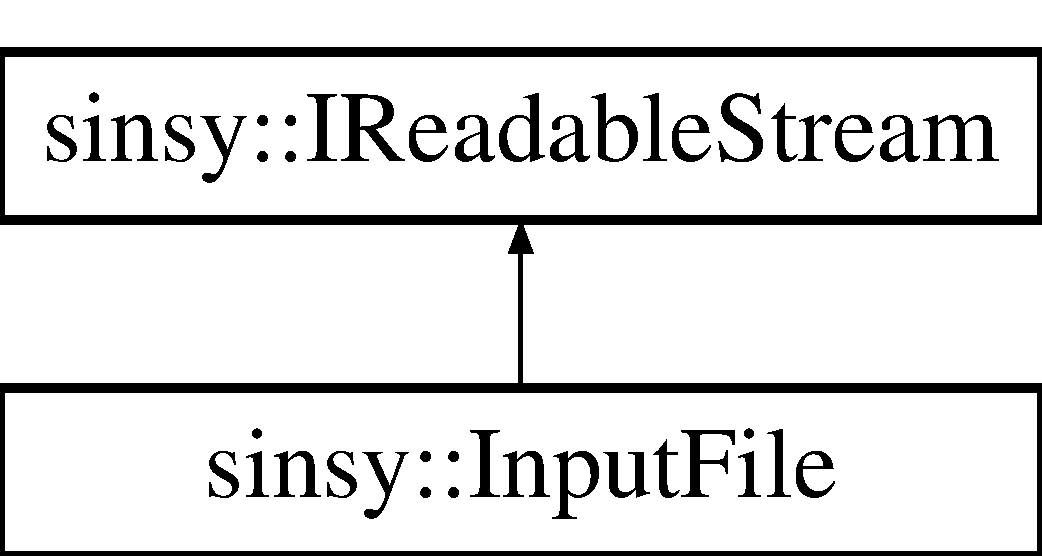
\includegraphics[height=2.000000cm]{classsinsy_1_1InputFile}
\end{center}
\end{figure}
\subsection*{\-Public \-Member \-Functions}
\begin{DoxyCompactItemize}
\item 
\hypertarget{classsinsy_1_1InputFile_a639375676099652952b522f0e3fd3a0d}{\hyperlink{classsinsy_1_1InputFile_a639375676099652952b522f0e3fd3a0d}{\-Input\-File} ()}\label{classsinsy_1_1InputFile_a639375676099652952b522f0e3fd3a0d}

\begin{DoxyCompactList}\small\item\em constructor \end{DoxyCompactList}\item 
\hypertarget{classsinsy_1_1InputFile_a5475344d19ebba6cae31a8695ac402a5}{\hyperlink{classsinsy_1_1InputFile_a5475344d19ebba6cae31a8695ac402a5}{\-Input\-File} (const std\-::string \&fpath)}\label{classsinsy_1_1InputFile_a5475344d19ebba6cae31a8695ac402a5}

\begin{DoxyCompactList}\small\item\em constructor \end{DoxyCompactList}\item 
\hypertarget{classsinsy_1_1InputFile_a184a592debf38e724f5c709e0b8b4eac}{virtual \hyperlink{classsinsy_1_1InputFile_a184a592debf38e724f5c709e0b8b4eac}{$\sim$\-Input\-File} ()}\label{classsinsy_1_1InputFile_a184a592debf38e724f5c709e0b8b4eac}

\begin{DoxyCompactList}\small\item\em destructor \end{DoxyCompactList}\item 
size\-\_\-t \hyperlink{classsinsy_1_1InputFile_a034391207b94b6b99d8c4a0c0d6f2f44}{read} (void $\ast$buffer, size\-\_\-t size)  throw (\-Stream\-Exception)
\begin{DoxyCompactList}\small\item\em read from stream \end{DoxyCompactList}\item 
\hypertarget{classsinsy_1_1InputFile_a64c7e6611d1bfd3f629e4318863345a3}{void \hyperlink{classsinsy_1_1InputFile_a64c7e6611d1bfd3f629e4318863345a3}{open} (const std\-::string \&fpath)}\label{classsinsy_1_1InputFile_a64c7e6611d1bfd3f629e4318863345a3}

\begin{DoxyCompactList}\small\item\em open \end{DoxyCompactList}\item 
\hypertarget{classsinsy_1_1InputFile_a5d1491bcfa54c25433617b42f1bba866}{void \hyperlink{classsinsy_1_1InputFile_a5d1491bcfa54c25433617b42f1bba866}{close} ()}\label{classsinsy_1_1InputFile_a5d1491bcfa54c25433617b42f1bba866}

\begin{DoxyCompactList}\small\item\em close \end{DoxyCompactList}\item 
\hypertarget{classsinsy_1_1InputFile_a33db202bf4cae0418e6ceff569c76429}{bool \hyperlink{classsinsy_1_1InputFile_a33db202bf4cae0418e6ceff569c76429}{is\-Valid} () const }\label{classsinsy_1_1InputFile_a33db202bf4cae0418e6ceff569c76429}

\begin{DoxyCompactList}\small\item\em stream is valid or not \end{DoxyCompactList}\end{DoxyCompactItemize}


\subsection{\-Member \-Function \-Documentation}
\hypertarget{classsinsy_1_1InputFile_a034391207b94b6b99d8c4a0c0d6f2f44}{\index{sinsy\-::\-Input\-File@{sinsy\-::\-Input\-File}!read@{read}}
\index{read@{read}!sinsy::InputFile@{sinsy\-::\-Input\-File}}
\subsubsection[{read}]{\setlength{\rightskip}{0pt plus 5cm}size\-\_\-t {\bf \-Input\-File\-::read} (
\begin{DoxyParamCaption}
\item[{void $\ast$}]{buffer, }
\item[{size\-\_\-t}]{size}
\end{DoxyParamCaption}
)  throw ({\bf \-Stream\-Exception})\hspace{0.3cm}{\ttfamily  \mbox{[}virtual\mbox{]}}}}\label{classsinsy_1_1InputFile_a034391207b94b6b99d8c4a0c0d6f2f44}


read from stream 

read data from stream


\begin{DoxyParams}{\-Parameters}
{\em buffer} & buffer for read data \\
\hline
{\em byte} & byte you want to read \\
\hline
\end{DoxyParams}
\begin{DoxyReturn}{\-Returns}
read bytes (0 \-: end of stream) 
\end{DoxyReturn}


\-Implements \hyperlink{classsinsy_1_1IReadableStream_acdbc2655936e8b8bbda0148b2a9c6c59}{sinsy\-::\-I\-Readable\-Stream}.



\-The documentation for this class was generated from the following files\-:\begin{DoxyCompactItemize}
\item 
lib/util/\-Input\-File.\-h\item 
lib/util/\-Input\-File.\-cpp\end{DoxyCompactItemize}

\hypertarget{classsinsy_1_1IPhonemeLabel}{\section{sinsy\-:\-:\-I\-Phoneme\-Label \-Class \-Reference}
\label{classsinsy_1_1IPhonemeLabel}\index{sinsy\-::\-I\-Phoneme\-Label@{sinsy\-::\-I\-Phoneme\-Label}}
}
\subsection*{\-Public \-Member \-Functions}
\begin{DoxyCompactItemize}
\item 
\hypertarget{classsinsy_1_1IPhonemeLabel_a5f7b131285ecf6d9041617cc5c126814}{virtual \hyperlink{classsinsy_1_1IPhonemeLabel_a5f7b131285ecf6d9041617cc5c126814}{$\sim$\-I\-Phoneme\-Label} ()}\label{classsinsy_1_1IPhonemeLabel_a5f7b131285ecf6d9041617cc5c126814}

\begin{DoxyCompactList}\small\item\em destructor \end{DoxyCompactList}\item 
\hypertarget{classsinsy_1_1IPhonemeLabel_a83ec4ed831f7d685bbd13c136d4bee85}{virtual void \hyperlink{classsinsy_1_1IPhonemeLabel_a83ec4ed831f7d685bbd13c136d4bee85}{set\-Type} (const std\-::string \&value)=0}\label{classsinsy_1_1IPhonemeLabel_a83ec4ed831f7d685bbd13c136d4bee85}

\begin{DoxyCompactList}\small\item\em set type \end{DoxyCompactList}\item 
\hypertarget{classsinsy_1_1IPhonemeLabel_a5b39af1d297171b914c5f0c8114c28d4}{virtual void \hyperlink{classsinsy_1_1IPhonemeLabel_a5b39af1d297171b914c5f0c8114c28d4}{set\-Name} (const std\-::string \&name)=0}\label{classsinsy_1_1IPhonemeLabel_a5b39af1d297171b914c5f0c8114c28d4}

\begin{DoxyCompactList}\small\item\em set name \end{DoxyCompactList}\item 
\hypertarget{classsinsy_1_1IPhonemeLabel_a7de966d57f1fd1f16af79382f05c2d42}{virtual void \hyperlink{classsinsy_1_1IPhonemeLabel_a7de966d57f1fd1f16af79382f05c2d42}{set\-Flag} (size\-\_\-t flag)=0}\label{classsinsy_1_1IPhonemeLabel_a7de966d57f1fd1f16af79382f05c2d42}

\begin{DoxyCompactList}\small\item\em set flag \end{DoxyCompactList}\item 
\hypertarget{classsinsy_1_1IPhonemeLabel_a37f8e6ee77544d4e1b29c3161a3da1aa}{virtual void \hyperlink{classsinsy_1_1IPhonemeLabel_a37f8e6ee77544d4e1b29c3161a3da1aa}{set\-Position\-In\-Syllable} (size\-\_\-t idx, size\-\_\-t max)=0}\label{classsinsy_1_1IPhonemeLabel_a37f8e6ee77544d4e1b29c3161a3da1aa}

\begin{DoxyCompactList}\small\item\em set position in syllable \end{DoxyCompactList}\end{DoxyCompactItemize}


\-The documentation for this class was generated from the following file\-:\begin{DoxyCompactItemize}
\item 
lib/label/\-I\-Phoneme\-Label.\-h\end{DoxyCompactItemize}

\hypertarget{classsinsy_1_1IReadableStream}{\section{sinsy\-:\-:\-I\-Readable\-Stream \-Class \-Reference}
\label{classsinsy_1_1IReadableStream}\index{sinsy\-::\-I\-Readable\-Stream@{sinsy\-::\-I\-Readable\-Stream}}
}
\-Inheritance diagram for sinsy\-:\-:\-I\-Readable\-Stream\-:\begin{figure}[H]
\begin{center}
\leavevmode
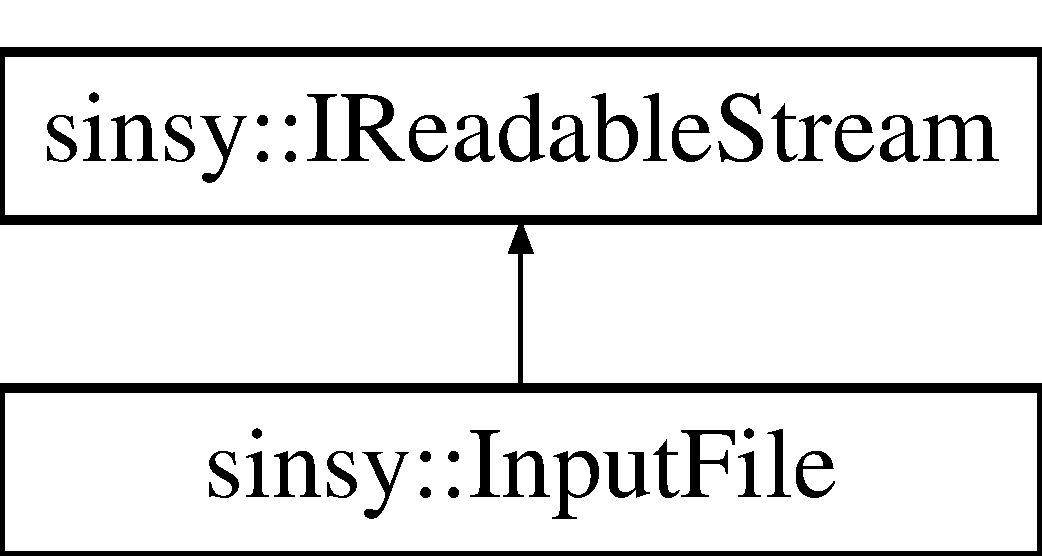
\includegraphics[height=2.000000cm]{classsinsy_1_1IReadableStream}
\end{center}
\end{figure}
\subsection*{\-Public \-Member \-Functions}
\begin{DoxyCompactItemize}
\item 
\hypertarget{classsinsy_1_1IReadableStream_a07d70bcc08019730c2f2e68ac3f41b08}{virtual \hyperlink{classsinsy_1_1IReadableStream_a07d70bcc08019730c2f2e68ac3f41b08}{$\sim$\-I\-Readable\-Stream} ()}\label{classsinsy_1_1IReadableStream_a07d70bcc08019730c2f2e68ac3f41b08}

\begin{DoxyCompactList}\small\item\em destructor \end{DoxyCompactList}\item 
virtual size\-\_\-t \hyperlink{classsinsy_1_1IReadableStream_acdbc2655936e8b8bbda0148b2a9c6c59}{read} (void $\ast$buffer, size\-\_\-t byte)=0  throw (\-Stream\-Exception)
\end{DoxyCompactItemize}


\subsection{\-Member \-Function \-Documentation}
\hypertarget{classsinsy_1_1IReadableStream_acdbc2655936e8b8bbda0148b2a9c6c59}{\index{sinsy\-::\-I\-Readable\-Stream@{sinsy\-::\-I\-Readable\-Stream}!read@{read}}
\index{read@{read}!sinsy::IReadableStream@{sinsy\-::\-I\-Readable\-Stream}}
\subsubsection[{read}]{\setlength{\rightskip}{0pt plus 5cm}virtual size\-\_\-t {\bf sinsy\-::\-I\-Readable\-Stream\-::read} (
\begin{DoxyParamCaption}
\item[{void $\ast$}]{buffer, }
\item[{size\-\_\-t}]{byte}
\end{DoxyParamCaption}
)  throw ({\bf \-Stream\-Exception})\hspace{0.3cm}{\ttfamily  \mbox{[}pure virtual\mbox{]}}}}\label{classsinsy_1_1IReadableStream_acdbc2655936e8b8bbda0148b2a9c6c59}
read data from stream


\begin{DoxyParams}{\-Parameters}
{\em buffer} & buffer for read data \\
\hline
{\em byte} & byte you want to read \\
\hline
\end{DoxyParams}
\begin{DoxyReturn}{\-Returns}
read bytes (0 \-: end of stream) 
\end{DoxyReturn}


\-Implemented in \hyperlink{classsinsy_1_1InputFile_a034391207b94b6b99d8c4a0c0d6f2f44}{sinsy\-::\-Input\-File}.



\-The documentation for this class was generated from the following file\-:\begin{DoxyCompactItemize}
\item 
lib/util/\-I\-Readable\-Stream.\-h\end{DoxyCompactItemize}

\hypertarget{classsinsy_1_1IScoreWritable}{\section{sinsy\-:\-:\-I\-Score\-Writable \-Class \-Reference}
\label{classsinsy_1_1IScoreWritable}\index{sinsy\-::\-I\-Score\-Writable@{sinsy\-::\-I\-Score\-Writable}}
}
\-Inheritance diagram for sinsy\-:\-:\-I\-Score\-Writable\-:\begin{figure}[H]
\begin{center}
\leavevmode
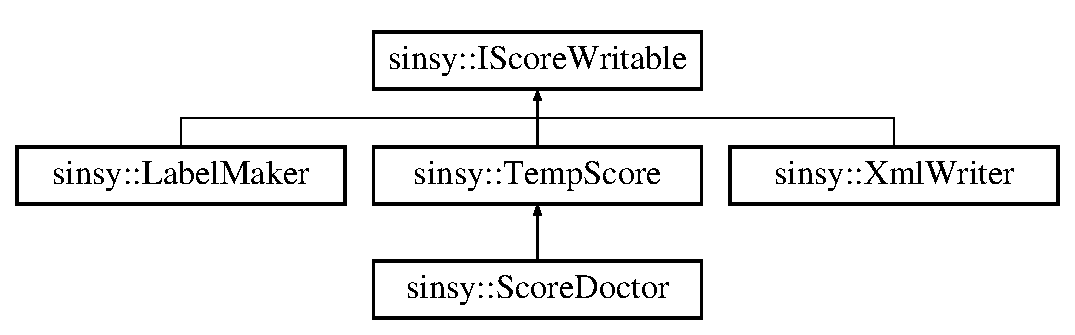
\includegraphics[height=3.000000cm]{classsinsy_1_1IScoreWritable}
\end{center}
\end{figure}
\subsection*{\-Public \-Member \-Functions}
\begin{DoxyCompactItemize}
\item 
\hypertarget{classsinsy_1_1IScoreWritable_ad174b82ab93af6abd98ed224600f7b63}{virtual \hyperlink{classsinsy_1_1IScoreWritable_ad174b82ab93af6abd98ed224600f7b63}{$\sim$\-I\-Score\-Writable} ()}\label{classsinsy_1_1IScoreWritable_ad174b82ab93af6abd98ed224600f7b63}

\begin{DoxyCompactList}\small\item\em destructor \end{DoxyCompactList}\item 
\hypertarget{classsinsy_1_1IScoreWritable_ae891ee3c7cf1e2243d9d042b4c277b92}{virtual void {\bfseries set\-Encoding} (const std\-::string \&encoding)=0}\label{classsinsy_1_1IScoreWritable_ae891ee3c7cf1e2243d9d042b4c277b92}

\item 
\hypertarget{classsinsy_1_1IScoreWritable_ac7d05ec388c44450f2b036b691ff652e}{virtual void \hyperlink{classsinsy_1_1IScoreWritable_ac7d05ec388c44450f2b036b691ff652e}{change\-Tempo} (double tempo)=0}\label{classsinsy_1_1IScoreWritable_ac7d05ec388c44450f2b036b691ff652e}

\begin{DoxyCompactList}\small\item\em change tempo \end{DoxyCompactList}\item 
\hypertarget{classsinsy_1_1IScoreWritable_a8a953ab53edb884601eb19c65dee81e7}{virtual void \hyperlink{classsinsy_1_1IScoreWritable_a8a953ab53edb884601eb19c65dee81e7}{change\-Beat} (const \hyperlink{classsinsy_1_1Beat}{\-Beat} \&beat)=0}\label{classsinsy_1_1IScoreWritable_a8a953ab53edb884601eb19c65dee81e7}

\begin{DoxyCompactList}\small\item\em change beat \end{DoxyCompactList}\item 
\hypertarget{classsinsy_1_1IScoreWritable_a20a40fe2d8418648208d8e4b2dd1a31d}{virtual void \hyperlink{classsinsy_1_1IScoreWritable_a20a40fe2d8418648208d8e4b2dd1a31d}{change\-Dynamics} (const \hyperlink{classsinsy_1_1Dynamics}{\-Dynamics} \&dynamics)=0}\label{classsinsy_1_1IScoreWritable_a20a40fe2d8418648208d8e4b2dd1a31d}

\begin{DoxyCompactList}\small\item\em change dynamics \end{DoxyCompactList}\item 
\hypertarget{classsinsy_1_1IScoreWritable_aab1dfca13aebe9dbb2ed5a82d991ae71}{virtual void \hyperlink{classsinsy_1_1IScoreWritable_aab1dfca13aebe9dbb2ed5a82d991ae71}{change\-Key} (const \hyperlink{classsinsy_1_1Key}{\-Key} \&key)=0}\label{classsinsy_1_1IScoreWritable_aab1dfca13aebe9dbb2ed5a82d991ae71}

\begin{DoxyCompactList}\small\item\em change key \end{DoxyCompactList}\item 
\hypertarget{classsinsy_1_1IScoreWritable_afe63162fab1fc648b1401ea83791a840}{virtual void \hyperlink{classsinsy_1_1IScoreWritable_afe63162fab1fc648b1401ea83791a840}{start\-Crescendo} ()=0}\label{classsinsy_1_1IScoreWritable_afe63162fab1fc648b1401ea83791a840}

\begin{DoxyCompactList}\small\item\em start crescendo \end{DoxyCompactList}\item 
\hypertarget{classsinsy_1_1IScoreWritable_a32d8c5fd5e3bee214fb7fad3b72fc4de}{virtual void \hyperlink{classsinsy_1_1IScoreWritable_a32d8c5fd5e3bee214fb7fad3b72fc4de}{start\-Diminuendo} ()=0}\label{classsinsy_1_1IScoreWritable_a32d8c5fd5e3bee214fb7fad3b72fc4de}

\begin{DoxyCompactList}\small\item\em start diminuendo \end{DoxyCompactList}\item 
\hypertarget{classsinsy_1_1IScoreWritable_a5869fa4b213eb9208284a3b768c6f753}{virtual void \hyperlink{classsinsy_1_1IScoreWritable_a5869fa4b213eb9208284a3b768c6f753}{stop\-Crescendo} ()=0}\label{classsinsy_1_1IScoreWritable_a5869fa4b213eb9208284a3b768c6f753}

\begin{DoxyCompactList}\small\item\em stop crescendo \end{DoxyCompactList}\item 
\hypertarget{classsinsy_1_1IScoreWritable_a8557cc67898a47a73d884a8b7eb2ebf2}{virtual void \hyperlink{classsinsy_1_1IScoreWritable_a8557cc67898a47a73d884a8b7eb2ebf2}{stop\-Diminuendo} ()=0}\label{classsinsy_1_1IScoreWritable_a8557cc67898a47a73d884a8b7eb2ebf2}

\begin{DoxyCompactList}\small\item\em stop diminuendo \end{DoxyCompactList}\item 
\hypertarget{classsinsy_1_1IScoreWritable_a00cee3ee0ba767b1bda8a8a7e2ad63aa}{virtual void \hyperlink{classsinsy_1_1IScoreWritable_a00cee3ee0ba767b1bda8a8a7e2ad63aa}{add\-Note} (const \hyperlink{classsinsy_1_1Note}{\-Note} \&note)=0}\label{classsinsy_1_1IScoreWritable_a00cee3ee0ba767b1bda8a8a7e2ad63aa}

\begin{DoxyCompactList}\small\item\em add note \end{DoxyCompactList}\end{DoxyCompactItemize}


\-The documentation for this class was generated from the following file\-:\begin{DoxyCompactItemize}
\item 
lib/score/\-I\-Score\-Writable.\-h\end{DoxyCompactItemize}

\hypertarget{classsinsy_1_1IScoreWriter}{\section{sinsy\-:\-:\-I\-Score\-Writer \-Class \-Reference}
\label{classsinsy_1_1IScoreWriter}\index{sinsy\-::\-I\-Score\-Writer@{sinsy\-::\-I\-Score\-Writer}}
}
\-Inheritance diagram for sinsy\-:\-:\-I\-Score\-Writer\-:\begin{figure}[H]
\begin{center}
\leavevmode
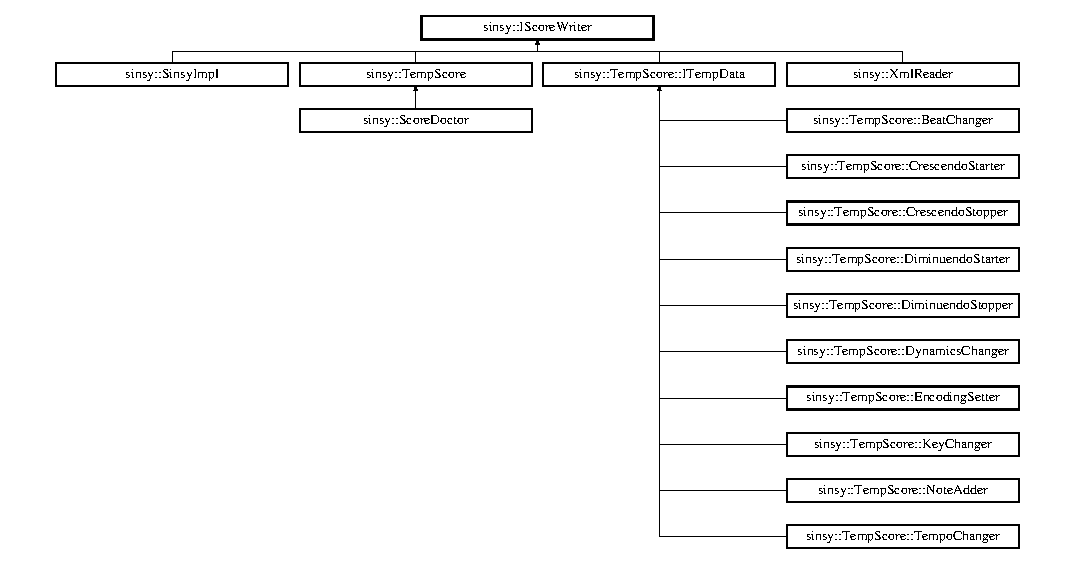
\includegraphics[height=7.148936cm]{classsinsy_1_1IScoreWriter}
\end{center}
\end{figure}
\subsection*{\-Public \-Member \-Functions}
\begin{DoxyCompactItemize}
\item 
\hypertarget{classsinsy_1_1IScoreWriter_aca80577a76a852831ec4a95ae03117d0}{virtual \hyperlink{classsinsy_1_1IScoreWriter_aca80577a76a852831ec4a95ae03117d0}{$\sim$\-I\-Score\-Writer} ()}\label{classsinsy_1_1IScoreWriter_aca80577a76a852831ec4a95ae03117d0}

\begin{DoxyCompactList}\small\item\em destructor \end{DoxyCompactList}\item 
\hypertarget{classsinsy_1_1IScoreWriter_a15b81f3e78834610052da3cc48e0f7ad}{virtual void \hyperlink{classsinsy_1_1IScoreWriter_a15b81f3e78834610052da3cc48e0f7ad}{write} (\hyperlink{classsinsy_1_1IScoreWritable}{\-I\-Score\-Writable} \&writable) const =0}\label{classsinsy_1_1IScoreWriter_a15b81f3e78834610052da3cc48e0f7ad}

\begin{DoxyCompactList}\small\item\em write score \end{DoxyCompactList}\end{DoxyCompactItemize}


\-The documentation for this class was generated from the following file\-:\begin{DoxyCompactItemize}
\item 
lib/score/\-I\-Score\-Writer.\-h\end{DoxyCompactItemize}

\hypertarget{classsinsy_1_1IStringWritable}{\section{sinsy\-:\-:\-I\-String\-Writable \-Class \-Reference}
\label{classsinsy_1_1IStringWritable}\index{sinsy\-::\-I\-String\-Writable@{sinsy\-::\-I\-String\-Writable}}
}
\-Inheritance diagram for sinsy\-:\-:\-I\-String\-Writable\-:\begin{figure}[H]
\begin{center}
\leavevmode
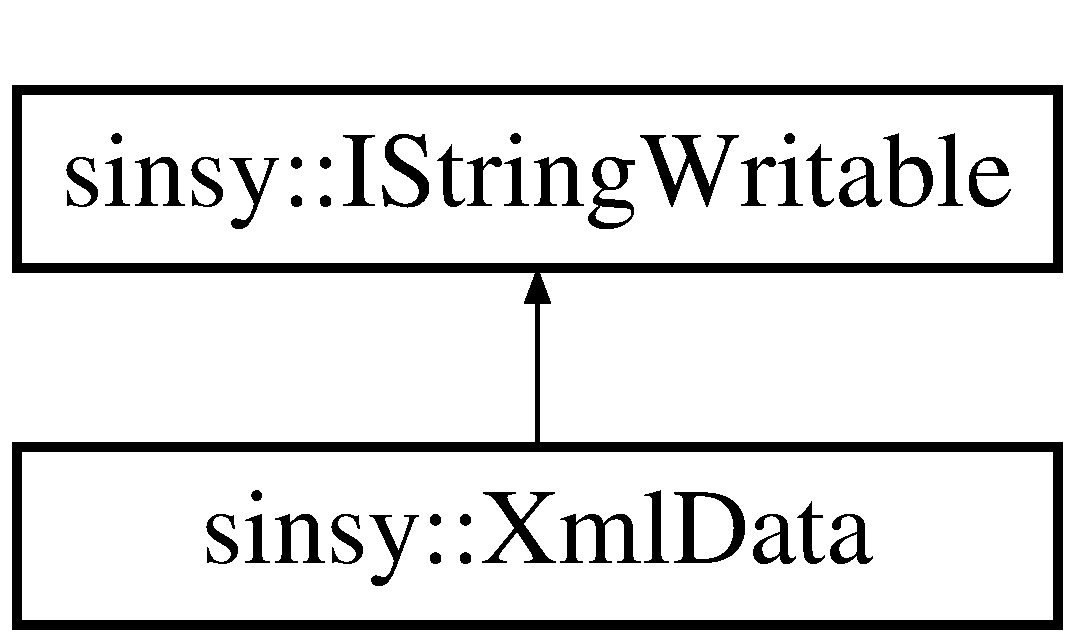
\includegraphics[height=2.000000cm]{classsinsy_1_1IStringWritable}
\end{center}
\end{figure}
\subsection*{\-Public \-Member \-Functions}
\begin{DoxyCompactItemize}
\item 
\hypertarget{classsinsy_1_1IStringWritable_a4c6d1dbf3c60947b427be8e0cae937da}{virtual \hyperlink{classsinsy_1_1IStringWritable_a4c6d1dbf3c60947b427be8e0cae937da}{$\sim$\-I\-String\-Writable} ()}\label{classsinsy_1_1IStringWritable_a4c6d1dbf3c60947b427be8e0cae937da}

\begin{DoxyCompactList}\small\item\em destructor \end{DoxyCompactList}\item 
\hypertarget{classsinsy_1_1IStringWritable_a044c5bb33002dacec9bbdbf2dc0fbe23}{virtual std\-::ostream \& \hyperlink{classsinsy_1_1IStringWritable_a044c5bb33002dacec9bbdbf2dc0fbe23}{to\-String\-Stream} (std\-::ostream \&) const =0}\label{classsinsy_1_1IStringWritable_a044c5bb33002dacec9bbdbf2dc0fbe23}

\begin{DoxyCompactList}\small\item\em to string stream \end{DoxyCompactList}\end{DoxyCompactItemize}


\-The documentation for this class was generated from the following file\-:\begin{DoxyCompactItemize}
\item 
lib/util/\-I\-Stringable.\-h\end{DoxyCompactItemize}

\hypertarget{classsinsy_1_1ISyllableLabel}{\section{sinsy\-:\-:\-I\-Syllable\-Label \-Class \-Reference}
\label{classsinsy_1_1ISyllableLabel}\index{sinsy\-::\-I\-Syllable\-Label@{sinsy\-::\-I\-Syllable\-Label}}
}
\subsection*{\-Public \-Member \-Functions}
\begin{DoxyCompactItemize}
\item 
\hypertarget{classsinsy_1_1ISyllableLabel_a8676d776bfc6d5938044083271ad005b}{virtual \hyperlink{classsinsy_1_1ISyllableLabel_a8676d776bfc6d5938044083271ad005b}{$\sim$\-I\-Syllable\-Label} ()}\label{classsinsy_1_1ISyllableLabel_a8676d776bfc6d5938044083271ad005b}

\begin{DoxyCompactList}\small\item\em destructor \end{DoxyCompactList}\item 
\hypertarget{classsinsy_1_1ISyllableLabel_acc166ab50fd7af6f4e5c23e08e46f2f1}{virtual void \hyperlink{classsinsy_1_1ISyllableLabel_acc166ab50fd7af6f4e5c23e08e46f2f1}{set\-Phoneme\-Num} (size\-\_\-t num)=0}\label{classsinsy_1_1ISyllableLabel_acc166ab50fd7af6f4e5c23e08e46f2f1}

\begin{DoxyCompactList}\small\item\em set number of phonemes \end{DoxyCompactList}\item 
\hypertarget{classsinsy_1_1ISyllableLabel_ae36d20bc3c756c3a6fb26b7c378ac754}{virtual void \hyperlink{classsinsy_1_1ISyllableLabel_ae36d20bc3c756c3a6fb26b7c378ac754}{set\-Position\-In\-Note} (size\-\_\-t idx, size\-\_\-t max)=0}\label{classsinsy_1_1ISyllableLabel_ae36d20bc3c756c3a6fb26b7c378ac754}

\begin{DoxyCompactList}\small\item\em set position in note \end{DoxyCompactList}\item 
\hypertarget{classsinsy_1_1ISyllableLabel_a4452a2097df590bd00c428fbbb0a5d34}{virtual void \hyperlink{classsinsy_1_1ISyllableLabel_a4452a2097df590bd00c428fbbb0a5d34}{set\-Language} (const std\-::string \&language)=0}\label{classsinsy_1_1ISyllableLabel_a4452a2097df590bd00c428fbbb0a5d34}

\begin{DoxyCompactList}\small\item\em set language \end{DoxyCompactList}\item 
\hypertarget{classsinsy_1_1ISyllableLabel_aa6dee3cda59e6b20373c92341fd1b361}{virtual void \hyperlink{classsinsy_1_1ISyllableLabel_aa6dee3cda59e6b20373c92341fd1b361}{set\-Lang\-Dependent\-Info} (const std\-::string \&info)=0}\label{classsinsy_1_1ISyllableLabel_aa6dee3cda59e6b20373c92341fd1b361}

\begin{DoxyCompactList}\small\item\em set language-\/dependent infomation \end{DoxyCompactList}\end{DoxyCompactItemize}


\-The documentation for this class was generated from the following file\-:\begin{DoxyCompactItemize}
\item 
lib/label/\-I\-Syllable\-Label.\-h\end{DoxyCompactItemize}

\hypertarget{classsinsy_1_1TempScore_1_1ITempData}{\section{sinsy\-:\-:\-Temp\-Score\-:\-:\-I\-Temp\-Data \-Class \-Reference}
\label{classsinsy_1_1TempScore_1_1ITempData}\index{sinsy\-::\-Temp\-Score\-::\-I\-Temp\-Data@{sinsy\-::\-Temp\-Score\-::\-I\-Temp\-Data}}
}
\-Inheritance diagram for sinsy\-:\-:\-Temp\-Score\-:\-:\-I\-Temp\-Data\-:\begin{figure}[H]
\begin{center}
\leavevmode
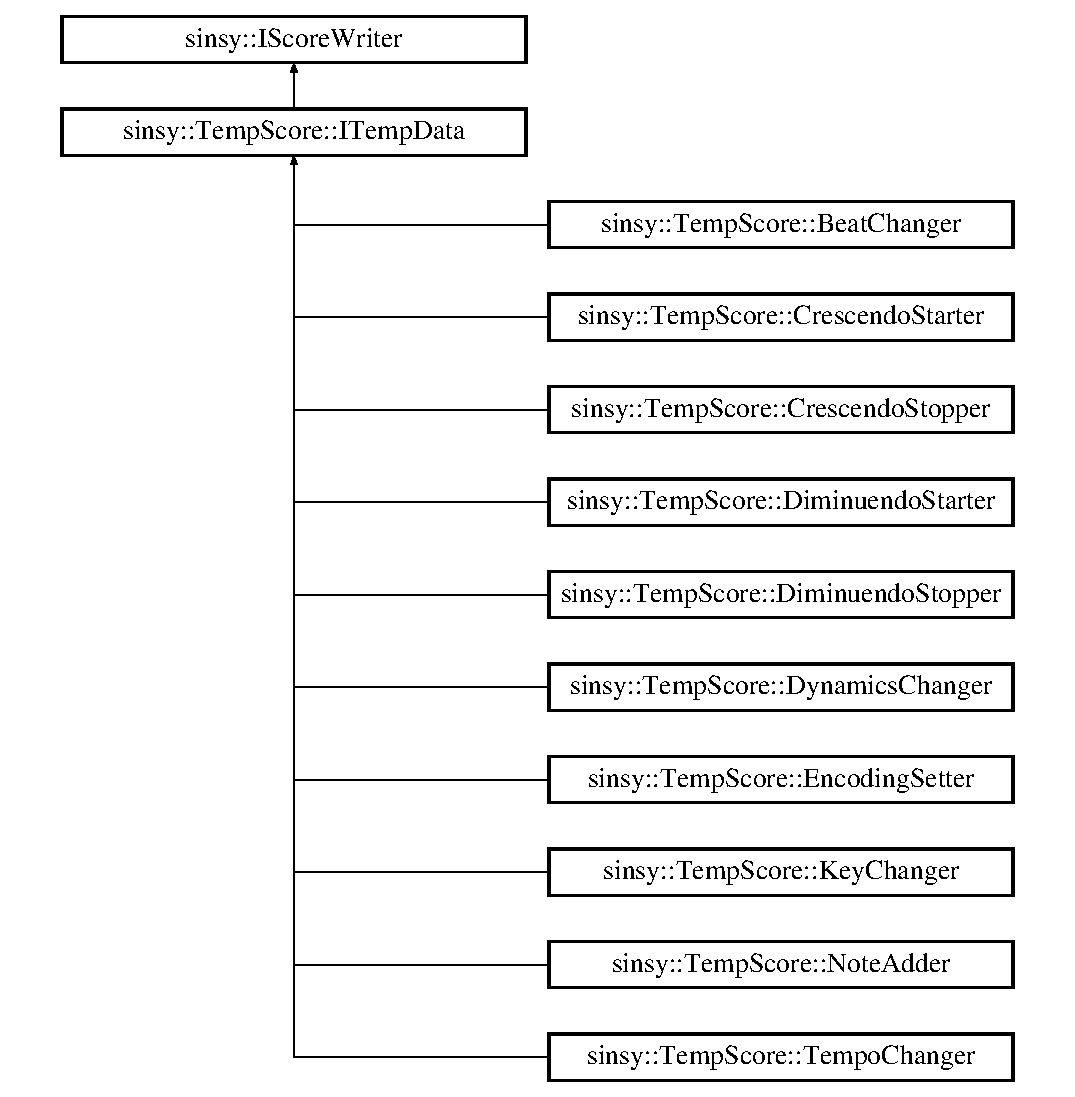
\includegraphics[height=12.000000cm]{classsinsy_1_1TempScore_1_1ITempData}
\end{center}
\end{figure}
\subsection*{\-Public \-Member \-Functions}
\begin{DoxyCompactItemize}
\item 
\hypertarget{classsinsy_1_1TempScore_1_1ITempData_a84c9771b226d16b5a47b76d7ef0c01d4}{virtual \hyperlink{classsinsy_1_1TempScore_1_1ITempData_a84c9771b226d16b5a47b76d7ef0c01d4}{$\sim$\-I\-Temp\-Data} ()}\label{classsinsy_1_1TempScore_1_1ITempData_a84c9771b226d16b5a47b76d7ef0c01d4}

\begin{DoxyCompactList}\small\item\em destructor \end{DoxyCompactList}\item 
\hypertarget{classsinsy_1_1TempScore_1_1ITempData_ab6d83a865088b42b62dc5a0a82e47fa5}{virtual void \hyperlink{classsinsy_1_1TempScore_1_1ITempData_ab6d83a865088b42b62dc5a0a82e47fa5}{write} (\hyperlink{classsinsy_1_1IScoreWritable}{\-I\-Score\-Writable} \&) const =0}\label{classsinsy_1_1TempScore_1_1ITempData_ab6d83a865088b42b62dc5a0a82e47fa5}

\begin{DoxyCompactList}\small\item\em write \end{DoxyCompactList}\end{DoxyCompactItemize}


\-The documentation for this class was generated from the following file\-:\begin{DoxyCompactItemize}
\item 
lib/temporary/\-Temp\-Score.\-h\end{DoxyCompactItemize}

\hypertarget{classsinsy_1_1IWritableStream}{\section{sinsy\-:\-:\-I\-Writable\-Stream \-Class \-Reference}
\label{classsinsy_1_1IWritableStream}\index{sinsy\-::\-I\-Writable\-Stream@{sinsy\-::\-I\-Writable\-Stream}}
}
\-Inheritance diagram for sinsy\-:\-:\-I\-Writable\-Stream\-:\begin{figure}[H]
\begin{center}
\leavevmode
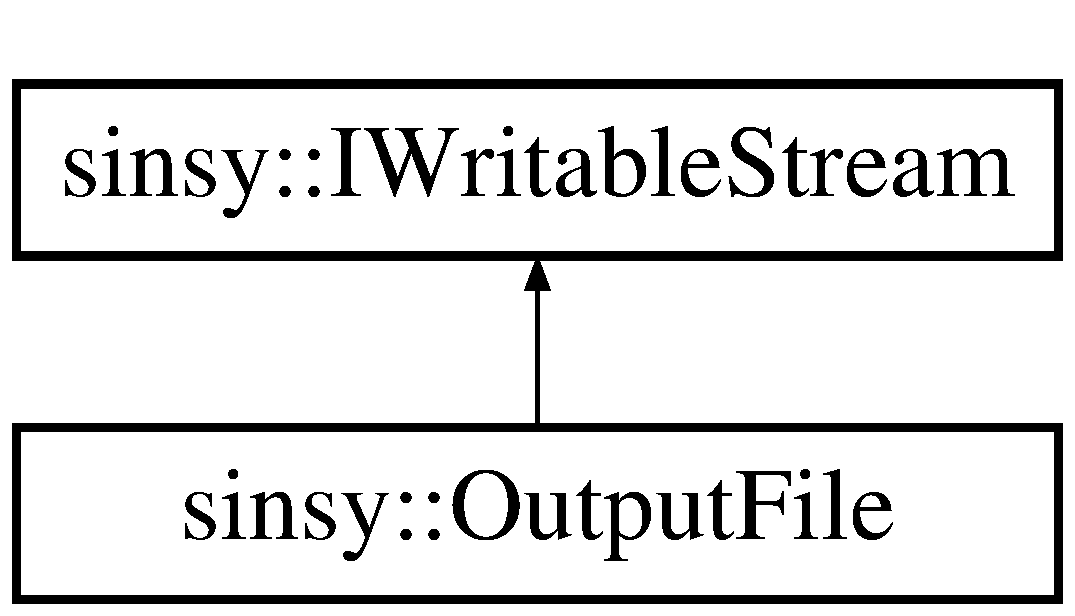
\includegraphics[height=2.000000cm]{classsinsy_1_1IWritableStream}
\end{center}
\end{figure}
\subsection*{\-Public \-Member \-Functions}
\begin{DoxyCompactItemize}
\item 
\hypertarget{classsinsy_1_1IWritableStream_a7daec491e272ee964d13a567e6adb2f3}{virtual \hyperlink{classsinsy_1_1IWritableStream_a7daec491e272ee964d13a567e6adb2f3}{$\sim$\-I\-Writable\-Stream} ()}\label{classsinsy_1_1IWritableStream_a7daec491e272ee964d13a567e6adb2f3}

\begin{DoxyCompactList}\small\item\em destructor \end{DoxyCompactList}\item 
virtual size\-\_\-t \hyperlink{classsinsy_1_1IWritableStream_a0e7f8f7e1c41c6edd1b0d540957ba1cc}{write} (const void $\ast$buffer, size\-\_\-t byte)=0  throw (\-Stream\-Exception)
\end{DoxyCompactItemize}


\subsection{\-Member \-Function \-Documentation}
\hypertarget{classsinsy_1_1IWritableStream_a0e7f8f7e1c41c6edd1b0d540957ba1cc}{\index{sinsy\-::\-I\-Writable\-Stream@{sinsy\-::\-I\-Writable\-Stream}!write@{write}}
\index{write@{write}!sinsy::IWritableStream@{sinsy\-::\-I\-Writable\-Stream}}
\subsubsection[{write}]{\setlength{\rightskip}{0pt plus 5cm}virtual size\-\_\-t {\bf sinsy\-::\-I\-Writable\-Stream\-::write} (
\begin{DoxyParamCaption}
\item[{const void $\ast$}]{buffer, }
\item[{size\-\_\-t}]{byte}
\end{DoxyParamCaption}
)  throw ({\bf \-Stream\-Exception})\hspace{0.3cm}{\ttfamily  \mbox{[}pure virtual\mbox{]}}}}\label{classsinsy_1_1IWritableStream_a0e7f8f7e1c41c6edd1b0d540957ba1cc}
write data to stream 
\begin{DoxyParams}{\-Parameters}
{\em buffer} & buffer for data that you want to write \\
\hline
{\em byte} & byte you want to write \\
\hline
\end{DoxyParams}
\begin{DoxyReturn}{\-Returns}
write bytes 
\end{DoxyReturn}


\-Implemented in \hyperlink{classsinsy_1_1OutputFile_a50aa606271487a08ad2eb59268007f26}{sinsy\-::\-Output\-File}.



\-The documentation for this class was generated from the following file\-:\begin{DoxyCompactItemize}
\item 
lib/util/\-I\-Writable\-Stream.\-h\end{DoxyCompactItemize}

\hypertarget{classsinsy_1_1JConf}{\section{sinsy\-:\-:\-J\-Conf \-Class \-Reference}
\label{classsinsy_1_1JConf}\index{sinsy\-::\-J\-Conf@{sinsy\-::\-J\-Conf}}
}
\-Inheritance diagram for sinsy\-:\-:\-J\-Conf\-:\begin{figure}[H]
\begin{center}
\leavevmode
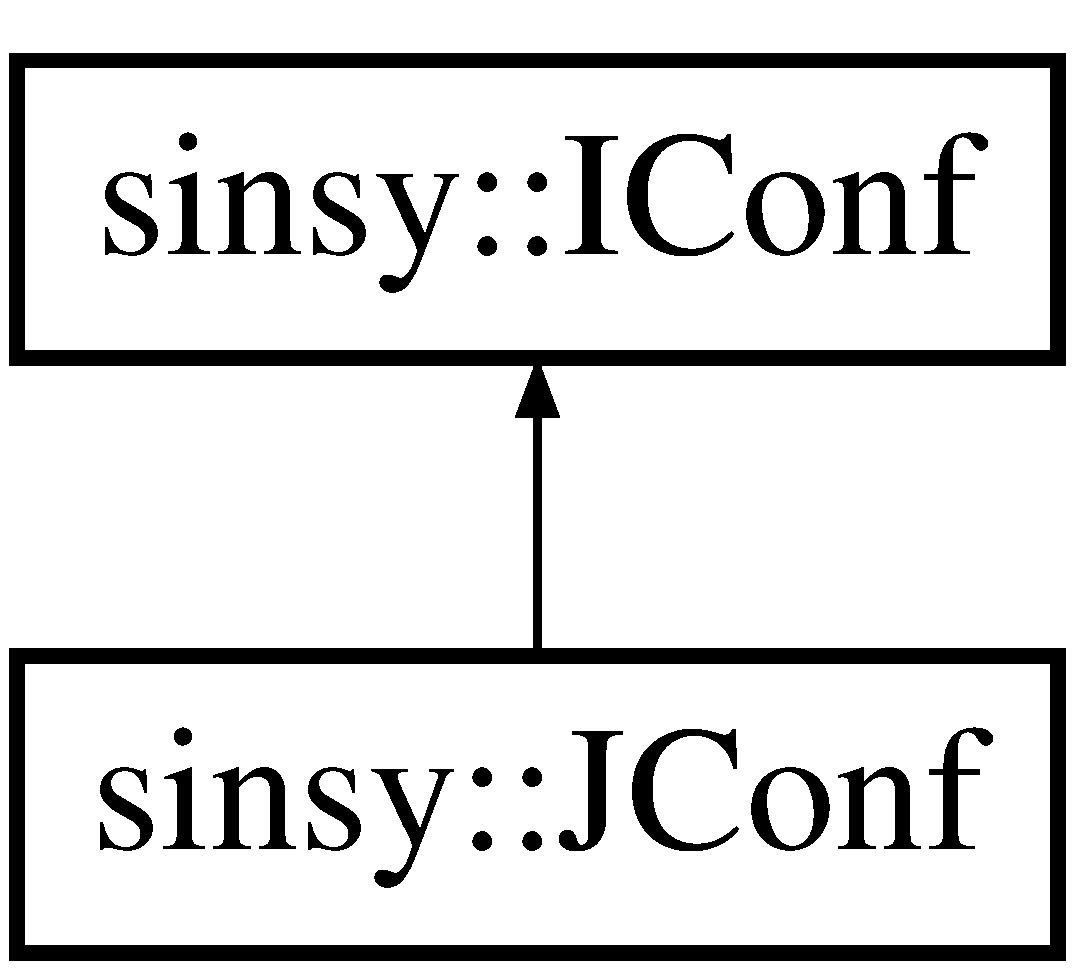
\includegraphics[height=2.000000cm]{classsinsy_1_1JConf}
\end{center}
\end{figure}
\subsection*{\-Public \-Member \-Functions}
\begin{DoxyCompactItemize}
\item 
\hyperlink{classsinsy_1_1JConf_a1bc3b834b00c92f78a42529252a89f95}{\-J\-Conf} (const std\-::string \&enc)
\begin{DoxyCompactList}\small\item\em constructor \end{DoxyCompactList}\item 
\hypertarget{classsinsy_1_1JConf_a6bbe7a54ed73b9bccb6abf6c8ca5ff2a}{virtual \hyperlink{classsinsy_1_1JConf_a6bbe7a54ed73b9bccb6abf6c8ca5ff2a}{$\sim$\-J\-Conf} ()}\label{classsinsy_1_1JConf_a6bbe7a54ed73b9bccb6abf6c8ca5ff2a}

\begin{DoxyCompactList}\small\item\em destructor \end{DoxyCompactList}\item 
bool \hyperlink{classsinsy_1_1JConf_a472b3cdcb61dace17ade9a5998d417a5}{read} (const std\-::string \&table, const std\-::string \&conf, const std\-::string \&macron)
\begin{DoxyCompactList}\small\item\em read phoneme table and config from files \end{DoxyCompactList}\item 
\hypertarget{classsinsy_1_1JConf_afb3b14617a4c8617b46a037e9237b47a}{virtual bool \hyperlink{classsinsy_1_1JConf_afb3b14617a4c8617b46a037e9237b47a}{convert} (const std\-::string \&enc, \-Convertable\-List\-::iterator begin, \-Convertable\-List\-::iterator end) const }\label{classsinsy_1_1JConf_afb3b14617a4c8617b46a037e9237b47a}

\begin{DoxyCompactList}\small\item\em convert lyrics to phonemes \end{DoxyCompactList}\item 
virtual std\-::string \hyperlink{classsinsy_1_1JConf_abab4dec7dd8ea8ef959b8c95df34ae07}{get\-Sil\-Str} () const 
\begin{DoxyCompactList}\small\item\em get sil str \end{DoxyCompactList}\item 
\hypertarget{classsinsy_1_1JConf_a7e92eca34eb52c61e8f687814df10fab}{bool \hyperlink{classsinsy_1_1JConf_a7e92eca34eb52c61e8f687814df10fab}{check\-Encoding} (const std\-::string \&enc) const }\label{classsinsy_1_1JConf_a7e92eca34eb52c61e8f687814df10fab}

\begin{DoxyCompactList}\small\item\em check encoding \end{DoxyCompactList}\item 
\hypertarget{classsinsy_1_1JConf_ae68ae803221f37058ba940f981f2b96f}{const \hyperlink{classsinsy_1_1MultibyteCharRange}{\-Multibyte\-Char\-Range} \& \hyperlink{classsinsy_1_1JConf_ae68ae803221f37058ba940f981f2b96f}{get\-Multibyte\-Char\-Range} () const }\label{classsinsy_1_1JConf_ae68ae803221f37058ba940f981f2b96f}

\begin{DoxyCompactList}\small\item\em get multibyte char range \end{DoxyCompactList}\end{DoxyCompactItemize}


\subsection{\-Constructor \& \-Destructor \-Documentation}
\hypertarget{classsinsy_1_1JConf_a1bc3b834b00c92f78a42529252a89f95}{\index{sinsy\-::\-J\-Conf@{sinsy\-::\-J\-Conf}!\-J\-Conf@{\-J\-Conf}}
\index{\-J\-Conf@{\-J\-Conf}!sinsy::JConf@{sinsy\-::\-J\-Conf}}
\subsubsection[{\-J\-Conf}]{\setlength{\rightskip}{0pt plus 5cm}{\bf \-J\-Conf\-::\-J\-Conf} (
\begin{DoxyParamCaption}
\item[{const std\-::string \&}]{enc}
\end{DoxyParamCaption}
)}}\label{classsinsy_1_1JConf_a1bc3b834b00c92f78a42529252a89f95}


constructor 

constructor


\begin{DoxyParams}{\-Parameters}
{\em enc} & encoding strings (e.\-g. \char`\"{}utf\-\_\-8, utf8, utf-\/8\char`\"{}) \\
\hline
\end{DoxyParams}


\subsection{\-Member \-Function \-Documentation}
\hypertarget{classsinsy_1_1JConf_abab4dec7dd8ea8ef959b8c95df34ae07}{\index{sinsy\-::\-J\-Conf@{sinsy\-::\-J\-Conf}!get\-Sil\-Str@{get\-Sil\-Str}}
\index{get\-Sil\-Str@{get\-Sil\-Str}!sinsy::JConf@{sinsy\-::\-J\-Conf}}
\subsubsection[{get\-Sil\-Str}]{\setlength{\rightskip}{0pt plus 5cm}std\-::string {\bf \-J\-Conf\-::get\-Sil\-Str} (
\begin{DoxyParamCaption}
{}
\end{DoxyParamCaption}
) const\hspace{0.3cm}{\ttfamily  \mbox{[}virtual\mbox{]}}}}\label{classsinsy_1_1JConf_abab4dec7dd8ea8ef959b8c95df34ae07}


get sil str 

get sil string

return sil str 

\-Implements \hyperlink{classsinsy_1_1IConf_a6b4b753e87291960ccc88867d97ef280}{sinsy\-::\-I\-Conf}.

\hypertarget{classsinsy_1_1JConf_a472b3cdcb61dace17ade9a5998d417a5}{\index{sinsy\-::\-J\-Conf@{sinsy\-::\-J\-Conf}!read@{read}}
\index{read@{read}!sinsy::JConf@{sinsy\-::\-J\-Conf}}
\subsubsection[{read}]{\setlength{\rightskip}{0pt plus 5cm}bool {\bf \-J\-Conf\-::read} (
\begin{DoxyParamCaption}
\item[{const std\-::string \&}]{table, }
\item[{const std\-::string \&}]{conf, }
\item[{const std\-::string \&}]{macron}
\end{DoxyParamCaption}
)}}\label{classsinsy_1_1JConf_a472b3cdcb61dace17ade9a5998d417a5}


read phoneme table and config from files 

read phoneme table and config from files


\begin{DoxyParams}{\-Parameters}
{\em table} & phoneme table file path \\
\hline
{\em conf} & config file path \\
\hline
\end{DoxyParams}
\begin{DoxyReturn}{\-Returns}
true if success 
\end{DoxyReturn}


\-The documentation for this class was generated from the following files\-:\begin{DoxyCompactItemize}
\item 
lib/japanese/\-J\-Conf.\-h\item 
lib/japanese/\-J\-Conf.\-cpp\end{DoxyCompactItemize}

\hypertarget{classsinsy_1_1Key}{\section{sinsy\-:\-:\-Key \-Class \-Reference}
\label{classsinsy_1_1Key}\index{sinsy\-::\-Key@{sinsy\-::\-Key}}
}
\subsection*{\-Public \-Member \-Functions}
\begin{DoxyCompactItemize}
\item 
\hypertarget{classsinsy_1_1Key_a22e51dbebb18c1d33ee8bba93a1b3b4d}{\hyperlink{classsinsy_1_1Key_a22e51dbebb18c1d33ee8bba93a1b3b4d}{\-Key} ()}\label{classsinsy_1_1Key_a22e51dbebb18c1d33ee8bba93a1b3b4d}

\begin{DoxyCompactList}\small\item\em constructor \end{DoxyCompactList}\item 
\hyperlink{classsinsy_1_1Key_a3065863c97c7805e454248655aaa0c92}{\-Key} (const \hyperlink{classsinsy_1_1Mode}{\-Mode} \&mode, int fifths)
\begin{DoxyCompactList}\small\item\em constructor \end{DoxyCompactList}\item 
\hypertarget{classsinsy_1_1Key_ae21c8e651ab4b4994f28cc339b809886}{\hyperlink{classsinsy_1_1Key_ae21c8e651ab4b4994f28cc339b809886}{\-Key} (const \hyperlink{classsinsy_1_1Key}{\-Key} \&obj)}\label{classsinsy_1_1Key_ae21c8e651ab4b4994f28cc339b809886}

\begin{DoxyCompactList}\small\item\em copy constructor \end{DoxyCompactList}\item 
\hypertarget{classsinsy_1_1Key_a92ff6ee5df282f6d7abb893fd14d81af}{virtual \hyperlink{classsinsy_1_1Key_a92ff6ee5df282f6d7abb893fd14d81af}{$\sim$\-Key} ()}\label{classsinsy_1_1Key_a92ff6ee5df282f6d7abb893fd14d81af}

\begin{DoxyCompactList}\small\item\em destructor \end{DoxyCompactList}\item 
\hypertarget{classsinsy_1_1Key_a2491a5000197f4b105a11c21b96c6afe}{\hyperlink{classsinsy_1_1Key}{\-Key} \& \hyperlink{classsinsy_1_1Key_a2491a5000197f4b105a11c21b96c6afe}{operator=} (const \hyperlink{classsinsy_1_1Key}{\-Key} \&obj)}\label{classsinsy_1_1Key_a2491a5000197f4b105a11c21b96c6afe}

\begin{DoxyCompactList}\small\item\em assignment operator \end{DoxyCompactList}\item 
bool \hyperlink{classsinsy_1_1Key_a742f3097f4ecbe1cb2a8e0b81b96f89e}{operator==} (const \hyperlink{classsinsy_1_1Key}{\-Key} \&obj) const 
\begin{DoxyCompactList}\small\item\em equal \end{DoxyCompactList}\item 
bool \hyperlink{classsinsy_1_1Key_a63958fac37a555816177428dd21493d9}{operator!=} (const \hyperlink{classsinsy_1_1Key}{\-Key} \&obj) const 
\begin{DoxyCompactList}\small\item\em not equal \end{DoxyCompactList}\item 
const \hyperlink{classsinsy_1_1Mode}{\-Mode} \& \hyperlink{classsinsy_1_1Key_a7cfd22cc0943b9b5000103d777d7050d}{get\-Mode} () const 
\begin{DoxyCompactList}\small\item\em get mode \end{DoxyCompactList}\item 
size\-\_\-t \hyperlink{classsinsy_1_1Key_a39c99b0a1183c7a5895d863345e4e046}{get\-Fifths} () const 
\begin{DoxyCompactList}\small\item\em get fifths \end{DoxyCompactList}\item 
\hypertarget{classsinsy_1_1Key_a3590154bf4478174415cc897c63ac8a4}{int \hyperlink{classsinsy_1_1Key_a3590154bf4478174415cc897c63ac8a4}{get\-Orig\-Fifths} () const }\label{classsinsy_1_1Key_a3590154bf4478174415cc897c63ac8a4}

\begin{DoxyCompactList}\small\item\em get original fifths \end{DoxyCompactList}\item 
void \hyperlink{classsinsy_1_1Key_a51dc61cab5e556710a892024717d4847}{set\-Mode} (const \hyperlink{classsinsy_1_1Mode}{\-Mode} \&mode)
\begin{DoxyCompactList}\small\item\em set mode \end{DoxyCompactList}\item 
\hypertarget{classsinsy_1_1Key_a070d063e788633189175588037a036dc}{void \hyperlink{classsinsy_1_1Key_a070d063e788633189175588037a036dc}{set\-Fifths} (int fifths)}\label{classsinsy_1_1Key_a070d063e788633189175588037a036dc}

\begin{DoxyCompactList}\small\item\em set fifths \end{DoxyCompactList}\end{DoxyCompactItemize}


\subsection{\-Constructor \& \-Destructor \-Documentation}
\hypertarget{classsinsy_1_1Key_a3065863c97c7805e454248655aaa0c92}{\index{sinsy\-::\-Key@{sinsy\-::\-Key}!\-Key@{\-Key}}
\index{\-Key@{\-Key}!sinsy::Key@{sinsy\-::\-Key}}
\subsubsection[{\-Key}]{\setlength{\rightskip}{0pt plus 5cm}{\bf \-Key\-::\-Key} (
\begin{DoxyParamCaption}
\item[{const {\bf \-Mode} \&}]{m, }
\item[{int}]{f}
\end{DoxyParamCaption}
)}}\label{classsinsy_1_1Key_a3065863c97c7805e454248655aaa0c92}


constructor 

constructor


\begin{DoxyParams}{\-Parameters}
{\em m} & mode \\
\hline
{\em f} & fifths \\
\hline
\end{DoxyParams}


\subsection{\-Member \-Function \-Documentation}
\hypertarget{classsinsy_1_1Key_a39c99b0a1183c7a5895d863345e4e046}{\index{sinsy\-::\-Key@{sinsy\-::\-Key}!get\-Fifths@{get\-Fifths}}
\index{get\-Fifths@{get\-Fifths}!sinsy::Key@{sinsy\-::\-Key}}
\subsubsection[{get\-Fifths}]{\setlength{\rightskip}{0pt plus 5cm}size\-\_\-t {\bf \-Key\-::get\-Fifths} (
\begin{DoxyParamCaption}
{}
\end{DoxyParamCaption}
) const}}\label{classsinsy_1_1Key_a39c99b0a1183c7a5895d863345e4e046}


get fifths 

get fifths

\begin{DoxyReturn}{\-Returns}
fifths 
\end{DoxyReturn}
\hypertarget{classsinsy_1_1Key_a7cfd22cc0943b9b5000103d777d7050d}{\index{sinsy\-::\-Key@{sinsy\-::\-Key}!get\-Mode@{get\-Mode}}
\index{get\-Mode@{get\-Mode}!sinsy::Key@{sinsy\-::\-Key}}
\subsubsection[{get\-Mode}]{\setlength{\rightskip}{0pt plus 5cm}const {\bf \-Mode} \& {\bf \-Key\-::get\-Mode} (
\begin{DoxyParamCaption}
{}
\end{DoxyParamCaption}
) const}}\label{classsinsy_1_1Key_a7cfd22cc0943b9b5000103d777d7050d}


get mode 

get mode

\begin{DoxyReturn}{\-Returns}
mode 
\end{DoxyReturn}
\hypertarget{classsinsy_1_1Key_a63958fac37a555816177428dd21493d9}{\index{sinsy\-::\-Key@{sinsy\-::\-Key}!operator!=@{operator!=}}
\index{operator!=@{operator!=}!sinsy::Key@{sinsy\-::\-Key}}
\subsubsection[{operator!=}]{\setlength{\rightskip}{0pt plus 5cm}bool \-Key\-::operator!= (
\begin{DoxyParamCaption}
\item[{const {\bf \-Key} \&}]{obj}
\end{DoxyParamCaption}
) const}}\label{classsinsy_1_1Key_a63958fac37a555816177428dd21493d9}


not equal 

not equal operator \hypertarget{classsinsy_1_1Key_a742f3097f4ecbe1cb2a8e0b81b96f89e}{\index{sinsy\-::\-Key@{sinsy\-::\-Key}!operator==@{operator==}}
\index{operator==@{operator==}!sinsy::Key@{sinsy\-::\-Key}}
\subsubsection[{operator==}]{\setlength{\rightskip}{0pt plus 5cm}bool \-Key\-::operator== (
\begin{DoxyParamCaption}
\item[{const {\bf \-Key} \&}]{obj}
\end{DoxyParamCaption}
) const}}\label{classsinsy_1_1Key_a742f3097f4ecbe1cb2a8e0b81b96f89e}


equal 

equal operator \hypertarget{classsinsy_1_1Key_a51dc61cab5e556710a892024717d4847}{\index{sinsy\-::\-Key@{sinsy\-::\-Key}!set\-Mode@{set\-Mode}}
\index{set\-Mode@{set\-Mode}!sinsy::Key@{sinsy\-::\-Key}}
\subsubsection[{set\-Mode}]{\setlength{\rightskip}{0pt plus 5cm}void {\bf \-Key\-::set\-Mode} (
\begin{DoxyParamCaption}
\item[{const {\bf \-Mode} \&}]{m}
\end{DoxyParamCaption}
)}}\label{classsinsy_1_1Key_a51dc61cab5e556710a892024717d4847}


set mode 

set mode


\begin{DoxyParams}{\-Parameters}
{\em m} & mode \\
\hline
\end{DoxyParams}


\-The documentation for this class was generated from the following files\-:\begin{DoxyCompactItemize}
\item 
lib/score/\-Key.\-h\item 
lib/score/\-Key.\-cpp\end{DoxyCompactItemize}

\hypertarget{classsinsy_1_1TempScore_1_1KeyChanger}{\section{sinsy\-:\-:\-Temp\-Score\-:\-:\-Key\-Changer \-Class \-Reference}
\label{classsinsy_1_1TempScore_1_1KeyChanger}\index{sinsy\-::\-Temp\-Score\-::\-Key\-Changer@{sinsy\-::\-Temp\-Score\-::\-Key\-Changer}}
}
\-Inheritance diagram for sinsy\-:\-:\-Temp\-Score\-:\-:\-Key\-Changer\-:\begin{figure}[H]
\begin{center}
\leavevmode
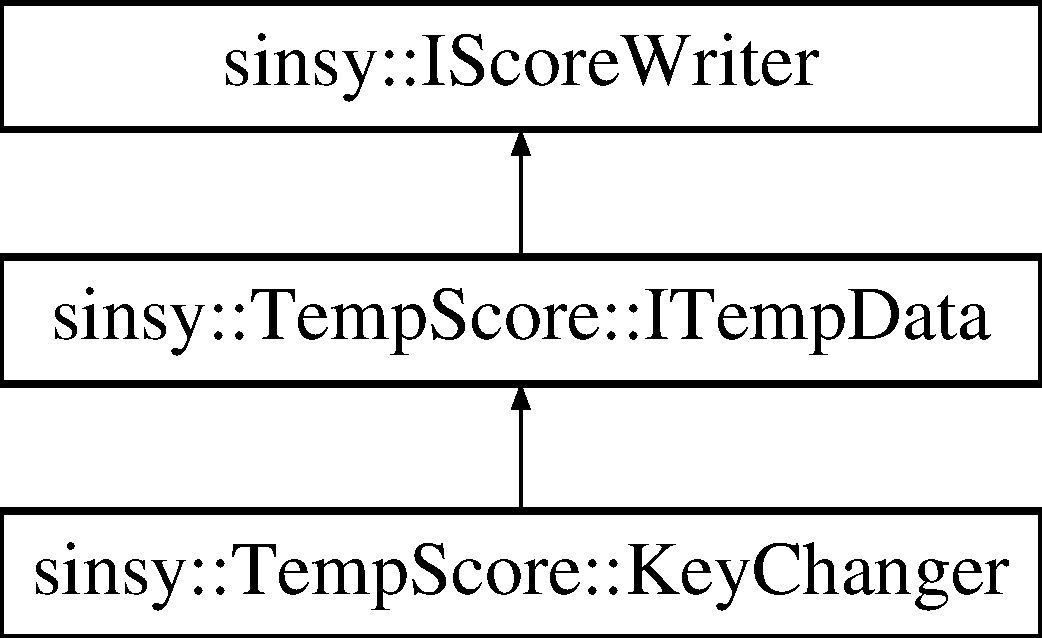
\includegraphics[height=3.000000cm]{classsinsy_1_1TempScore_1_1KeyChanger}
\end{center}
\end{figure}
\subsection*{\-Public \-Member \-Functions}
\begin{DoxyCompactItemize}
\item 
\hypertarget{classsinsy_1_1TempScore_1_1KeyChanger_a8d8f6353b6f163c9c46c974f21bbfe9c}{\hyperlink{classsinsy_1_1TempScore_1_1KeyChanger_a8d8f6353b6f163c9c46c974f21bbfe9c}{\-Key\-Changer} (const \hyperlink{classsinsy_1_1Key}{\-Key} \&k)}\label{classsinsy_1_1TempScore_1_1KeyChanger_a8d8f6353b6f163c9c46c974f21bbfe9c}

\begin{DoxyCompactList}\small\item\em constructor \end{DoxyCompactList}\item 
\hypertarget{classsinsy_1_1TempScore_1_1KeyChanger_a4a5d10d5e35c4d0b35ccbb78a1138c15}{virtual \hyperlink{classsinsy_1_1TempScore_1_1KeyChanger_a4a5d10d5e35c4d0b35ccbb78a1138c15}{$\sim$\-Key\-Changer} ()}\label{classsinsy_1_1TempScore_1_1KeyChanger_a4a5d10d5e35c4d0b35ccbb78a1138c15}

\begin{DoxyCompactList}\small\item\em destructor \end{DoxyCompactList}\item 
\hypertarget{classsinsy_1_1TempScore_1_1KeyChanger_ad20a205bd670d8850a53ab8093fbd78b}{virtual void \hyperlink{classsinsy_1_1TempScore_1_1KeyChanger_ad20a205bd670d8850a53ab8093fbd78b}{write} (\hyperlink{classsinsy_1_1IScoreWritable}{\-I\-Score\-Writable} \&sm) const }\label{classsinsy_1_1TempScore_1_1KeyChanger_ad20a205bd670d8850a53ab8093fbd78b}

\begin{DoxyCompactList}\small\item\em write \end{DoxyCompactList}\end{DoxyCompactItemize}


\-The documentation for this class was generated from the following files\-:\begin{DoxyCompactItemize}
\item 
lib/temporary/\-Temp\-Score.\-h\item 
lib/temporary/\-Temp\-Score.\-cpp\end{DoxyCompactItemize}

\hypertarget{classsinsy_1_1LabelData}{\section{sinsy\-:\-:\-Label\-Data \-Class \-Reference}
\label{classsinsy_1_1LabelData}\index{sinsy\-::\-Label\-Data@{sinsy\-::\-Label\-Data}}
}
\subsection*{\-Public \-Member \-Functions}
\begin{DoxyCompactItemize}
\item 
\hypertarget{classsinsy_1_1LabelData_a68573aaeba9e7e5d2d98bfd9fdb1bcc8}{\hyperlink{classsinsy_1_1LabelData_a68573aaeba9e7e5d2d98bfd9fdb1bcc8}{\-Label\-Data} ()}\label{classsinsy_1_1LabelData_a68573aaeba9e7e5d2d98bfd9fdb1bcc8}

\begin{DoxyCompactList}\small\item\em constructor \end{DoxyCompactList}\item 
\hypertarget{classsinsy_1_1LabelData_a9b33df6f235f7e43eac701e3ff4b5260}{virtual \hyperlink{classsinsy_1_1LabelData_a9b33df6f235f7e43eac701e3ff4b5260}{$\sim$\-Label\-Data} ()}\label{classsinsy_1_1LabelData_a9b33df6f235f7e43eac701e3ff4b5260}

\begin{DoxyCompactList}\small\item\em destructor \end{DoxyCompactList}\item 
\hypertarget{classsinsy_1_1LabelData_a55b78f427ad14ef9a7d6a16f8e0db04d}{void \hyperlink{classsinsy_1_1LabelData_a55b78f427ad14ef9a7d6a16f8e0db04d}{set\-Monophone\-Flag} (bool b)}\label{classsinsy_1_1LabelData_a55b78f427ad14ef9a7d6a16f8e0db04d}

\begin{DoxyCompactList}\small\item\em set monophone flag \end{DoxyCompactList}\item 
void \hyperlink{classsinsy_1_1LabelData_a17f2cfa54ff494875c2ea8f882515dca}{set\-Output\-Time\-Flag} (bool b)
\begin{DoxyCompactList}\small\item\em set output time flag \end{DoxyCompactList}\item 
\hypertarget{classsinsy_1_1LabelData_a16f6284914f7d1ce0dd47363d9cd0c96}{void \hyperlink{classsinsy_1_1LabelData_a16f6284914f7d1ce0dd47363d9cd0c96}{set\-Begin\-Time} (double d)}\label{classsinsy_1_1LabelData_a16f6284914f7d1ce0dd47363d9cd0c96}

\begin{DoxyCompactList}\small\item\em set begin time \end{DoxyCompactList}\item 
\hypertarget{classsinsy_1_1LabelData_aad4e88d3c0b7f4a86409483a89973b14}{void \hyperlink{classsinsy_1_1LabelData_aad4e88d3c0b7f4a86409483a89973b14}{set\-End\-Time} (double d)}\label{classsinsy_1_1LabelData_aad4e88d3c0b7f4a86409483a89973b14}

\begin{DoxyCompactList}\small\item\em set end time \end{DoxyCompactList}\item 
{\footnotesize template$<$class T $>$ }\\void \hyperlink{classsinsy_1_1LabelData_a6f9cfcd19a9265d201be26df961c4e1e}{set} (char category, size\-\_\-t number, const \-T \&)
\begin{DoxyCompactList}\small\item\em set label data \end{DoxyCompactList}\item 
const std\-::string \& \hyperlink{classsinsy_1_1LabelData_ae27b8db2dc06becc0b029029ffbec1f4}{get} (char category, size\-\_\-t number) const 
\begin{DoxyCompactList}\small\item\em get label data \end{DoxyCompactList}\item 
{\footnotesize template$<$$>$ }\\void \hyperlink{classsinsy_1_1LabelData_adc696bf515a05f46a2c5dc33650025ae}{set} (char category, size\-\_\-t number, const bool \&value)
\item 
\hypertarget{classsinsy_1_1LabelData_adc696bf515a05f46a2c5dc33650025ae}{{\footnotesize template$<$$>$ }\\void \hyperlink{classsinsy_1_1LabelData_adc696bf515a05f46a2c5dc33650025ae}{set} (char category, size\-\_\-t number, const bool \&value)}\label{classsinsy_1_1LabelData_adc696bf515a05f46a2c5dc33650025ae}

\begin{DoxyCompactList}\small\item\em set data (bool) \end{DoxyCompactList}\end{DoxyCompactItemize}
\subsection*{\-Friends}
\begin{DoxyCompactItemize}
\item 
\hypertarget{classsinsy_1_1LabelData_af87d1fea4dd91d0cb4212ded5063f43a}{std\-::ostream \& \hyperlink{classsinsy_1_1LabelData_af87d1fea4dd91d0cb4212ded5063f43a}{operator$<$$<$} (std\-::ostream \&, const \hyperlink{classsinsy_1_1LabelData}{\-Label\-Data} \&)}\label{classsinsy_1_1LabelData_af87d1fea4dd91d0cb4212ded5063f43a}

\begin{DoxyCompactList}\small\item\em to stream \end{DoxyCompactList}\end{DoxyCompactItemize}


\subsection{\-Member \-Function \-Documentation}
\hypertarget{classsinsy_1_1LabelData_ae27b8db2dc06becc0b029029ffbec1f4}{\index{sinsy\-::\-Label\-Data@{sinsy\-::\-Label\-Data}!get@{get}}
\index{get@{get}!sinsy::LabelData@{sinsy\-::\-Label\-Data}}
\subsubsection[{get}]{\setlength{\rightskip}{0pt plus 5cm}const std\-::string \& {\bf \-Label\-Data\-::get} (
\begin{DoxyParamCaption}
\item[{char}]{category, }
\item[{size\-\_\-t}]{number}
\end{DoxyParamCaption}
) const}}\label{classsinsy_1_1LabelData_ae27b8db2dc06becc0b029029ffbec1f4}


get label data 

get data \hypertarget{classsinsy_1_1LabelData_a6f9cfcd19a9265d201be26df961c4e1e}{\index{sinsy\-::\-Label\-Data@{sinsy\-::\-Label\-Data}!set@{set}}
\index{set@{set}!sinsy::LabelData@{sinsy\-::\-Label\-Data}}
\subsubsection[{set}]{\setlength{\rightskip}{0pt plus 5cm}template$<$class T $>$ void {\bf sinsy\-::\-Label\-Data\-::set} (
\begin{DoxyParamCaption}
\item[{char}]{category, }
\item[{size\-\_\-t}]{number, }
\item[{const \-T \&}]{value}
\end{DoxyParamCaption}
)}}\label{classsinsy_1_1LabelData_a6f9cfcd19a9265d201be26df961c4e1e}


set label data 

set data \hypertarget{classsinsy_1_1LabelData_adc696bf515a05f46a2c5dc33650025ae}{\index{sinsy\-::\-Label\-Data@{sinsy\-::\-Label\-Data}!set@{set}}
\index{set@{set}!sinsy::LabelData@{sinsy\-::\-Label\-Data}}
\subsubsection[{set}]{\setlength{\rightskip}{0pt plus 5cm}template$<$$>$ void {\bf sinsy\-::\-Label\-Data\-::set} (
\begin{DoxyParamCaption}
\item[{char}]{category, }
\item[{size\-\_\-t}]{number, }
\item[{const bool \&}]{value}
\end{DoxyParamCaption}
)}}\label{classsinsy_1_1LabelData_adc696bf515a05f46a2c5dc33650025ae}
set data (bool) \hypertarget{classsinsy_1_1LabelData_a17f2cfa54ff494875c2ea8f882515dca}{\index{sinsy\-::\-Label\-Data@{sinsy\-::\-Label\-Data}!set\-Output\-Time\-Flag@{set\-Output\-Time\-Flag}}
\index{set\-Output\-Time\-Flag@{set\-Output\-Time\-Flag}!sinsy::LabelData@{sinsy\-::\-Label\-Data}}
\subsubsection[{set\-Output\-Time\-Flag}]{\setlength{\rightskip}{0pt plus 5cm}void {\bf \-Label\-Data\-::set\-Output\-Time\-Flag} (
\begin{DoxyParamCaption}
\item[{bool}]{b}
\end{DoxyParamCaption}
)}}\label{classsinsy_1_1LabelData_a17f2cfa54ff494875c2ea8f882515dca}


set output time flag 

set output flag 

\-The documentation for this class was generated from the following files\-:\begin{DoxyCompactItemize}
\item 
lib/label/\-Label\-Data.\-h\item 
lib/label/\-Label\-Data.\-cpp\end{DoxyCompactItemize}

\hypertarget{classsinsy_1_1LabelMaker}{\section{sinsy\-:\-:\-Label\-Maker \-Class \-Reference}
\label{classsinsy_1_1LabelMaker}\index{sinsy\-::\-Label\-Maker@{sinsy\-::\-Label\-Maker}}
}
\-Inheritance diagram for sinsy\-:\-:\-Label\-Maker\-:\begin{figure}[H]
\begin{center}
\leavevmode
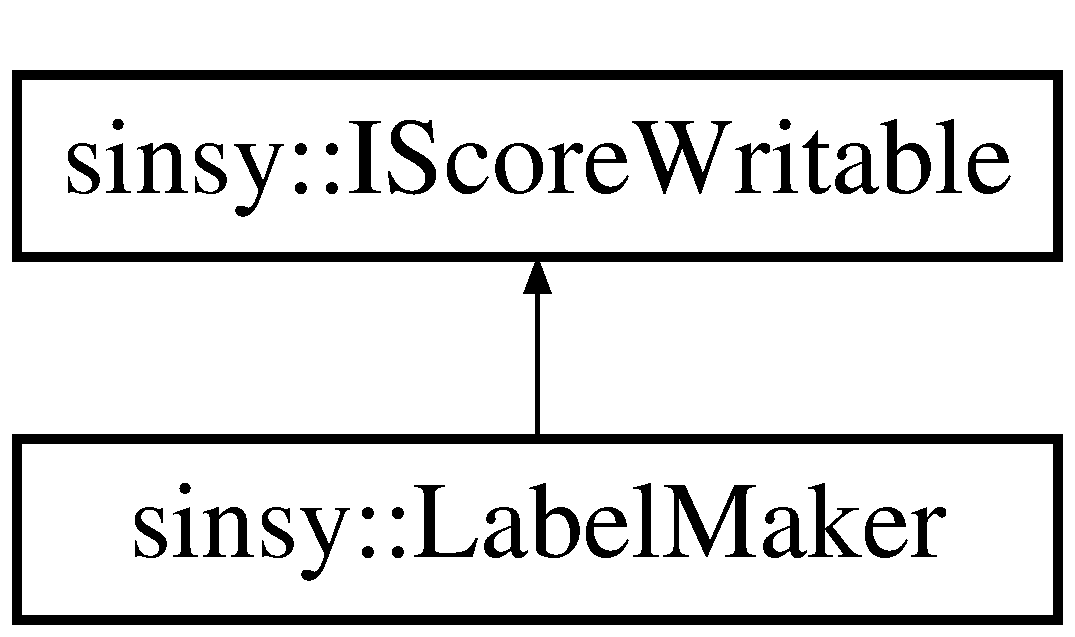
\includegraphics[height=2.000000cm]{classsinsy_1_1LabelMaker}
\end{center}
\end{figure}
\subsection*{\-Public \-Member \-Functions}
\begin{DoxyCompactItemize}
\item 
\hypertarget{classsinsy_1_1LabelMaker_adb707f0e1edc6a3137b8468878b1fca6}{\hyperlink{classsinsy_1_1LabelMaker_adb707f0e1edc6a3137b8468878b1fca6}{\-Label\-Maker} (\hyperlink{classsinsy_1_1Converter}{\-Converter} \&converter, bool sep\-Rests=true)}\label{classsinsy_1_1LabelMaker_adb707f0e1edc6a3137b8468878b1fca6}

\begin{DoxyCompactList}\small\item\em constructor \end{DoxyCompactList}\item 
\hypertarget{classsinsy_1_1LabelMaker_a2d52840e342de1accafd1f44a5641854}{virtual \hyperlink{classsinsy_1_1LabelMaker_a2d52840e342de1accafd1f44a5641854}{$\sim$\-Label\-Maker} ()}\label{classsinsy_1_1LabelMaker_a2d52840e342de1accafd1f44a5641854}

\begin{DoxyCompactList}\small\item\em destructor \end{DoxyCompactList}\item 
\hypertarget{classsinsy_1_1LabelMaker_a978e61679f89b990d5d796847bd750c1}{virtual void \hyperlink{classsinsy_1_1LabelMaker_a978e61679f89b990d5d796847bd750c1}{set\-Encoding} (const std\-::string \&e)}\label{classsinsy_1_1LabelMaker_a978e61679f89b990d5d796847bd750c1}

\begin{DoxyCompactList}\small\item\em set encoding \end{DoxyCompactList}\item 
\hypertarget{classsinsy_1_1LabelMaker_a278703b8ec92253e3095c0d6e98edc9b}{virtual void \hyperlink{classsinsy_1_1LabelMaker_a278703b8ec92253e3095c0d6e98edc9b}{change\-Tempo} (double t)}\label{classsinsy_1_1LabelMaker_a278703b8ec92253e3095c0d6e98edc9b}

\begin{DoxyCompactList}\small\item\em change tempo \end{DoxyCompactList}\item 
\hypertarget{classsinsy_1_1LabelMaker_a6864d59e45b4b06678950d40a9bfc3cc}{virtual void \hyperlink{classsinsy_1_1LabelMaker_a6864d59e45b4b06678950d40a9bfc3cc}{change\-Beat} (const \hyperlink{classsinsy_1_1Beat}{\-Beat} \&b)}\label{classsinsy_1_1LabelMaker_a6864d59e45b4b06678950d40a9bfc3cc}

\begin{DoxyCompactList}\small\item\em change beat \end{DoxyCompactList}\item 
\hypertarget{classsinsy_1_1LabelMaker_aad6773bea2306fc1e6fab5993d090f88}{virtual void \hyperlink{classsinsy_1_1LabelMaker_aad6773bea2306fc1e6fab5993d090f88}{change\-Dynamics} (const \hyperlink{classsinsy_1_1Dynamics}{\-Dynamics} \&d)}\label{classsinsy_1_1LabelMaker_aad6773bea2306fc1e6fab5993d090f88}

\begin{DoxyCompactList}\small\item\em change dynamics \end{DoxyCompactList}\item 
\hypertarget{classsinsy_1_1LabelMaker_ae848767fe7964e6d890ea5f739bd8638}{virtual void \hyperlink{classsinsy_1_1LabelMaker_ae848767fe7964e6d890ea5f739bd8638}{change\-Key} (const \hyperlink{classsinsy_1_1Key}{\-Key} \&k)}\label{classsinsy_1_1LabelMaker_ae848767fe7964e6d890ea5f739bd8638}

\begin{DoxyCompactList}\small\item\em change key \end{DoxyCompactList}\item 
\hypertarget{classsinsy_1_1LabelMaker_aae52e30f45a9e50d19e0d7ee3ccf9035}{virtual void \hyperlink{classsinsy_1_1LabelMaker_aae52e30f45a9e50d19e0d7ee3ccf9035}{start\-Crescendo} ()}\label{classsinsy_1_1LabelMaker_aae52e30f45a9e50d19e0d7ee3ccf9035}

\begin{DoxyCompactList}\small\item\em start crescendo \end{DoxyCompactList}\item 
\hypertarget{classsinsy_1_1LabelMaker_a8bd2cef4cbd551739b7973c570d6b70f}{virtual void \hyperlink{classsinsy_1_1LabelMaker_a8bd2cef4cbd551739b7973c570d6b70f}{start\-Diminuendo} ()}\label{classsinsy_1_1LabelMaker_a8bd2cef4cbd551739b7973c570d6b70f}

\begin{DoxyCompactList}\small\item\em start diminuendo \end{DoxyCompactList}\item 
\hypertarget{classsinsy_1_1LabelMaker_a8bc2f4dd586aa8e89cb790560e1b9c01}{virtual void \hyperlink{classsinsy_1_1LabelMaker_a8bc2f4dd586aa8e89cb790560e1b9c01}{stop\-Crescendo} ()}\label{classsinsy_1_1LabelMaker_a8bc2f4dd586aa8e89cb790560e1b9c01}

\begin{DoxyCompactList}\small\item\em stop crescendo \end{DoxyCompactList}\item 
\hypertarget{classsinsy_1_1LabelMaker_abd05f88c778af183152fb451ffdb3ead}{virtual void \hyperlink{classsinsy_1_1LabelMaker_abd05f88c778af183152fb451ffdb3ead}{stop\-Diminuendo} ()}\label{classsinsy_1_1LabelMaker_abd05f88c778af183152fb451ffdb3ead}

\begin{DoxyCompactList}\small\item\em stop diminuendo \end{DoxyCompactList}\item 
\hypertarget{classsinsy_1_1LabelMaker_a10e05c4a3659934bab28afa9da526485}{virtual void \hyperlink{classsinsy_1_1LabelMaker_a10e05c4a3659934bab28afa9da526485}{add\-Note} (const \hyperlink{classsinsy_1_1Note}{\-Note} \&note)}\label{classsinsy_1_1LabelMaker_a10e05c4a3659934bab28afa9da526485}

\begin{DoxyCompactList}\small\item\em add note \end{DoxyCompactList}\item 
\hypertarget{classsinsy_1_1LabelMaker_a4693a701ba327d990576ed695476b2d9}{void \hyperlink{classsinsy_1_1LabelMaker_a4693a701ba327d990576ed695476b2d9}{fix} ()}\label{classsinsy_1_1LabelMaker_a4693a701ba327d990576ed695476b2d9}

\begin{DoxyCompactList}\small\item\em fix \end{DoxyCompactList}\item 
\hypertarget{classsinsy_1_1LabelMaker_a417030b25b59f3d6404c4a6dbe91a76b}{void \hyperlink{classsinsy_1_1LabelMaker_a417030b25b59f3d6404c4a6dbe91a76b}{output\-Label} (\hyperlink{classsinsy_1_1ILabelOutput}{\-I\-Label\-Output} \&output, bool monophone\-Flag=false, int overwrite\-Enable\-Flag=0, int time\-Flag=0) const }\label{classsinsy_1_1LabelMaker_a417030b25b59f3d6404c4a6dbe91a76b}

\begin{DoxyCompactList}\small\item\em output label \end{DoxyCompactList}\end{DoxyCompactItemize}


\-The documentation for this class was generated from the following files\-:\begin{DoxyCompactItemize}
\item 
lib/label/\-Label\-Maker.\-h\item 
lib/label/\-Label\-Maker.\-cpp\end{DoxyCompactItemize}

\hypertarget{classsinsy_1_1LabelMeasure}{\section{sinsy\-:\-:\-Label\-Measure \-Class \-Reference}
\label{classsinsy_1_1LabelMeasure}\index{sinsy\-::\-Label\-Measure@{sinsy\-::\-Label\-Measure}}
}
\subsection*{\-Public \-Member \-Functions}
\begin{DoxyCompactItemize}
\item 
\hypertarget{classsinsy_1_1LabelMeasure_ad780a2297ee5784a5c790c520f682702}{\hyperlink{classsinsy_1_1LabelMeasure_ad780a2297ee5784a5c790c520f682702}{\-Label\-Measure} (const \hyperlink{classsinsy_1_1Beat}{\-Beat} \&b)}\label{classsinsy_1_1LabelMeasure_ad780a2297ee5784a5c790c520f682702}

\begin{DoxyCompactList}\small\item\em constructor \end{DoxyCompactList}\item 
\hypertarget{classsinsy_1_1LabelMeasure_abb53c4d1bf440d1e4eceafaedf40291c}{virtual \hyperlink{classsinsy_1_1LabelMeasure_abb53c4d1bf440d1e4eceafaedf40291c}{$\sim$\-Label\-Measure} ()}\label{classsinsy_1_1LabelMeasure_abb53c4d1bf440d1e4eceafaedf40291c}

\begin{DoxyCompactList}\small\item\em destructor \end{DoxyCompactList}\item 
\hypertarget{classsinsy_1_1LabelMeasure_a1b1d02be7c077632a4b5ec957d0accf6}{void \hyperlink{classsinsy_1_1LabelMeasure_a1b1d02be7c077632a4b5ec957d0accf6}{add\-Position} (const \hyperlink{classsinsy_1_1LabelPosition}{\-Label\-Position} \&)}\label{classsinsy_1_1LabelMeasure_a1b1d02be7c077632a4b5ec957d0accf6}

\begin{DoxyCompactList}\small\item\em add position \end{DoxyCompactList}\item 
\hypertarget{classsinsy_1_1LabelMeasure_a590b720a524ad907302d97d91faf8d1d}{const \hyperlink{classsinsy_1_1LabelPosition}{\-Label\-Position} \& \hyperlink{classsinsy_1_1LabelMeasure_a590b720a524ad907302d97d91faf8d1d}{get\-Position} () const }\label{classsinsy_1_1LabelMeasure_a590b720a524ad907302d97d91faf8d1d}

\begin{DoxyCompactList}\small\item\em get position \end{DoxyCompactList}\item 
\hypertarget{classsinsy_1_1LabelMeasure_ac4908cfa8d721d71db8458bc7b978f49}{void \hyperlink{classsinsy_1_1LabelMeasure_ac4908cfa8d721d71db8458bc7b978f49}{set\-Max\-Position} (const \hyperlink{classsinsy_1_1LabelPosition}{\-Label\-Position} \&)}\label{classsinsy_1_1LabelMeasure_ac4908cfa8d721d71db8458bc7b978f49}

\begin{DoxyCompactList}\small\item\em set max position \end{DoxyCompactList}\item 
\hypertarget{classsinsy_1_1LabelMeasure_ad475e134e4ee84343e1217f63092f56c}{const \hyperlink{classsinsy_1_1LabelPosition}{\-Label\-Position} \& \hyperlink{classsinsy_1_1LabelMeasure_ad475e134e4ee84343e1217f63092f56c}{get\-Max\-Position} () const }\label{classsinsy_1_1LabelMeasure_ad475e134e4ee84343e1217f63092f56c}

\begin{DoxyCompactList}\small\item\em get max position \end{DoxyCompactList}\item 
\hypertarget{classsinsy_1_1LabelMeasure_a5105945476e55d5d94e8aaeb9425f052}{const \-I\-N\-T64 \hyperlink{classsinsy_1_1LabelMeasure_a5105945476e55d5d94e8aaeb9425f052}{get\-Duration} () const }\label{classsinsy_1_1LabelMeasure_a5105945476e55d5d94e8aaeb9425f052}

\begin{DoxyCompactList}\small\item\em get duration \end{DoxyCompactList}\end{DoxyCompactItemize}


\-The documentation for this class was generated from the following files\-:\begin{DoxyCompactItemize}
\item 
lib/label/\-Label\-Measure.\-h\item 
lib/label/\-Label\-Measure.\-cpp\end{DoxyCompactItemize}

\hypertarget{classsinsy_1_1LabelPosition}{\section{sinsy\-:\-:\-Label\-Position \-Class \-Reference}
\label{classsinsy_1_1LabelPosition}\index{sinsy\-::\-Label\-Position@{sinsy\-::\-Label\-Position}}
}
\subsection*{\-Public \-Member \-Functions}
\begin{DoxyCompactItemize}
\item 
\hypertarget{classsinsy_1_1LabelPosition_a6a6261add8f0bb184176adfa6b928d19}{\hyperlink{classsinsy_1_1LabelPosition_a6a6261add8f0bb184176adfa6b928d19}{\-Label\-Position} ()}\label{classsinsy_1_1LabelPosition_a6a6261add8f0bb184176adfa6b928d19}

\begin{DoxyCompactList}\small\item\em constructor \end{DoxyCompactList}\item 
\hypertarget{classsinsy_1_1LabelPosition_a83dbcb24442688d370b5368dca02d969}{\hyperlink{classsinsy_1_1LabelPosition_a83dbcb24442688d370b5368dca02d969}{\-Label\-Position} (size\-\_\-t dur, double tempo)}\label{classsinsy_1_1LabelPosition_a83dbcb24442688d370b5368dca02d969}

\begin{DoxyCompactList}\small\item\em constructor \end{DoxyCompactList}\item 
\hypertarget{classsinsy_1_1LabelPosition_a3fc2b14b2710f75beff7db2e216c9f96}{\hyperlink{classsinsy_1_1LabelPosition_a3fc2b14b2710f75beff7db2e216c9f96}{\-Label\-Position} (const \hyperlink{classsinsy_1_1LabelPosition}{\-Label\-Position} \&obj)}\label{classsinsy_1_1LabelPosition_a3fc2b14b2710f75beff7db2e216c9f96}

\begin{DoxyCompactList}\small\item\em copy constructor \end{DoxyCompactList}\item 
\hypertarget{classsinsy_1_1LabelPosition_a8d20aa75f5cc895fe5f3e2b93bc418c6}{virtual \hyperlink{classsinsy_1_1LabelPosition_a8d20aa75f5cc895fe5f3e2b93bc418c6}{$\sim$\-Label\-Position} ()}\label{classsinsy_1_1LabelPosition_a8d20aa75f5cc895fe5f3e2b93bc418c6}

\begin{DoxyCompactList}\small\item\em destructor \end{DoxyCompactList}\item 
\hypertarget{classsinsy_1_1LabelPosition_aa399e69f3337b88c768e574350bf2274}{\hyperlink{classsinsy_1_1LabelPosition}{\-Label\-Position} \& \hyperlink{classsinsy_1_1LabelPosition_aa399e69f3337b88c768e574350bf2274}{operator=} (const \hyperlink{classsinsy_1_1LabelPosition}{\-Label\-Position} \&obj)}\label{classsinsy_1_1LabelPosition_aa399e69f3337b88c768e574350bf2274}

\begin{DoxyCompactList}\small\item\em assignment operator \end{DoxyCompactList}\item 
\hypertarget{classsinsy_1_1LabelPosition_a1c30e2a6a0a41941ac016b265c3f6c39}{\hyperlink{classsinsy_1_1LabelPosition}{\-Label\-Position} \& \hyperlink{classsinsy_1_1LabelPosition_a1c30e2a6a0a41941ac016b265c3f6c39}{operator+=} (const \hyperlink{classsinsy_1_1LabelPosition}{\-Label\-Position} \&obj)}\label{classsinsy_1_1LabelPosition_a1c30e2a6a0a41941ac016b265c3f6c39}

\begin{DoxyCompactList}\small\item\em operator += \end{DoxyCompactList}\item 
\hypertarget{classsinsy_1_1LabelPosition_aafd20041d722265ba62dcae6c46a0dd2}{\hyperlink{classsinsy_1_1LabelPosition}{\-Label\-Position} \& \hyperlink{classsinsy_1_1LabelPosition_aafd20041d722265ba62dcae6c46a0dd2}{operator-\/=} (const \hyperlink{classsinsy_1_1LabelPosition}{\-Label\-Position} \&obj)}\label{classsinsy_1_1LabelPosition_aafd20041d722265ba62dcae6c46a0dd2}

\begin{DoxyCompactList}\small\item\em operator -\/= \end{DoxyCompactList}\item 
\hypertarget{classsinsy_1_1LabelPosition_a7c3ff6672f9ae612a88d6e1bacfcf759}{\hyperlink{classsinsy_1_1LabelPosition}{\-Label\-Position} \hyperlink{classsinsy_1_1LabelPosition_a7c3ff6672f9ae612a88d6e1bacfcf759}{operator+} (const \hyperlink{classsinsy_1_1LabelPosition}{\-Label\-Position} \&) const }\label{classsinsy_1_1LabelPosition_a7c3ff6672f9ae612a88d6e1bacfcf759}

\begin{DoxyCompactList}\small\item\em operator + \end{DoxyCompactList}\item 
\hypertarget{classsinsy_1_1LabelPosition_ac4c23a1f9a09fbee0ea87779a8640ee8}{\hyperlink{classsinsy_1_1LabelPosition}{\-Label\-Position} \hyperlink{classsinsy_1_1LabelPosition_ac4c23a1f9a09fbee0ea87779a8640ee8}{operator-\/} (const \hyperlink{classsinsy_1_1LabelPosition}{\-Label\-Position} \&) const }\label{classsinsy_1_1LabelPosition_ac4c23a1f9a09fbee0ea87779a8640ee8}

\begin{DoxyCompactList}\small\item\em operator -\/ \end{DoxyCompactList}\item 
\hypertarget{classsinsy_1_1LabelPosition_a6c3352ba3c0a713af78e63ad7e666781}{void \hyperlink{classsinsy_1_1LabelPosition_a6c3352ba3c0a713af78e63ad7e666781}{add} (size\-\_\-t dur, double tempo)}\label{classsinsy_1_1LabelPosition_a6c3352ba3c0a713af78e63ad7e666781}

\begin{DoxyCompactList}\small\item\em add \end{DoxyCompactList}\item 
\hypertarget{classsinsy_1_1LabelPosition_ac17e76f3924c3d30bb5e100266c7278e}{void \hyperlink{classsinsy_1_1LabelPosition_ac17e76f3924c3d30bb5e100266c7278e}{set\-Count} (size\-\_\-t c)}\label{classsinsy_1_1LabelPosition_ac17e76f3924c3d30bb5e100266c7278e}

\begin{DoxyCompactList}\small\item\em set count \end{DoxyCompactList}\item 
\hypertarget{classsinsy_1_1LabelPosition_a4a0f876b71e59bc08e274ac34de3c380}{\-I\-N\-T64 \hyperlink{classsinsy_1_1LabelPosition_a4a0f876b71e59bc08e274ac34de3c380}{get\-Count} () const }\label{classsinsy_1_1LabelPosition_a4a0f876b71e59bc08e274ac34de3c380}

\begin{DoxyCompactList}\small\item\em get count \end{DoxyCompactList}\item 
\hypertarget{classsinsy_1_1LabelPosition_ad90033db8d7524d7a0011dc3890e390a}{double \hyperlink{classsinsy_1_1LabelPosition_ad90033db8d7524d7a0011dc3890e390a}{get\-Time} () const }\label{classsinsy_1_1LabelPosition_ad90033db8d7524d7a0011dc3890e390a}

\begin{DoxyCompactList}\small\item\em get time \end{DoxyCompactList}\item 
\hypertarget{classsinsy_1_1LabelPosition_ad6de4e3d600db95a5af0a5d76832457c}{\-I\-N\-T64 \hyperlink{classsinsy_1_1LabelPosition_ad6de4e3d600db95a5af0a5d76832457c}{get\-Point} () const }\label{classsinsy_1_1LabelPosition_ad6de4e3d600db95a5af0a5d76832457c}

\begin{DoxyCompactList}\small\item\em get point \end{DoxyCompactList}\item 
\hypertarget{classsinsy_1_1LabelPosition_aadd9dc47070a0adf3f1fbc62bc7bcddc}{\-I\-N\-T64 \hyperlink{classsinsy_1_1LabelPosition_aadd9dc47070a0adf3f1fbc62bc7bcddc}{get\-Duration} () const }\label{classsinsy_1_1LabelPosition_aadd9dc47070a0adf3f1fbc62bc7bcddc}

\begin{DoxyCompactList}\small\item\em get duration \end{DoxyCompactList}\end{DoxyCompactItemize}


\-The documentation for this class was generated from the following files\-:\begin{DoxyCompactItemize}
\item 
lib/label/\-Label\-Position.\-h\item 
lib/label/\-Label\-Position.\-cpp\end{DoxyCompactItemize}

\hypertarget{classsinsy_1_1LabelStream}{\section{sinsy\-:\-:\-Label\-Stream \-Class \-Reference}
\label{classsinsy_1_1LabelStream}\index{sinsy\-::\-Label\-Stream@{sinsy\-::\-Label\-Stream}}
}
\-Inheritance diagram for sinsy\-:\-:\-Label\-Stream\-:\begin{figure}[H]
\begin{center}
\leavevmode
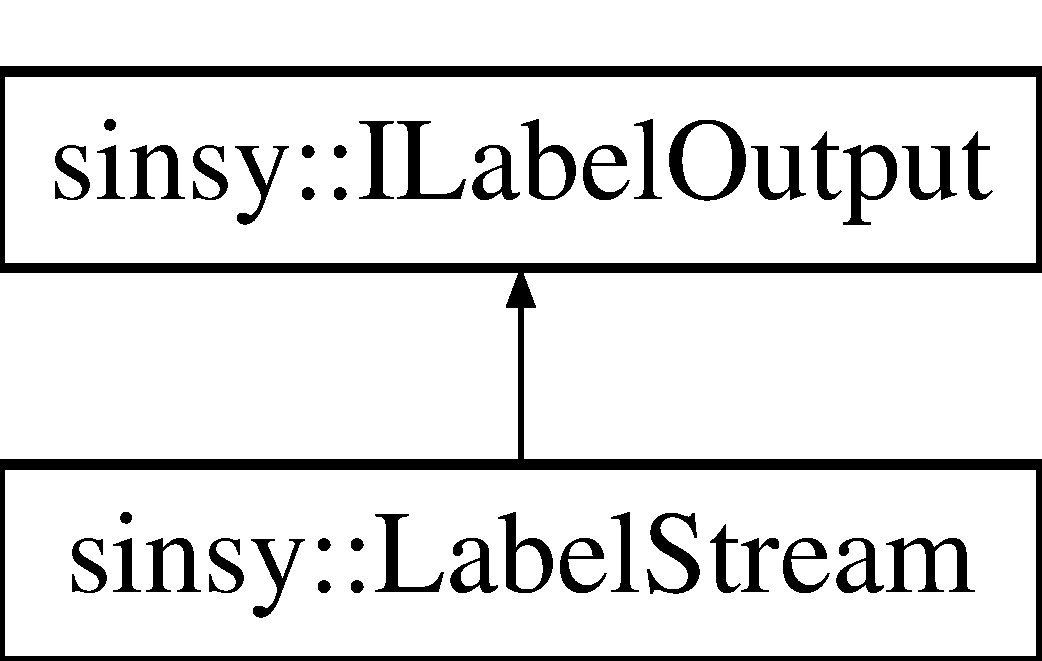
\includegraphics[height=2.000000cm]{classsinsy_1_1LabelStream}
\end{center}
\end{figure}
\subsection*{\-Public \-Member \-Functions}
\begin{DoxyCompactItemize}
\item 
\hypertarget{classsinsy_1_1LabelStream_a8472d56cb16d61cc3b0f6c45db368f25}{\hyperlink{classsinsy_1_1LabelStream_a8472d56cb16d61cc3b0f6c45db368f25}{\-Label\-Stream} (std\-::ostream \&os)}\label{classsinsy_1_1LabelStream_a8472d56cb16d61cc3b0f6c45db368f25}

\begin{DoxyCompactList}\small\item\em constructor \end{DoxyCompactList}\item 
\hypertarget{classsinsy_1_1LabelStream_a6afb2fa70bb9c1c961cce597d7a28911}{virtual \hyperlink{classsinsy_1_1LabelStream_a6afb2fa70bb9c1c961cce597d7a28911}{$\sim$\-Label\-Stream} ()}\label{classsinsy_1_1LabelStream_a6afb2fa70bb9c1c961cce597d7a28911}

\begin{DoxyCompactList}\small\item\em destructor \end{DoxyCompactList}\item 
virtual void \hyperlink{classsinsy_1_1LabelStream_a594f1eb2ba94797e7b7fa595c215fc46}{output} (const std\-::string \&)
\begin{DoxyCompactList}\small\item\em output label \end{DoxyCompactList}\end{DoxyCompactItemize}


\subsection{\-Member \-Function \-Documentation}
\hypertarget{classsinsy_1_1LabelStream_a594f1eb2ba94797e7b7fa595c215fc46}{\index{sinsy\-::\-Label\-Stream@{sinsy\-::\-Label\-Stream}!output@{output}}
\index{output@{output}!sinsy::LabelStream@{sinsy\-::\-Label\-Stream}}
\subsubsection[{output}]{\setlength{\rightskip}{0pt plus 5cm}void {\bf \-Label\-Stream\-::output} (
\begin{DoxyParamCaption}
\item[{const std\-::string \&}]{str}
\end{DoxyParamCaption}
)\hspace{0.3cm}{\ttfamily  \mbox{[}virtual\mbox{]}}}}\label{classsinsy_1_1LabelStream_a594f1eb2ba94797e7b7fa595c215fc46}


output label 

output label


\begin{DoxyParams}{\-Parameters}
{\em str} & label string \\
\hline
\end{DoxyParams}


\-Implements \hyperlink{classsinsy_1_1ILabelOutput_a5ba6152a812e466398a45db0106a11bb}{sinsy\-::\-I\-Label\-Output}.



\-The documentation for this class was generated from the following files\-:\begin{DoxyCompactItemize}
\item 
lib/label/\-Label\-Stream.\-h\item 
lib/label/\-Label\-Stream.\-cpp\end{DoxyCompactItemize}

\hypertarget{classsinsy_1_1LabelStrings}{\section{sinsy\-:\-:\-Label\-Strings \-Class \-Reference}
\label{classsinsy_1_1LabelStrings}\index{sinsy\-::\-Label\-Strings@{sinsy\-::\-Label\-Strings}}
}
\-Inheritance diagram for sinsy\-:\-:\-Label\-Strings\-:\begin{figure}[H]
\begin{center}
\leavevmode
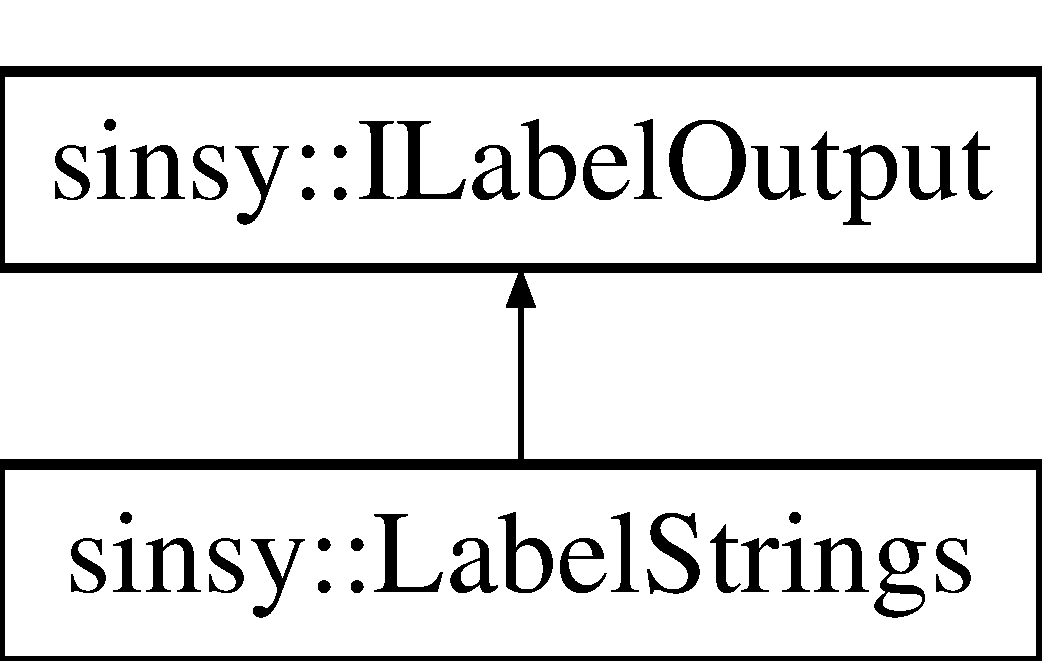
\includegraphics[height=2.000000cm]{classsinsy_1_1LabelStrings}
\end{center}
\end{figure}
\subsection*{\-Public \-Member \-Functions}
\begin{DoxyCompactItemize}
\item 
\hypertarget{classsinsy_1_1LabelStrings_a2fa90f22323d9432cc52626998861954}{\hyperlink{classsinsy_1_1LabelStrings_a2fa90f22323d9432cc52626998861954}{\-Label\-Strings} ()}\label{classsinsy_1_1LabelStrings_a2fa90f22323d9432cc52626998861954}

\begin{DoxyCompactList}\small\item\em constructor \end{DoxyCompactList}\item 
\hypertarget{classsinsy_1_1LabelStrings_a58f7cdd90cf82767508bdf6b25f24805}{virtual \hyperlink{classsinsy_1_1LabelStrings_a58f7cdd90cf82767508bdf6b25f24805}{$\sim$\-Label\-Strings} ()}\label{classsinsy_1_1LabelStrings_a58f7cdd90cf82767508bdf6b25f24805}

\begin{DoxyCompactList}\small\item\em destructor \end{DoxyCompactList}\item 
\hypertarget{classsinsy_1_1LabelStrings_a2269c6943a38c588352963ba7fa6de00}{size\-\_\-t \hyperlink{classsinsy_1_1LabelStrings_a2269c6943a38c588352963ba7fa6de00}{size} () const }\label{classsinsy_1_1LabelStrings_a2269c6943a38c588352963ba7fa6de00}

\begin{DoxyCompactList}\small\item\em get size \end{DoxyCompactList}\item 
\hypertarget{classsinsy_1_1LabelStrings_ae708611dbb4a3fff181a5af6e1723445}{const char $\ast$const $\ast$ \hyperlink{classsinsy_1_1LabelStrings_ae708611dbb4a3fff181a5af6e1723445}{get\-Data} () const }\label{classsinsy_1_1LabelStrings_ae708611dbb4a3fff181a5af6e1723445}

\begin{DoxyCompactList}\small\item\em get data \end{DoxyCompactList}\item 
\hypertarget{classsinsy_1_1LabelStrings_a75d7ede96c667305e7bf40c82d63812a}{virtual void \hyperlink{classsinsy_1_1LabelStrings_a75d7ede96c667305e7bf40c82d63812a}{output} (const std\-::string \&str)}\label{classsinsy_1_1LabelStrings_a75d7ede96c667305e7bf40c82d63812a}

\begin{DoxyCompactList}\small\item\em output label \end{DoxyCompactList}\item 
\hypertarget{classsinsy_1_1LabelStrings_a218e781ed11aa690a11499fd626b077c}{void {\bfseries print\-Labels} (std\-::string fn)}\label{classsinsy_1_1LabelStrings_a218e781ed11aa690a11499fd626b077c}

\end{DoxyCompactItemize}


\-The documentation for this class was generated from the following files\-:\begin{DoxyCompactItemize}
\item 
lib/label/\-Label\-Strings.\-h\item 
lib/label/\-Label\-Strings.\-cpp\end{DoxyCompactItemize}

\hypertarget{classsinsy_1_1MacronTable}{\section{sinsy\-:\-:\-Macron\-Table \-Class \-Reference}
\label{classsinsy_1_1MacronTable}\index{sinsy\-::\-Macron\-Table@{sinsy\-::\-Macron\-Table}}
}
\subsection*{\-Classes}
\begin{DoxyCompactItemize}
\item 
struct {\bfseries \-Result}
\end{DoxyCompactItemize}
\subsection*{\-Public \-Types}
\begin{DoxyCompactItemize}
\item 
\hypertarget{classsinsy_1_1MacronTable_a393cc7c9bbcd3ed7fdb0df6a7971359f}{typedef std\-::vector$<$ std\-::string $>$ {\bfseries \-Phoneme\-List}}\label{classsinsy_1_1MacronTable_a393cc7c9bbcd3ed7fdb0df6a7971359f}

\end{DoxyCompactItemize}
\subsection*{\-Public \-Member \-Functions}
\begin{DoxyCompactItemize}
\item 
\hypertarget{classsinsy_1_1MacronTable_a137cccb1480580ac32f4a680e8896ec6}{\hyperlink{classsinsy_1_1MacronTable_a137cccb1480580ac32f4a680e8896ec6}{\-Macron\-Table} ()}\label{classsinsy_1_1MacronTable_a137cccb1480580ac32f4a680e8896ec6}

\begin{DoxyCompactList}\small\item\em constructor \end{DoxyCompactList}\item 
\hypertarget{classsinsy_1_1MacronTable_a44defde6b551d1e86da4a10df717a8c8}{virtual \hyperlink{classsinsy_1_1MacronTable_a44defde6b551d1e86da4a10df717a8c8}{$\sim$\-Macron\-Table} ()}\label{classsinsy_1_1MacronTable_a44defde6b551d1e86da4a10df717a8c8}

\begin{DoxyCompactList}\small\item\em destructor \end{DoxyCompactList}\item 
\hypertarget{classsinsy_1_1MacronTable_a33de031c61b3728d396a019172e90297}{void \hyperlink{classsinsy_1_1MacronTable_a33de031c61b3728d396a019172e90297}{clear} ()}\label{classsinsy_1_1MacronTable_a33de031c61b3728d396a019172e90297}

\begin{DoxyCompactList}\small\item\em clear \end{DoxyCompactList}\item 
bool \hyperlink{classsinsy_1_1MacronTable_a00ff6032cc6c54767863b428a6c16504}{read} (const std\-::string \&fname)
\begin{DoxyCompactList}\small\item\em read from file \end{DoxyCompactList}\item 
\hypertarget{classsinsy_1_1MacronTable_ad95067afd473b04f25d3eccb957f997f}{bool \hyperlink{classsinsy_1_1MacronTable_ad95067afd473b04f25d3eccb957f997f}{divide} (const \-Phoneme\-List \&src, \-Phoneme\-List \&dst1, \-Phoneme\-List \&dst2) const }\label{classsinsy_1_1MacronTable_ad95067afd473b04f25d3eccb957f997f}

\begin{DoxyCompactList}\small\item\em divide phoneme set \end{DoxyCompactList}\end{DoxyCompactItemize}


\subsection{\-Member \-Function \-Documentation}
\hypertarget{classsinsy_1_1MacronTable_a00ff6032cc6c54767863b428a6c16504}{\index{sinsy\-::\-Macron\-Table@{sinsy\-::\-Macron\-Table}!read@{read}}
\index{read@{read}!sinsy::MacronTable@{sinsy\-::\-Macron\-Table}}
\subsubsection[{read}]{\setlength{\rightskip}{0pt plus 5cm}bool {\bf \-Macron\-Table\-::read} (
\begin{DoxyParamCaption}
\item[{const std\-::string \&}]{fname}
\end{DoxyParamCaption}
)}}\label{classsinsy_1_1MacronTable_a00ff6032cc6c54767863b428a6c16504}


read from file 

read from file

\-If the file is not exist, output warning message and return true.


\begin{DoxyParams}{\-Parameters}
{\em fname} & phoneme table file path \\
\hline
{\em return} & true if success \\
\hline
\end{DoxyParams}


\-The documentation for this class was generated from the following files\-:\begin{DoxyCompactItemize}
\item 
lib/util/\-Macron\-Table.\-h\item 
lib/util/\-Macron\-Table.\-cpp\end{DoxyCompactItemize}

\hypertarget{classsinsy_1_1Mode}{\section{sinsy\-:\-:\-Mode \-Class \-Reference}
\label{classsinsy_1_1Mode}\index{sinsy\-::\-Mode@{sinsy\-::\-Mode}}
}
\subsection*{\-Public \-Member \-Functions}
\begin{DoxyCompactItemize}
\item 
\hypertarget{classsinsy_1_1Mode_a098246baedeee64fa0ed3b53547cf55f}{\hyperlink{classsinsy_1_1Mode_a098246baedeee64fa0ed3b53547cf55f}{\-Mode} ()}\label{classsinsy_1_1Mode_a098246baedeee64fa0ed3b53547cf55f}

\begin{DoxyCompactList}\small\item\em constructor \end{DoxyCompactList}\item 
\hyperlink{classsinsy_1_1Mode_a1b2d5d264bc2de44e9efc27b98fb482c}{\-Mode} (const std\-::string \&str)
\begin{DoxyCompactList}\small\item\em constructor \end{DoxyCompactList}\item 
\hypertarget{classsinsy_1_1Mode_ae7f0ff16a094082d2f9896c077fd6ddf}{\hyperlink{classsinsy_1_1Mode_ae7f0ff16a094082d2f9896c077fd6ddf}{\-Mode} (const \hyperlink{classsinsy_1_1Mode}{\-Mode} \&obj)}\label{classsinsy_1_1Mode_ae7f0ff16a094082d2f9896c077fd6ddf}

\begin{DoxyCompactList}\small\item\em copy constructor \end{DoxyCompactList}\item 
\hypertarget{classsinsy_1_1Mode_a6b8809388084822aeac00adbcbe107f7}{virtual \hyperlink{classsinsy_1_1Mode_a6b8809388084822aeac00adbcbe107f7}{$\sim$\-Mode} ()}\label{classsinsy_1_1Mode_a6b8809388084822aeac00adbcbe107f7}

\begin{DoxyCompactList}\small\item\em destructor \end{DoxyCompactList}\item 
\hypertarget{classsinsy_1_1Mode_ac8122253680690c29f4a48e01d7fef2a}{\hyperlink{classsinsy_1_1Mode}{\-Mode} \& \hyperlink{classsinsy_1_1Mode_ac8122253680690c29f4a48e01d7fef2a}{operator=} (const \hyperlink{classsinsy_1_1Mode}{\-Mode} \&obj)}\label{classsinsy_1_1Mode_ac8122253680690c29f4a48e01d7fef2a}

\begin{DoxyCompactList}\small\item\em assignment operator \end{DoxyCompactList}\item 
bool \hyperlink{classsinsy_1_1Mode_a9a90d9c77d25798d8b4dd3c427a7cd3f}{operator==} (const \hyperlink{classsinsy_1_1Mode}{\-Mode} \&obj) const 
\begin{DoxyCompactList}\small\item\em equal \end{DoxyCompactList}\item 
bool \hyperlink{classsinsy_1_1Mode_a585d85c933d17df58e76a5ce5770a5b8}{operator!=} (const \hyperlink{classsinsy_1_1Mode}{\-Mode} \&obj) const 
\begin{DoxyCompactList}\small\item\em not equal \end{DoxyCompactList}\item 
void \hyperlink{classsinsy_1_1Mode_a406a7630df242c2e2cc0d751d684af32}{set} (const std\-::string \&str)
\begin{DoxyCompactList}\small\item\em set mode \end{DoxyCompactList}\item 
const std\-::string \& \hyperlink{classsinsy_1_1Mode_af6cddd424f3303817245cdc324ef1589}{get} () const 
\begin{DoxyCompactList}\small\item\em get mode \end{DoxyCompactList}\end{DoxyCompactItemize}
\subsection*{\-Static \-Public \-Attributes}
\begin{DoxyCompactItemize}
\item 
\hypertarget{classsinsy_1_1Mode_ae0408cf44be2a33f0da76c9f9500dadf}{static const \hyperlink{classsinsy_1_1Mode}{\-Mode} {\bfseries \-M\-A\-J\-O\-R}}\label{classsinsy_1_1Mode_ae0408cf44be2a33f0da76c9f9500dadf}

\item 
\hypertarget{classsinsy_1_1Mode_a2e0a735ec05a389546ef8c1a2ff8d125}{static const \hyperlink{classsinsy_1_1Mode}{\-Mode} {\bfseries \-M\-I\-N\-O\-R}}\label{classsinsy_1_1Mode_a2e0a735ec05a389546ef8c1a2ff8d125}

\end{DoxyCompactItemize}


\subsection{\-Constructor \& \-Destructor \-Documentation}
\hypertarget{classsinsy_1_1Mode_a1b2d5d264bc2de44e9efc27b98fb482c}{\index{sinsy\-::\-Mode@{sinsy\-::\-Mode}!\-Mode@{\-Mode}}
\index{\-Mode@{\-Mode}!sinsy::Mode@{sinsy\-::\-Mode}}
\subsubsection[{\-Mode}]{\setlength{\rightskip}{0pt plus 5cm}{\bf \-Mode\-::\-Mode} (
\begin{DoxyParamCaption}
\item[{const std\-::string \&}]{str}
\end{DoxyParamCaption}
)\hspace{0.3cm}{\ttfamily  \mbox{[}explicit\mbox{]}}}}\label{classsinsy_1_1Mode_a1b2d5d264bc2de44e9efc27b98fb482c}


constructor 

constructor


\begin{DoxyParams}{\-Parameters}
{\em str} & mode \\
\hline
\end{DoxyParams}


\subsection{\-Member \-Function \-Documentation}
\hypertarget{classsinsy_1_1Mode_af6cddd424f3303817245cdc324ef1589}{\index{sinsy\-::\-Mode@{sinsy\-::\-Mode}!get@{get}}
\index{get@{get}!sinsy::Mode@{sinsy\-::\-Mode}}
\subsubsection[{get}]{\setlength{\rightskip}{0pt plus 5cm}const std\-::string \& {\bf \-Mode\-::get} (
\begin{DoxyParamCaption}
{}
\end{DoxyParamCaption}
) const}}\label{classsinsy_1_1Mode_af6cddd424f3303817245cdc324ef1589}


get mode 

get mode

\begin{DoxyReturn}{\-Returns}
mode 
\end{DoxyReturn}
\hypertarget{classsinsy_1_1Mode_a585d85c933d17df58e76a5ce5770a5b8}{\index{sinsy\-::\-Mode@{sinsy\-::\-Mode}!operator!=@{operator!=}}
\index{operator!=@{operator!=}!sinsy::Mode@{sinsy\-::\-Mode}}
\subsubsection[{operator!=}]{\setlength{\rightskip}{0pt plus 5cm}bool \-Mode\-::operator!= (
\begin{DoxyParamCaption}
\item[{const {\bf \-Mode} \&}]{obj}
\end{DoxyParamCaption}
) const}}\label{classsinsy_1_1Mode_a585d85c933d17df58e76a5ce5770a5b8}


not equal 

not equal operator \hypertarget{classsinsy_1_1Mode_a9a90d9c77d25798d8b4dd3c427a7cd3f}{\index{sinsy\-::\-Mode@{sinsy\-::\-Mode}!operator==@{operator==}}
\index{operator==@{operator==}!sinsy::Mode@{sinsy\-::\-Mode}}
\subsubsection[{operator==}]{\setlength{\rightskip}{0pt plus 5cm}bool \-Mode\-::operator== (
\begin{DoxyParamCaption}
\item[{const {\bf \-Mode} \&}]{obj}
\end{DoxyParamCaption}
) const}}\label{classsinsy_1_1Mode_a9a90d9c77d25798d8b4dd3c427a7cd3f}


equal 

equal operator \hypertarget{classsinsy_1_1Mode_a406a7630df242c2e2cc0d751d684af32}{\index{sinsy\-::\-Mode@{sinsy\-::\-Mode}!set@{set}}
\index{set@{set}!sinsy::Mode@{sinsy\-::\-Mode}}
\subsubsection[{set}]{\setlength{\rightskip}{0pt plus 5cm}void {\bf \-Mode\-::set} (
\begin{DoxyParamCaption}
\item[{const std\-::string \&}]{str}
\end{DoxyParamCaption}
)}}\label{classsinsy_1_1Mode_a406a7630df242c2e2cc0d751d684af32}


set mode 

set mode


\begin{DoxyParams}{\-Parameters}
{\em str} & mode \\
\hline
\end{DoxyParams}


\-The documentation for this class was generated from the following files\-:\begin{DoxyCompactItemize}
\item 
lib/score/\-Mode.\-h\item 
lib/score/\-Mode.\-cpp\end{DoxyCompactItemize}

\hypertarget{classsinsy_1_1MultibyteCharRange}{\section{sinsy\-:\-:\-Multibyte\-Char\-Range \-Class \-Reference}
\label{classsinsy_1_1MultibyteCharRange}\index{sinsy\-::\-Multibyte\-Char\-Range@{sinsy\-::\-Multibyte\-Char\-Range}}
}
\subsection*{\-Classes}
\begin{DoxyCompactItemize}
\item 
struct {\bfseries \-Range}
\end{DoxyCompactItemize}
\subsection*{\-Public \-Member \-Functions}
\begin{DoxyCompactItemize}
\item 
\hypertarget{classsinsy_1_1MultibyteCharRange_aaa536cda9e696aaae746882e47a6d65f}{\hyperlink{classsinsy_1_1MultibyteCharRange_aaa536cda9e696aaae746882e47a6d65f}{\-Multibyte\-Char\-Range} ()}\label{classsinsy_1_1MultibyteCharRange_aaa536cda9e696aaae746882e47a6d65f}

\begin{DoxyCompactList}\small\item\em constructor \end{DoxyCompactList}\item 
\hypertarget{classsinsy_1_1MultibyteCharRange_afadbe4d94ef7850aafe89bbe581c444c}{virtual \hyperlink{classsinsy_1_1MultibyteCharRange_afadbe4d94ef7850aafe89bbe581c444c}{$\sim$\-Multibyte\-Char\-Range} ()}\label{classsinsy_1_1MultibyteCharRange_afadbe4d94ef7850aafe89bbe581c444c}

\begin{DoxyCompactList}\small\item\em destructor \end{DoxyCompactList}\item 
\hypertarget{classsinsy_1_1MultibyteCharRange_a3b3ab6ffb4c23adfc7ca38a0cf65d089}{bool \hyperlink{classsinsy_1_1MultibyteCharRange_a3b3ab6ffb4c23adfc7ca38a0cf65d089}{add\-Range} (size\-\_\-t sz, unsigned char b, unsigned char e)}\label{classsinsy_1_1MultibyteCharRange_a3b3ab6ffb4c23adfc7ca38a0cf65d089}

\begin{DoxyCompactList}\small\item\em add multibyte char range \end{DoxyCompactList}\item 
\hypertarget{classsinsy_1_1MultibyteCharRange_a8573802bf58c8d55f98a02f76bb58a4c}{size\-\_\-t \hyperlink{classsinsy_1_1MultibyteCharRange_a8573802bf58c8d55f98a02f76bb58a4c}{get\-Char\-Size} (unsigned char first\-Char) const }\label{classsinsy_1_1MultibyteCharRange_a8573802bf58c8d55f98a02f76bb58a4c}

\begin{DoxyCompactList}\small\item\em get char size (if 1 or unknown, return 1) \end{DoxyCompactList}\end{DoxyCompactItemize}


\-The documentation for this class was generated from the following files\-:\begin{DoxyCompactItemize}
\item 
lib/util/\-Multibyte\-Char\-Range.\-h\item 
lib/util/\-Multibyte\-Char\-Range.\-cpp\end{DoxyCompactItemize}

\hypertarget{classsinsy_1_1Note}{\section{sinsy\-:\-:\-Note \-Class \-Reference}
\label{classsinsy_1_1Note}\index{sinsy\-::\-Note@{sinsy\-::\-Note}}
}
\subsection*{\-Public \-Member \-Functions}
\begin{DoxyCompactItemize}
\item 
\hypertarget{classsinsy_1_1Note_a11dfaf68eb7a094b121add4adb18620e}{\hyperlink{classsinsy_1_1Note_a11dfaf68eb7a094b121add4adb18620e}{\-Note} ()}\label{classsinsy_1_1Note_a11dfaf68eb7a094b121add4adb18620e}

\begin{DoxyCompactList}\small\item\em constructor \end{DoxyCompactList}\item 
\hyperlink{classsinsy_1_1Note_a2bb5143ddd22a39471ecde82ad36ba1a}{\-Note} (const \hyperlink{classsinsy_1_1Note}{\-Note} \&obj)
\begin{DoxyCompactList}\small\item\em copy constructor (donot use) \end{DoxyCompactList}\item 
\hypertarget{classsinsy_1_1Note_ade484273015c82e7fa59a028de0d8818}{virtual \hyperlink{classsinsy_1_1Note_ade484273015c82e7fa59a028de0d8818}{$\sim$\-Note} ()}\label{classsinsy_1_1Note_ade484273015c82e7fa59a028de0d8818}

\begin{DoxyCompactList}\small\item\em destructor \end{DoxyCompactList}\item 
\hypertarget{classsinsy_1_1Note_a43a0afbf8b08c9914e04c60df216643a}{void \hyperlink{classsinsy_1_1Note_a43a0afbf8b08c9914e04c60df216643a}{set\-Duration} (size\-\_\-t d)}\label{classsinsy_1_1Note_a43a0afbf8b08c9914e04c60df216643a}

\begin{DoxyCompactList}\small\item\em set duration \end{DoxyCompactList}\item 
\hypertarget{classsinsy_1_1Note_a2e168a9f8a7fa4ef4f49ffd457fd9db8}{size\-\_\-t \hyperlink{classsinsy_1_1Note_a2e168a9f8a7fa4ef4f49ffd457fd9db8}{get\-Duration} () const }\label{classsinsy_1_1Note_a2e168a9f8a7fa4ef4f49ffd457fd9db8}

\begin{DoxyCompactList}\small\item\em get duration \end{DoxyCompactList}\item 
\hypertarget{classsinsy_1_1Note_a021b9fc6fe8d16537a975226402aa3a5}{void \hyperlink{classsinsy_1_1Note_a021b9fc6fe8d16537a975226402aa3a5}{set\-Pitch} (const \hyperlink{classsinsy_1_1Pitch}{\-Pitch} \&p)}\label{classsinsy_1_1Note_a021b9fc6fe8d16537a975226402aa3a5}

\begin{DoxyCompactList}\small\item\em set pitch \end{DoxyCompactList}\item 
\hypertarget{classsinsy_1_1Note_a111d5aee8b15157f47647f25d8fae4a2}{const \hyperlink{classsinsy_1_1Pitch}{\-Pitch} \& \hyperlink{classsinsy_1_1Note_a111d5aee8b15157f47647f25d8fae4a2}{get\-Pitch} () const }\label{classsinsy_1_1Note_a111d5aee8b15157f47647f25d8fae4a2}

\begin{DoxyCompactList}\small\item\em get pitch \end{DoxyCompactList}\item 
\hypertarget{classsinsy_1_1Note_aec801d5e5519015b5772e4b2fc8ef3b0}{void \hyperlink{classsinsy_1_1Note_aec801d5e5519015b5772e4b2fc8ef3b0}{set\-Rest} (bool f)}\label{classsinsy_1_1Note_aec801d5e5519015b5772e4b2fc8ef3b0}

\begin{DoxyCompactList}\small\item\em set rest \end{DoxyCompactList}\item 
\hypertarget{classsinsy_1_1Note_a5514ac8d4e41243402e4a6c59675059b}{bool \hyperlink{classsinsy_1_1Note_a5514ac8d4e41243402e4a6c59675059b}{is\-Rest} () const }\label{classsinsy_1_1Note_a5514ac8d4e41243402e4a6c59675059b}

\begin{DoxyCompactList}\small\item\em is rest or not \end{DoxyCompactList}\item 
\hypertarget{classsinsy_1_1Note_a3e86d33048bca984f7c6c78ad6500562}{void \hyperlink{classsinsy_1_1Note_a3e86d33048bca984f7c6c78ad6500562}{set\-Lyric} (const std\-::string \&s)}\label{classsinsy_1_1Note_a3e86d33048bca984f7c6c78ad6500562}

\begin{DoxyCompactList}\small\item\em set lyric \end{DoxyCompactList}\item 
\hypertarget{classsinsy_1_1Note_ab46310bcbb3a39a4269033df9c2edf45}{const std\-::string \& \hyperlink{classsinsy_1_1Note_ab46310bcbb3a39a4269033df9c2edf45}{get\-Lyric} () const }\label{classsinsy_1_1Note_ab46310bcbb3a39a4269033df9c2edf45}

\begin{DoxyCompactList}\small\item\em get lyric \end{DoxyCompactList}\item 
\hypertarget{classsinsy_1_1Note_a87896f44d2abbc2b060dd52b948cafae}{void \hyperlink{classsinsy_1_1Note_a87896f44d2abbc2b060dd52b948cafae}{set\-Syllabic} (const \hyperlink{classsinsy_1_1Syllabic}{\-Syllabic} \&s)}\label{classsinsy_1_1Note_a87896f44d2abbc2b060dd52b948cafae}

\begin{DoxyCompactList}\small\item\em set syllabic \end{DoxyCompactList}\item 
\hypertarget{classsinsy_1_1Note_a70a28e289fea26e3b40ffeee25f2fd27}{const \hyperlink{classsinsy_1_1Syllabic}{\-Syllabic} \& \hyperlink{classsinsy_1_1Note_a70a28e289fea26e3b40ffeee25f2fd27}{get\-Syllabic} () const }\label{classsinsy_1_1Note_a70a28e289fea26e3b40ffeee25f2fd27}

\begin{DoxyCompactList}\small\item\em get syllabic \end{DoxyCompactList}\item 
\hypertarget{classsinsy_1_1Note_af8c4048ede492b223c69ad26fd2c2200}{void \hyperlink{classsinsy_1_1Note_af8c4048ede492b223c69ad26fd2c2200}{set\-Breath\-Mark} (bool f)}\label{classsinsy_1_1Note_af8c4048ede492b223c69ad26fd2c2200}

\begin{DoxyCompactList}\small\item\em set breath mark \end{DoxyCompactList}\item 
\hypertarget{classsinsy_1_1Note_ae583582d4aded6056f7cb38e09233c65}{bool \hyperlink{classsinsy_1_1Note_ae583582d4aded6056f7cb38e09233c65}{has\-Breath\-Mark} () const }\label{classsinsy_1_1Note_ae583582d4aded6056f7cb38e09233c65}

\begin{DoxyCompactList}\small\item\em has breath mark or not \end{DoxyCompactList}\item 
\hypertarget{classsinsy_1_1Note_a2d3e7e18055b7f70c37da90a302481e5}{void \hyperlink{classsinsy_1_1Note_a2d3e7e18055b7f70c37da90a302481e5}{set\-Accent} (bool f)}\label{classsinsy_1_1Note_a2d3e7e18055b7f70c37da90a302481e5}

\begin{DoxyCompactList}\small\item\em set accent \end{DoxyCompactList}\item 
\hypertarget{classsinsy_1_1Note_a0c0cad0bc3001f7ac53112f508cc91a7}{bool \hyperlink{classsinsy_1_1Note_a0c0cad0bc3001f7ac53112f508cc91a7}{has\-Accent} () const }\label{classsinsy_1_1Note_a0c0cad0bc3001f7ac53112f508cc91a7}

\begin{DoxyCompactList}\small\item\em has accent or not \end{DoxyCompactList}\item 
\hypertarget{classsinsy_1_1Note_a98d59275a09ce499a2eb88d38af5cdc4}{void \hyperlink{classsinsy_1_1Note_a98d59275a09ce499a2eb88d38af5cdc4}{set\-Staccato} (bool f)}\label{classsinsy_1_1Note_a98d59275a09ce499a2eb88d38af5cdc4}

\begin{DoxyCompactList}\small\item\em set staccato \end{DoxyCompactList}\item 
\hypertarget{classsinsy_1_1Note_a5a613eebb1f1634141bd9b6a6781e250}{bool \hyperlink{classsinsy_1_1Note_a5a613eebb1f1634141bd9b6a6781e250}{has\-Staccato} () const }\label{classsinsy_1_1Note_a5a613eebb1f1634141bd9b6a6781e250}

\begin{DoxyCompactList}\small\item\em has staccato or not \end{DoxyCompactList}\item 
\hypertarget{classsinsy_1_1Note_a55ca283e697f4e41a733737c22ef2c16}{void \hyperlink{classsinsy_1_1Note_a55ca283e697f4e41a733737c22ef2c16}{set\-Tie\-Start} (bool f)}\label{classsinsy_1_1Note_a55ca283e697f4e41a733737c22ef2c16}

\begin{DoxyCompactList}\small\item\em set tie start \end{DoxyCompactList}\item 
\hypertarget{classsinsy_1_1Note_a6df8659b176853fa209b9acae9f60a1d}{bool \hyperlink{classsinsy_1_1Note_a6df8659b176853fa209b9acae9f60a1d}{is\-Tie\-Start} () const }\label{classsinsy_1_1Note_a6df8659b176853fa209b9acae9f60a1d}

\begin{DoxyCompactList}\small\item\em is tie start or not \end{DoxyCompactList}\item 
\hypertarget{classsinsy_1_1Note_a0f5bfff3a28a6133f68f7548a35626f4}{void \hyperlink{classsinsy_1_1Note_a0f5bfff3a28a6133f68f7548a35626f4}{set\-Tie\-Stop} (bool f)}\label{classsinsy_1_1Note_a0f5bfff3a28a6133f68f7548a35626f4}

\begin{DoxyCompactList}\small\item\em set tie stop \end{DoxyCompactList}\item 
\hypertarget{classsinsy_1_1Note_a22b2b416ed6773b69ad46b6cb9ebde4e}{bool \hyperlink{classsinsy_1_1Note_a22b2b416ed6773b69ad46b6cb9ebde4e}{is\-Tie\-Stop} () const }\label{classsinsy_1_1Note_a22b2b416ed6773b69ad46b6cb9ebde4e}

\begin{DoxyCompactList}\small\item\em is tie stop or not \end{DoxyCompactList}\item 
\hypertarget{classsinsy_1_1Note_a7084d95009b84b092a45727638cdde3f}{const \hyperlink{classsinsy_1_1Slur}{\-Slur} \& \hyperlink{classsinsy_1_1Note_a7084d95009b84b092a45727638cdde3f}{get\-Slur} () const }\label{classsinsy_1_1Note_a7084d95009b84b092a45727638cdde3f}

\begin{DoxyCompactList}\small\item\em get slur \end{DoxyCompactList}\item 
\hypertarget{classsinsy_1_1Note_a0334e3f7fb92843535776c13bded6b5a}{\hyperlink{classsinsy_1_1Slur}{\-Slur} \& \hyperlink{classsinsy_1_1Note_a0334e3f7fb92843535776c13bded6b5a}{get\-Slur} ()}\label{classsinsy_1_1Note_a0334e3f7fb92843535776c13bded6b5a}

\begin{DoxyCompactList}\small\item\em get slur \end{DoxyCompactList}\item 
\hypertarget{classsinsy_1_1Note_a4993e7bff1cb1df7fdaf3e12b9ee0543}{void \hyperlink{classsinsy_1_1Note_a4993e7bff1cb1df7fdaf3e12b9ee0543}{set\-Slur\-Start} (bool f)}\label{classsinsy_1_1Note_a4993e7bff1cb1df7fdaf3e12b9ee0543}

\begin{DoxyCompactList}\small\item\em set slur start \end{DoxyCompactList}\item 
\hypertarget{classsinsy_1_1Note_abfcc02f431d8937163779fa9f5495516}{bool \hyperlink{classsinsy_1_1Note_abfcc02f431d8937163779fa9f5495516}{is\-Slur\-Start} () const }\label{classsinsy_1_1Note_abfcc02f431d8937163779fa9f5495516}

\begin{DoxyCompactList}\small\item\em is slur start or not \end{DoxyCompactList}\item 
\hypertarget{classsinsy_1_1Note_ada0f2c61b2ea8fe1323f6c112c50aa64}{void \hyperlink{classsinsy_1_1Note_ada0f2c61b2ea8fe1323f6c112c50aa64}{set\-Slur\-Stop} (bool f)}\label{classsinsy_1_1Note_ada0f2c61b2ea8fe1323f6c112c50aa64}

\begin{DoxyCompactList}\small\item\em set slur stop \end{DoxyCompactList}\item 
\hypertarget{classsinsy_1_1Note_a5e6b7bbb42a6d063d4ce3c750dcd020c}{bool \hyperlink{classsinsy_1_1Note_a5e6b7bbb42a6d063d4ce3c750dcd020c}{is\-Slur\-Stop} () const }\label{classsinsy_1_1Note_a5e6b7bbb42a6d063d4ce3c750dcd020c}

\begin{DoxyCompactList}\small\item\em is slur stop or not \end{DoxyCompactList}\end{DoxyCompactItemize}


\subsection{\-Constructor \& \-Destructor \-Documentation}
\hypertarget{classsinsy_1_1Note_a2bb5143ddd22a39471ecde82ad36ba1a}{\index{sinsy\-::\-Note@{sinsy\-::\-Note}!\-Note@{\-Note}}
\index{\-Note@{\-Note}!sinsy::Note@{sinsy\-::\-Note}}
\subsubsection[{\-Note}]{\setlength{\rightskip}{0pt plus 5cm}{\bf \-Note\-::\-Note} (
\begin{DoxyParamCaption}
\item[{const {\bf \-Note} \&}]{obj}
\end{DoxyParamCaption}
)}}\label{classsinsy_1_1Note_a2bb5143ddd22a39471ecde82ad36ba1a}


copy constructor (donot use) 

copy constructor 

\-The documentation for this class was generated from the following files\-:\begin{DoxyCompactItemize}
\item 
lib/score/\-Note.\-h\item 
lib/score/\-Note.\-cpp\end{DoxyCompactItemize}

\hypertarget{classsinsy_1_1TempScore_1_1NoteAdder}{\section{sinsy\-:\-:\-Temp\-Score\-:\-:\-Note\-Adder \-Class \-Reference}
\label{classsinsy_1_1TempScore_1_1NoteAdder}\index{sinsy\-::\-Temp\-Score\-::\-Note\-Adder@{sinsy\-::\-Temp\-Score\-::\-Note\-Adder}}
}
\-Inheritance diagram for sinsy\-:\-:\-Temp\-Score\-:\-:\-Note\-Adder\-:\begin{figure}[H]
\begin{center}
\leavevmode
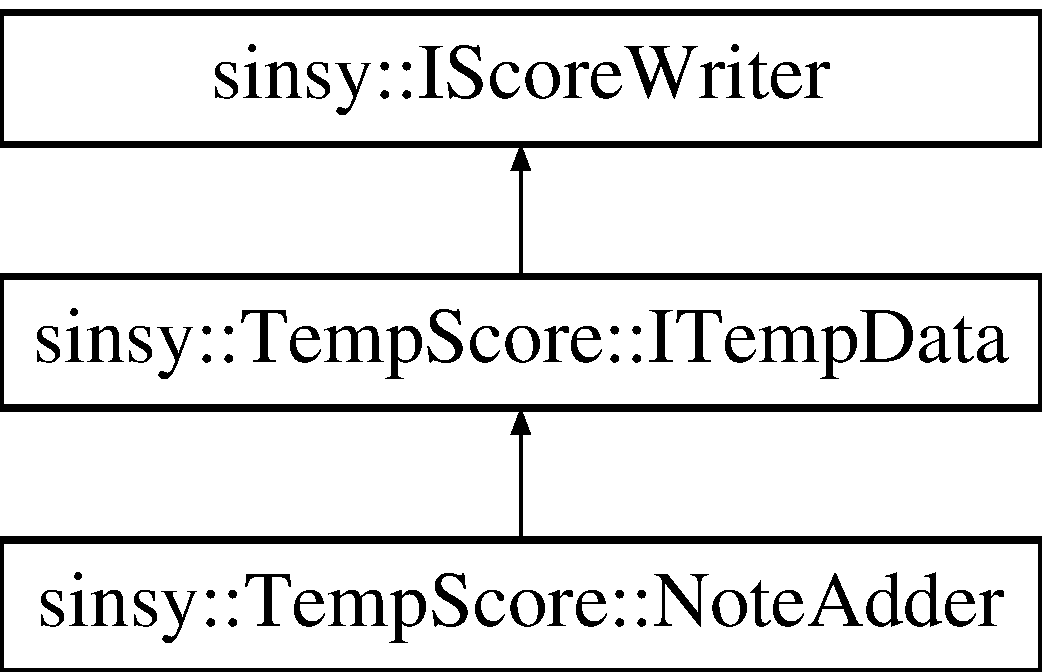
\includegraphics[height=3.000000cm]{classsinsy_1_1TempScore_1_1NoteAdder}
\end{center}
\end{figure}
\subsection*{\-Public \-Member \-Functions}
\begin{DoxyCompactItemize}
\item 
\hypertarget{classsinsy_1_1TempScore_1_1NoteAdder_add45c4f6ed26a9f2dbd924239ba2f185}{\hyperlink{classsinsy_1_1TempScore_1_1NoteAdder_add45c4f6ed26a9f2dbd924239ba2f185}{\-Note\-Adder} (const \hyperlink{classsinsy_1_1Note}{\-Note} \&n)}\label{classsinsy_1_1TempScore_1_1NoteAdder_add45c4f6ed26a9f2dbd924239ba2f185}

\begin{DoxyCompactList}\small\item\em constructor \end{DoxyCompactList}\item 
\hypertarget{classsinsy_1_1TempScore_1_1NoteAdder_a3820c55c959b1a780b4b29f5d141e316}{virtual \hyperlink{classsinsy_1_1TempScore_1_1NoteAdder_a3820c55c959b1a780b4b29f5d141e316}{$\sim$\-Note\-Adder} ()}\label{classsinsy_1_1TempScore_1_1NoteAdder_a3820c55c959b1a780b4b29f5d141e316}

\begin{DoxyCompactList}\small\item\em destructor \end{DoxyCompactList}\item 
virtual void \hyperlink{classsinsy_1_1TempScore_1_1NoteAdder_ab2a04d2b0707df96150ea24ea0e5f143}{write} (\hyperlink{classsinsy_1_1IScoreWritable}{\-I\-Score\-Writable} \&sm) const 
\begin{DoxyCompactList}\small\item\em wtrite \end{DoxyCompactList}\item 
\hypertarget{classsinsy_1_1TempScore_1_1NoteAdder_a8b2f9dbca1733f47d4a184b94933cf38}{const \hyperlink{classsinsy_1_1Note}{\-Note} \& \hyperlink{classsinsy_1_1TempScore_1_1NoteAdder_a8b2f9dbca1733f47d4a184b94933cf38}{get\-Note} () const }\label{classsinsy_1_1TempScore_1_1NoteAdder_a8b2f9dbca1733f47d4a184b94933cf38}

\begin{DoxyCompactList}\small\item\em get note \end{DoxyCompactList}\item 
\hypertarget{classsinsy_1_1TempScore_1_1NoteAdder_af268bca914497861f79ac20026a12b50}{\hyperlink{classsinsy_1_1Note}{\-Note} \& \hyperlink{classsinsy_1_1TempScore_1_1NoteAdder_af268bca914497861f79ac20026a12b50}{get\-Note} ()}\label{classsinsy_1_1TempScore_1_1NoteAdder_af268bca914497861f79ac20026a12b50}

\begin{DoxyCompactList}\small\item\em get note \end{DoxyCompactList}\end{DoxyCompactItemize}


\subsection{\-Member \-Function \-Documentation}
\hypertarget{classsinsy_1_1TempScore_1_1NoteAdder_ab2a04d2b0707df96150ea24ea0e5f143}{\index{sinsy\-::\-Temp\-Score\-::\-Note\-Adder@{sinsy\-::\-Temp\-Score\-::\-Note\-Adder}!write@{write}}
\index{write@{write}!sinsy::TempScore::NoteAdder@{sinsy\-::\-Temp\-Score\-::\-Note\-Adder}}
\subsubsection[{write}]{\setlength{\rightskip}{0pt plus 5cm}void {\bf \-Temp\-Score\-::\-Note\-Adder\-::write} (
\begin{DoxyParamCaption}
\item[{{\bf \-I\-Score\-Writable} \&}]{sm}
\end{DoxyParamCaption}
) const\hspace{0.3cm}{\ttfamily  \mbox{[}virtual\mbox{]}}}}\label{classsinsy_1_1TempScore_1_1NoteAdder_ab2a04d2b0707df96150ea24ea0e5f143}


wtrite 

write 

\-Implements \hyperlink{classsinsy_1_1TempScore_1_1ITempData_ab6d83a865088b42b62dc5a0a82e47fa5}{sinsy\-::\-Temp\-Score\-::\-I\-Temp\-Data}.



\-The documentation for this class was generated from the following files\-:\begin{DoxyCompactItemize}
\item 
lib/temporary/\-Temp\-Score.\-h\item 
lib/temporary/\-Temp\-Score.\-cpp\end{DoxyCompactItemize}

\hypertarget{classsinsy_1_1NoteGroup}{\section{sinsy\-:\-:\-Note\-Group \-Class \-Reference}
\label{classsinsy_1_1NoteGroup}\index{sinsy\-::\-Note\-Group@{sinsy\-::\-Note\-Group}}
}
\subsection*{\-Public \-Member \-Functions}
\begin{DoxyCompactItemize}
\item 
\hypertarget{classsinsy_1_1NoteGroup_ac87afe50423a143748094a2a8231fa4c}{\hyperlink{classsinsy_1_1NoteGroup_ac87afe50423a143748094a2a8231fa4c}{\-Note\-Group} ()}\label{classsinsy_1_1NoteGroup_ac87afe50423a143748094a2a8231fa4c}

\begin{DoxyCompactList}\small\item\em constructor \end{DoxyCompactList}\item 
\hypertarget{classsinsy_1_1NoteGroup_aeb30350c0cb9c25fa4ddc5e0a731a6da}{virtual \hyperlink{classsinsy_1_1NoteGroup_aeb30350c0cb9c25fa4ddc5e0a731a6da}{$\sim$\-Note\-Group} ()}\label{classsinsy_1_1NoteGroup_aeb30350c0cb9c25fa4ddc5e0a731a6da}

\begin{DoxyCompactList}\small\item\em destructor \end{DoxyCompactList}\item 
\hypertarget{classsinsy_1_1NoteGroup_a26f59e76efd9016e15bd17d5c83dd6ec}{void \hyperlink{classsinsy_1_1NoteGroup_a26f59e76efd9016e15bd17d5c83dd6ec}{add\-Position} (const \hyperlink{classsinsy_1_1LabelPosition}{\-Label\-Position} \&p)}\label{classsinsy_1_1NoteGroup_a26f59e76efd9016e15bd17d5c83dd6ec}

\begin{DoxyCompactList}\small\item\em add position \end{DoxyCompactList}\item 
\hypertarget{classsinsy_1_1NoteGroup_ad85c183b51866413aec77a5f8cbdd0f0}{const \hyperlink{classsinsy_1_1LabelPosition}{\-Label\-Position} \& \hyperlink{classsinsy_1_1NoteGroup_ad85c183b51866413aec77a5f8cbdd0f0}{get\-Position} () const }\label{classsinsy_1_1NoteGroup_ad85c183b51866413aec77a5f8cbdd0f0}

\begin{DoxyCompactList}\small\item\em get position \end{DoxyCompactList}\item 
\hypertarget{classsinsy_1_1NoteGroup_a9e78ddbac0ff1fd8cadf5c947cdba98c}{void \hyperlink{classsinsy_1_1NoteGroup_a9e78ddbac0ff1fd8cadf5c947cdba98c}{add\-Syllable\-Num} (size\-\_\-t n)}\label{classsinsy_1_1NoteGroup_a9e78ddbac0ff1fd8cadf5c947cdba98c}

\begin{DoxyCompactList}\small\item\em add number of syllables \end{DoxyCompactList}\item 
\hypertarget{classsinsy_1_1NoteGroup_a839d4263d13d7afeb23dca7d5c748b59}{size\-\_\-t \hyperlink{classsinsy_1_1NoteGroup_a839d4263d13d7afeb23dca7d5c748b59}{get\-Syllable\-Num} () const }\label{classsinsy_1_1NoteGroup_a839d4263d13d7afeb23dca7d5c748b59}

\begin{DoxyCompactList}\small\item\em get number of syllables \end{DoxyCompactList}\end{DoxyCompactItemize}


\-The documentation for this class was generated from the following files\-:\begin{DoxyCompactItemize}
\item 
lib/label/\-Note\-Group.\-h\item 
lib/label/\-Note\-Group.\-cpp\end{DoxyCompactItemize}

\hypertarget{classsinsy_1_1NoteLabeler}{\section{sinsy\-:\-:\-Note\-Labeler \-Class \-Reference}
\label{classsinsy_1_1NoteLabeler}\index{sinsy\-::\-Note\-Labeler@{sinsy\-::\-Note\-Labeler}}
}
\-Inheritance diagram for sinsy\-:\-:\-Note\-Labeler\-:\begin{figure}[H]
\begin{center}
\leavevmode
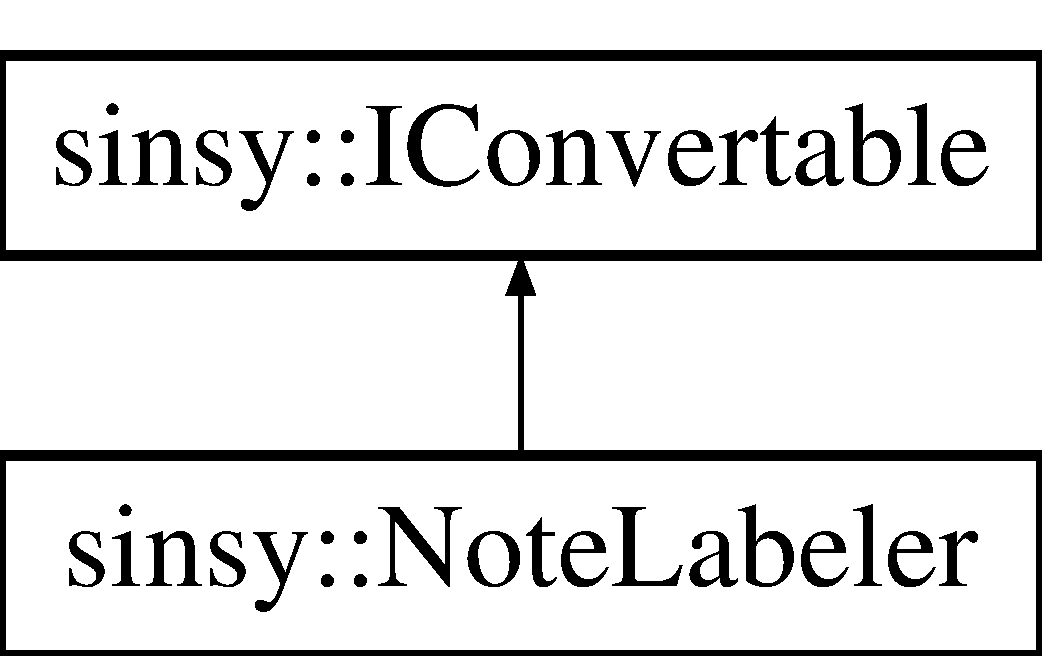
\includegraphics[height=2.000000cm]{classsinsy_1_1NoteLabeler}
\end{center}
\end{figure}
\subsection*{\-Classes}
\begin{DoxyCompactItemize}
\item 
class {\bfseries \-Note\-Data}
\item 
class {\bfseries \-Position\-Adder}
\end{DoxyCompactItemize}
\subsection*{\-Public \-Types}
\begin{DoxyCompactItemize}
\item 
\hypertarget{classsinsy_1_1NoteLabeler_a3cac0931abc74e5d2af1321739c66530}{typedef std\-::vector\*
$<$ \hyperlink{classsinsy_1_1SyllableLabeler}{\-Syllable\-Labeler} $\ast$ $>$ {\bfseries \-List}}\label{classsinsy_1_1NoteLabeler_a3cac0931abc74e5d2af1321739c66530}

\end{DoxyCompactItemize}
\subsection*{\-Public \-Member \-Functions}
\begin{DoxyCompactItemize}
\item 
\hyperlink{classsinsy_1_1NoteLabeler_a657bab991e0cdd62069a5f69aa12d6ca}{\-Note\-Labeler} (const \hyperlink{classsinsy_1_1Beat}{\-Beat} \&b, const \hyperlink{classsinsy_1_1Dynamics}{\-Dynamics} \&d, const \hyperlink{classsinsy_1_1Key}{\-Key} \&k)
\begin{DoxyCompactList}\small\item\em constructor \end{DoxyCompactList}\item 
\hypertarget{classsinsy_1_1NoteLabeler_aa3e344f5248b5e996fa945105e936a5e}{virtual \hyperlink{classsinsy_1_1NoteLabeler_aa3e344f5248b5e996fa945105e936a5e}{$\sim$\-Note\-Labeler} ()}\label{classsinsy_1_1NoteLabeler_aa3e344f5248b5e996fa945105e936a5e}

\begin{DoxyCompactList}\small\item\em destructor \end{DoxyCompactList}\item 
\hypertarget{classsinsy_1_1NoteLabeler_aef26082ba5e3ae1547922993f0c03214}{virtual bool \hyperlink{classsinsy_1_1NoteLabeler_aef26082ba5e3ae1547922993f0c03214}{is\-Rest} () const }\label{classsinsy_1_1NoteLabeler_aef26082ba5e3ae1547922993f0c03214}

\begin{DoxyCompactList}\small\item\em is rest or not \end{DoxyCompactList}\item 
\hypertarget{classsinsy_1_1NoteLabeler_aa237e645eec582031e05e873e98d510e}{virtual bool \hyperlink{classsinsy_1_1NoteLabeler_aa237e645eec582031e05e873e98d510e}{is\-Converted} () const }\label{classsinsy_1_1NoteLabeler_aa237e645eec582031e05e873e98d510e}

\begin{DoxyCompactList}\small\item\em already converted or not \end{DoxyCompactList}\item 
\hypertarget{classsinsy_1_1NoteLabeler_aa30afe19db901d524759dca56e91b2aa}{virtual std\-::string \hyperlink{classsinsy_1_1NoteLabeler_aa30afe19db901d524759dca56e91b2aa}{get\-Lyric} () const }\label{classsinsy_1_1NoteLabeler_aa30afe19db901d524759dca56e91b2aa}

\begin{DoxyCompactList}\small\item\em get lyric \end{DoxyCompactList}\item 
\hypertarget{classsinsy_1_1NoteLabeler_a4aa0089013e5598ef7e517ffcef63dea}{virtual \hyperlink{classsinsy_1_1Syllabic}{\-Syllabic} \hyperlink{classsinsy_1_1NoteLabeler_a4aa0089013e5598ef7e517ffcef63dea}{get\-Syllabic} () const }\label{classsinsy_1_1NoteLabeler_a4aa0089013e5598ef7e517ffcef63dea}

\begin{DoxyCompactList}\small\item\em get syllabic \end{DoxyCompactList}\item 
\hypertarget{classsinsy_1_1NoteLabeler_ab27386272cbbee6f9b546dcbf3555e7e}{size\-\_\-t \hyperlink{classsinsy_1_1NoteLabeler_ab27386272cbbee6f9b546dcbf3555e7e}{get\-Duration} () const }\label{classsinsy_1_1NoteLabeler_ab27386272cbbee6f9b546dcbf3555e7e}

\begin{DoxyCompactList}\small\item\em get duration \end{DoxyCompactList}\item 
virtual void \hyperlink{classsinsy_1_1NoteLabeler_a5be5f059a3b710eb0ec054d508d63e1a}{add\-Info} (const std\-::vector$<$ \hyperlink{classsinsy_1_1PhonemeInfo}{\-Phoneme\-Info} $>$ \&phonemes, const std\-::string \&language, const std\-::string \&info)
\begin{DoxyCompactList}\small\item\em add information \end{DoxyCompactList}\item 
virtual void \hyperlink{classsinsy_1_1NoteLabeler_afce8f71c437e03b1acb894a5335cbe31}{set\-Label} (\hyperlink{classsinsy_1_1INoteLabel}{\-I\-Note\-Label} \&label) const 
\begin{DoxyCompactList}\small\item\em set label \end{DoxyCompactList}\item 
void \hyperlink{classsinsy_1_1NoteLabeler_a66723aa4d1f9f4327752b9ebb2ce0061}{add\-Note} (const \hyperlink{classsinsy_1_1Note}{\-Note} \&note, double tempo)
\begin{DoxyCompactList}\small\item\em add note \end{DoxyCompactList}\item 
\hypertarget{classsinsy_1_1NoteLabeler_a39daa254597bd51f42c20002f6c47d84}{const \hyperlink{classsinsy_1_1Beat}{\-Beat} \& \hyperlink{classsinsy_1_1NoteLabeler_a39daa254597bd51f42c20002f6c47d84}{get\-Beat} () const }\label{classsinsy_1_1NoteLabeler_a39daa254597bd51f42c20002f6c47d84}

\begin{DoxyCompactList}\small\item\em get beat \end{DoxyCompactList}\item 
\hypertarget{classsinsy_1_1NoteLabeler_aeb8d197f49f778c75147b2556490bd55}{const \hyperlink{classsinsy_1_1Dynamics}{\-Dynamics} \& \hyperlink{classsinsy_1_1NoteLabeler_aeb8d197f49f778c75147b2556490bd55}{get\-Dynamics} () const }\label{classsinsy_1_1NoteLabeler_aeb8d197f49f778c75147b2556490bd55}

\begin{DoxyCompactList}\small\item\em get dynamics \end{DoxyCompactList}\item 
\hypertarget{classsinsy_1_1NoteLabeler_a334deeb6e7d6a68b92cc8eba660d722d}{const \hyperlink{classsinsy_1_1Key}{\-Key} \& \hyperlink{classsinsy_1_1NoteLabeler_a334deeb6e7d6a68b92cc8eba660d722d}{get\-Key} () const }\label{classsinsy_1_1NoteLabeler_a334deeb6e7d6a68b92cc8eba660d722d}

\begin{DoxyCompactList}\small\item\em get key \end{DoxyCompactList}\item 
\hypertarget{classsinsy_1_1NoteLabeler_a32b7b95829e4dcd5a5ac3b12e54c0b1a}{void \hyperlink{classsinsy_1_1NoteLabeler_a32b7b95829e4dcd5a5ac3b12e54c0b1a}{set\-Measure} (\hyperlink{classsinsy_1_1LabelMeasure}{\-Label\-Measure} $\ast$m)}\label{classsinsy_1_1NoteLabeler_a32b7b95829e4dcd5a5ac3b12e54c0b1a}

\begin{DoxyCompactList}\small\item\em set measure \end{DoxyCompactList}\item 
\hypertarget{classsinsy_1_1NoteLabeler_a839e0a699b31045175072ee57b85f221}{void \hyperlink{classsinsy_1_1NoteLabeler_a839e0a699b31045175072ee57b85f221}{set\-Phrase} (\hyperlink{classsinsy_1_1NoteGroup}{\-Note\-Group} $\ast$ng)}\label{classsinsy_1_1NoteLabeler_a839e0a699b31045175072ee57b85f221}

\begin{DoxyCompactList}\small\item\em set phrase \end{DoxyCompactList}\item 
\hypertarget{classsinsy_1_1NoteLabeler_a4e1024d0718e90a096488809973ee506}{void \hyperlink{classsinsy_1_1NoteLabeler_a4e1024d0718e90a096488809973ee506}{set\-Crescendo} (\hyperlink{classsinsy_1_1NoteGroup}{\-Note\-Group} $\ast$ng)}\label{classsinsy_1_1NoteLabeler_a4e1024d0718e90a096488809973ee506}

\begin{DoxyCompactList}\small\item\em set crescendo \end{DoxyCompactList}\item 
\hypertarget{classsinsy_1_1NoteLabeler_aa65646ae98b670691fb9fedbb113b8ae}{void \hyperlink{classsinsy_1_1NoteLabeler_aa65646ae98b670691fb9fedbb113b8ae}{set\-Diminuendo} (\hyperlink{classsinsy_1_1NoteGroup}{\-Note\-Group} $\ast$ng)}\label{classsinsy_1_1NoteLabeler_aa65646ae98b670691fb9fedbb113b8ae}

\begin{DoxyCompactList}\small\item\em set diminuendo \end{DoxyCompactList}\item 
void \hyperlink{classsinsy_1_1NoteLabeler_a150254899347367acf8ca1120d72e022}{set\-Prev\-Phrase} (const \hyperlink{classsinsy_1_1NoteGroup}{\-Note\-Group} $\ast$ng)
\begin{DoxyCompactList}\small\item\em set prev phrase \end{DoxyCompactList}\item 
\hypertarget{classsinsy_1_1NoteLabeler_a725c30d75ab6605dc86431e76d37c4fa}{void \hyperlink{classsinsy_1_1NoteLabeler_a725c30d75ab6605dc86431e76d37c4fa}{set\-Next\-Phrase} (const \hyperlink{classsinsy_1_1NoteGroup}{\-Note\-Group} $\ast$ng)}\label{classsinsy_1_1NoteLabeler_a725c30d75ab6605dc86431e76d37c4fa}

\begin{DoxyCompactList}\small\item\em set next phrase \end{DoxyCompactList}\item 
\hypertarget{classsinsy_1_1NoteLabeler_a60b5e5ecab863576ae53b5eda1031b8a}{const \hyperlink{classsinsy_1_1NoteGroup}{\-Note\-Group} $\ast$ \hyperlink{classsinsy_1_1NoteLabeler_a60b5e5ecab863576ae53b5eda1031b8a}{get\-Phrase} () const }\label{classsinsy_1_1NoteLabeler_a60b5e5ecab863576ae53b5eda1031b8a}

\begin{DoxyCompactList}\small\item\em get phrase \end{DoxyCompactList}\item 
\hypertarget{classsinsy_1_1NoteLabeler_a6f822ab8d3a694b9a4a255b67f37045c}{\hyperlink{classsinsy_1_1Pitch}{\-Pitch} \hyperlink{classsinsy_1_1NoteLabeler_a6f822ab8d3a694b9a4a255b67f37045c}{get\-Pitch} () const }\label{classsinsy_1_1NoteLabeler_a6f822ab8d3a694b9a4a255b67f37045c}

\begin{DoxyCompactList}\small\item\em get pitch \end{DoxyCompactList}\item 
\hypertarget{classsinsy_1_1NoteLabeler_a6ef98ccd80d5fda798c412c65cb18b5b}{void \hyperlink{classsinsy_1_1NoteLabeler_a6ef98ccd80d5fda798c412c65cb18b5b}{set\-Positions} ()}\label{classsinsy_1_1NoteLabeler_a6ef98ccd80d5fda798c412c65cb18b5b}

\begin{DoxyCompactList}\small\item\em set positions \end{DoxyCompactList}\item 
\hypertarget{classsinsy_1_1NoteLabeler_af656e318faf7d9afc078ae76dfd10445}{bool \hyperlink{classsinsy_1_1NoteLabeler_af656e318faf7d9afc078ae76dfd10445}{is\-Slur\-Start} () const }\label{classsinsy_1_1NoteLabeler_af656e318faf7d9afc078ae76dfd10445}

\begin{DoxyCompactList}\small\item\em is slur start or not \end{DoxyCompactList}\item 
\hypertarget{classsinsy_1_1NoteLabeler_a9be513c0e60fb53ff13c41fae804183c}{bool \hyperlink{classsinsy_1_1NoteLabeler_a9be513c0e60fb53ff13c41fae804183c}{is\-Slur\-Stop} () const }\label{classsinsy_1_1NoteLabeler_a9be513c0e60fb53ff13c41fae804183c}

\begin{DoxyCompactList}\small\item\em is slur stop or not \end{DoxyCompactList}\item 
\hypertarget{classsinsy_1_1NoteLabeler_a3ff27da70679310dd019fae2bc31eb44}{void \hyperlink{classsinsy_1_1NoteLabeler_a3ff27da70679310dd019fae2bc31eb44}{set\-In\-Slur\-From\-Prev} (bool b)}\label{classsinsy_1_1NoteLabeler_a3ff27da70679310dd019fae2bc31eb44}

\begin{DoxyCompactList}\small\item\em set if this note is in slur from previous note or not \end{DoxyCompactList}\item 
\hypertarget{classsinsy_1_1NoteLabeler_a0b132a68721cd55597515f050eb39596}{void \hyperlink{classsinsy_1_1NoteLabeler_a0b132a68721cd55597515f050eb39596}{set\-In\-Slur\-To\-Next} (bool b)}\label{classsinsy_1_1NoteLabeler_a0b132a68721cd55597515f050eb39596}

\begin{DoxyCompactList}\small\item\em set if this note is in slur to next note or not \end{DoxyCompactList}\item 
\hypertarget{classsinsy_1_1NoteLabeler_a4cfaaf6fb7f0c43dc27e8583456c89a6}{void \hyperlink{classsinsy_1_1NoteLabeler_a4cfaaf6fb7f0c43dc27e8583456c89a6}{set\-Prev\-Pitch} (const \hyperlink{classsinsy_1_1Pitch}{\-Pitch} \&p)}\label{classsinsy_1_1NoteLabeler_a4cfaaf6fb7f0c43dc27e8583456c89a6}

\begin{DoxyCompactList}\small\item\em set previous pitch \end{DoxyCompactList}\item 
\hypertarget{classsinsy_1_1NoteLabeler_aecd9c1c38124746b15e5cf9ed158b146}{void \hyperlink{classsinsy_1_1NoteLabeler_aecd9c1c38124746b15e5cf9ed158b146}{set\-Next\-Pitch} (const \hyperlink{classsinsy_1_1Pitch}{\-Pitch} \&p)}\label{classsinsy_1_1NoteLabeler_aecd9c1c38124746b15e5cf9ed158b146}

\begin{DoxyCompactList}\small\item\em set next pitch \end{DoxyCompactList}\item 
\hypertarget{classsinsy_1_1NoteLabeler_aeeb9701786f11b28567af19fde462883}{\hyperlink{classsinsy_1_1LabelPosition}{\-Label\-Position} \hyperlink{classsinsy_1_1NoteLabeler_aeeb9701786f11b28567af19fde462883}{get\-Length} () const }\label{classsinsy_1_1NoteLabeler_aeeb9701786f11b28567af19fde462883}

\begin{DoxyCompactList}\small\item\em get length \end{DoxyCompactList}\item 
\hypertarget{classsinsy_1_1NoteLabeler_a71a9479c90f11c463f7c0b0bf7791171}{void \hyperlink{classsinsy_1_1NoteLabeler_a71a9479c90f11c463f7c0b0bf7791171}{set\-Next\-Accent\-Position} (const \hyperlink{classsinsy_1_1LabelPosition}{\-Label\-Position} \&p)}\label{classsinsy_1_1NoteLabeler_a71a9479c90f11c463f7c0b0bf7791171}

\begin{DoxyCompactList}\small\item\em set next accent position \end{DoxyCompactList}\item 
\hypertarget{classsinsy_1_1NoteLabeler_af1c1addbc22436b34a6745516575df6c}{void \hyperlink{classsinsy_1_1NoteLabeler_af1c1addbc22436b34a6745516575df6c}{set\-Prev\-Accent\-Position} (const \hyperlink{classsinsy_1_1LabelPosition}{\-Label\-Position} \&p)}\label{classsinsy_1_1NoteLabeler_af1c1addbc22436b34a6745516575df6c}

\begin{DoxyCompactList}\small\item\em set previous accent position \end{DoxyCompactList}\item 
\hypertarget{classsinsy_1_1NoteLabeler_a9440199882ee72394e65b909a850eae6}{void \hyperlink{classsinsy_1_1NoteLabeler_a9440199882ee72394e65b909a850eae6}{set\-Next\-Staccato\-Position} (const \hyperlink{classsinsy_1_1LabelPosition}{\-Label\-Position} \&p)}\label{classsinsy_1_1NoteLabeler_a9440199882ee72394e65b909a850eae6}

\begin{DoxyCompactList}\small\item\em set next staccato position \end{DoxyCompactList}\item 
\hypertarget{classsinsy_1_1NoteLabeler_abb3aa7af6ac0a0dc232bee355f754f45}{void \hyperlink{classsinsy_1_1NoteLabeler_abb3aa7af6ac0a0dc232bee355f754f45}{set\-Prev\-Staccato\-Position} (const \hyperlink{classsinsy_1_1LabelPosition}{\-Label\-Position} \&p)}\label{classsinsy_1_1NoteLabeler_abb3aa7af6ac0a0dc232bee355f754f45}

\begin{DoxyCompactList}\small\item\em set previous staccato position \end{DoxyCompactList}\item 
\hypertarget{classsinsy_1_1NoteLabeler_aa86d0a233d1668cefba30448ae22e633}{size\-\_\-t \hyperlink{classsinsy_1_1NoteLabeler_aa86d0a233d1668cefba30448ae22e633}{get\-Syllable\-Num} () const }\label{classsinsy_1_1NoteLabeler_aa86d0a233d1668cefba30448ae22e633}

\begin{DoxyCompactList}\small\item\em get number of syllables \end{DoxyCompactList}\item 
\hypertarget{classsinsy_1_1NoteLabeler_a2bbb700b2b7821989fc483e73956026d}{bool \hyperlink{classsinsy_1_1NoteLabeler_a2bbb700b2b7821989fc483e73956026d}{has\-Accent} () const }\label{classsinsy_1_1NoteLabeler_a2bbb700b2b7821989fc483e73956026d}

\begin{DoxyCompactList}\small\item\em has accent or not \end{DoxyCompactList}\item 
\hypertarget{classsinsy_1_1NoteLabeler_aeceb66873cede3f7cea5f586238df450}{bool \hyperlink{classsinsy_1_1NoteLabeler_aeceb66873cede3f7cea5f586238df450}{has\-Staccato} () const }\label{classsinsy_1_1NoteLabeler_aeceb66873cede3f7cea5f586238df450}

\begin{DoxyCompactList}\small\item\em has staccato or not \end{DoxyCompactList}\item 
bool \hyperlink{classsinsy_1_1NoteLabeler_a967b7e5375d754eed4df1a123b06ac91}{has\-Breath\-To\-Next} () const 
\begin{DoxyCompactList}\small\item\em if this note has breath between this and next node, return true. \end{DoxyCompactList}\item 
\hypertarget{classsinsy_1_1NoteLabeler_a8582f7667aec7650595d3e040f47b946}{void \hyperlink{classsinsy_1_1NoteLabeler_a8582f7667aec7650595d3e040f47b946}{set\-Prev\-Note} (const \hyperlink{classsinsy_1_1NoteLabeler}{\-Note\-Labeler} $\ast$prev)}\label{classsinsy_1_1NoteLabeler_a8582f7667aec7650595d3e040f47b946}

\begin{DoxyCompactList}\small\item\em set previous note (null -\/$>$ this is the head note) \end{DoxyCompactList}\item 
\hypertarget{classsinsy_1_1NoteLabeler_a4dbe152f588f27032b014279fe6fc91b}{void \hyperlink{classsinsy_1_1NoteLabeler_a4dbe152f588f27032b014279fe6fc91b}{set\-Next\-Note} (const \hyperlink{classsinsy_1_1NoteLabeler}{\-Note\-Labeler} $\ast$next)}\label{classsinsy_1_1NoteLabeler_a4dbe152f588f27032b014279fe6fc91b}

\begin{DoxyCompactList}\small\item\em set next note (null -\/$>$ this is the tail note) \end{DoxyCompactList}\item 
const \hyperlink{classsinsy_1_1LabelPosition}{\-Label\-Position} \& \hyperlink{classsinsy_1_1NoteLabeler_af3687d74b7cff50bd6797d5a77e54163}{get\-Measure\-Idx} () const 
\begin{DoxyCompactList}\small\item\em ... \end{DoxyCompactList}\item 
void \hyperlink{classsinsy_1_1NoteLabeler_acafb879727f06489887e3177ce15f8a3}{move\-To} (\hyperlink{classsinsy_1_1NoteLabeler}{\-Note\-Labeler} \&, size\-\_\-t=0)
\begin{DoxyCompactList}\small\item\em ... \end{DoxyCompactList}\item 
\hypertarget{classsinsy_1_1NoteLabeler_ad2d131247f0b2bfa19e4bbc9ab323006}{void \hyperlink{classsinsy_1_1NoteLabeler_ad2d131247f0b2bfa19e4bbc9ab323006}{set\-Breath\-Phoneme} ()}\label{classsinsy_1_1NoteLabeler_ad2d131247f0b2bfa19e4bbc9ab323006}

\begin{DoxyCompactList}\small\item\em set breath phoneme to the tail of the last syllable \end{DoxyCompactList}\item 
\-List\-::const\-\_\-iterator \hyperlink{classsinsy_1_1NoteLabeler_ae585d35c99fe782630e435d0dc81f4a5}{child\-Begin} () const 
\begin{DoxyCompactList}\small\item\em get begin iteration \end{DoxyCompactList}\item 
\-List\-::const\-\_\-iterator \hyperlink{classsinsy_1_1NoteLabeler_ad321546de9365caf2f46d1d5cf255996}{child\-End} () const 
\begin{DoxyCompactList}\small\item\em get end iteration \end{DoxyCompactList}\end{DoxyCompactItemize}


\subsection{\-Constructor \& \-Destructor \-Documentation}
\hypertarget{classsinsy_1_1NoteLabeler_a657bab991e0cdd62069a5f69aa12d6ca}{\index{sinsy\-::\-Note\-Labeler@{sinsy\-::\-Note\-Labeler}!\-Note\-Labeler@{\-Note\-Labeler}}
\index{\-Note\-Labeler@{\-Note\-Labeler}!sinsy::NoteLabeler@{sinsy\-::\-Note\-Labeler}}
\subsubsection[{\-Note\-Labeler}]{\setlength{\rightskip}{0pt plus 5cm}{\bf \-Note\-Labeler\-::\-Note\-Labeler} (
\begin{DoxyParamCaption}
\item[{const {\bf \-Beat} \&}]{b, }
\item[{const {\bf \-Dynamics} \&}]{d, }
\item[{const {\bf \-Key} \&}]{k}
\end{DoxyParamCaption}
)}}\label{classsinsy_1_1NoteLabeler_a657bab991e0cdd62069a5f69aa12d6ca}


constructor 

constructor


\begin{DoxyParams}{\-Parameters}
{\em b} & beat \\
\hline
{\em d} & dynamics \\
\hline
{\em k} & key \\
\hline
\end{DoxyParams}


\subsection{\-Member \-Function \-Documentation}
\hypertarget{classsinsy_1_1NoteLabeler_a5be5f059a3b710eb0ec054d508d63e1a}{\index{sinsy\-::\-Note\-Labeler@{sinsy\-::\-Note\-Labeler}!add\-Info@{add\-Info}}
\index{add\-Info@{add\-Info}!sinsy::NoteLabeler@{sinsy\-::\-Note\-Labeler}}
\subsubsection[{add\-Info}]{\setlength{\rightskip}{0pt plus 5cm}void {\bf \-Note\-Labeler\-::add\-Info} (
\begin{DoxyParamCaption}
\item[{const std\-::vector$<$ {\bf \-Phoneme\-Info} $>$ \&}]{phonemes, }
\item[{const std\-::string \&}]{language, }
\item[{const std\-::string \&}]{info}
\end{DoxyParamCaption}
)\hspace{0.3cm}{\ttfamily  \mbox{[}virtual\mbox{]}}}}\label{classsinsy_1_1NoteLabeler_a5be5f059a3b710eb0ec054d508d63e1a}


add information 

add information


\begin{DoxyParams}{\-Parameters}
{\em phonemes} & phoneme list \\
\hline
{\em language} & language \\
\hline
{\em info} & language dependent information \\
\hline
\end{DoxyParams}


\-Implements \hyperlink{classsinsy_1_1IConvertable_ae0326517f226fc7f569b5886084d6135}{sinsy\-::\-I\-Convertable}.

\hypertarget{classsinsy_1_1NoteLabeler_a66723aa4d1f9f4327752b9ebb2ce0061}{\index{sinsy\-::\-Note\-Labeler@{sinsy\-::\-Note\-Labeler}!add\-Note@{add\-Note}}
\index{add\-Note@{add\-Note}!sinsy::NoteLabeler@{sinsy\-::\-Note\-Labeler}}
\subsubsection[{add\-Note}]{\setlength{\rightskip}{0pt plus 5cm}void {\bf \-Note\-Labeler\-::add\-Note} (
\begin{DoxyParamCaption}
\item[{const {\bf \-Note} \&}]{note, }
\item[{double}]{tempo}
\end{DoxyParamCaption}
)}}\label{classsinsy_1_1NoteLabeler_a66723aa4d1f9f4327752b9ebb2ce0061}


add note 

add note


\begin{DoxyParams}{\-Parameters}
{\em note} & note \\
\hline
{\em tempo} & tempo \\
\hline
\end{DoxyParams}
\hypertarget{classsinsy_1_1NoteLabeler_ae585d35c99fe782630e435d0dc81f4a5}{\index{sinsy\-::\-Note\-Labeler@{sinsy\-::\-Note\-Labeler}!child\-Begin@{child\-Begin}}
\index{child\-Begin@{child\-Begin}!sinsy::NoteLabeler@{sinsy\-::\-Note\-Labeler}}
\subsubsection[{child\-Begin}]{\setlength{\rightskip}{0pt plus 5cm}\-Note\-Labeler\-::\-List\-::const\-\_\-iterator {\bf \-Note\-Labeler\-::child\-Begin} (
\begin{DoxyParamCaption}
{}
\end{DoxyParamCaption}
) const}}\label{classsinsy_1_1NoteLabeler_ae585d35c99fe782630e435d0dc81f4a5}


get begin iteration 

get begin iterator of syllables \hypertarget{classsinsy_1_1NoteLabeler_ad321546de9365caf2f46d1d5cf255996}{\index{sinsy\-::\-Note\-Labeler@{sinsy\-::\-Note\-Labeler}!child\-End@{child\-End}}
\index{child\-End@{child\-End}!sinsy::NoteLabeler@{sinsy\-::\-Note\-Labeler}}
\subsubsection[{child\-End}]{\setlength{\rightskip}{0pt plus 5cm}\-Note\-Labeler\-::\-List\-::const\-\_\-iterator {\bf \-Note\-Labeler\-::child\-End} (
\begin{DoxyParamCaption}
{}
\end{DoxyParamCaption}
) const}}\label{classsinsy_1_1NoteLabeler_ad321546de9365caf2f46d1d5cf255996}


get end iteration 

get end iterator of syllables \hypertarget{classsinsy_1_1NoteLabeler_af3687d74b7cff50bd6797d5a77e54163}{\index{sinsy\-::\-Note\-Labeler@{sinsy\-::\-Note\-Labeler}!get\-Measure\-Idx@{get\-Measure\-Idx}}
\index{get\-Measure\-Idx@{get\-Measure\-Idx}!sinsy::NoteLabeler@{sinsy\-::\-Note\-Labeler}}
\subsubsection[{get\-Measure\-Idx}]{\setlength{\rightskip}{0pt plus 5cm}const {\bf \-Label\-Position} \& {\bf \-Note\-Labeler\-::get\-Measure\-Idx} (
\begin{DoxyParamCaption}
{}
\end{DoxyParamCaption}
) const}}\label{classsinsy_1_1NoteLabeler_af3687d74b7cff50bd6797d5a77e54163}


... 

get measure index \hypertarget{classsinsy_1_1NoteLabeler_a967b7e5375d754eed4df1a123b06ac91}{\index{sinsy\-::\-Note\-Labeler@{sinsy\-::\-Note\-Labeler}!has\-Breath\-To\-Next@{has\-Breath\-To\-Next}}
\index{has\-Breath\-To\-Next@{has\-Breath\-To\-Next}!sinsy::NoteLabeler@{sinsy\-::\-Note\-Labeler}}
\subsubsection[{has\-Breath\-To\-Next}]{\setlength{\rightskip}{0pt plus 5cm}bool {\bf \-Note\-Labeler\-::has\-Breath\-To\-Next} (
\begin{DoxyParamCaption}
{}
\end{DoxyParamCaption}
) const}}\label{classsinsy_1_1NoteLabeler_a967b7e5375d754eed4df1a123b06ac91}


if this note has breath between this and next node, return true. 

has breath between this and next notes or not \hypertarget{classsinsy_1_1NoteLabeler_acafb879727f06489887e3177ce15f8a3}{\index{sinsy\-::\-Note\-Labeler@{sinsy\-::\-Note\-Labeler}!move\-To@{move\-To}}
\index{move\-To@{move\-To}!sinsy::NoteLabeler@{sinsy\-::\-Note\-Labeler}}
\subsubsection[{move\-To}]{\setlength{\rightskip}{0pt plus 5cm}void {\bf \-Note\-Labeler\-::move\-To} (
\begin{DoxyParamCaption}
\item[{{\bf \-Note\-Labeler} \&}]{target, }
\item[{size\-\_\-t}]{duration\-Start\-Idx = {\ttfamily 0}}
\end{DoxyParamCaption}
)}}\label{classsinsy_1_1NoteLabeler_acafb879727f06489887e3177ce15f8a3}


... 

move to target \hypertarget{classsinsy_1_1NoteLabeler_afce8f71c437e03b1acb894a5335cbe31}{\index{sinsy\-::\-Note\-Labeler@{sinsy\-::\-Note\-Labeler}!set\-Label@{set\-Label}}
\index{set\-Label@{set\-Label}!sinsy::NoteLabeler@{sinsy\-::\-Note\-Labeler}}
\subsubsection[{set\-Label}]{\setlength{\rightskip}{0pt plus 5cm}void {\bf \-Note\-Labeler\-::set\-Label} (
\begin{DoxyParamCaption}
\item[{{\bf \-I\-Note\-Label} \&}]{label}
\end{DoxyParamCaption}
) const\hspace{0.3cm}{\ttfamily  \mbox{[}virtual\mbox{]}}}}\label{classsinsy_1_1NoteLabeler_afce8f71c437e03b1acb894a5335cbe31}


set label 

set label


\begin{DoxyParams}{\-Parameters}
{\em label} & label \\
\hline
\end{DoxyParams}
\hypertarget{classsinsy_1_1NoteLabeler_a150254899347367acf8ca1120d72e022}{\index{sinsy\-::\-Note\-Labeler@{sinsy\-::\-Note\-Labeler}!set\-Prev\-Phrase@{set\-Prev\-Phrase}}
\index{set\-Prev\-Phrase@{set\-Prev\-Phrase}!sinsy::NoteLabeler@{sinsy\-::\-Note\-Labeler}}
\subsubsection[{set\-Prev\-Phrase}]{\setlength{\rightskip}{0pt plus 5cm}void {\bf \-Note\-Labeler\-::set\-Prev\-Phrase} (
\begin{DoxyParamCaption}
\item[{const {\bf \-Note\-Group} $\ast$}]{ng}
\end{DoxyParamCaption}
)}}\label{classsinsy_1_1NoteLabeler_a150254899347367acf8ca1120d72e022}


set prev phrase 

set previous phrase 

\-The documentation for this class was generated from the following files\-:\begin{DoxyCompactItemize}
\item 
lib/label/\-Note\-Labeler.\-h\item 
lib/label/\-Note\-Labeler.\-cpp\end{DoxyCompactItemize}

\hypertarget{classsinsy_1_1OutputFile}{\section{sinsy\-:\-:\-Output\-File \-Class \-Reference}
\label{classsinsy_1_1OutputFile}\index{sinsy\-::\-Output\-File@{sinsy\-::\-Output\-File}}
}
\-Inheritance diagram for sinsy\-:\-:\-Output\-File\-:\begin{figure}[H]
\begin{center}
\leavevmode
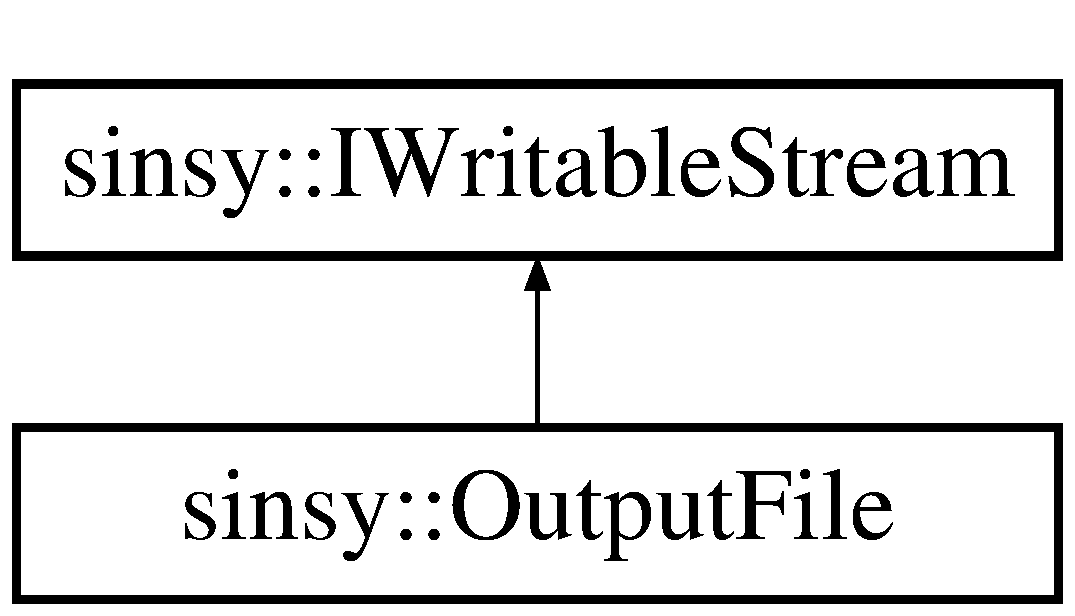
\includegraphics[height=2.000000cm]{classsinsy_1_1OutputFile}
\end{center}
\end{figure}
\subsection*{\-Public \-Member \-Functions}
\begin{DoxyCompactItemize}
\item 
\hypertarget{classsinsy_1_1OutputFile_a95bb75917bcceaef990fb39740fbb2e5}{\hyperlink{classsinsy_1_1OutputFile_a95bb75917bcceaef990fb39740fbb2e5}{\-Output\-File} ()}\label{classsinsy_1_1OutputFile_a95bb75917bcceaef990fb39740fbb2e5}

\begin{DoxyCompactList}\small\item\em constructor \end{DoxyCompactList}\item 
\hypertarget{classsinsy_1_1OutputFile_a2ecf001f9df985d47896db2e772bbb16}{\hyperlink{classsinsy_1_1OutputFile_a2ecf001f9df985d47896db2e772bbb16}{\-Output\-File} (const std\-::string \&fpath)}\label{classsinsy_1_1OutputFile_a2ecf001f9df985d47896db2e772bbb16}

\begin{DoxyCompactList}\small\item\em constructor \end{DoxyCompactList}\item 
\hypertarget{classsinsy_1_1OutputFile_ada2c24978592ca8e9dc451fe7d074b69}{virtual \hyperlink{classsinsy_1_1OutputFile_ada2c24978592ca8e9dc451fe7d074b69}{$\sim$\-Output\-File} ()}\label{classsinsy_1_1OutputFile_ada2c24978592ca8e9dc451fe7d074b69}

\begin{DoxyCompactList}\small\item\em destructor \end{DoxyCompactList}\item 
size\-\_\-t \hyperlink{classsinsy_1_1OutputFile_a50aa606271487a08ad2eb59268007f26}{write} (const void $\ast$buffer, size\-\_\-t size)  throw (\-Stream\-Exception)
\begin{DoxyCompactList}\small\item\em write to stream \end{DoxyCompactList}\item 
\hypertarget{classsinsy_1_1OutputFile_a4cd1e0efb838d18a7d62af6ce014f9bf}{void \hyperlink{classsinsy_1_1OutputFile_a4cd1e0efb838d18a7d62af6ce014f9bf}{open} (const std\-::string \&fpath)}\label{classsinsy_1_1OutputFile_a4cd1e0efb838d18a7d62af6ce014f9bf}

\begin{DoxyCompactList}\small\item\em open \end{DoxyCompactList}\item 
\hypertarget{classsinsy_1_1OutputFile_af536aa5fb243510a0f4001d2d3a001ea}{void \hyperlink{classsinsy_1_1OutputFile_af536aa5fb243510a0f4001d2d3a001ea}{close} ()}\label{classsinsy_1_1OutputFile_af536aa5fb243510a0f4001d2d3a001ea}

\begin{DoxyCompactList}\small\item\em close \end{DoxyCompactList}\item 
\hypertarget{classsinsy_1_1OutputFile_a4c19ec1bab398894e67a8eaefd5138cb}{bool \hyperlink{classsinsy_1_1OutputFile_a4c19ec1bab398894e67a8eaefd5138cb}{is\-Valid} () const }\label{classsinsy_1_1OutputFile_a4c19ec1bab398894e67a8eaefd5138cb}

\begin{DoxyCompactList}\small\item\em stream is valid or not \end{DoxyCompactList}\end{DoxyCompactItemize}


\subsection{\-Member \-Function \-Documentation}
\hypertarget{classsinsy_1_1OutputFile_a50aa606271487a08ad2eb59268007f26}{\index{sinsy\-::\-Output\-File@{sinsy\-::\-Output\-File}!write@{write}}
\index{write@{write}!sinsy::OutputFile@{sinsy\-::\-Output\-File}}
\subsubsection[{write}]{\setlength{\rightskip}{0pt plus 5cm}size\-\_\-t {\bf \-Output\-File\-::write} (
\begin{DoxyParamCaption}
\item[{const void $\ast$}]{buffer, }
\item[{size\-\_\-t}]{size}
\end{DoxyParamCaption}
)  throw ({\bf \-Stream\-Exception})\hspace{0.3cm}{\ttfamily  \mbox{[}virtual\mbox{]}}}}\label{classsinsy_1_1OutputFile_a50aa606271487a08ad2eb59268007f26}


write to stream 

write data to stream 
\begin{DoxyParams}{\-Parameters}
{\em buffer} & buffer for data that you want to write \\
\hline
{\em byte} & byte you want to write \\
\hline
\end{DoxyParams}
\begin{DoxyReturn}{\-Returns}
write bytes 
\end{DoxyReturn}


\-Implements \hyperlink{classsinsy_1_1IWritableStream_a0e7f8f7e1c41c6edd1b0d540957ba1cc}{sinsy\-::\-I\-Writable\-Stream}.



\-The documentation for this class was generated from the following files\-:\begin{DoxyCompactItemize}
\item 
lib/util/\-Output\-File.\-h\item 
lib/util/\-Output\-File.\-cpp\end{DoxyCompactItemize}

\hypertarget{classsinsy_1_1PhonemeInfo}{\section{sinsy\-:\-:\-Phoneme\-Info \-Class \-Reference}
\label{classsinsy_1_1PhonemeInfo}\index{sinsy\-::\-Phoneme\-Info@{sinsy\-::\-Phoneme\-Info}}
}
\subsection*{\-Public \-Member \-Functions}
\begin{DoxyCompactItemize}
\item 
\hypertarget{classsinsy_1_1PhonemeInfo_a617535e7cd483f0883798f0f021d9790}{\hyperlink{classsinsy_1_1PhonemeInfo_a617535e7cd483f0883798f0f021d9790}{\-Phoneme\-Info} ()}\label{classsinsy_1_1PhonemeInfo_a617535e7cd483f0883798f0f021d9790}

\begin{DoxyCompactList}\small\item\em constructor \end{DoxyCompactList}\item 
\hypertarget{classsinsy_1_1PhonemeInfo_ad5406034f30d9997184c58ff353247df}{\hyperlink{classsinsy_1_1PhonemeInfo_ad5406034f30d9997184c58ff353247df}{\-Phoneme\-Info} (const std\-::string \&type, const std\-::string \&phoneme, bool e=true, bool f=false)}\label{classsinsy_1_1PhonemeInfo_ad5406034f30d9997184c58ff353247df}

\begin{DoxyCompactList}\small\item\em constructor \end{DoxyCompactList}\item 
\hypertarget{classsinsy_1_1PhonemeInfo_a2b4622acacaf8d8ba80eb5a1d770baac}{\hyperlink{classsinsy_1_1PhonemeInfo_a2b4622acacaf8d8ba80eb5a1d770baac}{\-Phoneme\-Info} (const \hyperlink{classsinsy_1_1PhonemeInfo}{\-Phoneme\-Info} \&obj)}\label{classsinsy_1_1PhonemeInfo_a2b4622acacaf8d8ba80eb5a1d770baac}

\begin{DoxyCompactList}\small\item\em copy constructor \end{DoxyCompactList}\item 
\hypertarget{classsinsy_1_1PhonemeInfo_ae88e3093623dd8e7f59649ceb28ba8af}{virtual \hyperlink{classsinsy_1_1PhonemeInfo_ae88e3093623dd8e7f59649ceb28ba8af}{$\sim$\-Phoneme\-Info} ()}\label{classsinsy_1_1PhonemeInfo_ae88e3093623dd8e7f59649ceb28ba8af}

\begin{DoxyCompactList}\small\item\em destructor \end{DoxyCompactList}\item 
\hypertarget{classsinsy_1_1PhonemeInfo_ad1a23198e02897ab36e0bc66e652c59d}{\hyperlink{classsinsy_1_1PhonemeInfo}{\-Phoneme\-Info} \& \hyperlink{classsinsy_1_1PhonemeInfo_ad1a23198e02897ab36e0bc66e652c59d}{operator=} (const \hyperlink{classsinsy_1_1PhonemeInfo}{\-Phoneme\-Info} \&)}\label{classsinsy_1_1PhonemeInfo_ad1a23198e02897ab36e0bc66e652c59d}

\begin{DoxyCompactList}\small\item\em assignment operator \end{DoxyCompactList}\item 
\hypertarget{classsinsy_1_1PhonemeInfo_a47fc88b631936e6c69255e46153ce590}{const std\-::string \& \hyperlink{classsinsy_1_1PhonemeInfo_a47fc88b631936e6c69255e46153ce590}{get\-Type} () const }\label{classsinsy_1_1PhonemeInfo_a47fc88b631936e6c69255e46153ce590}

\begin{DoxyCompactList}\small\item\em get type \end{DoxyCompactList}\item 
\hypertarget{classsinsy_1_1PhonemeInfo_ae93f72978ddfd335b28530143014f1c5}{const std\-::string \& \hyperlink{classsinsy_1_1PhonemeInfo_ae93f72978ddfd335b28530143014f1c5}{get\-Phoneme} () const }\label{classsinsy_1_1PhonemeInfo_ae93f72978ddfd335b28530143014f1c5}

\begin{DoxyCompactList}\small\item\em get phoneme \end{DoxyCompactList}\item 
\hypertarget{classsinsy_1_1PhonemeInfo_a3bd37ae7feb6f2646f71a0cafa81722c}{bool \hyperlink{classsinsy_1_1PhonemeInfo_a3bd37ae7feb6f2646f71a0cafa81722c}{is\-Enable} () const }\label{classsinsy_1_1PhonemeInfo_a3bd37ae7feb6f2646f71a0cafa81722c}

\begin{DoxyCompactList}\small\item\em return which enable or not \end{DoxyCompactList}\item 
\hypertarget{classsinsy_1_1PhonemeInfo_a8663710459dd3f5bc6eeee71ca658d73}{bool \hyperlink{classsinsy_1_1PhonemeInfo_a8663710459dd3f5bc6eeee71ca658d73}{is\-Falsetto} () const }\label{classsinsy_1_1PhonemeInfo_a8663710459dd3f5bc6eeee71ca658d73}

\begin{DoxyCompactList}\small\item\em return which falsetto or not \end{DoxyCompactList}\end{DoxyCompactItemize}
\subsection*{\-Static \-Public \-Attributes}
\begin{DoxyCompactItemize}
\item 
\hypertarget{classsinsy_1_1PhonemeInfo_a6774418020b6be35e68b117d59a92d5a}{static const std\-::string {\bfseries \-T\-Y\-P\-E\-\_\-\-S\-I\-L\-E\-N\-T} = \char`\"{}s\char`\"{}}\label{classsinsy_1_1PhonemeInfo_a6774418020b6be35e68b117d59a92d5a}

\item 
\hypertarget{classsinsy_1_1PhonemeInfo_a6d6c06ae1b9458f8d6ea7376bda07316}{static const std\-::string {\bfseries \-T\-Y\-P\-E\-\_\-\-P\-A\-U\-S\-E} = \char`\"{}p\char`\"{}}\label{classsinsy_1_1PhonemeInfo_a6d6c06ae1b9458f8d6ea7376bda07316}

\item 
\hypertarget{classsinsy_1_1PhonemeInfo_a28436d8bf5c117d481d63ace30e6fb77}{static const std\-::string {\bfseries \-T\-Y\-P\-E\-\_\-\-V\-O\-W\-E\-L} = \char`\"{}v\char`\"{}}\label{classsinsy_1_1PhonemeInfo_a28436d8bf5c117d481d63ace30e6fb77}

\item 
\hypertarget{classsinsy_1_1PhonemeInfo_acfd4cc1a64f7902816502aa56e0b0f18}{static const std\-::string {\bfseries \-T\-Y\-P\-E\-\_\-\-C\-O\-N\-S\-O\-N\-A\-N\-T} = \char`\"{}c\char`\"{}}\label{classsinsy_1_1PhonemeInfo_acfd4cc1a64f7902816502aa56e0b0f18}

\item 
\hypertarget{classsinsy_1_1PhonemeInfo_acab80523b911adc4c76ea6d273e89b71}{static const std\-::string {\bfseries \-T\-Y\-P\-E\-\_\-\-B\-R\-E\-A\-K} = \char`\"{}b\char`\"{}}\label{classsinsy_1_1PhonemeInfo_acab80523b911adc4c76ea6d273e89b71}

\end{DoxyCompactItemize}


\-The documentation for this class was generated from the following files\-:\begin{DoxyCompactItemize}
\item 
lib/converter/\-Phoneme\-Info.\-h\item 
lib/converter/\-Phoneme\-Info.\-cpp\end{DoxyCompactItemize}

\hypertarget{classsinsy_1_1PhonemeLabeler}{\section{sinsy\-:\-:\-Phoneme\-Labeler \-Class \-Reference}
\label{classsinsy_1_1PhonemeLabeler}\index{sinsy\-::\-Phoneme\-Labeler@{sinsy\-::\-Phoneme\-Labeler}}
}
\subsection*{\-Public \-Member \-Functions}
\begin{DoxyCompactItemize}
\item 
\hypertarget{classsinsy_1_1PhonemeLabeler_a4c62e5d4d12f92b9810dc999182fcd54}{\hyperlink{classsinsy_1_1PhonemeLabeler_a4c62e5d4d12f92b9810dc999182fcd54}{\-Phoneme\-Labeler} (const \hyperlink{classsinsy_1_1PhonemeInfo}{\-Phoneme\-Info} \&)}\label{classsinsy_1_1PhonemeLabeler_a4c62e5d4d12f92b9810dc999182fcd54}

\begin{DoxyCompactList}\small\item\em constructor \end{DoxyCompactList}\item 
\hypertarget{classsinsy_1_1PhonemeLabeler_a4392240dc446f933cc9c2b07c2b7bff0}{virtual \hyperlink{classsinsy_1_1PhonemeLabeler_a4392240dc446f933cc9c2b07c2b7bff0}{$\sim$\-Phoneme\-Labeler} ()}\label{classsinsy_1_1PhonemeLabeler_a4392240dc446f933cc9c2b07c2b7bff0}

\begin{DoxyCompactList}\small\item\em destructor \end{DoxyCompactList}\item 
\hypertarget{classsinsy_1_1PhonemeLabeler_a8f66e8ba5f2f0f17ff91e939c22a78f9}{virtual void \hyperlink{classsinsy_1_1PhonemeLabeler_a8f66e8ba5f2f0f17ff91e939c22a78f9}{set\-Label} (\hyperlink{classsinsy_1_1IPhonemeLabel}{\-I\-Phoneme\-Label} \&, int overwrite\-Enable\-Flag=0) const }\label{classsinsy_1_1PhonemeLabeler_a8f66e8ba5f2f0f17ff91e939c22a78f9}

\begin{DoxyCompactList}\small\item\em set label \end{DoxyCompactList}\item 
\hypertarget{classsinsy_1_1PhonemeLabeler_a3888e47174b75faec5ea7d73c8d84d4d}{bool \hyperlink{classsinsy_1_1PhonemeLabeler_a3888e47174b75faec5ea7d73c8d84d4d}{is\-Enable} () const }\label{classsinsy_1_1PhonemeLabeler_a3888e47174b75faec5ea7d73c8d84d4d}

\begin{DoxyCompactList}\small\item\em return which enable or not \end{DoxyCompactList}\item 
bool \hyperlink{classsinsy_1_1PhonemeLabeler_ae008a05b6aa85f3be4b3be4ad40723d5}{is\-Falsetto} () const 
\begin{DoxyCompactList}\small\item\em return which falsetto or not \end{DoxyCompactList}\item 
\hypertarget{classsinsy_1_1PhonemeLabeler_a9ac53e781dab8cbf0da15964e4c25578}{void \hyperlink{classsinsy_1_1PhonemeLabeler_a9ac53e781dab8cbf0da15964e4c25578}{set\-Idx\-In\-Syllable} (size\-\_\-t i)}\label{classsinsy_1_1PhonemeLabeler_a9ac53e781dab8cbf0da15964e4c25578}

\begin{DoxyCompactList}\small\item\em set index in syllable \end{DoxyCompactList}\item 
\hypertarget{classsinsy_1_1PhonemeLabeler_abf22d073b4da217e44ed19d4bc77ae6e}{void \hyperlink{classsinsy_1_1PhonemeLabeler_abf22d073b4da217e44ed19d4bc77ae6e}{set\-Num\-In\-Syllable} (size\-\_\-t n)}\label{classsinsy_1_1PhonemeLabeler_abf22d073b4da217e44ed19d4bc77ae6e}

\begin{DoxyCompactList}\small\item\em set number in syllable \end{DoxyCompactList}\end{DoxyCompactItemize}
\subsection*{\-Static \-Public \-Attributes}
\begin{DoxyCompactItemize}
\item 
\hypertarget{classsinsy_1_1PhonemeLabeler_a9697c89f582c840942046e007e95342b}{static const std\-::string \hyperlink{classsinsy_1_1PhonemeLabeler_a9697c89f582c840942046e007e95342b}{\-B\-R\-E\-A\-T\-H\-\_\-\-P\-H\-O\-N\-E\-M\-E} = \char`\"{}br\char`\"{}}\label{classsinsy_1_1PhonemeLabeler_a9697c89f582c840942046e007e95342b}

\begin{DoxyCompactList}\small\item\em breath \end{DoxyCompactList}\end{DoxyCompactItemize}


\subsection{\-Member \-Function \-Documentation}
\hypertarget{classsinsy_1_1PhonemeLabeler_ae008a05b6aa85f3be4b3be4ad40723d5}{\index{sinsy\-::\-Phoneme\-Labeler@{sinsy\-::\-Phoneme\-Labeler}!is\-Falsetto@{is\-Falsetto}}
\index{is\-Falsetto@{is\-Falsetto}!sinsy::PhonemeLabeler@{sinsy\-::\-Phoneme\-Labeler}}
\subsubsection[{is\-Falsetto}]{\setlength{\rightskip}{0pt plus 5cm}bool {\bf \-Phoneme\-Labeler\-::is\-Falsetto} (
\begin{DoxyParamCaption}
{}
\end{DoxyParamCaption}
) const}}\label{classsinsy_1_1PhonemeLabeler_ae008a05b6aa85f3be4b3be4ad40723d5}


return which falsetto or not 

return which falset or not 

\-The documentation for this class was generated from the following files\-:\begin{DoxyCompactItemize}
\item 
lib/label/\-Phoneme\-Labeler.\-h\item 
lib/label/\-Phoneme\-Labeler.\-cpp\end{DoxyCompactItemize}

\hypertarget{classsinsy_1_1PhonemeTable}{\section{sinsy\-:\-:\-Phoneme\-Table \-Class \-Reference}
\label{classsinsy_1_1PhonemeTable}\index{sinsy\-::\-Phoneme\-Table@{sinsy\-::\-Phoneme\-Table}}
}
\subsection*{\-Classes}
\begin{DoxyCompactItemize}
\item 
class \hyperlink{classsinsy_1_1PhonemeTable_1_1Result}{\-Result}
\end{DoxyCompactItemize}
\subsection*{\-Public \-Types}
\begin{DoxyCompactItemize}
\item 
\hypertarget{classsinsy_1_1PhonemeTable_a925af78f8e8fa5c3c061533aff92fa00}{typedef std\-::vector$<$ std\-::string $>$ {\bfseries \-Phoneme\-List}}\label{classsinsy_1_1PhonemeTable_a925af78f8e8fa5c3c061533aff92fa00}

\end{DoxyCompactItemize}
\subsection*{\-Public \-Member \-Functions}
\begin{DoxyCompactItemize}
\item 
\hypertarget{classsinsy_1_1PhonemeTable_ad6196b694f8d9619db3b6740fb5cc078}{\hyperlink{classsinsy_1_1PhonemeTable_ad6196b694f8d9619db3b6740fb5cc078}{\-Phoneme\-Table} ()}\label{classsinsy_1_1PhonemeTable_ad6196b694f8d9619db3b6740fb5cc078}

\begin{DoxyCompactList}\small\item\em constructor \end{DoxyCompactList}\item 
\hypertarget{classsinsy_1_1PhonemeTable_af0246578a0f10da444660cee9d818847}{virtual \hyperlink{classsinsy_1_1PhonemeTable_af0246578a0f10da444660cee9d818847}{$\sim$\-Phoneme\-Table} ()}\label{classsinsy_1_1PhonemeTable_af0246578a0f10da444660cee9d818847}

\begin{DoxyCompactList}\small\item\em destructor \end{DoxyCompactList}\item 
\hypertarget{classsinsy_1_1PhonemeTable_a02aef46eefd737a0e3b1d71705a17e69}{void \hyperlink{classsinsy_1_1PhonemeTable_a02aef46eefd737a0e3b1d71705a17e69}{clear} ()}\label{classsinsy_1_1PhonemeTable_a02aef46eefd737a0e3b1d71705a17e69}

\begin{DoxyCompactList}\small\item\em clear \end{DoxyCompactList}\item 
bool \hyperlink{classsinsy_1_1PhonemeTable_a0dc8c944af15b4c243aa72115f1dee00}{read} (const std\-::string \&fname)
\begin{DoxyCompactList}\small\item\em read from file \end{DoxyCompactList}\item 
\hypertarget{classsinsy_1_1PhonemeTable_a566aaa82dd63d3421953bf65a14c0a60}{\hyperlink{classsinsy_1_1PhonemeTable_1_1Result}{\-Result} \hyperlink{classsinsy_1_1PhonemeTable_a566aaa82dd63d3421953bf65a14c0a60}{find} (const std\-::string \&syllable) const }\label{classsinsy_1_1PhonemeTable_a566aaa82dd63d3421953bf65a14c0a60}

\begin{DoxyCompactList}\small\item\em find from table \end{DoxyCompactList}\item 
\hypertarget{classsinsy_1_1PhonemeTable_afc13b7b07dece677b7efa0402ba0cee3}{\hyperlink{classsinsy_1_1PhonemeTable_1_1Result}{\-Result} \hyperlink{classsinsy_1_1PhonemeTable_afc13b7b07dece677b7efa0402ba0cee3}{match} (const std\-::string \&syllable) const }\label{classsinsy_1_1PhonemeTable_afc13b7b07dece677b7efa0402ba0cee3}

\begin{DoxyCompactList}\small\item\em return matched result \end{DoxyCompactList}\end{DoxyCompactItemize}


\subsection{\-Member \-Function \-Documentation}
\hypertarget{classsinsy_1_1PhonemeTable_a0dc8c944af15b4c243aa72115f1dee00}{\index{sinsy\-::\-Phoneme\-Table@{sinsy\-::\-Phoneme\-Table}!read@{read}}
\index{read@{read}!sinsy::PhonemeTable@{sinsy\-::\-Phoneme\-Table}}
\subsubsection[{read}]{\setlength{\rightskip}{0pt plus 5cm}bool {\bf \-Phoneme\-Table\-::read} (
\begin{DoxyParamCaption}
\item[{const std\-::string \&}]{fname}
\end{DoxyParamCaption}
)}}\label{classsinsy_1_1PhonemeTable_a0dc8c944af15b4c243aa72115f1dee00}


read from file 

read from file


\begin{DoxyParams}{\-Parameters}
{\em fname} & phoneme table file path \\
\hline
{\em return} & true if success \\
\hline
\end{DoxyParams}


\-The documentation for this class was generated from the following files\-:\begin{DoxyCompactItemize}
\item 
lib/util/\-Phoneme\-Table.\-h\item 
lib/util/\-Phoneme\-Table.\-cpp\end{DoxyCompactItemize}

\hypertarget{classsinsy_1_1Pitch}{\section{sinsy\-:\-:\-Pitch \-Class \-Reference}
\label{classsinsy_1_1Pitch}\index{sinsy\-::\-Pitch@{sinsy\-::\-Pitch}}
}
\subsection*{\-Public \-Types}
\begin{DoxyCompactItemize}
\item 
\hypertarget{classsinsy_1_1Pitch_a1ba803ce1e882d329aa7fef5b4bad989}{typedef int {\bfseries \-Step}}\label{classsinsy_1_1Pitch_a1ba803ce1e882d329aa7fef5b4bad989}

\item 
\hypertarget{classsinsy_1_1Pitch_a6751cdb04ee2bcd161ceea0aae135e4f}{typedef int {\bfseries \-Octave}}\label{classsinsy_1_1Pitch_a6751cdb04ee2bcd161ceea0aae135e4f}

\end{DoxyCompactItemize}
\subsection*{\-Public \-Member \-Functions}
\begin{DoxyCompactItemize}
\item 
\hypertarget{classsinsy_1_1Pitch_a09a5f5040f1902afa6d81520cf7bd084}{\hyperlink{classsinsy_1_1Pitch_a09a5f5040f1902afa6d81520cf7bd084}{\-Pitch} ()}\label{classsinsy_1_1Pitch_a09a5f5040f1902afa6d81520cf7bd084}

\begin{DoxyCompactList}\small\item\em constructor \end{DoxyCompactList}\item 
\hypertarget{classsinsy_1_1Pitch_a0023997abd264bc28c39796d3a108c27}{\hyperlink{classsinsy_1_1Pitch_a0023997abd264bc28c39796d3a108c27}{\-Pitch} (\-Step s, \-Octave o, int a=0)}\label{classsinsy_1_1Pitch_a0023997abd264bc28c39796d3a108c27}

\begin{DoxyCompactList}\small\item\em constructor \end{DoxyCompactList}\item 
\hypertarget{classsinsy_1_1Pitch_a969d1c0dd6da4b825b8a24a5bd6cdb6f}{\hyperlink{classsinsy_1_1Pitch_a969d1c0dd6da4b825b8a24a5bd6cdb6f}{\-Pitch} (const std\-::string \&s, \-Octave o, int a=0)}\label{classsinsy_1_1Pitch_a969d1c0dd6da4b825b8a24a5bd6cdb6f}

\begin{DoxyCompactList}\small\item\em constructor \end{DoxyCompactList}\item 
\hypertarget{classsinsy_1_1Pitch_afb79fed2c0502f82fcc8f9cc116bad90}{\hyperlink{classsinsy_1_1Pitch_afb79fed2c0502f82fcc8f9cc116bad90}{\-Pitch} (const \hyperlink{classsinsy_1_1Pitch}{\-Pitch} \&obj)}\label{classsinsy_1_1Pitch_afb79fed2c0502f82fcc8f9cc116bad90}

\begin{DoxyCompactList}\small\item\em copy constructor \end{DoxyCompactList}\item 
\hypertarget{classsinsy_1_1Pitch_a9a592ab90f8d3ab7a5edb5b3a2de2784}{virtual \hyperlink{classsinsy_1_1Pitch_a9a592ab90f8d3ab7a5edb5b3a2de2784}{$\sim$\-Pitch} ()}\label{classsinsy_1_1Pitch_a9a592ab90f8d3ab7a5edb5b3a2de2784}

\begin{DoxyCompactList}\small\item\em destructor \end{DoxyCompactList}\item 
\hypertarget{classsinsy_1_1Pitch_a3a4c21c8c1f3c73c6cc8219bc25b4702}{\hyperlink{classsinsy_1_1Pitch}{\-Pitch} \& \hyperlink{classsinsy_1_1Pitch_a3a4c21c8c1f3c73c6cc8219bc25b4702}{operator=} (const \hyperlink{classsinsy_1_1Pitch}{\-Pitch} \&obj)}\label{classsinsy_1_1Pitch_a3a4c21c8c1f3c73c6cc8219bc25b4702}

\begin{DoxyCompactList}\small\item\em assignment operator \end{DoxyCompactList}\item 
bool \hyperlink{classsinsy_1_1Pitch_acd7503c247ff1092b896726e6f9cf79c}{operator==} (const \hyperlink{classsinsy_1_1Pitch}{\-Pitch} \&obj) const 
\begin{DoxyCompactList}\small\item\em equal \end{DoxyCompactList}\item 
\hypertarget{classsinsy_1_1Pitch_a77fd4dfae3c6306ae7e2443310f70c7f}{bool \hyperlink{classsinsy_1_1Pitch_a77fd4dfae3c6306ae7e2443310f70c7f}{operator!=} (const \hyperlink{classsinsy_1_1Pitch}{\-Pitch} \&obj) const }\label{classsinsy_1_1Pitch_a77fd4dfae3c6306ae7e2443310f70c7f}

\begin{DoxyCompactList}\small\item\em not equrl \end{DoxyCompactList}\item 
\hypertarget{classsinsy_1_1Pitch_a60fa94e212ac3338205eef764a7d6f62}{void \hyperlink{classsinsy_1_1Pitch_a60fa94e212ac3338205eef764a7d6f62}{set} (\-Step s, \-Octave o, int alter=0)}\label{classsinsy_1_1Pitch_a60fa94e212ac3338205eef764a7d6f62}

\begin{DoxyCompactList}\small\item\em set \end{DoxyCompactList}\item 
\hypertarget{classsinsy_1_1Pitch_a97a3b3fca624f5bb4499e44dc16dc11e}{void \hyperlink{classsinsy_1_1Pitch_a97a3b3fca624f5bb4499e44dc16dc11e}{set} (const std\-::string \&s, \-Octave o, int alter=0)}\label{classsinsy_1_1Pitch_a97a3b3fca624f5bb4499e44dc16dc11e}

\begin{DoxyCompactList}\small\item\em set \end{DoxyCompactList}\item 
\hypertarget{classsinsy_1_1Pitch_ad0893397a5b9397fa4aeb2ab5a263d5c}{\-Step \hyperlink{classsinsy_1_1Pitch_ad0893397a5b9397fa4aeb2ab5a263d5c}{get\-Step} () const }\label{classsinsy_1_1Pitch_ad0893397a5b9397fa4aeb2ab5a263d5c}

\begin{DoxyCompactList}\small\item\em get step \end{DoxyCompactList}\item 
\hypertarget{classsinsy_1_1Pitch_afc01f8edefa2c3ce9d48d08d028546d3}{\-Octave \hyperlink{classsinsy_1_1Pitch_afc01f8edefa2c3ce9d48d08d028546d3}{get\-Octave} () const }\label{classsinsy_1_1Pitch_afc01f8edefa2c3ce9d48d08d028546d3}

\begin{DoxyCompactList}\small\item\em get octave \end{DoxyCompactList}\item 
\hypertarget{classsinsy_1_1Pitch_a68f5d2c2c2160956fbee56a865c9b67c}{const std\-::string \& \hyperlink{classsinsy_1_1Pitch_a68f5d2c2c2160956fbee56a865c9b67c}{get\-Step\-Str} () const }\label{classsinsy_1_1Pitch_a68f5d2c2c2160956fbee56a865c9b67c}

\begin{DoxyCompactList}\small\item\em get string of step \end{DoxyCompactList}\item 
\hypertarget{classsinsy_1_1Pitch_a7a3cb44d64a0891b855675853988e78a}{\hyperlink{classsinsy_1_1Pitch}{\-Pitch} \& \hyperlink{classsinsy_1_1Pitch_a7a3cb44d64a0891b855675853988e78a}{operator+=} (int i)}\label{classsinsy_1_1Pitch_a7a3cb44d64a0891b855675853988e78a}

\begin{DoxyCompactList}\small\item\em addition \end{DoxyCompactList}\item 
\hypertarget{classsinsy_1_1Pitch_a379fabbc21fa642325ba05abe6050ab9}{\hyperlink{classsinsy_1_1Pitch}{\-Pitch} \& \hyperlink{classsinsy_1_1Pitch_a379fabbc21fa642325ba05abe6050ab9}{operator-\/=} (int i)}\label{classsinsy_1_1Pitch_a379fabbc21fa642325ba05abe6050ab9}

\begin{DoxyCompactList}\small\item\em subtraction \end{DoxyCompactList}\item 
\hypertarget{classsinsy_1_1Pitch_a7316948d08c9582f4d3bf4ea43c8854a}{\hyperlink{classsinsy_1_1Pitch}{\-Pitch} \& \hyperlink{classsinsy_1_1Pitch_a7316948d08c9582f4d3bf4ea43c8854a}{operator++} ()}\label{classsinsy_1_1Pitch_a7316948d08c9582f4d3bf4ea43c8854a}

\begin{DoxyCompactList}\small\item\em increment \end{DoxyCompactList}\item 
\hypertarget{classsinsy_1_1Pitch_a0f02a280b2bb88cc27a6aaa92ebc45fb}{\hyperlink{classsinsy_1_1Pitch}{\-Pitch} \& \hyperlink{classsinsy_1_1Pitch_a0f02a280b2bb88cc27a6aaa92ebc45fb}{operator-\/-\/} ()}\label{classsinsy_1_1Pitch_a0f02a280b2bb88cc27a6aaa92ebc45fb}

\begin{DoxyCompactList}\small\item\em decrement \end{DoxyCompactList}\end{DoxyCompactItemize}
\subsection*{\-Static \-Public \-Attributes}
\begin{DoxyCompactItemize}
\item 
\hypertarget{classsinsy_1_1Pitch_a9b9a0111b11a2b4dba9f5e7c9966278a}{static const \-Step {\bfseries \-C} = 0}\label{classsinsy_1_1Pitch_a9b9a0111b11a2b4dba9f5e7c9966278a}

\item 
\hypertarget{classsinsy_1_1Pitch_a46832eeaa3f6e52818ce4e869fd631f1}{static const \-Step {\bfseries \-Db} = 1}\label{classsinsy_1_1Pitch_a46832eeaa3f6e52818ce4e869fd631f1}

\item 
\hypertarget{classsinsy_1_1Pitch_afe9c2e82b25de18777a9aa5ef266ae77}{static const \-Step {\bfseries \-D} = 2}\label{classsinsy_1_1Pitch_afe9c2e82b25de18777a9aa5ef266ae77}

\item 
\hypertarget{classsinsy_1_1Pitch_a7d4b11ef6271aff871441a5c83b2a33c}{static const \-Step {\bfseries \-Eb} = 3}\label{classsinsy_1_1Pitch_a7d4b11ef6271aff871441a5c83b2a33c}

\item 
\hypertarget{classsinsy_1_1Pitch_a851f915b560f5057e5cd2115d9f0a2f5}{static const \-Step {\bfseries \-E} = 4}\label{classsinsy_1_1Pitch_a851f915b560f5057e5cd2115d9f0a2f5}

\item 
\hypertarget{classsinsy_1_1Pitch_a193485cb578f3653b00ec2c2002b57a0}{static const \-Step {\bfseries \-F} = 5}\label{classsinsy_1_1Pitch_a193485cb578f3653b00ec2c2002b57a0}

\item 
\hypertarget{classsinsy_1_1Pitch_ac23fcbd61e7010a1d7f2487fe9775b69}{static const \-Step {\bfseries \-Gb} = 6}\label{classsinsy_1_1Pitch_ac23fcbd61e7010a1d7f2487fe9775b69}

\item 
\hypertarget{classsinsy_1_1Pitch_ad70ded4ad22aeb509342051bd3178014}{static const \-Step {\bfseries \-G} = 7}\label{classsinsy_1_1Pitch_ad70ded4ad22aeb509342051bd3178014}

\item 
\hypertarget{classsinsy_1_1Pitch_ad5e75dc5521f301dcaad7be23e776425}{static const \-Step {\bfseries \-Ab} = 8}\label{classsinsy_1_1Pitch_ad5e75dc5521f301dcaad7be23e776425}

\item 
\hypertarget{classsinsy_1_1Pitch_a2017e8536e6a55ddea3eb229de1aab81}{static const \-Step {\bfseries \-A} = 9}\label{classsinsy_1_1Pitch_a2017e8536e6a55ddea3eb229de1aab81}

\item 
\hypertarget{classsinsy_1_1Pitch_a65bb15f14cc47d6c8d894955bcfef72e}{static const \-Step {\bfseries \-Bb} = 10}\label{classsinsy_1_1Pitch_a65bb15f14cc47d6c8d894955bcfef72e}

\item 
\hypertarget{classsinsy_1_1Pitch_aa96ee0e7812dc2fb58ae10f3aad05282}{static const \-Step {\bfseries \-B} = 11}\label{classsinsy_1_1Pitch_aa96ee0e7812dc2fb58ae10f3aad05282}

\item 
\hypertarget{classsinsy_1_1Pitch_ac9fe293ef1a36b6710cb52e96c2179fb}{static const \-Step {\bfseries \-D\-E\-F\-A\-U\-L\-T\-\_\-\-S\-T\-E\-P} = 0}\label{classsinsy_1_1Pitch_ac9fe293ef1a36b6710cb52e96c2179fb}

\item 
\hypertarget{classsinsy_1_1Pitch_a9c5347da756cf424f237ae54b50b0b2b}{static const \-Octave {\bfseries \-D\-E\-F\-A\-U\-L\-T\-\_\-\-O\-C\-T\-A\-V\-E} = 4}\label{classsinsy_1_1Pitch_a9c5347da756cf424f237ae54b50b0b2b}

\end{DoxyCompactItemize}


\subsection{\-Member \-Function \-Documentation}
\hypertarget{classsinsy_1_1Pitch_acd7503c247ff1092b896726e6f9cf79c}{\index{sinsy\-::\-Pitch@{sinsy\-::\-Pitch}!operator==@{operator==}}
\index{operator==@{operator==}!sinsy::Pitch@{sinsy\-::\-Pitch}}
\subsubsection[{operator==}]{\setlength{\rightskip}{0pt plus 5cm}bool \-Pitch\-::operator== (
\begin{DoxyParamCaption}
\item[{const {\bf \-Pitch} \&}]{obj}
\end{DoxyParamCaption}
) const}}\label{classsinsy_1_1Pitch_acd7503c247ff1092b896726e6f9cf79c}


equal 

equrl 

\-The documentation for this class was generated from the following files\-:\begin{DoxyCompactItemize}
\item 
lib/score/\-Pitch.\-h\item 
lib/score/\-Pitch.\-cpp\end{DoxyCompactItemize}

\hypertarget{classsinsy_1_1PhonemeTable_1_1Result}{\section{sinsy\-:\-:\-Phoneme\-Table\-:\-:\-Result \-Class \-Reference}
\label{classsinsy_1_1PhonemeTable_1_1Result}\index{sinsy\-::\-Phoneme\-Table\-::\-Result@{sinsy\-::\-Phoneme\-Table\-::\-Result}}
}
\subsection*{\-Public \-Member \-Functions}
\begin{DoxyCompactItemize}
\item 
\hypertarget{classsinsy_1_1PhonemeTable_1_1Result_a840c06ed7df049470e45578e76e920ed}{\hyperlink{classsinsy_1_1PhonemeTable_1_1Result_a840c06ed7df049470e45578e76e920ed}{\-Result} ()}\label{classsinsy_1_1PhonemeTable_1_1Result_a840c06ed7df049470e45578e76e920ed}

\begin{DoxyCompactList}\small\item\em constructor \end{DoxyCompactList}\item 
\hypertarget{classsinsy_1_1PhonemeTable_1_1Result_a4c64cb5b6c0a37f0c5226dbffa66066a}{\hyperlink{classsinsy_1_1PhonemeTable_1_1Result_a4c64cb5b6c0a37f0c5226dbffa66066a}{\-Result} (const std\-::string \&s, const \-Phoneme\-List $\ast$p)}\label{classsinsy_1_1PhonemeTable_1_1Result_a4c64cb5b6c0a37f0c5226dbffa66066a}

\begin{DoxyCompactList}\small\item\em constructor \end{DoxyCompactList}\item 
\hypertarget{classsinsy_1_1PhonemeTable_1_1Result_a7ab6f0bd717bb2a846e08b01c3589026}{\hyperlink{classsinsy_1_1PhonemeTable_1_1Result_a7ab6f0bd717bb2a846e08b01c3589026}{\-Result} (const \hyperlink{classsinsy_1_1PhonemeTable_1_1Result}{\-Result} \&obj)}\label{classsinsy_1_1PhonemeTable_1_1Result_a7ab6f0bd717bb2a846e08b01c3589026}

\begin{DoxyCompactList}\small\item\em copy constructor \end{DoxyCompactList}\item 
\hypertarget{classsinsy_1_1PhonemeTable_1_1Result_aee95bde63911f88e982559ffb4d445c2}{virtual \hyperlink{classsinsy_1_1PhonemeTable_1_1Result_aee95bde63911f88e982559ffb4d445c2}{$\sim$\-Result} ()}\label{classsinsy_1_1PhonemeTable_1_1Result_aee95bde63911f88e982559ffb4d445c2}

\begin{DoxyCompactList}\small\item\em destructor \end{DoxyCompactList}\item 
\hypertarget{classsinsy_1_1PhonemeTable_1_1Result_a179973ec98736168b5de9987ef831786}{\hyperlink{classsinsy_1_1PhonemeTable_1_1Result}{\-Result} \& \hyperlink{classsinsy_1_1PhonemeTable_1_1Result_a179973ec98736168b5de9987ef831786}{operator=} (const \hyperlink{classsinsy_1_1PhonemeTable_1_1Result}{\-Result} \&obj)}\label{classsinsy_1_1PhonemeTable_1_1Result_a179973ec98736168b5de9987ef831786}

\begin{DoxyCompactList}\small\item\em assignment operator \end{DoxyCompactList}\item 
bool \hyperlink{classsinsy_1_1PhonemeTable_1_1Result_a0f2bc3453a06deded3379517fd6889a4}{is\-Valid} () const 
\begin{DoxyCompactList}\small\item\em is valid or not \end{DoxyCompactList}\item 
\hypertarget{classsinsy_1_1PhonemeTable_1_1Result_ac61923a8fe4f442b07d8c233240517c6}{const std\-::string \& \hyperlink{classsinsy_1_1PhonemeTable_1_1Result_ac61923a8fe4f442b07d8c233240517c6}{get\-Syllable} () const }\label{classsinsy_1_1PhonemeTable_1_1Result_ac61923a8fe4f442b07d8c233240517c6}

\begin{DoxyCompactList}\small\item\em get syllable \end{DoxyCompactList}\item 
\hypertarget{classsinsy_1_1PhonemeTable_1_1Result_ae5d3be37d5ef72faf933901b44d1e84c}{const \-Phoneme\-List $\ast$ \hyperlink{classsinsy_1_1PhonemeTable_1_1Result_ae5d3be37d5ef72faf933901b44d1e84c}{get\-Phoneme\-List} () const }\label{classsinsy_1_1PhonemeTable_1_1Result_ae5d3be37d5ef72faf933901b44d1e84c}

\begin{DoxyCompactList}\small\item\em get phoneme list \end{DoxyCompactList}\item 
size\-\_\-t \hyperlink{classsinsy_1_1PhonemeTable_1_1Result_a74d2aac338ae62f51734a4410878a020}{get\-Matched\-Length} () const 
\begin{DoxyCompactList}\small\item\em get mached length \end{DoxyCompactList}\end{DoxyCompactItemize}


\subsection{\-Member \-Function \-Documentation}
\hypertarget{classsinsy_1_1PhonemeTable_1_1Result_a74d2aac338ae62f51734a4410878a020}{\index{sinsy\-::\-Phoneme\-Table\-::\-Result@{sinsy\-::\-Phoneme\-Table\-::\-Result}!get\-Matched\-Length@{get\-Matched\-Length}}
\index{get\-Matched\-Length@{get\-Matched\-Length}!sinsy::PhonemeTable::Result@{sinsy\-::\-Phoneme\-Table\-::\-Result}}
\subsubsection[{get\-Matched\-Length}]{\setlength{\rightskip}{0pt plus 5cm}size\-\_\-t {\bf \-Phoneme\-Table\-::\-Result\-::get\-Matched\-Length} (
\begin{DoxyParamCaption}
{}
\end{DoxyParamCaption}
) const}}\label{classsinsy_1_1PhonemeTable_1_1Result_a74d2aac338ae62f51734a4410878a020}


get mached length 

get matched length \hypertarget{classsinsy_1_1PhonemeTable_1_1Result_a0f2bc3453a06deded3379517fd6889a4}{\index{sinsy\-::\-Phoneme\-Table\-::\-Result@{sinsy\-::\-Phoneme\-Table\-::\-Result}!is\-Valid@{is\-Valid}}
\index{is\-Valid@{is\-Valid}!sinsy::PhonemeTable::Result@{sinsy\-::\-Phoneme\-Table\-::\-Result}}
\subsubsection[{is\-Valid}]{\setlength{\rightskip}{0pt plus 5cm}bool {\bf \-Phoneme\-Table\-::\-Result\-::is\-Valid} (
\begin{DoxyParamCaption}
{}
\end{DoxyParamCaption}
) const}}\label{classsinsy_1_1PhonemeTable_1_1Result_a0f2bc3453a06deded3379517fd6889a4}


is valid or not 

return true if this result is valid 

\-The documentation for this class was generated from the following files\-:\begin{DoxyCompactItemize}
\item 
lib/util/\-Phoneme\-Table.\-h\item 
lib/util/\-Phoneme\-Table.\-cpp\end{DoxyCompactItemize}

\hypertarget{classsinsy_1_1ScoreDoctor}{\section{sinsy\-:\-:\-Score\-Doctor \-Class \-Reference}
\label{classsinsy_1_1ScoreDoctor}\index{sinsy\-::\-Score\-Doctor@{sinsy\-::\-Score\-Doctor}}
}
\-Inheritance diagram for sinsy\-:\-:\-Score\-Doctor\-:\begin{figure}[H]
\begin{center}
\leavevmode
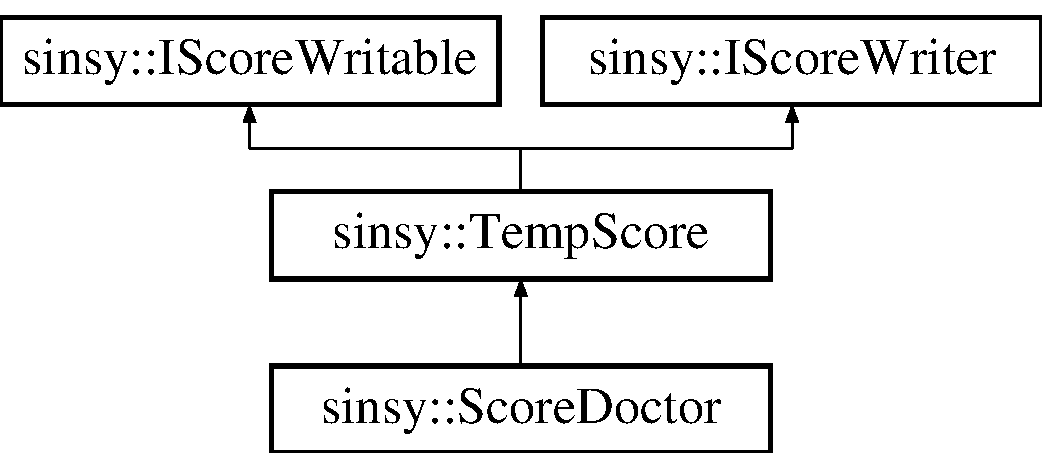
\includegraphics[height=3.000000cm]{classsinsy_1_1ScoreDoctor}
\end{center}
\end{figure}
\subsection*{\-Public \-Member \-Functions}
\begin{DoxyCompactItemize}
\item 
\hypertarget{classsinsy_1_1ScoreDoctor_a030b982f196fb69ee5b03616c12c7935}{\hyperlink{classsinsy_1_1ScoreDoctor_a030b982f196fb69ee5b03616c12c7935}{\-Score\-Doctor} ()}\label{classsinsy_1_1ScoreDoctor_a030b982f196fb69ee5b03616c12c7935}

\begin{DoxyCompactList}\small\item\em constructor \end{DoxyCompactList}\item 
\hypertarget{classsinsy_1_1ScoreDoctor_a2723d156fcf1731e4aeba260a92092e9}{virtual \hyperlink{classsinsy_1_1ScoreDoctor_a2723d156fcf1731e4aeba260a92092e9}{$\sim$\-Score\-Doctor} ()}\label{classsinsy_1_1ScoreDoctor_a2723d156fcf1731e4aeba260a92092e9}

\begin{DoxyCompactList}\small\item\em destructor \end{DoxyCompactList}\item 
\hypertarget{classsinsy_1_1ScoreDoctor_adf4d4ee66366758b84722cfaf11b83b3}{virtual void \hyperlink{classsinsy_1_1ScoreDoctor_adf4d4ee66366758b84722cfaf11b83b3}{add\-Note} (const \hyperlink{classsinsy_1_1Note}{\-Note} \&)}\label{classsinsy_1_1ScoreDoctor_adf4d4ee66366758b84722cfaf11b83b3}

\begin{DoxyCompactList}\small\item\em add note \end{DoxyCompactList}\end{DoxyCompactItemize}


\-The documentation for this class was generated from the following files\-:\begin{DoxyCompactItemize}
\item 
lib/temporary/\-Score\-Doctor.\-h\item 
lib/temporary/\-Score\-Doctor.\-cpp\end{DoxyCompactItemize}

\hypertarget{classsinsy_1_1ScorePosition}{\section{sinsy\-:\-:\-Score\-Position \-Class \-Reference}
\label{classsinsy_1_1ScorePosition}\index{sinsy\-::\-Score\-Position@{sinsy\-::\-Score\-Position}}
}
\subsection*{\-Public \-Member \-Functions}
\begin{DoxyCompactItemize}
\item 
\hypertarget{classsinsy_1_1ScorePosition_a351cf7880a457353b82f5aca418c40ce}{\hyperlink{classsinsy_1_1ScorePosition_a351cf7880a457353b82f5aca418c40ce}{\-Score\-Position} ()}\label{classsinsy_1_1ScorePosition_a351cf7880a457353b82f5aca418c40ce}

\begin{DoxyCompactList}\small\item\em constructor \end{DoxyCompactList}\item 
\hypertarget{classsinsy_1_1ScorePosition_ae1198c95e91e4067844c57c123a0baa0}{\hyperlink{classsinsy_1_1ScorePosition_ae1198c95e91e4067844c57c123a0baa0}{\-Score\-Position} (size\-\_\-t m)}\label{classsinsy_1_1ScorePosition_ae1198c95e91e4067844c57c123a0baa0}

\begin{DoxyCompactList}\small\item\em constructor \end{DoxyCompactList}\item 
\hypertarget{classsinsy_1_1ScorePosition_ae12829aaa62b2cc608159e6e1c9fc873}{\hyperlink{classsinsy_1_1ScorePosition_ae12829aaa62b2cc608159e6e1c9fc873}{\-Score\-Position} (size\-\_\-t m, size\-\_\-t n, size\-\_\-t d)}\label{classsinsy_1_1ScorePosition_ae12829aaa62b2cc608159e6e1c9fc873}

\begin{DoxyCompactList}\small\item\em constructor \end{DoxyCompactList}\item 
\hypertarget{classsinsy_1_1ScorePosition_a802bf7f9e230ba5d5880af9d79bf4a99}{\hyperlink{classsinsy_1_1ScorePosition_a802bf7f9e230ba5d5880af9d79bf4a99}{\-Score\-Position} (const \hyperlink{classsinsy_1_1ScorePosition}{\-Score\-Position} \&obj)}\label{classsinsy_1_1ScorePosition_a802bf7f9e230ba5d5880af9d79bf4a99}

\begin{DoxyCompactList}\small\item\em copy constructor \end{DoxyCompactList}\item 
\hypertarget{classsinsy_1_1ScorePosition_ae6400e1ae35a3bbd079593e0cff8773d}{virtual \hyperlink{classsinsy_1_1ScorePosition_ae6400e1ae35a3bbd079593e0cff8773d}{$\sim$\-Score\-Position} ()}\label{classsinsy_1_1ScorePosition_ae6400e1ae35a3bbd079593e0cff8773d}

\begin{DoxyCompactList}\small\item\em destructor \end{DoxyCompactList}\item 
\hypertarget{classsinsy_1_1ScorePosition_aa14e036a987d6b14eb25074beb3bfdee}{\hyperlink{classsinsy_1_1ScorePosition}{\-Score\-Position} \& \hyperlink{classsinsy_1_1ScorePosition_aa14e036a987d6b14eb25074beb3bfdee}{operator=} (const \hyperlink{classsinsy_1_1ScorePosition}{\-Score\-Position} \&)}\label{classsinsy_1_1ScorePosition_aa14e036a987d6b14eb25074beb3bfdee}

\begin{DoxyCompactList}\small\item\em assignment operator \end{DoxyCompactList}\item 
\hypertarget{classsinsy_1_1ScorePosition_ae54a343ad9c263287f9bf83811b87cf1}{size\-\_\-t \hyperlink{classsinsy_1_1ScorePosition_ae54a343ad9c263287f9bf83811b87cf1}{get\-Measure} () const }\label{classsinsy_1_1ScorePosition_ae54a343ad9c263287f9bf83811b87cf1}

\begin{DoxyCompactList}\small\item\em get measure \end{DoxyCompactList}\item 
\hypertarget{classsinsy_1_1ScorePosition_a88f706577270a8804f054aafe259a79f}{size\-\_\-t \hyperlink{classsinsy_1_1ScorePosition_a88f706577270a8804f054aafe259a79f}{get\-Numerator} () const }\label{classsinsy_1_1ScorePosition_a88f706577270a8804f054aafe259a79f}

\begin{DoxyCompactList}\small\item\em get numerator \end{DoxyCompactList}\item 
\hypertarget{classsinsy_1_1ScorePosition_a32949ba0558fd64faa80ebb3f40e44ff}{size\-\_\-t \hyperlink{classsinsy_1_1ScorePosition_a32949ba0558fd64faa80ebb3f40e44ff}{get\-Denominator} () const }\label{classsinsy_1_1ScorePosition_a32949ba0558fd64faa80ebb3f40e44ff}

\begin{DoxyCompactList}\small\item\em get denominator \end{DoxyCompactList}\end{DoxyCompactItemize}


\-The documentation for this class was generated from the following files\-:\begin{DoxyCompactItemize}
\item 
lib/score/\-Score\-Position.\-h\item 
lib/score/\-Score\-Position.\-cpp\end{DoxyCompactItemize}

\hypertarget{classsinsy_1_1SinsyImpl}{\section{sinsy\-:\-:\-Sinsy\-Impl \-Class \-Reference}
\label{classsinsy_1_1SinsyImpl}\index{sinsy\-::\-Sinsy\-Impl@{sinsy\-::\-Sinsy\-Impl}}
}
\-Inheritance diagram for sinsy\-:\-:\-Sinsy\-Impl\-:\begin{figure}[H]
\begin{center}
\leavevmode
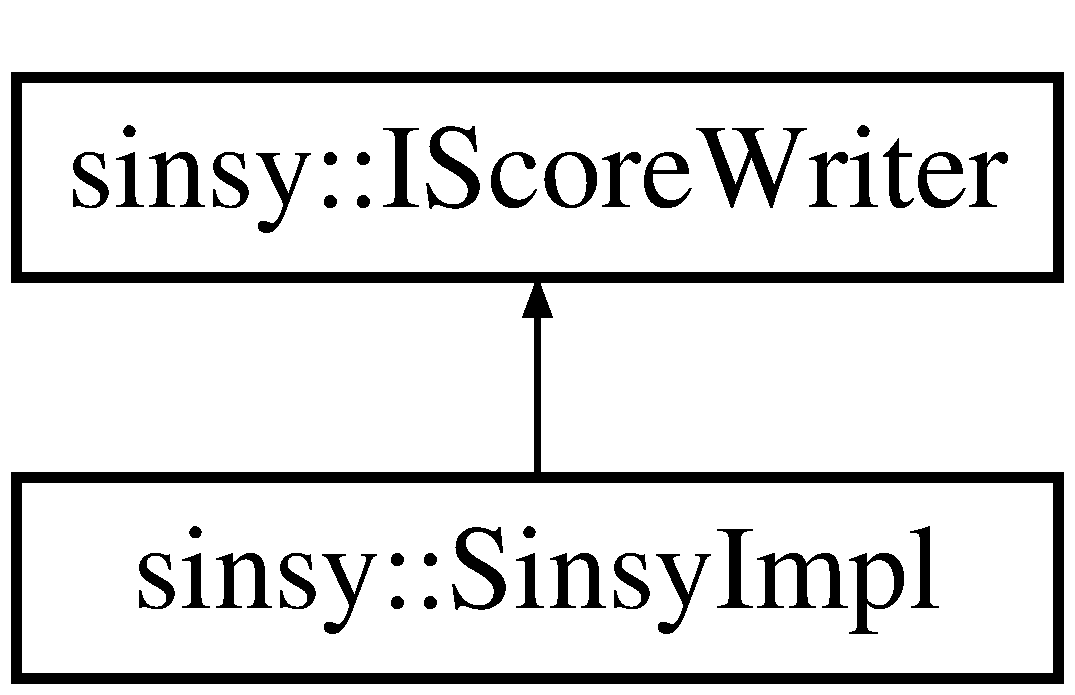
\includegraphics[height=2.000000cm]{classsinsy_1_1SinsyImpl}
\end{center}
\end{figure}
\subsection*{\-Public \-Member \-Functions}
\begin{DoxyCompactItemize}
\item 
\hypertarget{classsinsy_1_1SinsyImpl_a0d7a0552a3b60f4acc1e70bf87ae0efa}{\hyperlink{classsinsy_1_1SinsyImpl_a0d7a0552a3b60f4acc1e70bf87ae0efa}{\-Sinsy\-Impl} ()}\label{classsinsy_1_1SinsyImpl_a0d7a0552a3b60f4acc1e70bf87ae0efa}

\begin{DoxyCompactList}\small\item\em constructor \end{DoxyCompactList}\item 
\hypertarget{classsinsy_1_1SinsyImpl_acc760f5741befb97c06bd9347c6ec2b8}{virtual \hyperlink{classsinsy_1_1SinsyImpl_acc760f5741befb97c06bd9347c6ec2b8}{$\sim$\-Sinsy\-Impl} ()}\label{classsinsy_1_1SinsyImpl_acc760f5741befb97c06bd9347c6ec2b8}

\begin{DoxyCompactList}\small\item\em destructor \end{DoxyCompactList}\item 
\hypertarget{classsinsy_1_1SinsyImpl_a2d10481fda8da2cdb0374620371d535e}{bool \hyperlink{classsinsy_1_1SinsyImpl_a2d10481fda8da2cdb0374620371d535e}{set\-Languages} (const std\-::string \&languages, const std\-::string \&dir\-Path)}\label{classsinsy_1_1SinsyImpl_a2d10481fda8da2cdb0374620371d535e}

\begin{DoxyCompactList}\small\item\em set languages \end{DoxyCompactList}\item 
\hypertarget{classsinsy_1_1SinsyImpl_ac6db392238ea47e3e37a282a1c0ded5b}{bool \hyperlink{classsinsy_1_1SinsyImpl_ac6db392238ea47e3e37a282a1c0ded5b}{load\-Voices} (const std\-::vector$<$ std\-::string $>$ \&voices)}\label{classsinsy_1_1SinsyImpl_ac6db392238ea47e3e37a282a1c0ded5b}

\begin{DoxyCompactList}\small\item\em load voice files \end{DoxyCompactList}\item 
\hypertarget{classsinsy_1_1SinsyImpl_a702da6b5e69fb27ba595f46c945314f6}{void \hyperlink{classsinsy_1_1SinsyImpl_a702da6b5e69fb27ba595f46c945314f6}{set\-Encoding} (const std\-::string \&encoding)}\label{classsinsy_1_1SinsyImpl_a702da6b5e69fb27ba595f46c945314f6}

\begin{DoxyCompactList}\small\item\em set encoding \end{DoxyCompactList}\item 
\hypertarget{classsinsy_1_1SinsyImpl_a254416e5a9315c3f0f37c6dac9a0402e}{void \hyperlink{classsinsy_1_1SinsyImpl_a254416e5a9315c3f0f37c6dac9a0402e}{change\-Key} (const \hyperlink{classsinsy_1_1Key}{\-Key} \&key)}\label{classsinsy_1_1SinsyImpl_a254416e5a9315c3f0f37c6dac9a0402e}

\begin{DoxyCompactList}\small\item\em add key mark \end{DoxyCompactList}\item 
\hypertarget{classsinsy_1_1SinsyImpl_a7d21a316b514633fef6ac3c1c600fb84}{void \hyperlink{classsinsy_1_1SinsyImpl_a7d21a316b514633fef6ac3c1c600fb84}{change\-Beat} (const \hyperlink{classsinsy_1_1Beat}{\-Beat} \&beat)}\label{classsinsy_1_1SinsyImpl_a7d21a316b514633fef6ac3c1c600fb84}

\begin{DoxyCompactList}\small\item\em change beat \-: default beat mark is 4/4 \end{DoxyCompactList}\item 
\hypertarget{classsinsy_1_1SinsyImpl_a6f88bda91b47135291d9c38bd484fca5}{void \hyperlink{classsinsy_1_1SinsyImpl_a6f88bda91b47135291d9c38bd484fca5}{change\-Tempo} (double tempo)}\label{classsinsy_1_1SinsyImpl_a6f88bda91b47135291d9c38bd484fca5}

\begin{DoxyCompactList}\small\item\em change tempo \-: default tempo is 100bps \end{DoxyCompactList}\item 
\hypertarget{classsinsy_1_1SinsyImpl_a2443b028208d4d3bf1b191505950714c}{void \hyperlink{classsinsy_1_1SinsyImpl_a2443b028208d4d3bf1b191505950714c}{change\-Dynamics} (const \hyperlink{classsinsy_1_1Dynamics}{\-Dynamics} \&dynamics)}\label{classsinsy_1_1SinsyImpl_a2443b028208d4d3bf1b191505950714c}

\begin{DoxyCompactList}\small\item\em change dynamics (sudden changes) \end{DoxyCompactList}\item 
\hypertarget{classsinsy_1_1SinsyImpl_ae74148d756d94d12acfc4026f0ef0629}{void \hyperlink{classsinsy_1_1SinsyImpl_ae74148d756d94d12acfc4026f0ef0629}{start\-Crescendo} ()}\label{classsinsy_1_1SinsyImpl_ae74148d756d94d12acfc4026f0ef0629}

\begin{DoxyCompactList}\small\item\em start crescendo \end{DoxyCompactList}\item 
\hypertarget{classsinsy_1_1SinsyImpl_aae477f82fd122c8182f58eee6aa4850c}{void \hyperlink{classsinsy_1_1SinsyImpl_aae477f82fd122c8182f58eee6aa4850c}{stop\-Crescendo} ()}\label{classsinsy_1_1SinsyImpl_aae477f82fd122c8182f58eee6aa4850c}

\begin{DoxyCompactList}\small\item\em stop crescendo \end{DoxyCompactList}\item 
\hypertarget{classsinsy_1_1SinsyImpl_ae691d4395d2534246111c044110290f1}{void \hyperlink{classsinsy_1_1SinsyImpl_ae691d4395d2534246111c044110290f1}{start\-Diminuendo} ()}\label{classsinsy_1_1SinsyImpl_ae691d4395d2534246111c044110290f1}

\begin{DoxyCompactList}\small\item\em start diminuendo \end{DoxyCompactList}\item 
\hypertarget{classsinsy_1_1SinsyImpl_ac46c1d8a384f77ef76ba9ec374515515}{void \hyperlink{classsinsy_1_1SinsyImpl_ac46c1d8a384f77ef76ba9ec374515515}{stop\-Diminuendo} ()}\label{classsinsy_1_1SinsyImpl_ac46c1d8a384f77ef76ba9ec374515515}

\begin{DoxyCompactList}\small\item\em stop diminuendo \end{DoxyCompactList}\item 
\hypertarget{classsinsy_1_1SinsyImpl_aebc0e336dd09e5418cad4df9066dcd3e}{void \hyperlink{classsinsy_1_1SinsyImpl_aebc0e336dd09e5418cad4df9066dcd3e}{add\-Note} (const \hyperlink{classsinsy_1_1Note}{\-Note} \&note)}\label{classsinsy_1_1SinsyImpl_aebc0e336dd09e5418cad4df9066dcd3e}

\begin{DoxyCompactList}\small\item\em add note to end of score \end{DoxyCompactList}\item 
\hypertarget{classsinsy_1_1SinsyImpl_a845c7c596b66036f2d335b738609751b}{void \hyperlink{classsinsy_1_1SinsyImpl_a845c7c596b66036f2d335b738609751b}{write} (\hyperlink{classsinsy_1_1IScoreWritable}{\-I\-Score\-Writable} \&maker) const }\label{classsinsy_1_1SinsyImpl_a845c7c596b66036f2d335b738609751b}

\begin{DoxyCompactList}\small\item\em write score to given \hyperlink{classsinsy_1_1IScoreWritable}{\-I\-Score\-Writable} object \end{DoxyCompactList}\item 
\hypertarget{classsinsy_1_1SinsyImpl_a8c078864a93020ecde8e2ef7ef937bc8}{bool \hyperlink{classsinsy_1_1SinsyImpl_a8c078864a93020ecde8e2ef7ef937bc8}{set\-Alpha} (double alpha)}\label{classsinsy_1_1SinsyImpl_a8c078864a93020ecde8e2ef7ef937bc8}

\begin{DoxyCompactList}\small\item\em set alpha for synthesis \end{DoxyCompactList}\item 
\hypertarget{classsinsy_1_1SinsyImpl_ac5d68fb9e225a81ce7891ca55a325e37}{bool \hyperlink{classsinsy_1_1SinsyImpl_ac5d68fb9e225a81ce7891ca55a325e37}{set\-Volume} (double volume)}\label{classsinsy_1_1SinsyImpl_ac5d68fb9e225a81ce7891ca55a325e37}

\begin{DoxyCompactList}\small\item\em set volume for synthesis \end{DoxyCompactList}\item 
\hypertarget{classsinsy_1_1SinsyImpl_a1390773ced789ac13ec3711365456266}{bool \hyperlink{classsinsy_1_1SinsyImpl_a1390773ced789ac13ec3711365456266}{set\-Interpolation\-Weight} (size\-\_\-t index, double weight)}\label{classsinsy_1_1SinsyImpl_a1390773ced789ac13ec3711365456266}

\begin{DoxyCompactList}\small\item\em set interpolation weight for synthesis \end{DoxyCompactList}\item 
\hypertarget{classsinsy_1_1SinsyImpl_aaefd1b2092c4886a924540073e8794ba}{bool \hyperlink{classsinsy_1_1SinsyImpl_aaefd1b2092c4886a924540073e8794ba}{synthesize} (\hyperlink{classsinsy_1_1SynthConditionImpl}{\-Synth\-Condition\-Impl} \&condition)}\label{classsinsy_1_1SinsyImpl_aaefd1b2092c4886a924540073e8794ba}

\begin{DoxyCompactList}\small\item\em synthesize \end{DoxyCompactList}\item 
\hypertarget{classsinsy_1_1SinsyImpl_a8b26c8e6c77536ec158a353713523e1b}{bool \hyperlink{classsinsy_1_1SinsyImpl_a8b26c8e6c77536ec158a353713523e1b}{printlabel} (\hyperlink{classsinsy_1_1SynthConditionImpl}{\-Synth\-Condition\-Impl} \&condition)}\label{classsinsy_1_1SinsyImpl_a8b26c8e6c77536ec158a353713523e1b}

\begin{DoxyCompactList}\small\item\em synthesize \end{DoxyCompactList}\item 
\hypertarget{classsinsy_1_1SinsyImpl_acd437b473026f2a15dbf628af6248095}{void \hyperlink{classsinsy_1_1SinsyImpl_acd437b473026f2a15dbf628af6248095}{stop} ()}\label{classsinsy_1_1SinsyImpl_acd437b473026f2a15dbf628af6248095}

\begin{DoxyCompactList}\small\item\em stop synthesizing \end{DoxyCompactList}\item 
\hypertarget{classsinsy_1_1SinsyImpl_a524a03c6557f90dce77bec865f12c97d}{void \hyperlink{classsinsy_1_1SinsyImpl_a524a03c6557f90dce77bec865f12c97d}{reset\-Stop\-Flag} ()}\label{classsinsy_1_1SinsyImpl_a524a03c6557f90dce77bec865f12c97d}

\begin{DoxyCompactList}\small\item\em reset stop flag \end{DoxyCompactList}\item 
\hypertarget{classsinsy_1_1SinsyImpl_a9aac96b24c7dfa8fa874da47cfd5ffac}{void \hyperlink{classsinsy_1_1SinsyImpl_a9aac96b24c7dfa8fa874da47cfd5ffac}{clear\-Score} ()}\label{classsinsy_1_1SinsyImpl_a9aac96b24c7dfa8fa874da47cfd5ffac}

\begin{DoxyCompactList}\small\item\em clear score \end{DoxyCompactList}\item 
\hypertarget{classsinsy_1_1SinsyImpl_ac1e56b876037a7709108cffe6a170ff3}{bool \hyperlink{classsinsy_1_1SinsyImpl_ac1e56b876037a7709108cffe6a170ff3}{load\-Score\-From\-Music\-X\-M\-L} (\hyperlink{classsinsy_1_1InputFile}{\-Input\-File} \&xml)}\label{classsinsy_1_1SinsyImpl_ac1e56b876037a7709108cffe6a170ff3}

\begin{DoxyCompactList}\small\item\em load score from \-Music\-X\-M\-L \end{DoxyCompactList}\item 
\hypertarget{classsinsy_1_1SinsyImpl_a2cae49dcd06ba100b788e2d28f0060c6}{bool {\bfseries set\-X\-M\-L\-Data} (const \hyperlink{classsinsy_1_1XmlData}{\-Xml\-Data} $\ast$xdata)}\label{classsinsy_1_1SinsyImpl_a2cae49dcd06ba100b788e2d28f0060c6}

\item 
\hypertarget{classsinsy_1_1SinsyImpl_ab4aef01229731bd24f9cd8c1f98a5f39}{const \hyperlink{classsinsy_1_1XmlData}{\-Xml\-Data} $\ast$ {\bfseries get\-X\-M\-L\-Data} ()}\label{classsinsy_1_1SinsyImpl_ab4aef01229731bd24f9cd8c1f98a5f39}

\item 
\hypertarget{classsinsy_1_1SinsyImpl_ac7ffea79eb90ff782db69a9824aadcff}{bool \hyperlink{classsinsy_1_1SinsyImpl_ac7ffea79eb90ff782db69a9824aadcff}{save\-Score\-To\-Music\-X\-M\-L} (const std\-::string \&xml)}\label{classsinsy_1_1SinsyImpl_ac7ffea79eb90ff782db69a9824aadcff}

\begin{DoxyCompactList}\small\item\em save score to \-Music\-X\-M\-L \end{DoxyCompactList}\item 
\hypertarget{classsinsy_1_1SinsyImpl_a9b15d5674ac1189c9e9abd76cddcaa62}{bool \hyperlink{classsinsy_1_1SinsyImpl_a9b15d5674ac1189c9e9abd76cddcaa62}{save\-Score\-To\-Music\-X\-M\-L\-Phon} (const std\-::string \&xml)}\label{classsinsy_1_1SinsyImpl_a9b15d5674ac1189c9e9abd76cddcaa62}

\begin{DoxyCompactList}\small\item\em save score to \-Music\-X\-M\-L \end{DoxyCompactList}\end{DoxyCompactItemize}


\-The documentation for this class was generated from the following file\-:\begin{DoxyCompactItemize}
\item 
lib/\-Sinsy.\-cpp\end{DoxyCompactItemize}

\hypertarget{classsinsy_1_1Slur}{\section{sinsy\-:\-:\-Slur \-Class \-Reference}
\label{classsinsy_1_1Slur}\index{sinsy\-::\-Slur@{sinsy\-::\-Slur}}
}
\subsection*{\-Public \-Member \-Functions}
\begin{DoxyCompactItemize}
\item 
\hypertarget{classsinsy_1_1Slur_aba0fcae139a72d06ecfafa10f41e672b}{\hyperlink{classsinsy_1_1Slur_aba0fcae139a72d06ecfafa10f41e672b}{\-Slur} ()}\label{classsinsy_1_1Slur_aba0fcae139a72d06ecfafa10f41e672b}

\begin{DoxyCompactList}\small\item\em constructor \end{DoxyCompactList}\item 
\hypertarget{classsinsy_1_1Slur_a3afc452caaf08653f482f590c754dc17}{\hyperlink{classsinsy_1_1Slur_a3afc452caaf08653f482f590c754dc17}{\-Slur} (const \hyperlink{classsinsy_1_1Slur}{\-Slur} \&obj)}\label{classsinsy_1_1Slur_a3afc452caaf08653f482f590c754dc17}

\begin{DoxyCompactList}\small\item\em copy constructor \end{DoxyCompactList}\item 
\hypertarget{classsinsy_1_1Slur_a3db24c2ec21ab6bd61913b0738d53fb7}{virtual \hyperlink{classsinsy_1_1Slur_a3db24c2ec21ab6bd61913b0738d53fb7}{$\sim$\-Slur} ()}\label{classsinsy_1_1Slur_a3db24c2ec21ab6bd61913b0738d53fb7}

\begin{DoxyCompactList}\small\item\em destructor \end{DoxyCompactList}\item 
\hypertarget{classsinsy_1_1Slur_a97b57041baff294fddef94bf75d04ee6}{\hyperlink{classsinsy_1_1Slur}{\-Slur} \& \hyperlink{classsinsy_1_1Slur_a97b57041baff294fddef94bf75d04ee6}{operator=} (const \hyperlink{classsinsy_1_1Slur}{\-Slur} \&obj)}\label{classsinsy_1_1Slur_a97b57041baff294fddef94bf75d04ee6}

\begin{DoxyCompactList}\small\item\em assignment operator \end{DoxyCompactList}\item 
\hypertarget{classsinsy_1_1Slur_a9a0abb5593bae4c3956d9be7af643d29}{void \hyperlink{classsinsy_1_1Slur_a9a0abb5593bae4c3956d9be7af643d29}{add\-Start} (int number)}\label{classsinsy_1_1Slur_a9a0abb5593bae4c3956d9be7af643d29}

\begin{DoxyCompactList}\small\item\em add start \end{DoxyCompactList}\item 
\hypertarget{classsinsy_1_1Slur_a98162ae58b2c8b6306b93dbae9f9a352}{void \hyperlink{classsinsy_1_1Slur_a98162ae58b2c8b6306b93dbae9f9a352}{add\-Stop} (int number)}\label{classsinsy_1_1Slur_a98162ae58b2c8b6306b93dbae9f9a352}

\begin{DoxyCompactList}\small\item\em add stop \end{DoxyCompactList}\item 
\hypertarget{classsinsy_1_1Slur_a46e79fde5bc86ea0cdc3a2fc9c4f6106}{bool \hyperlink{classsinsy_1_1Slur_a46e79fde5bc86ea0cdc3a2fc9c4f6106}{no\-Slur} () const }\label{classsinsy_1_1Slur_a46e79fde5bc86ea0cdc3a2fc9c4f6106}

\begin{DoxyCompactList}\small\item\em no slur or not \end{DoxyCompactList}\item 
\hypertarget{classsinsy_1_1Slur_a270b3b4a1ef3046778aa450f7c8fd6b2}{void \hyperlink{classsinsy_1_1Slur_a270b3b4a1ef3046778aa450f7c8fd6b2}{merge\-To} (\hyperlink{classsinsy_1_1Slur}{\-Slur} \&slur) const }\label{classsinsy_1_1Slur_a270b3b4a1ef3046778aa450f7c8fd6b2}

\begin{DoxyCompactList}\small\item\em merge to another slur \end{DoxyCompactList}\item 
\hypertarget{classsinsy_1_1Slur_a5e500b2c0b5edd2f507018e42fab26e7}{void \hyperlink{classsinsy_1_1Slur_a5e500b2c0b5edd2f507018e42fab26e7}{clear} ()}\label{classsinsy_1_1Slur_a5e500b2c0b5edd2f507018e42fab26e7}

\begin{DoxyCompactList}\small\item\em clear \end{DoxyCompactList}\end{DoxyCompactItemize}
\subsection*{\-Friends}
\begin{DoxyCompactItemize}
\item 
\hypertarget{classsinsy_1_1Slur_a8ff2ab21451a4b94bffe63cef60dce96}{std\-::ostream \& \hyperlink{classsinsy_1_1Slur_a8ff2ab21451a4b94bffe63cef60dce96}{operator$<$$<$} (std\-::ostream \&os, const \hyperlink{classsinsy_1_1Slur}{\-Slur} \&slur)}\label{classsinsy_1_1Slur_a8ff2ab21451a4b94bffe63cef60dce96}

\begin{DoxyCompactList}\small\item\em to stream \end{DoxyCompactList}\end{DoxyCompactItemize}


\-The documentation for this class was generated from the following files\-:\begin{DoxyCompactItemize}
\item 
lib/score/\-Slur.\-h\item 
lib/score/\-Slur.\-cpp\end{DoxyCompactItemize}

\hypertarget{classsinsy_1_1StreamException}{\section{sinsy\-:\-:\-Stream\-Exception \-Class \-Reference}
\label{classsinsy_1_1StreamException}\index{sinsy\-::\-Stream\-Exception@{sinsy\-::\-Stream\-Exception}}
}
\subsection*{\-Public \-Member \-Functions}
\begin{DoxyCompactItemize}
\item 
\hypertarget{classsinsy_1_1StreamException_a397caf8a6766811aa67bdfd7856b1c7d}{\hyperlink{classsinsy_1_1StreamException_a397caf8a6766811aa67bdfd7856b1c7d}{\-Stream\-Exception} (const std\-::string \&msg)}\label{classsinsy_1_1StreamException_a397caf8a6766811aa67bdfd7856b1c7d}

\begin{DoxyCompactList}\small\item\em constructor \end{DoxyCompactList}\item 
\hypertarget{classsinsy_1_1StreamException_a60ede7f62c743c7e9e8dc6e92813f227}{virtual \hyperlink{classsinsy_1_1StreamException_a60ede7f62c743c7e9e8dc6e92813f227}{$\sim$\-Stream\-Exception} ()  throw ()}\label{classsinsy_1_1StreamException_a60ede7f62c743c7e9e8dc6e92813f227}

\begin{DoxyCompactList}\small\item\em destructor \end{DoxyCompactList}\end{DoxyCompactItemize}


\-The documentation for this class was generated from the following file\-:\begin{DoxyCompactItemize}
\item 
lib/util/\-Stream\-Exception.\-h\end{DoxyCompactItemize}

\hypertarget{classsinsy_1_1StringTokenizer}{\section{sinsy\-:\-:\-String\-Tokenizer \-Class \-Reference}
\label{classsinsy_1_1StringTokenizer}\index{sinsy\-::\-String\-Tokenizer@{sinsy\-::\-String\-Tokenizer}}
}
\subsection*{\-Public \-Member \-Functions}
\begin{DoxyCompactItemize}
\item 
\hypertarget{classsinsy_1_1StringTokenizer_a9e7a76b341939bc5b97daa75134da1ff}{\hyperlink{classsinsy_1_1StringTokenizer_a9e7a76b341939bc5b97daa75134da1ff}{\-String\-Tokenizer} (const \-::std\-::string \&str, const std\-::string \&separator)}\label{classsinsy_1_1StringTokenizer_a9e7a76b341939bc5b97daa75134da1ff}

\begin{DoxyCompactList}\small\item\em constructor \end{DoxyCompactList}\item 
\hypertarget{classsinsy_1_1StringTokenizer_a74f663e102f0d731990494c0d7fd8803}{{\bfseries \-String\-Tokenizer} (const std\-::string \&str, const std\-::string \&separator, bool match)}\label{classsinsy_1_1StringTokenizer_a74f663e102f0d731990494c0d7fd8803}

\item 
\hypertarget{classsinsy_1_1StringTokenizer_a26a59cd69f871ace17ec831e1508b377}{virtual \hyperlink{classsinsy_1_1StringTokenizer_a26a59cd69f871ace17ec831e1508b377}{$\sim$\-String\-Tokenizer} ()}\label{classsinsy_1_1StringTokenizer_a26a59cd69f871ace17ec831e1508b377}

\begin{DoxyCompactList}\small\item\em destructor \end{DoxyCompactList}\item 
\hypertarget{classsinsy_1_1StringTokenizer_a85bda635b73d7321e769f935c8ceb2e0}{std\-::string \hyperlink{classsinsy_1_1StringTokenizer_a85bda635b73d7321e769f935c8ceb2e0}{at} (size\-\_\-t idx) const }\label{classsinsy_1_1StringTokenizer_a85bda635b73d7321e769f935c8ceb2e0}

\begin{DoxyCompactList}\small\item\em access at element of idx \end{DoxyCompactList}\item 
\hypertarget{classsinsy_1_1StringTokenizer_a920b9028afe112760e4c088a2c378c5f}{size\-\_\-t \hyperlink{classsinsy_1_1StringTokenizer_a920b9028afe112760e4c088a2c378c5f}{size} () const }\label{classsinsy_1_1StringTokenizer_a920b9028afe112760e4c088a2c378c5f}

\begin{DoxyCompactList}\small\item\em get size \end{DoxyCompactList}\end{DoxyCompactItemize}


\-The documentation for this class was generated from the following files\-:\begin{DoxyCompactItemize}
\item 
lib/util/\-String\-Tokenizer.\-h\item 
lib/util/\-String\-Tokenizer.\-cpp\end{DoxyCompactItemize}

\hypertarget{classsinsy_1_1Syllabic}{\section{sinsy\-:\-:\-Syllabic \-Class \-Reference}
\label{classsinsy_1_1Syllabic}\index{sinsy\-::\-Syllabic@{sinsy\-::\-Syllabic}}
}
\subsection*{\-Public \-Member \-Functions}
\begin{DoxyCompactItemize}
\item 
\hypertarget{classsinsy_1_1Syllabic_a422090601b0c5dedcb6a302f75ff54e9}{\hyperlink{classsinsy_1_1Syllabic_a422090601b0c5dedcb6a302f75ff54e9}{\-Syllabic} ()}\label{classsinsy_1_1Syllabic_a422090601b0c5dedcb6a302f75ff54e9}

\begin{DoxyCompactList}\small\item\em constructor \end{DoxyCompactList}\item 
\hypertarget{classsinsy_1_1Syllabic_a3e5334cbfc18deb457430f3bce03fe8a}{\hyperlink{classsinsy_1_1Syllabic_a3e5334cbfc18deb457430f3bce03fe8a}{\-Syllabic} (const std\-::string \&str)}\label{classsinsy_1_1Syllabic_a3e5334cbfc18deb457430f3bce03fe8a}

\begin{DoxyCompactList}\small\item\em constructor \end{DoxyCompactList}\item 
\hypertarget{classsinsy_1_1Syllabic_a96d3a8a7b0da42ec0e9d0b5de6789012}{\hyperlink{classsinsy_1_1Syllabic_a96d3a8a7b0da42ec0e9d0b5de6789012}{\-Syllabic} (const \hyperlink{classsinsy_1_1Syllabic}{\-Syllabic} \&obj)}\label{classsinsy_1_1Syllabic_a96d3a8a7b0da42ec0e9d0b5de6789012}

\begin{DoxyCompactList}\small\item\em copy constructor \end{DoxyCompactList}\item 
\hypertarget{classsinsy_1_1Syllabic_a059a986d8f998a9d7c5da6479c732246}{virtual \hyperlink{classsinsy_1_1Syllabic_a059a986d8f998a9d7c5da6479c732246}{$\sim$\-Syllabic} ()}\label{classsinsy_1_1Syllabic_a059a986d8f998a9d7c5da6479c732246}

\begin{DoxyCompactList}\small\item\em destructor \end{DoxyCompactList}\item 
\hypertarget{classsinsy_1_1Syllabic_a68868d0713d7220d522b7fac79784329}{\hyperlink{classsinsy_1_1Syllabic}{\-Syllabic} \& \hyperlink{classsinsy_1_1Syllabic_a68868d0713d7220d522b7fac79784329}{operator=} (const \hyperlink{classsinsy_1_1Syllabic}{\-Syllabic} \&obj)}\label{classsinsy_1_1Syllabic_a68868d0713d7220d522b7fac79784329}

\begin{DoxyCompactList}\small\item\em assignment operator \end{DoxyCompactList}\item 
\hypertarget{classsinsy_1_1Syllabic_a869e1923c8dd9a52449c85e8b462d610}{bool \hyperlink{classsinsy_1_1Syllabic_a869e1923c8dd9a52449c85e8b462d610}{operator==} (const \hyperlink{classsinsy_1_1Syllabic}{\-Syllabic} \&obj) const }\label{classsinsy_1_1Syllabic_a869e1923c8dd9a52449c85e8b462d610}

\begin{DoxyCompactList}\small\item\em equal \end{DoxyCompactList}\item 
\hypertarget{classsinsy_1_1Syllabic_a9b4292492ae66154915562a217c2a301}{bool \hyperlink{classsinsy_1_1Syllabic_a9b4292492ae66154915562a217c2a301}{operator!=} (const \hyperlink{classsinsy_1_1Syllabic}{\-Syllabic} \&obj) const }\label{classsinsy_1_1Syllabic_a9b4292492ae66154915562a217c2a301}

\begin{DoxyCompactList}\small\item\em not equal \end{DoxyCompactList}\item 
void \hyperlink{classsinsy_1_1Syllabic_a35c59408a52e112e2529dc0c93e5fc12}{set} (const std\-::string \&s)
\begin{DoxyCompactList}\small\item\em set syllabic \end{DoxyCompactList}\item 
\hypertarget{classsinsy_1_1Syllabic_acc3876365a65187fe088a7f675b08c17}{const std\-::string \& \hyperlink{classsinsy_1_1Syllabic_acc3876365a65187fe088a7f675b08c17}{get} () const }\label{classsinsy_1_1Syllabic_acc3876365a65187fe088a7f675b08c17}

\begin{DoxyCompactList}\small\item\em get syllabic \end{DoxyCompactList}\end{DoxyCompactItemize}
\subsection*{\-Static \-Public \-Attributes}
\begin{DoxyCompactItemize}
\item 
\hypertarget{classsinsy_1_1Syllabic_a900ec1dbf9de3aa91ccb38e324676992}{static const \hyperlink{classsinsy_1_1Syllabic}{\-Syllabic} {\bfseries \-S\-I\-N\-G\-L\-E}}\label{classsinsy_1_1Syllabic_a900ec1dbf9de3aa91ccb38e324676992}

\item 
\hypertarget{classsinsy_1_1Syllabic_ab881b8fd1ba1d1d86770be53acb9c0f5}{static const \hyperlink{classsinsy_1_1Syllabic}{\-Syllabic} {\bfseries \-B\-E\-G\-I\-N}}\label{classsinsy_1_1Syllabic_ab881b8fd1ba1d1d86770be53acb9c0f5}

\item 
\hypertarget{classsinsy_1_1Syllabic_af79bcda00b0e13db794308389371ffca}{static const \hyperlink{classsinsy_1_1Syllabic}{\-Syllabic} {\bfseries \-E\-N\-D}}\label{classsinsy_1_1Syllabic_af79bcda00b0e13db794308389371ffca}

\item 
\hypertarget{classsinsy_1_1Syllabic_a355c30d25776b32a95a1868c3d29390a}{static const \hyperlink{classsinsy_1_1Syllabic}{\-Syllabic} {\bfseries \-M\-I\-D\-D\-L\-E}}\label{classsinsy_1_1Syllabic_a355c30d25776b32a95a1868c3d29390a}

\end{DoxyCompactItemize}


\subsection{\-Member \-Function \-Documentation}
\hypertarget{classsinsy_1_1Syllabic_a35c59408a52e112e2529dc0c93e5fc12}{\index{sinsy\-::\-Syllabic@{sinsy\-::\-Syllabic}!set@{set}}
\index{set@{set}!sinsy::Syllabic@{sinsy\-::\-Syllabic}}
\subsubsection[{set}]{\setlength{\rightskip}{0pt plus 5cm}void {\bf \-Syllabic\-::set} (
\begin{DoxyParamCaption}
\item[{const std\-::string \&}]{s}
\end{DoxyParamCaption}
)}}\label{classsinsy_1_1Syllabic_a35c59408a52e112e2529dc0c93e5fc12}


set syllabic 

set 

\-The documentation for this class was generated from the following files\-:\begin{DoxyCompactItemize}
\item 
lib/score/\-Syllabic.\-h\item 
lib/score/\-Syllabic.\-cpp\end{DoxyCompactItemize}

\hypertarget{classsinsy_1_1SyllableLabeler}{\section{sinsy\-:\-:\-Syllable\-Labeler \-Class \-Reference}
\label{classsinsy_1_1SyllableLabeler}\index{sinsy\-::\-Syllable\-Labeler@{sinsy\-::\-Syllable\-Labeler}}
}
\subsection*{\-Public \-Types}
\begin{DoxyCompactItemize}
\item 
\hypertarget{classsinsy_1_1SyllableLabeler_a4a55b1a946d8bde28811af03dac0b52a}{typedef std\-::vector\*
$<$ \hyperlink{classsinsy_1_1PhonemeLabeler}{\-Phoneme\-Labeler} $\ast$ $>$ {\bfseries \-List}}\label{classsinsy_1_1SyllableLabeler_a4a55b1a946d8bde28811af03dac0b52a}

\end{DoxyCompactItemize}
\subsection*{\-Public \-Member \-Functions}
\begin{DoxyCompactItemize}
\item 
\hypertarget{classsinsy_1_1SyllableLabeler_a91b3bff4ba682519268f7b9b1b477e45}{\hyperlink{classsinsy_1_1SyllableLabeler_a91b3bff4ba682519268f7b9b1b477e45}{\-Syllable\-Labeler} (const std\-::string \&lang)}\label{classsinsy_1_1SyllableLabeler_a91b3bff4ba682519268f7b9b1b477e45}

\begin{DoxyCompactList}\small\item\em constructor \end{DoxyCompactList}\item 
\hypertarget{classsinsy_1_1SyllableLabeler_a577205cd458a184e916c1308dbeeafe1}{virtual \hyperlink{classsinsy_1_1SyllableLabeler_a577205cd458a184e916c1308dbeeafe1}{$\sim$\-Syllable\-Labeler} ()}\label{classsinsy_1_1SyllableLabeler_a577205cd458a184e916c1308dbeeafe1}

\begin{DoxyCompactList}\small\item\em destructor \end{DoxyCompactList}\item 
\hypertarget{classsinsy_1_1SyllableLabeler_a162b6e74e23dafca1c14680fcf77446f}{virtual void \hyperlink{classsinsy_1_1SyllableLabeler_a162b6e74e23dafca1c14680fcf77446f}{set\-Label} (\hyperlink{classsinsy_1_1ISyllableLabel}{\-I\-Syllable\-Label} \&) const }\label{classsinsy_1_1SyllableLabeler_a162b6e74e23dafca1c14680fcf77446f}

\begin{DoxyCompactList}\small\item\em set label \end{DoxyCompactList}\item 
\hypertarget{classsinsy_1_1SyllableLabeler_ac8a4cfeb6b3c657b30d42f4470915523}{void \hyperlink{classsinsy_1_1SyllableLabeler_ac8a4cfeb6b3c657b30d42f4470915523}{add\-Child} (\hyperlink{classsinsy_1_1PhonemeLabeler}{\-Phoneme\-Labeler} $\ast$l)}\label{classsinsy_1_1SyllableLabeler_ac8a4cfeb6b3c657b30d42f4470915523}

\begin{DoxyCompactList}\small\item\em add phoneme \end{DoxyCompactList}\item 
\-List\-::const\-\_\-iterator \hyperlink{classsinsy_1_1SyllableLabeler_a49d114d213883cbeb6bc0c445ef36e7e}{child\-Begin} () const 
\begin{DoxyCompactList}\small\item\em get begin iterator of phonemes \end{DoxyCompactList}\item 
\hypertarget{classsinsy_1_1SyllableLabeler_a94ecf79a7f761d2d35e6d9cfe3d59938}{\-List\-::const\-\_\-iterator \hyperlink{classsinsy_1_1SyllableLabeler_a94ecf79a7f761d2d35e6d9cfe3d59938}{child\-End} () const }\label{classsinsy_1_1SyllableLabeler_a94ecf79a7f761d2d35e6d9cfe3d59938}

\begin{DoxyCompactList}\small\item\em get end interator of phonemes \end{DoxyCompactList}\item 
\hypertarget{classsinsy_1_1SyllableLabeler_a6ea10c283e358509c80006530a2dc8f8}{void \hyperlink{classsinsy_1_1SyllableLabeler_a6ea10c283e358509c80006530a2dc8f8}{set\-Info} (const std\-::string \&str)}\label{classsinsy_1_1SyllableLabeler_a6ea10c283e358509c80006530a2dc8f8}

\begin{DoxyCompactList}\small\item\em set language dependent information \end{DoxyCompactList}\item 
\hypertarget{classsinsy_1_1SyllableLabeler_a1c21b590f513e8f8a6762524cf7834a3}{void \hyperlink{classsinsy_1_1SyllableLabeler_a1c21b590f513e8f8a6762524cf7834a3}{set\-Idx\-In\-Note} (size\-\_\-t i)}\label{classsinsy_1_1SyllableLabeler_a1c21b590f513e8f8a6762524cf7834a3}

\begin{DoxyCompactList}\small\item\em set index in note \end{DoxyCompactList}\item 
\hypertarget{classsinsy_1_1SyllableLabeler_a98ae9f74c44def9b765b454ba6973d26}{void \hyperlink{classsinsy_1_1SyllableLabeler_a98ae9f74c44def9b765b454ba6973d26}{set\-Num\-In\-Note} (size\-\_\-t n)}\label{classsinsy_1_1SyllableLabeler_a98ae9f74c44def9b765b454ba6973d26}

\begin{DoxyCompactList}\small\item\em set number in note \end{DoxyCompactList}\item 
\hypertarget{classsinsy_1_1SyllableLabeler_af3b9b5f151d486b3558d7d3ec029ffc4}{void \hyperlink{classsinsy_1_1SyllableLabeler_af3b9b5f151d486b3558d7d3ec029ffc4}{set\-Phoneme\-Positions} ()}\label{classsinsy_1_1SyllableLabeler_af3b9b5f151d486b3558d7d3ec029ffc4}

\begin{DoxyCompactList}\small\item\em set phoneme positions \end{DoxyCompactList}\end{DoxyCompactItemize}


\subsection{\-Member \-Function \-Documentation}
\hypertarget{classsinsy_1_1SyllableLabeler_a49d114d213883cbeb6bc0c445ef36e7e}{\index{sinsy\-::\-Syllable\-Labeler@{sinsy\-::\-Syllable\-Labeler}!child\-Begin@{child\-Begin}}
\index{child\-Begin@{child\-Begin}!sinsy::SyllableLabeler@{sinsy\-::\-Syllable\-Labeler}}
\subsubsection[{child\-Begin}]{\setlength{\rightskip}{0pt plus 5cm}\-Syllable\-Labeler\-::\-List\-::const\-\_\-iterator {\bf \-Syllable\-Labeler\-::child\-Begin} (
\begin{DoxyParamCaption}
{}
\end{DoxyParamCaption}
) const}}\label{classsinsy_1_1SyllableLabeler_a49d114d213883cbeb6bc0c445ef36e7e}


get begin iterator of phonemes 

get begin interator of phonemes 

\-The documentation for this class was generated from the following files\-:\begin{DoxyCompactItemize}
\item 
lib/label/\-Syllable\-Labeler.\-h\item 
lib/label/\-Syllable\-Labeler.\-cpp\end{DoxyCompactItemize}

\hypertarget{classsinsy_1_1SynthConditionImpl}{\section{sinsy\-:\-:\-Synth\-Condition\-Impl \-Class \-Reference}
\label{classsinsy_1_1SynthConditionImpl}\index{sinsy\-::\-Synth\-Condition\-Impl@{sinsy\-::\-Synth\-Condition\-Impl}}
}
\subsection*{\-Public \-Member \-Functions}
\begin{DoxyCompactItemize}
\item 
\hypertarget{classsinsy_1_1SynthConditionImpl_aa97e00c31046727c71f0030412275b06}{\hyperlink{classsinsy_1_1SynthConditionImpl_aa97e00c31046727c71f0030412275b06}{\-Synth\-Condition\-Impl} ()}\label{classsinsy_1_1SynthConditionImpl_aa97e00c31046727c71f0030412275b06}

\begin{DoxyCompactList}\small\item\em constructor \end{DoxyCompactList}\item 
\hypertarget{classsinsy_1_1SynthConditionImpl_a75fad8152cafb1fc5dd529a9516d9051}{virtual \hyperlink{classsinsy_1_1SynthConditionImpl_a75fad8152cafb1fc5dd529a9516d9051}{$\sim$\-Synth\-Condition\-Impl} ()}\label{classsinsy_1_1SynthConditionImpl_a75fad8152cafb1fc5dd529a9516d9051}

\begin{DoxyCompactList}\small\item\em destructor \end{DoxyCompactList}\item 
\hypertarget{classsinsy_1_1SynthConditionImpl_a49863ab67d09dd96028abc325bcad3d4}{void \hyperlink{classsinsy_1_1SynthConditionImpl_a49863ab67d09dd96028abc325bcad3d4}{set\-Play\-Flag} ()}\label{classsinsy_1_1SynthConditionImpl_a49863ab67d09dd96028abc325bcad3d4}

\begin{DoxyCompactList}\small\item\em set play flag \end{DoxyCompactList}\item 
\hypertarget{classsinsy_1_1SynthConditionImpl_af36b8eb252a96d545b6fbdd5da5d6144}{void \hyperlink{classsinsy_1_1SynthConditionImpl_af36b8eb252a96d545b6fbdd5da5d6144}{unset\-Play\-Flag} ()}\label{classsinsy_1_1SynthConditionImpl_af36b8eb252a96d545b6fbdd5da5d6144}

\begin{DoxyCompactList}\small\item\em unset play flag \end{DoxyCompactList}\item 
\hypertarget{classsinsy_1_1SynthConditionImpl_adb799ad0576a025480dc05f29308e983}{void \hyperlink{classsinsy_1_1SynthConditionImpl_adb799ad0576a025480dc05f29308e983}{set\-Save\-File\-Path} (const std\-::string \&file\-Path)}\label{classsinsy_1_1SynthConditionImpl_adb799ad0576a025480dc05f29308e983}

\begin{DoxyCompactList}\small\item\em set file path to save \-R\-I\-F\-F format file \end{DoxyCompactList}\item 
\hypertarget{classsinsy_1_1SynthConditionImpl_ad432aebb654f006e0028d6193a3c13b2}{void \hyperlink{classsinsy_1_1SynthConditionImpl_ad432aebb654f006e0028d6193a3c13b2}{set\-Save\-Label\-File\-Path} (const std\-::string \&file\-Path)}\label{classsinsy_1_1SynthConditionImpl_ad432aebb654f006e0028d6193a3c13b2}

\begin{DoxyCompactList}\small\item\em set file path to save label format file \end{DoxyCompactList}\item 
std\-::string \hyperlink{classsinsy_1_1SynthConditionImpl_a2b2079d83850a92314fdf04e81ef058d}{get\-Save\-Label\-File\-Path} ()
\begin{DoxyCompactList}\small\item\em set file path to save label format file \end{DoxyCompactList}\item 
\hypertarget{classsinsy_1_1SynthConditionImpl_ae3117a16602776ab9f568c5a8569f455}{void \hyperlink{classsinsy_1_1SynthConditionImpl_ae3117a16602776ab9f568c5a8569f455}{unset\-Save\-File\-Path} ()}\label{classsinsy_1_1SynthConditionImpl_ae3117a16602776ab9f568c5a8569f455}

\begin{DoxyCompactList}\small\item\em unset file path to save \-R\-I\-F\-F format file \end{DoxyCompactList}\item 
\hypertarget{classsinsy_1_1SynthConditionImpl_a0b863171a387bbe20093da711341017a}{void \hyperlink{classsinsy_1_1SynthConditionImpl_a0b863171a387bbe20093da711341017a}{set\-Waveform\-Buffer} (std\-::vector$<$ double $>$ \&waveform)}\label{classsinsy_1_1SynthConditionImpl_a0b863171a387bbe20093da711341017a}

\begin{DoxyCompactList}\small\item\em set waveform buffer \end{DoxyCompactList}\item 
\hypertarget{classsinsy_1_1SynthConditionImpl_adcee412a12dcd01efca820f39dad6207}{void \hyperlink{classsinsy_1_1SynthConditionImpl_adcee412a12dcd01efca820f39dad6207}{unset\-Waveform\-Buffer} ()}\label{classsinsy_1_1SynthConditionImpl_adcee412a12dcd01efca820f39dad6207}

\begin{DoxyCompactList}\small\item\em unset waveform buffer \end{DoxyCompactList}\end{DoxyCompactItemize}
\subsection*{\-Friends}
\begin{DoxyCompactItemize}
\item 
\hypertarget{classsinsy_1_1SynthConditionImpl_a86704e88bf2c6a742d1daae948c323e6}{class {\bfseries \-Hts\-Engine}}\label{classsinsy_1_1SynthConditionImpl_a86704e88bf2c6a742d1daae948c323e6}

\item 
\hypertarget{classsinsy_1_1SynthConditionImpl_a5024d228d338d172bdb1ed7605e11255}{class {\bfseries \-Sinsy}}\label{classsinsy_1_1SynthConditionImpl_a5024d228d338d172bdb1ed7605e11255}

\end{DoxyCompactItemize}


\subsection{\-Member \-Function \-Documentation}
\hypertarget{classsinsy_1_1SynthConditionImpl_a2b2079d83850a92314fdf04e81ef058d}{\index{sinsy\-::\-Synth\-Condition\-Impl@{sinsy\-::\-Synth\-Condition\-Impl}!get\-Save\-Label\-File\-Path@{get\-Save\-Label\-File\-Path}}
\index{get\-Save\-Label\-File\-Path@{get\-Save\-Label\-File\-Path}!sinsy::SynthConditionImpl@{sinsy\-::\-Synth\-Condition\-Impl}}
\subsubsection[{get\-Save\-Label\-File\-Path}]{\setlength{\rightskip}{0pt plus 5cm}std\-::string {\bf \-Synth\-Condition\-Impl\-::get\-Save\-Label\-File\-Path} (
\begin{DoxyParamCaption}
{}
\end{DoxyParamCaption}
)}}\label{classsinsy_1_1SynthConditionImpl_a2b2079d83850a92314fdf04e81ef058d}


set file path to save label format file 

get file path to save label format file 

\-The documentation for this class was generated from the following files\-:\begin{DoxyCompactItemize}
\item 
lib/hts\-\_\-engine\-\_\-\-A\-P\-I/\-Synth\-Condition\-Impl.\-h\item 
lib/hts\-\_\-engine\-\_\-\-A\-P\-I/\-Synth\-Condition\-Impl.\-cpp\end{DoxyCompactItemize}

\hypertarget{classsinsy_1_1TempScore_1_1TempoChanger}{\section{sinsy\-:\-:\-Temp\-Score\-:\-:\-Tempo\-Changer \-Class \-Reference}
\label{classsinsy_1_1TempScore_1_1TempoChanger}\index{sinsy\-::\-Temp\-Score\-::\-Tempo\-Changer@{sinsy\-::\-Temp\-Score\-::\-Tempo\-Changer}}
}
\-Inheritance diagram for sinsy\-:\-:\-Temp\-Score\-:\-:\-Tempo\-Changer\-:\begin{figure}[H]
\begin{center}
\leavevmode
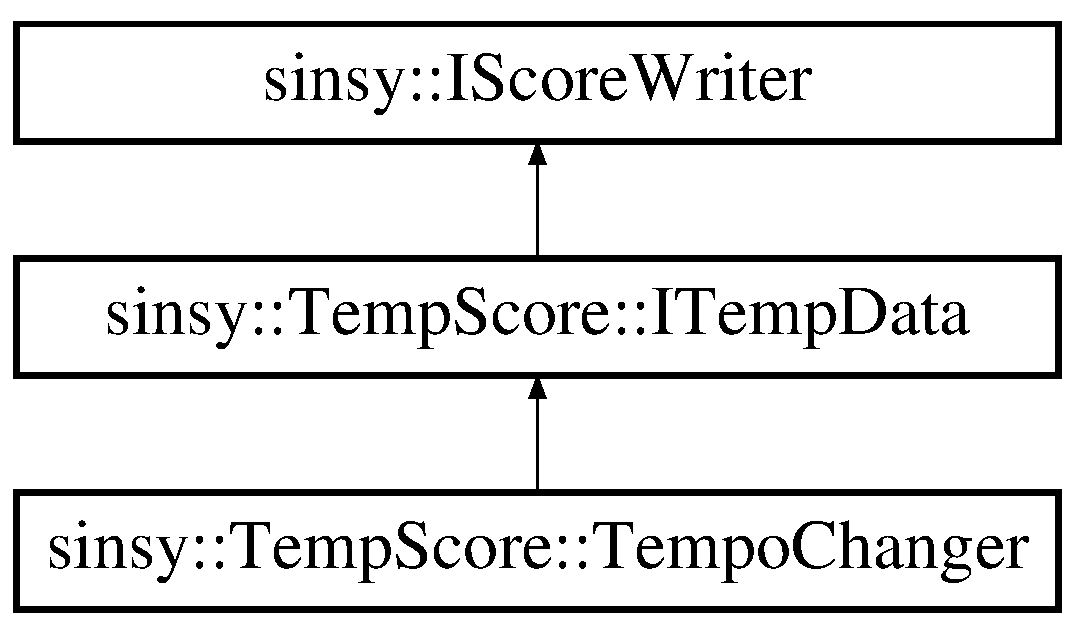
\includegraphics[height=3.000000cm]{classsinsy_1_1TempScore_1_1TempoChanger}
\end{center}
\end{figure}
\subsection*{\-Public \-Member \-Functions}
\begin{DoxyCompactItemize}
\item 
\hypertarget{classsinsy_1_1TempScore_1_1TempoChanger_aca8c98879a7c5efab64f25cd36438ad8}{\hyperlink{classsinsy_1_1TempScore_1_1TempoChanger_aca8c98879a7c5efab64f25cd36438ad8}{\-Tempo\-Changer} (double t)}\label{classsinsy_1_1TempScore_1_1TempoChanger_aca8c98879a7c5efab64f25cd36438ad8}

\begin{DoxyCompactList}\small\item\em constructor \end{DoxyCompactList}\item 
\hypertarget{classsinsy_1_1TempScore_1_1TempoChanger_abd747c15eb0a900af583ac87cd895e4b}{virtual \hyperlink{classsinsy_1_1TempScore_1_1TempoChanger_abd747c15eb0a900af583ac87cd895e4b}{$\sim$\-Tempo\-Changer} ()}\label{classsinsy_1_1TempScore_1_1TempoChanger_abd747c15eb0a900af583ac87cd895e4b}

\begin{DoxyCompactList}\small\item\em destructor \end{DoxyCompactList}\item 
\hypertarget{classsinsy_1_1TempScore_1_1TempoChanger_abf1ab4899af9c7a8780a39ca0d68909e}{virtual void \hyperlink{classsinsy_1_1TempScore_1_1TempoChanger_abf1ab4899af9c7a8780a39ca0d68909e}{write} (\hyperlink{classsinsy_1_1IScoreWritable}{\-I\-Score\-Writable} \&sm) const }\label{classsinsy_1_1TempScore_1_1TempoChanger_abf1ab4899af9c7a8780a39ca0d68909e}

\begin{DoxyCompactList}\small\item\em write \end{DoxyCompactList}\end{DoxyCompactItemize}


\-The documentation for this class was generated from the following files\-:\begin{DoxyCompactItemize}
\item 
lib/temporary/\-Temp\-Score.\-h\item 
lib/temporary/\-Temp\-Score.\-cpp\end{DoxyCompactItemize}

\hypertarget{classsinsy_1_1TempScore}{\section{sinsy\-:\-:\-Temp\-Score \-Class \-Reference}
\label{classsinsy_1_1TempScore}\index{sinsy\-::\-Temp\-Score@{sinsy\-::\-Temp\-Score}}
}
\-Inheritance diagram for sinsy\-:\-:\-Temp\-Score\-:\begin{figure}[H]
\begin{center}
\leavevmode
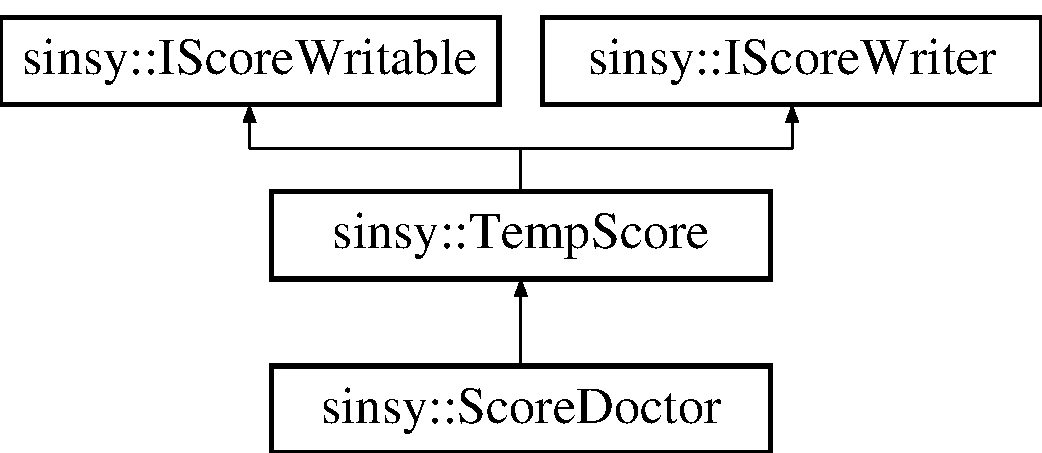
\includegraphics[height=3.000000cm]{classsinsy_1_1TempScore}
\end{center}
\end{figure}
\subsection*{\-Classes}
\begin{DoxyCompactItemize}
\item 
class \hyperlink{classsinsy_1_1TempScore_1_1BeatChanger}{\-Beat\-Changer}
\item 
class \hyperlink{classsinsy_1_1TempScore_1_1CrescendoStarter}{\-Crescendo\-Starter}
\item 
class \hyperlink{classsinsy_1_1TempScore_1_1CrescendoStopper}{\-Crescendo\-Stopper}
\item 
class {\bfseries \-Data\-Setter}
\item 
class \hyperlink{classsinsy_1_1TempScore_1_1DiminuendoStarter}{\-Diminuendo\-Starter}
\item 
class \hyperlink{classsinsy_1_1TempScore_1_1DiminuendoStopper}{\-Diminuendo\-Stopper}
\item 
class \hyperlink{classsinsy_1_1TempScore_1_1DynamicsChanger}{\-Dynamics\-Changer}
\item 
class \hyperlink{classsinsy_1_1TempScore_1_1EncodingSetter}{\-Encoding\-Setter}
\item 
class \hyperlink{classsinsy_1_1TempScore_1_1ITempData}{\-I\-Temp\-Data}
\item 
class \hyperlink{classsinsy_1_1TempScore_1_1KeyChanger}{\-Key\-Changer}
\item 
class \hyperlink{classsinsy_1_1TempScore_1_1NoteAdder}{\-Note\-Adder}
\item 
class \hyperlink{classsinsy_1_1TempScore_1_1TempoChanger}{\-Tempo\-Changer}
\end{DoxyCompactItemize}
\subsection*{\-Public \-Member \-Functions}
\begin{DoxyCompactItemize}
\item 
\hypertarget{classsinsy_1_1TempScore_a47727b37c6f229cf01ef456e0ac2337a}{\hyperlink{classsinsy_1_1TempScore_a47727b37c6f229cf01ef456e0ac2337a}{\-Temp\-Score} ()}\label{classsinsy_1_1TempScore_a47727b37c6f229cf01ef456e0ac2337a}

\begin{DoxyCompactList}\small\item\em constructor \end{DoxyCompactList}\item 
\hypertarget{classsinsy_1_1TempScore_a24397560d04ca9a85a7a62cc2b6376b9}{virtual \hyperlink{classsinsy_1_1TempScore_a24397560d04ca9a85a7a62cc2b6376b9}{$\sim$\-Temp\-Score} ()}\label{classsinsy_1_1TempScore_a24397560d04ca9a85a7a62cc2b6376b9}

\begin{DoxyCompactList}\small\item\em destructor \end{DoxyCompactList}\item 
\hypertarget{classsinsy_1_1TempScore_a47010b736dc38d71b14f6086588b15a0}{virtual void \hyperlink{classsinsy_1_1TempScore_a47010b736dc38d71b14f6086588b15a0}{clear} ()}\label{classsinsy_1_1TempScore_a47010b736dc38d71b14f6086588b15a0}

\begin{DoxyCompactList}\small\item\em clear \end{DoxyCompactList}\item 
\hypertarget{classsinsy_1_1TempScore_a51c129629b33b95bd37be34da9b0a080}{virtual void \hyperlink{classsinsy_1_1TempScore_a51c129629b33b95bd37be34da9b0a080}{write} (\hyperlink{classsinsy_1_1IScoreWritable}{\-I\-Score\-Writable} \&) const }\label{classsinsy_1_1TempScore_a51c129629b33b95bd37be34da9b0a080}

\begin{DoxyCompactList}\small\item\em write \end{DoxyCompactList}\item 
\hypertarget{classsinsy_1_1TempScore_a02321c0dcc624481b9c06d856c5e21eb}{virtual void \hyperlink{classsinsy_1_1TempScore_a02321c0dcc624481b9c06d856c5e21eb}{set\-Encoding} (const std\-::string \&e)}\label{classsinsy_1_1TempScore_a02321c0dcc624481b9c06d856c5e21eb}

\begin{DoxyCompactList}\small\item\em set encoding \end{DoxyCompactList}\item 
\hypertarget{classsinsy_1_1TempScore_ad8c1d34cebc7947b2e9e86fd02cff869}{virtual void \hyperlink{classsinsy_1_1TempScore_ad8c1d34cebc7947b2e9e86fd02cff869}{change\-Tempo} (double)}\label{classsinsy_1_1TempScore_ad8c1d34cebc7947b2e9e86fd02cff869}

\begin{DoxyCompactList}\small\item\em change tempo \end{DoxyCompactList}\item 
\hypertarget{classsinsy_1_1TempScore_aa9e3da3090018ac147517054acef3427}{virtual void \hyperlink{classsinsy_1_1TempScore_aa9e3da3090018ac147517054acef3427}{change\-Beat} (const \hyperlink{classsinsy_1_1Beat}{\-Beat} \&)}\label{classsinsy_1_1TempScore_aa9e3da3090018ac147517054acef3427}

\begin{DoxyCompactList}\small\item\em change beat \end{DoxyCompactList}\item 
\hypertarget{classsinsy_1_1TempScore_afe153ff53689214ab666d1988424bcd0}{virtual void \hyperlink{classsinsy_1_1TempScore_afe153ff53689214ab666d1988424bcd0}{change\-Dynamics} (const \hyperlink{classsinsy_1_1Dynamics}{\-Dynamics} \&)}\label{classsinsy_1_1TempScore_afe153ff53689214ab666d1988424bcd0}

\begin{DoxyCompactList}\small\item\em change dynamics \end{DoxyCompactList}\item 
\hypertarget{classsinsy_1_1TempScore_a003cbb4a65789b8448e683d13cdce460}{virtual void \hyperlink{classsinsy_1_1TempScore_a003cbb4a65789b8448e683d13cdce460}{change\-Key} (const \hyperlink{classsinsy_1_1Key}{\-Key} \&)}\label{classsinsy_1_1TempScore_a003cbb4a65789b8448e683d13cdce460}

\begin{DoxyCompactList}\small\item\em change key \end{DoxyCompactList}\item 
\hypertarget{classsinsy_1_1TempScore_a07c0e12e49f53cf22c0e113e0ba64c3d}{virtual void \hyperlink{classsinsy_1_1TempScore_a07c0e12e49f53cf22c0e113e0ba64c3d}{start\-Crescendo} ()}\label{classsinsy_1_1TempScore_a07c0e12e49f53cf22c0e113e0ba64c3d}

\begin{DoxyCompactList}\small\item\em start crescendo \end{DoxyCompactList}\item 
\hypertarget{classsinsy_1_1TempScore_addae25576d24053a0270f2ed98242d61}{virtual void \hyperlink{classsinsy_1_1TempScore_addae25576d24053a0270f2ed98242d61}{start\-Diminuendo} ()}\label{classsinsy_1_1TempScore_addae25576d24053a0270f2ed98242d61}

\begin{DoxyCompactList}\small\item\em start diminuendo \end{DoxyCompactList}\item 
\hypertarget{classsinsy_1_1TempScore_a4abb9125e2f1815aa13c5ca418f9cc9b}{virtual void \hyperlink{classsinsy_1_1TempScore_a4abb9125e2f1815aa13c5ca418f9cc9b}{stop\-Crescendo} ()}\label{classsinsy_1_1TempScore_a4abb9125e2f1815aa13c5ca418f9cc9b}

\begin{DoxyCompactList}\small\item\em stop crescendo \end{DoxyCompactList}\item 
\hypertarget{classsinsy_1_1TempScore_a7cf004fbf86eb6612aa560e7f0304d7b}{virtual void \hyperlink{classsinsy_1_1TempScore_a7cf004fbf86eb6612aa560e7f0304d7b}{stop\-Diminuendo} ()}\label{classsinsy_1_1TempScore_a7cf004fbf86eb6612aa560e7f0304d7b}

\begin{DoxyCompactList}\small\item\em stop diminuendo \end{DoxyCompactList}\item 
\hypertarget{classsinsy_1_1TempScore_a6976fe57e1a9a0b4c6861841a3f130bd}{virtual void \hyperlink{classsinsy_1_1TempScore_a6976fe57e1a9a0b4c6861841a3f130bd}{add\-Note} (const \hyperlink{classsinsy_1_1Note}{\-Note} \&)}\label{classsinsy_1_1TempScore_a6976fe57e1a9a0b4c6861841a3f130bd}

\begin{DoxyCompactList}\small\item\em add note \end{DoxyCompactList}\end{DoxyCompactItemize}
\subsection*{\-Protected \-Types}
\begin{DoxyCompactItemize}
\item 
\hypertarget{classsinsy_1_1TempScore_abf2f3b265a49049bd2728a6b0e7ea8cd}{typedef std\-::vector$<$ \hyperlink{classsinsy_1_1TempScore_1_1ITempData}{\-I\-Temp\-Data} $\ast$ $>$ {\bfseries \-Temp\-List}}\label{classsinsy_1_1TempScore_abf2f3b265a49049bd2728a6b0e7ea8cd}

\end{DoxyCompactItemize}
\subsection*{\-Protected \-Attributes}
\begin{DoxyCompactItemize}
\item 
\hypertarget{classsinsy_1_1TempScore_a990ea698c07d1a233466dc380c4e37d7}{\-Temp\-List \hyperlink{classsinsy_1_1TempScore_a990ea698c07d1a233466dc380c4e37d7}{temp\-List}}\label{classsinsy_1_1TempScore_a990ea698c07d1a233466dc380c4e37d7}

\begin{DoxyCompactList}\small\item\em list of temporaries \end{DoxyCompactList}\end{DoxyCompactItemize}


\-The documentation for this class was generated from the following files\-:\begin{DoxyCompactItemize}
\item 
lib/temporary/\-Temp\-Score.\-h\item 
lib/temporary/\-Temp\-Score.\-cpp\end{DoxyCompactItemize}

\hypertarget{classsinsy_1_1UnknownConf}{\section{sinsy\-:\-:\-Unknown\-Conf \-Class \-Reference}
\label{classsinsy_1_1UnknownConf}\index{sinsy\-::\-Unknown\-Conf@{sinsy\-::\-Unknown\-Conf}}
}
\-Inheritance diagram for sinsy\-:\-:\-Unknown\-Conf\-:\begin{figure}[H]
\begin{center}
\leavevmode
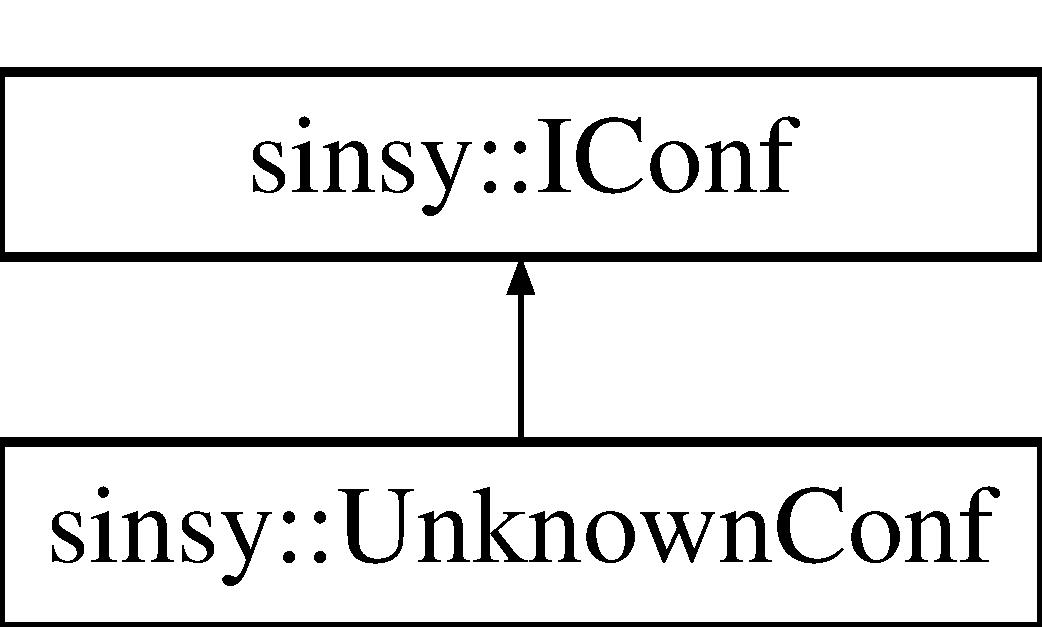
\includegraphics[height=2.000000cm]{classsinsy_1_1UnknownConf}
\end{center}
\end{figure}
\subsection*{\-Public \-Member \-Functions}
\begin{DoxyCompactItemize}
\item 
\hypertarget{classsinsy_1_1UnknownConf_a600c23683bb17dcc8c9f3481c7a097e4}{\hyperlink{classsinsy_1_1UnknownConf_a600c23683bb17dcc8c9f3481c7a097e4}{\-Unknown\-Conf} ()}\label{classsinsy_1_1UnknownConf_a600c23683bb17dcc8c9f3481c7a097e4}

\begin{DoxyCompactList}\small\item\em constructor \end{DoxyCompactList}\item 
\hypertarget{classsinsy_1_1UnknownConf_aa2f609daa15caa8cc9b76a04f90f9b84}{virtual \hyperlink{classsinsy_1_1UnknownConf_aa2f609daa15caa8cc9b76a04f90f9b84}{$\sim$\-Unknown\-Conf} ()}\label{classsinsy_1_1UnknownConf_aa2f609daa15caa8cc9b76a04f90f9b84}

\begin{DoxyCompactList}\small\item\em destructor \end{DoxyCompactList}\item 
virtual bool \hyperlink{classsinsy_1_1UnknownConf_aa3716c61e71716facd6b4ee74ad65f35}{convert} (const std\-::string \&enc, \-Convertable\-List\-::iterator begin, \-Convertable\-List\-::iterator end) const 
\begin{DoxyCompactList}\small\item\em convert lyrics to phonemes \end{DoxyCompactList}\item 
void \hyperlink{classsinsy_1_1UnknownConf_a192c80d61f64237d6efde75fa2979298}{clear} ()
\item 
virtual std\-::string \hyperlink{classsinsy_1_1UnknownConf_a011e2150d42ec96f593a3ee730430c2e}{get\-Sil\-Str} () const 
\begin{DoxyCompactList}\small\item\em get sil str \end{DoxyCompactList}\end{DoxyCompactItemize}


\subsection{\-Member \-Function \-Documentation}
\hypertarget{classsinsy_1_1UnknownConf_a192c80d61f64237d6efde75fa2979298}{\index{sinsy\-::\-Unknown\-Conf@{sinsy\-::\-Unknown\-Conf}!clear@{clear}}
\index{clear@{clear}!sinsy::UnknownConf@{sinsy\-::\-Unknown\-Conf}}
\subsubsection[{clear}]{\setlength{\rightskip}{0pt plus 5cm}void {\bf \-Unknown\-Conf\-::clear} (
\begin{DoxyParamCaption}
{}
\end{DoxyParamCaption}
)}}\label{classsinsy_1_1UnknownConf_a192c80d61f64237d6efde75fa2979298}
clear \hypertarget{classsinsy_1_1UnknownConf_aa3716c61e71716facd6b4ee74ad65f35}{\index{sinsy\-::\-Unknown\-Conf@{sinsy\-::\-Unknown\-Conf}!convert@{convert}}
\index{convert@{convert}!sinsy::UnknownConf@{sinsy\-::\-Unknown\-Conf}}
\subsubsection[{convert}]{\setlength{\rightskip}{0pt plus 5cm}bool {\bf \-Unknown\-Conf\-::convert} (
\begin{DoxyParamCaption}
\item[{const std\-::string \&}]{enc, }
\item[{\-Convertable\-List\-::iterator}]{begin, }
\item[{\-Convertable\-List\-::iterator}]{end}
\end{DoxyParamCaption}
) const\hspace{0.3cm}{\ttfamily  \mbox{[}virtual\mbox{]}}}}\label{classsinsy_1_1UnknownConf_aa3716c61e71716facd6b4ee74ad65f35}


convert lyrics to phonemes 

convert lyrics to phonemes


\begin{DoxyParams}{\-Parameters}
{\em enc} & encoding \\
\hline
{\em begin} & start of note list \\
\hline
{\em end} & last of note list \\
\hline
\end{DoxyParams}
\begin{DoxyReturn}{\-Returns}
if success, return true 
\end{DoxyReturn}


\-Implements \hyperlink{classsinsy_1_1IConf_a892ad5cc8098a0b2bb720deade6dc0ee}{sinsy\-::\-I\-Conf}.

\hypertarget{classsinsy_1_1UnknownConf_a011e2150d42ec96f593a3ee730430c2e}{\index{sinsy\-::\-Unknown\-Conf@{sinsy\-::\-Unknown\-Conf}!get\-Sil\-Str@{get\-Sil\-Str}}
\index{get\-Sil\-Str@{get\-Sil\-Str}!sinsy::UnknownConf@{sinsy\-::\-Unknown\-Conf}}
\subsubsection[{get\-Sil\-Str}]{\setlength{\rightskip}{0pt plus 5cm}std\-::string {\bf \-Unknown\-Conf\-::get\-Sil\-Str} (
\begin{DoxyParamCaption}
{}
\end{DoxyParamCaption}
) const\hspace{0.3cm}{\ttfamily  \mbox{[}virtual\mbox{]}}}}\label{classsinsy_1_1UnknownConf_a011e2150d42ec96f593a3ee730430c2e}


get sil str 

get sil str

return edge rest 

\-Implements \hyperlink{classsinsy_1_1IConf_a6b4b753e87291960ccc88867d97ef280}{sinsy\-::\-I\-Conf}.



\-The documentation for this class was generated from the following files\-:\begin{DoxyCompactItemize}
\item 
lib/converter/\-Unknown\-Conf.\-h\item 
lib/converter/\-Unknown\-Conf.\-cpp\end{DoxyCompactItemize}

\hypertarget{classsinsy_1_1WritableStrStream}{\section{sinsy\-:\-:\-Writable\-Str\-Stream \-Class \-Reference}
\label{classsinsy_1_1WritableStrStream}\index{sinsy\-::\-Writable\-Str\-Stream@{sinsy\-::\-Writable\-Str\-Stream}}
}
\subsection*{\-Public \-Member \-Functions}
\begin{DoxyCompactItemize}
\item 
\hypertarget{classsinsy_1_1WritableStrStream_a669548a8de107bab0a0c13972569757a}{\hyperlink{classsinsy_1_1WritableStrStream_a669548a8de107bab0a0c13972569757a}{\-Writable\-Str\-Stream} (\hyperlink{classsinsy_1_1IWritableStream}{\-I\-Writable\-Stream} \&s)}\label{classsinsy_1_1WritableStrStream_a669548a8de107bab0a0c13972569757a}

\begin{DoxyCompactList}\small\item\em constructor \end{DoxyCompactList}\item 
\hypertarget{classsinsy_1_1WritableStrStream_a758fd45156c859552c94497889209844}{virtual \hyperlink{classsinsy_1_1WritableStrStream_a758fd45156c859552c94497889209844}{$\sim$\-Writable\-Str\-Stream} ()}\label{classsinsy_1_1WritableStrStream_a758fd45156c859552c94497889209844}

\begin{DoxyCompactList}\small\item\em destructor \end{DoxyCompactList}\item 
{\footnotesize template$<$class T $>$ }\\\hyperlink{classsinsy_1_1WritableStrStream}{\-Writable\-Str\-Stream} \& \hyperlink{classsinsy_1_1WritableStrStream_a64c44dccf4d749780734e35582a75a84}{operator$<$$<$} (const \-T \&buf)  throw (\-Stream\-Exception)
\end{DoxyCompactItemize}


\subsection{\-Member \-Function \-Documentation}
\hypertarget{classsinsy_1_1WritableStrStream_a64c44dccf4d749780734e35582a75a84}{\index{sinsy\-::\-Writable\-Str\-Stream@{sinsy\-::\-Writable\-Str\-Stream}!operator$<$$<$@{operator$<$$<$}}
\index{operator$<$$<$@{operator$<$$<$}!sinsy::WritableStrStream@{sinsy\-::\-Writable\-Str\-Stream}}
\subsubsection[{operator$<$$<$}]{\setlength{\rightskip}{0pt plus 5cm}template$<$class T $>$ {\bf \-Writable\-Str\-Stream}\& sinsy\-::\-Writable\-Str\-Stream\-::operator$<$$<$ (
\begin{DoxyParamCaption}
\item[{const \-T \&}]{buf}
\end{DoxyParamCaption}
)  throw ({\bf \-Stream\-Exception})\hspace{0.3cm}{\ttfamily  \mbox{[}inline\mbox{]}}}}\label{classsinsy_1_1WritableStrStream_a64c44dccf4d749780734e35582a75a84}
convert data to string and write to stream 

\-The documentation for this class was generated from the following file\-:\begin{DoxyCompactItemize}
\item 
lib/util/\-Writable\-Str\-Stream.\-h\end{DoxyCompactItemize}

\hypertarget{classsinsy_1_1XmlData}{\section{sinsy\-:\-:\-Xml\-Data \-Class \-Reference}
\label{classsinsy_1_1XmlData}\index{sinsy\-::\-Xml\-Data@{sinsy\-::\-Xml\-Data}}
}
\-Inheritance diagram for sinsy\-:\-:\-Xml\-Data\-:\begin{figure}[H]
\begin{center}
\leavevmode
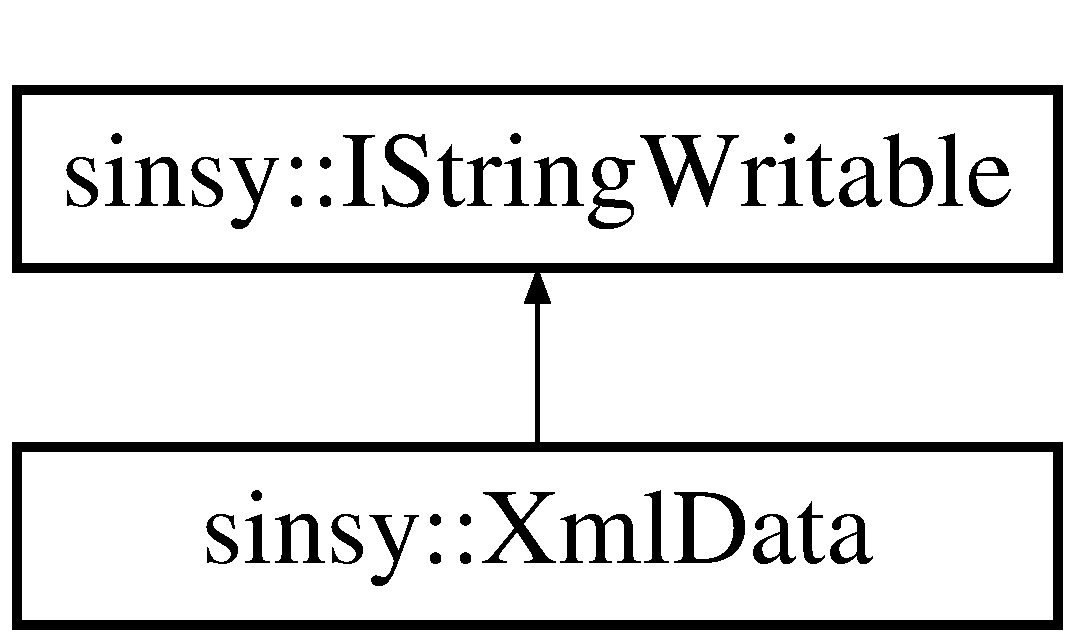
\includegraphics[height=2.000000cm]{classsinsy_1_1XmlData}
\end{center}
\end{figure}
\subsection*{\-Public \-Types}
\begin{DoxyCompactItemize}
\item 
\hypertarget{classsinsy_1_1XmlData_acd4c1a20bf66dfc7f8a6728e2df3400a}{typedef std\-::vector$<$ \hyperlink{classsinsy_1_1XmlData}{\-Xml\-Data} $\ast$ $>$ {\bfseries \-Children}}\label{classsinsy_1_1XmlData_acd4c1a20bf66dfc7f8a6728e2df3400a}

\end{DoxyCompactItemize}
\subsection*{\-Public \-Member \-Functions}
\begin{DoxyCompactItemize}
\item 
\hyperlink{classsinsy_1_1XmlData_abe69d904133fe8a99ae013a41418ab72}{\-Xml\-Data} (const std\-::string \&t, const std\-::string \&d=\char`\"{}\char`\"{})
\begin{DoxyCompactList}\small\item\em constructor \end{DoxyCompactList}\item 
\hypertarget{classsinsy_1_1XmlData_a4548ecce1cc5b2b26fcb30aba716d42a}{\hyperlink{classsinsy_1_1XmlData_a4548ecce1cc5b2b26fcb30aba716d42a}{\-Xml\-Data} (const \hyperlink{classsinsy_1_1XmlData}{\-Xml\-Data} \&)}\label{classsinsy_1_1XmlData_a4548ecce1cc5b2b26fcb30aba716d42a}

\begin{DoxyCompactList}\small\item\em copy constructor \end{DoxyCompactList}\item 
\hypertarget{classsinsy_1_1XmlData_a847aa0938ae7466fbcface61c883ecd8}{virtual \hyperlink{classsinsy_1_1XmlData_a847aa0938ae7466fbcface61c883ecd8}{$\sim$\-Xml\-Data} ()}\label{classsinsy_1_1XmlData_a847aa0938ae7466fbcface61c883ecd8}

\begin{DoxyCompactList}\small\item\em destructor \end{DoxyCompactList}\item 
\hypertarget{classsinsy_1_1XmlData_aa9dcc99c122404a684e6c333f9e6070a}{const std\-::string \& \hyperlink{classsinsy_1_1XmlData_aa9dcc99c122404a684e6c333f9e6070a}{get\-Tag} () const }\label{classsinsy_1_1XmlData_aa9dcc99c122404a684e6c333f9e6070a}

\begin{DoxyCompactList}\small\item\em get tag \end{DoxyCompactList}\item 
\hypertarget{classsinsy_1_1XmlData_ae3f90a3ad85b374848e1fe0fb427101f}{const std\-::string \& \hyperlink{classsinsy_1_1XmlData_ae3f90a3ad85b374848e1fe0fb427101f}{get\-Data} () const }\label{classsinsy_1_1XmlData_ae3f90a3ad85b374848e1fe0fb427101f}

\begin{DoxyCompactList}\small\item\em get data \end{DoxyCompactList}\item 
\hypertarget{classsinsy_1_1XmlData_a41e71f4fc6991539947a6aed54eec70a}{void \hyperlink{classsinsy_1_1XmlData_a41e71f4fc6991539947a6aed54eec70a}{set\-Data} (const std\-::string \&str)}\label{classsinsy_1_1XmlData_a41e71f4fc6991539947a6aed54eec70a}

\begin{DoxyCompactList}\small\item\em set data \end{DoxyCompactList}\item 
\hypertarget{classsinsy_1_1XmlData_a41c44b99462fb6cdc8dfae815c2c0ea2}{void \hyperlink{classsinsy_1_1XmlData_a41c44b99462fb6cdc8dfae815c2c0ea2}{add\-Child} (\hyperlink{classsinsy_1_1XmlData}{\-Xml\-Data} $\ast$child)}\label{classsinsy_1_1XmlData_a41c44b99462fb6cdc8dfae815c2c0ea2}

\begin{DoxyCompactList}\small\item\em add child \end{DoxyCompactList}\item 
\hypertarget{classsinsy_1_1XmlData_a857e8a855483e2465d46d86d7d360ef0}{\-Xml\-Data\-::\-Children\-::iterator \hyperlink{classsinsy_1_1XmlData_a857e8a855483e2465d46d86d7d360ef0}{erase\-Child} (const \-Children\-::iterator \&itr)}\label{classsinsy_1_1XmlData_a857e8a855483e2465d46d86d7d360ef0}

\begin{DoxyCompactList}\small\item\em erase child \end{DoxyCompactList}\item 
\hypertarget{classsinsy_1_1XmlData_ab42614836cefbe72aa7d5b69fa4e1412}{bool \hyperlink{classsinsy_1_1XmlData_ab42614836cefbe72aa7d5b69fa4e1412}{add\-Attribute} (const std\-::string \&k, const std\-::string \&v)}\label{classsinsy_1_1XmlData_ab42614836cefbe72aa7d5b69fa4e1412}

\begin{DoxyCompactList}\small\item\em add attribute \end{DoxyCompactList}\item 
\hypertarget{classsinsy_1_1XmlData_af935830732afe0dbb556673cc392c35b}{const std\-::string \& \hyperlink{classsinsy_1_1XmlData_af935830732afe0dbb556673cc392c35b}{get\-Attribute} (const std\-::string \&k) const }\label{classsinsy_1_1XmlData_af935830732afe0dbb556673cc392c35b}

\begin{DoxyCompactList}\small\item\em get attribute \end{DoxyCompactList}\item 
std\-::ostream \& \hyperlink{classsinsy_1_1XmlData_a7b725f824cf3b8dc6509f09303cdb07d}{to\-String\-Stream} (std\-::ostream \&os) const 
\begin{DoxyCompactList}\small\item\em push into stringstream \end{DoxyCompactList}\item 
\hypertarget{classsinsy_1_1XmlData_aabe43178ad0c9e454f51902bcc48b652}{\-Children\-::const\-\_\-iterator \hyperlink{classsinsy_1_1XmlData_aabe43178ad0c9e454f51902bcc48b652}{child\-Begin} () const }\label{classsinsy_1_1XmlData_aabe43178ad0c9e454f51902bcc48b652}

\begin{DoxyCompactList}\small\item\em get begin const iterator of children \end{DoxyCompactList}\item 
\hypertarget{classsinsy_1_1XmlData_ab79636503b6def5fa0c82687fccfd125}{\-Children\-::const\-\_\-iterator \hyperlink{classsinsy_1_1XmlData_ab79636503b6def5fa0c82687fccfd125}{child\-End} () const }\label{classsinsy_1_1XmlData_ab79636503b6def5fa0c82687fccfd125}

\begin{DoxyCompactList}\small\item\em get end const iterator of children \end{DoxyCompactList}\item 
\hypertarget{classsinsy_1_1XmlData_a6cb8ea8defe501fcd5ff8b5f0cacbd4b}{\-Children\-::iterator \hyperlink{classsinsy_1_1XmlData_a6cb8ea8defe501fcd5ff8b5f0cacbd4b}{child\-Begin} ()}\label{classsinsy_1_1XmlData_a6cb8ea8defe501fcd5ff8b5f0cacbd4b}

\begin{DoxyCompactList}\small\item\em get begin iterator of children \end{DoxyCompactList}\item 
\hypertarget{classsinsy_1_1XmlData_a0585083e072004b3008bf2f01f5b47b3}{\-Children\-::iterator \hyperlink{classsinsy_1_1XmlData_a0585083e072004b3008bf2f01f5b47b3}{child\-End} ()}\label{classsinsy_1_1XmlData_a0585083e072004b3008bf2f01f5b47b3}

\begin{DoxyCompactList}\small\item\em get end iterator of children \end{DoxyCompactList}\end{DoxyCompactItemize}


\subsection{\-Constructor \& \-Destructor \-Documentation}
\hypertarget{classsinsy_1_1XmlData_abe69d904133fe8a99ae013a41418ab72}{\index{sinsy\-::\-Xml\-Data@{sinsy\-::\-Xml\-Data}!\-Xml\-Data@{\-Xml\-Data}}
\index{\-Xml\-Data@{\-Xml\-Data}!sinsy::XmlData@{sinsy\-::\-Xml\-Data}}
\subsubsection[{\-Xml\-Data}]{\setlength{\rightskip}{0pt plus 5cm}{\bf \-Xml\-Data\-::\-Xml\-Data} (
\begin{DoxyParamCaption}
\item[{const std\-::string \&}]{t, }
\item[{const std\-::string \&}]{d = {\ttfamily \char`\"{}\char`\"{}}}
\end{DoxyParamCaption}
)}}\label{classsinsy_1_1XmlData_abe69d904133fe8a99ae013a41418ab72}


constructor 

constructor


\begin{DoxyParams}{\-Parameters}
{\em t} & tag \\
\hline
{\em d} & data \\
\hline
\end{DoxyParams}


\subsection{\-Member \-Function \-Documentation}
\hypertarget{classsinsy_1_1XmlData_a7b725f824cf3b8dc6509f09303cdb07d}{\index{sinsy\-::\-Xml\-Data@{sinsy\-::\-Xml\-Data}!to\-String\-Stream@{to\-String\-Stream}}
\index{to\-String\-Stream@{to\-String\-Stream}!sinsy::XmlData@{sinsy\-::\-Xml\-Data}}
\subsubsection[{to\-String\-Stream}]{\setlength{\rightskip}{0pt plus 5cm}std\-::ostream \& {\bf \-Xml\-Data\-::to\-String\-Stream} (
\begin{DoxyParamCaption}
\item[{std\-::ostream \&}]{stream}
\end{DoxyParamCaption}
) const\hspace{0.3cm}{\ttfamily  \mbox{[}virtual\mbox{]}}}}\label{classsinsy_1_1XmlData_a7b725f824cf3b8dc6509f09303cdb07d}


push into stringstream 

to string stream 

\-Implements \hyperlink{classsinsy_1_1IStringWritable_a044c5bb33002dacec9bbdbf2dc0fbe23}{sinsy\-::\-I\-String\-Writable}.



\-The documentation for this class was generated from the following files\-:\begin{DoxyCompactItemize}
\item 
lib/xml/\-Xml\-Data.\-h\item 
lib/xml/\-Xml\-Data.\-cpp\end{DoxyCompactItemize}

\hypertarget{classsinsy_1_1XmlParser}{\section{sinsy\-:\-:\-Xml\-Parser \-Class \-Reference}
\label{classsinsy_1_1XmlParser}\index{sinsy\-::\-Xml\-Parser@{sinsy\-::\-Xml\-Parser}}
}
\subsection*{\-Public \-Member \-Functions}
\begin{DoxyCompactItemize}
\item 
\hypertarget{classsinsy_1_1XmlParser_ac77b14a84c93a07288b7dcd9d3a17397}{\hyperlink{classsinsy_1_1XmlParser_ac77b14a84c93a07288b7dcd9d3a17397}{\-Xml\-Parser} ()}\label{classsinsy_1_1XmlParser_ac77b14a84c93a07288b7dcd9d3a17397}

\begin{DoxyCompactList}\small\item\em constructor \end{DoxyCompactList}\item 
\hypertarget{classsinsy_1_1XmlParser_ae3078c5ea3b5c79258a92513b55d8511}{virtual \hyperlink{classsinsy_1_1XmlParser_ae3078c5ea3b5c79258a92513b55d8511}{$\sim$\-Xml\-Parser} ()}\label{classsinsy_1_1XmlParser_ae3078c5ea3b5c79258a92513b55d8511}

\begin{DoxyCompactList}\small\item\em destructor \end{DoxyCompactList}\item 
\hyperlink{classsinsy_1_1XmlData}{\-Xml\-Data} $\ast$ \hyperlink{classsinsy_1_1XmlParser_ab286d37a8c7e35b0b0621c4b7320db42}{read} (\hyperlink{classsinsy_1_1IReadableStream}{\-I\-Readable\-Stream} \&stream, std\-::string \&encoding)  throw (\-Stream\-Exception)
\begin{DoxyCompactList}\small\item\em read xml from stream \end{DoxyCompactList}\end{DoxyCompactItemize}


\subsection{\-Member \-Function \-Documentation}
\hypertarget{classsinsy_1_1XmlParser_ab286d37a8c7e35b0b0621c4b7320db42}{\index{sinsy\-::\-Xml\-Parser@{sinsy\-::\-Xml\-Parser}!read@{read}}
\index{read@{read}!sinsy::XmlParser@{sinsy\-::\-Xml\-Parser}}
\subsubsection[{read}]{\setlength{\rightskip}{0pt plus 5cm}{\bf \-Xml\-Data} $\ast$ {\bf \-Xml\-Parser\-::read} (
\begin{DoxyParamCaption}
\item[{{\bf \-I\-Readable\-Stream} \&}]{stream, }
\item[{std\-::string \&}]{encoding}
\end{DoxyParamCaption}
)  throw ({\bf \-Stream\-Exception})}}\label{classsinsy_1_1XmlParser_ab286d37a8c7e35b0b0621c4b7320db42}


read xml from stream 

read data from stream 

\-The documentation for this class was generated from the following files\-:\begin{DoxyCompactItemize}
\item 
lib/xml/\-Xml\-Parser.\-h\item 
lib/xml/\-Xml\-Parser.\-cpp\end{DoxyCompactItemize}

\hypertarget{classsinsy_1_1XmlReader}{\section{sinsy\-:\-:\-Xml\-Reader \-Class \-Reference}
\label{classsinsy_1_1XmlReader}\index{sinsy\-::\-Xml\-Reader@{sinsy\-::\-Xml\-Reader}}
}
\-Inheritance diagram for sinsy\-:\-:\-Xml\-Reader\-:\begin{figure}[H]
\begin{center}
\leavevmode
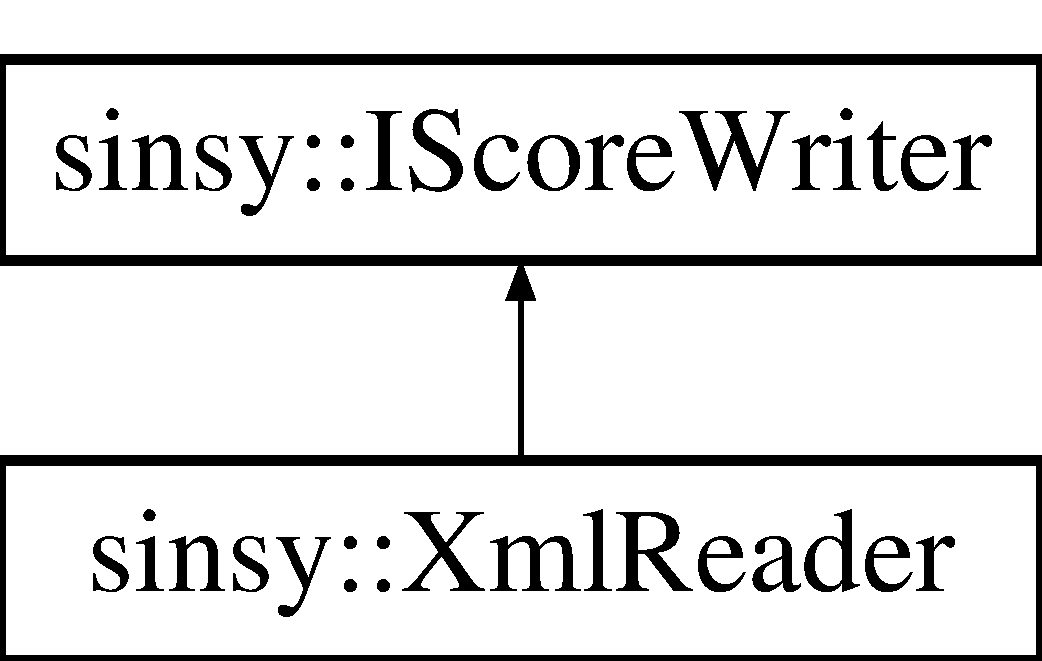
\includegraphics[height=2.000000cm]{classsinsy_1_1XmlReader}
\end{center}
\end{figure}
\subsection*{\-Public \-Member \-Functions}
\begin{DoxyCompactItemize}
\item 
\hypertarget{classsinsy_1_1XmlReader_adac676393e3a2500ccd901b6c4283962}{\hyperlink{classsinsy_1_1XmlReader_adac676393e3a2500ccd901b6c4283962}{\-Xml\-Reader} ()}\label{classsinsy_1_1XmlReader_adac676393e3a2500ccd901b6c4283962}

\begin{DoxyCompactList}\small\item\em constructor \end{DoxyCompactList}\item 
\hypertarget{classsinsy_1_1XmlReader_a8903e46b5682f43a291617886a9b1fbf}{virtual \hyperlink{classsinsy_1_1XmlReader_a8903e46b5682f43a291617886a9b1fbf}{$\sim$\-Xml\-Reader} ()}\label{classsinsy_1_1XmlReader_a8903e46b5682f43a291617886a9b1fbf}

\begin{DoxyCompactList}\small\item\em destructor \end{DoxyCompactList}\item 
void \hyperlink{classsinsy_1_1XmlReader_a6758ead0eea59bf9babf340f2a2aea83}{clear} ()
\begin{DoxyCompactList}\small\item\em clear; \end{DoxyCompactList}\item 
void \hyperlink{classsinsy_1_1XmlReader_acf02eb4794dfbad6e1b71d5cd7221a52}{write} (\hyperlink{classsinsy_1_1IScoreWritable}{\-I\-Score\-Writable} \&writable) const 
\begin{DoxyCompactList}\small\item\em write to score (operator $<$$<$ should be used) \end{DoxyCompactList}\item 
bool \hyperlink{classsinsy_1_1XmlReader_a0b08ba6f27e900555de9173872882fa2}{read\-Xml} (\hyperlink{classsinsy_1_1IReadableStream}{\-I\-Readable\-Stream} \&stream)
\begin{DoxyCompactList}\small\item\em read xml from stream \end{DoxyCompactList}\item 
\hypertarget{classsinsy_1_1XmlReader_adcda3d45e5ac86d336b3b2cf44cfc60e}{const \hyperlink{classsinsy_1_1XmlData}{\-Xml\-Data} $\ast$ \hyperlink{classsinsy_1_1XmlReader_adcda3d45e5ac86d336b3b2cf44cfc60e}{get\-Xml\-Data} () const }\label{classsinsy_1_1XmlReader_adcda3d45e5ac86d336b3b2cf44cfc60e}

\begin{DoxyCompactList}\small\item\em get xml data \end{DoxyCompactList}\end{DoxyCompactItemize}


\subsection{\-Member \-Function \-Documentation}
\hypertarget{classsinsy_1_1XmlReader_a6758ead0eea59bf9babf340f2a2aea83}{\index{sinsy\-::\-Xml\-Reader@{sinsy\-::\-Xml\-Reader}!clear@{clear}}
\index{clear@{clear}!sinsy::XmlReader@{sinsy\-::\-Xml\-Reader}}
\subsubsection[{clear}]{\setlength{\rightskip}{0pt plus 5cm}void {\bf \-Xml\-Reader\-::clear} (
\begin{DoxyParamCaption}
{}
\end{DoxyParamCaption}
)}}\label{classsinsy_1_1XmlReader_a6758ead0eea59bf9babf340f2a2aea83}


clear; 

clear \hypertarget{classsinsy_1_1XmlReader_a0b08ba6f27e900555de9173872882fa2}{\index{sinsy\-::\-Xml\-Reader@{sinsy\-::\-Xml\-Reader}!read\-Xml@{read\-Xml}}
\index{read\-Xml@{read\-Xml}!sinsy::XmlReader@{sinsy\-::\-Xml\-Reader}}
\subsubsection[{read\-Xml}]{\setlength{\rightskip}{0pt plus 5cm}bool {\bf \-Xml\-Reader\-::read\-Xml} (
\begin{DoxyParamCaption}
\item[{{\bf \-I\-Readable\-Stream} \&}]{stream}
\end{DoxyParamCaption}
)}}\label{classsinsy_1_1XmlReader_a0b08ba6f27e900555de9173872882fa2}


read xml from stream 

read xml from stream


\begin{DoxyParams}{\-Parameters}
{\em stream} & input stream \\
\hline
\end{DoxyParams}
\begin{DoxyReturn}{\-Returns}
if success, true 
\end{DoxyReturn}
\hypertarget{classsinsy_1_1XmlReader_acf02eb4794dfbad6e1b71d5cd7221a52}{\index{sinsy\-::\-Xml\-Reader@{sinsy\-::\-Xml\-Reader}!write@{write}}
\index{write@{write}!sinsy::XmlReader@{sinsy\-::\-Xml\-Reader}}
\subsubsection[{write}]{\setlength{\rightskip}{0pt plus 5cm}void {\bf \-Xml\-Reader\-::write} (
\begin{DoxyParamCaption}
\item[{{\bf \-I\-Score\-Writable} \&}]{writable}
\end{DoxyParamCaption}
) const\hspace{0.3cm}{\ttfamily  \mbox{[}virtual\mbox{]}}}}\label{classsinsy_1_1XmlReader_acf02eb4794dfbad6e1b71d5cd7221a52}


write to score (operator $<$$<$ should be used) 

write score 

\-Implements \hyperlink{classsinsy_1_1IScoreWriter_a15b81f3e78834610052da3cc48e0f7ad}{sinsy\-::\-I\-Score\-Writer}.



\-The documentation for this class was generated from the following files\-:\begin{DoxyCompactItemize}
\item 
lib/xml/\-Xml\-Reader.\-h\item 
lib/xml/\-Xml\-Reader.\-cpp\end{DoxyCompactItemize}

\hypertarget{classsinsy_1_1XmlWriter}{\section{sinsy\-:\-:\-Xml\-Writer \-Class \-Reference}
\label{classsinsy_1_1XmlWriter}\index{sinsy\-::\-Xml\-Writer@{sinsy\-::\-Xml\-Writer}}
}
\-Inheritance diagram for sinsy\-:\-:\-Xml\-Writer\-:\begin{figure}[H]
\begin{center}
\leavevmode
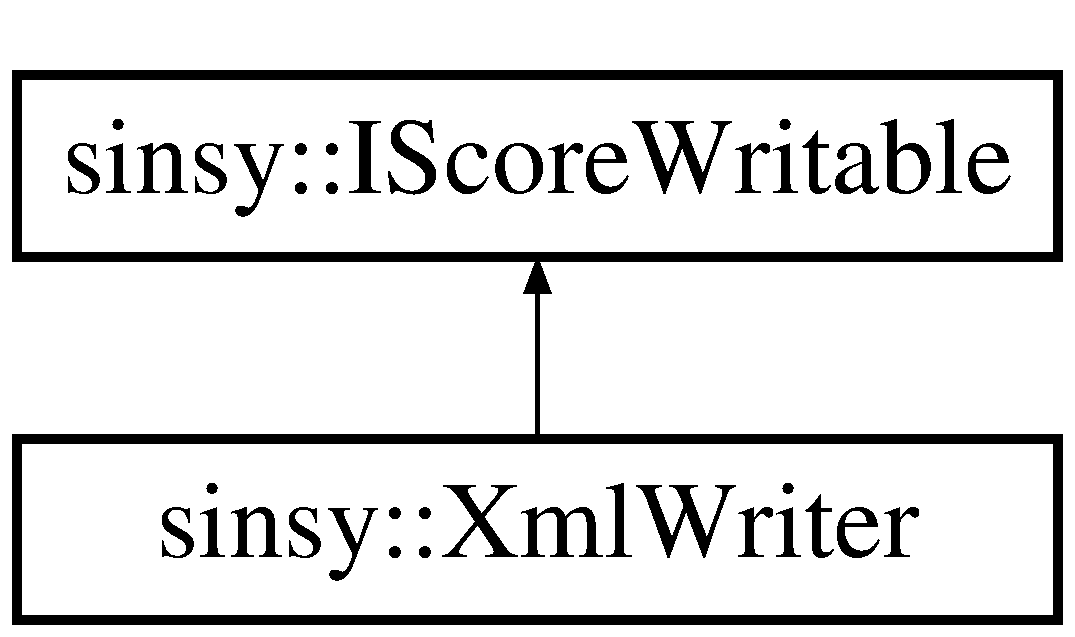
\includegraphics[height=2.000000cm]{classsinsy_1_1XmlWriter}
\end{center}
\end{figure}
\subsection*{\-Public \-Member \-Functions}
\begin{DoxyCompactItemize}
\item 
\hypertarget{classsinsy_1_1XmlWriter_ae3462f88219ba977efe6bf4f671d6083}{\hyperlink{classsinsy_1_1XmlWriter_ae3462f88219ba977efe6bf4f671d6083}{\-Xml\-Writer} ()}\label{classsinsy_1_1XmlWriter_ae3462f88219ba977efe6bf4f671d6083}

\begin{DoxyCompactList}\small\item\em constructor \end{DoxyCompactList}\item 
\hypertarget{classsinsy_1_1XmlWriter_a5fad7b65b620dad44be1d3521cd4d4f9}{virtual \hyperlink{classsinsy_1_1XmlWriter_a5fad7b65b620dad44be1d3521cd4d4f9}{$\sim$\-Xml\-Writer} ()}\label{classsinsy_1_1XmlWriter_a5fad7b65b620dad44be1d3521cd4d4f9}

\begin{DoxyCompactList}\small\item\em destructor \end{DoxyCompactList}\item 
void \hyperlink{classsinsy_1_1XmlWriter_a20aeea8e8105ef55855816fe4ee87b03}{clear} ()
\begin{DoxyCompactList}\small\item\em clear; \end{DoxyCompactList}\item 
\hypertarget{classsinsy_1_1XmlWriter_a8d05b1d4963923228db8283cc1e0c9df}{const \hyperlink{classsinsy_1_1XmlData}{\-Xml\-Data} $\ast$ \hyperlink{classsinsy_1_1XmlWriter_a8d05b1d4963923228db8283cc1e0c9df}{get\-Xml\-Data} () const }\label{classsinsy_1_1XmlWriter_a8d05b1d4963923228db8283cc1e0c9df}

\begin{DoxyCompactList}\small\item\em get xml data \end{DoxyCompactList}\item 
virtual void \hyperlink{classsinsy_1_1XmlWriter_a65bf2c52e895553fa4f23f641c5c71e8}{set\-Encoding} (const std\-::string \&encoding)
\item 
\hypertarget{classsinsy_1_1XmlWriter_ab87f15d2f3345bc2edeae4db85651234}{virtual void \hyperlink{classsinsy_1_1XmlWriter_ab87f15d2f3345bc2edeae4db85651234}{change\-Tempo} (double tempo)}\label{classsinsy_1_1XmlWriter_ab87f15d2f3345bc2edeae4db85651234}

\begin{DoxyCompactList}\small\item\em change tempo \end{DoxyCompactList}\item 
\hypertarget{classsinsy_1_1XmlWriter_aa7cda2d4ca24d8c44f7857ad07fdc12d}{virtual void \hyperlink{classsinsy_1_1XmlWriter_aa7cda2d4ca24d8c44f7857ad07fdc12d}{change\-Beat} (const \hyperlink{classsinsy_1_1Beat}{\-Beat} \&beat)}\label{classsinsy_1_1XmlWriter_aa7cda2d4ca24d8c44f7857ad07fdc12d}

\begin{DoxyCompactList}\small\item\em change beat \end{DoxyCompactList}\item 
\hypertarget{classsinsy_1_1XmlWriter_a9ed65ff1f8586a11e1e524f62c2feda0}{virtual void \hyperlink{classsinsy_1_1XmlWriter_a9ed65ff1f8586a11e1e524f62c2feda0}{change\-Dynamics} (const \hyperlink{classsinsy_1_1Dynamics}{\-Dynamics} \&dynamics)}\label{classsinsy_1_1XmlWriter_a9ed65ff1f8586a11e1e524f62c2feda0}

\begin{DoxyCompactList}\small\item\em change dynamics \end{DoxyCompactList}\item 
\hypertarget{classsinsy_1_1XmlWriter_ad5ced923386aa1be0a82745a1e337c14}{virtual void \hyperlink{classsinsy_1_1XmlWriter_ad5ced923386aa1be0a82745a1e337c14}{change\-Key} (const \hyperlink{classsinsy_1_1Key}{\-Key} \&key)}\label{classsinsy_1_1XmlWriter_ad5ced923386aa1be0a82745a1e337c14}

\begin{DoxyCompactList}\small\item\em change key \end{DoxyCompactList}\item 
\hypertarget{classsinsy_1_1XmlWriter_a7e8343646c0744f95da6afc0cd1208e5}{virtual void \hyperlink{classsinsy_1_1XmlWriter_a7e8343646c0744f95da6afc0cd1208e5}{start\-Crescendo} ()}\label{classsinsy_1_1XmlWriter_a7e8343646c0744f95da6afc0cd1208e5}

\begin{DoxyCompactList}\small\item\em start crescendo \end{DoxyCompactList}\item 
\hypertarget{classsinsy_1_1XmlWriter_af542af35a9d957caa4886ab182d9ac55}{virtual void \hyperlink{classsinsy_1_1XmlWriter_af542af35a9d957caa4886ab182d9ac55}{start\-Diminuendo} ()}\label{classsinsy_1_1XmlWriter_af542af35a9d957caa4886ab182d9ac55}

\begin{DoxyCompactList}\small\item\em start diminuendo \end{DoxyCompactList}\item 
\hypertarget{classsinsy_1_1XmlWriter_a37018ef9f5d8bb816c0b3281033a9262}{virtual void \hyperlink{classsinsy_1_1XmlWriter_a37018ef9f5d8bb816c0b3281033a9262}{stop\-Crescendo} ()}\label{classsinsy_1_1XmlWriter_a37018ef9f5d8bb816c0b3281033a9262}

\begin{DoxyCompactList}\small\item\em stop crescendo \end{DoxyCompactList}\item 
\hypertarget{classsinsy_1_1XmlWriter_a9c5ebcc1a7936584655980894e21b330}{virtual void \hyperlink{classsinsy_1_1XmlWriter_a9c5ebcc1a7936584655980894e21b330}{stop\-Diminuendo} ()}\label{classsinsy_1_1XmlWriter_a9c5ebcc1a7936584655980894e21b330}

\begin{DoxyCompactList}\small\item\em stop diminuendo \end{DoxyCompactList}\item 
\hypertarget{classsinsy_1_1XmlWriter_a73938135557c30d8a0ce7f6e42388fb8}{virtual void \hyperlink{classsinsy_1_1XmlWriter_a73938135557c30d8a0ce7f6e42388fb8}{add\-Note} (const \hyperlink{classsinsy_1_1Note}{\-Note} \&note)}\label{classsinsy_1_1XmlWriter_a73938135557c30d8a0ce7f6e42388fb8}

\begin{DoxyCompactList}\small\item\em add note \end{DoxyCompactList}\item 
bool \hyperlink{classsinsy_1_1XmlWriter_aad09698ce393de49f083666ee26cfd0a}{write\-Xml} (\hyperlink{classsinsy_1_1WritableStrStream}{\-Writable\-Str\-Stream} \&stream) const 
\begin{DoxyCompactList}\small\item\em write xml to stream \end{DoxyCompactList}\item 
bool \hyperlink{classsinsy_1_1XmlWriter_aebe855c816e53dd765f461213d802608}{write\-Xml} (\hyperlink{classsinsy_1_1WritableStrStream}{\-Writable\-Str\-Stream} \&stream, const \hyperlink{classsinsy_1_1XmlData}{\-Xml\-Data} \&orig\-Data\-\_\-)
\begin{DoxyCompactList}\small\item\em write xml to stream using original xml \end{DoxyCompactList}\end{DoxyCompactItemize}


\subsection{\-Member \-Function \-Documentation}
\hypertarget{classsinsy_1_1XmlWriter_a20aeea8e8105ef55855816fe4ee87b03}{\index{sinsy\-::\-Xml\-Writer@{sinsy\-::\-Xml\-Writer}!clear@{clear}}
\index{clear@{clear}!sinsy::XmlWriter@{sinsy\-::\-Xml\-Writer}}
\subsubsection[{clear}]{\setlength{\rightskip}{0pt plus 5cm}void {\bf \-Xml\-Writer\-::clear} (
\begin{DoxyParamCaption}
{}
\end{DoxyParamCaption}
)}}\label{classsinsy_1_1XmlWriter_a20aeea8e8105ef55855816fe4ee87b03}


clear; 

clear \hypertarget{classsinsy_1_1XmlWriter_a65bf2c52e895553fa4f23f641c5c71e8}{\index{sinsy\-::\-Xml\-Writer@{sinsy\-::\-Xml\-Writer}!set\-Encoding@{set\-Encoding}}
\index{set\-Encoding@{set\-Encoding}!sinsy::XmlWriter@{sinsy\-::\-Xml\-Writer}}
\subsubsection[{set\-Encoding}]{\setlength{\rightskip}{0pt plus 5cm}void {\bf \-Xml\-Writer\-::set\-Encoding} (
\begin{DoxyParamCaption}
\item[{const std\-::string \&}]{enc}
\end{DoxyParamCaption}
)\hspace{0.3cm}{\ttfamily  \mbox{[}virtual\mbox{]}}}}\label{classsinsy_1_1XmlWriter_a65bf2c52e895553fa4f23f641c5c71e8}
set encoding 

\-Implements \hyperlink{classsinsy_1_1IScoreWritable}{sinsy\-::\-I\-Score\-Writable}.

\hypertarget{classsinsy_1_1XmlWriter_aad09698ce393de49f083666ee26cfd0a}{\index{sinsy\-::\-Xml\-Writer@{sinsy\-::\-Xml\-Writer}!write\-Xml@{write\-Xml}}
\index{write\-Xml@{write\-Xml}!sinsy::XmlWriter@{sinsy\-::\-Xml\-Writer}}
\subsubsection[{write\-Xml}]{\setlength{\rightskip}{0pt plus 5cm}bool {\bf \-Xml\-Writer\-::write\-Xml} (
\begin{DoxyParamCaption}
\item[{{\bf \-Writable\-Str\-Stream} \&}]{stream}
\end{DoxyParamCaption}
) const}}\label{classsinsy_1_1XmlWriter_aad09698ce393de49f083666ee26cfd0a}


write xml to stream 

write xml to stream


\begin{DoxyParams}{\-Parameters}
{\em stream} & output stream \\
\hline
\end{DoxyParams}
\begin{DoxyReturn}{\-Returns}
if success, true 
\end{DoxyReturn}
\hypertarget{classsinsy_1_1XmlWriter_aebe855c816e53dd765f461213d802608}{\index{sinsy\-::\-Xml\-Writer@{sinsy\-::\-Xml\-Writer}!write\-Xml@{write\-Xml}}
\index{write\-Xml@{write\-Xml}!sinsy::XmlWriter@{sinsy\-::\-Xml\-Writer}}
\subsubsection[{write\-Xml}]{\setlength{\rightskip}{0pt plus 5cm}bool {\bf \-Xml\-Writer\-::write\-Xml} (
\begin{DoxyParamCaption}
\item[{{\bf \-Writable\-Str\-Stream} \&}]{stream, }
\item[{const {\bf \-Xml\-Data} \&}]{orig\-Data\-\_\-}
\end{DoxyParamCaption}
)}}\label{classsinsy_1_1XmlWriter_aebe855c816e53dd765f461213d802608}


write xml to stream using original xml 

write xml to stream using original xml


\begin{DoxyParams}{\-Parameters}
{\em stream} & output stream  oroginal \-Music\-X\-M\-L \\
\hline
\end{DoxyParams}
\begin{DoxyReturn}{\-Returns}
if success, true 
\end{DoxyReturn}


\-The documentation for this class was generated from the following files\-:\begin{DoxyCompactItemize}
\item 
lib/xml/\-Xml\-Writer.\-h\item 
lib/xml/\-Xml\-Writer.\-cpp\end{DoxyCompactItemize}

\printindex
\end{document}
